\documentclass[twoside]{book}

% Packages required by doxygen
\usepackage{fixltx2e}
\usepackage{calc}
\usepackage{doxygen}
\usepackage[export]{adjustbox} % also loads graphicx
\usepackage{graphicx}
\usepackage[utf8]{inputenc}
\usepackage{makeidx}
\usepackage{multicol}
\usepackage{multirow}
\PassOptionsToPackage{warn}{textcomp}
\usepackage{textcomp}
\usepackage[nointegrals]{wasysym}
\usepackage[table]{xcolor}

% Font selection
\usepackage[T1]{fontenc}
\usepackage[scaled=.90]{helvet}
\usepackage{courier}
\usepackage{amssymb}
\usepackage{sectsty}
\renewcommand{\familydefault}{\sfdefault}
\allsectionsfont{%
  \fontseries{bc}\selectfont%
  \color{darkgray}%
}
\renewcommand{\DoxyLabelFont}{%
  \fontseries{bc}\selectfont%
  \color{darkgray}%
}
\newcommand{\+}{\discretionary{\mbox{\scriptsize$\hookleftarrow$}}{}{}}

% Page & text layout
\usepackage{geometry}
\geometry{%
  a4paper,%
  top=2.5cm,%
  bottom=2.5cm,%
  left=2.5cm,%
  right=2.5cm%
}
\tolerance=750
\hfuzz=15pt
\hbadness=750
\setlength{\emergencystretch}{15pt}
\setlength{\parindent}{0cm}
\setlength{\parskip}{3ex plus 2ex minus 2ex}
\makeatletter
\renewcommand{\paragraph}{%
  \@startsection{paragraph}{4}{0ex}{-1.0ex}{1.0ex}{%
    \normalfont\normalsize\bfseries\SS@parafont%
  }%
}
\renewcommand{\subparagraph}{%
  \@startsection{subparagraph}{5}{0ex}{-1.0ex}{1.0ex}{%
    \normalfont\normalsize\bfseries\SS@subparafont%
  }%
}
\makeatother

% Headers & footers
\usepackage{fancyhdr}
\pagestyle{fancyplain}
\fancyhead[LE]{\fancyplain{}{\bfseries\thepage}}
\fancyhead[CE]{\fancyplain{}{}}
\fancyhead[RE]{\fancyplain{}{\bfseries\leftmark}}
\fancyhead[LO]{\fancyplain{}{\bfseries\rightmark}}
\fancyhead[CO]{\fancyplain{}{}}
\fancyhead[RO]{\fancyplain{}{\bfseries\thepage}}
\fancyfoot[LE]{\fancyplain{}{}}
\fancyfoot[CE]{\fancyplain{}{}}
\fancyfoot[RE]{\fancyplain{}{\bfseries\scriptsize Generated by Doxygen }}
\fancyfoot[LO]{\fancyplain{}{\bfseries\scriptsize Generated by Doxygen }}
\fancyfoot[CO]{\fancyplain{}{}}
\fancyfoot[RO]{\fancyplain{}{}}
\renewcommand{\footrulewidth}{0.4pt}
\renewcommand{\chaptermark}[1]{%
  \markboth{#1}{}%
}
\renewcommand{\sectionmark}[1]{%
  \markright{\thesection\ #1}%
}

% Indices & bibliography
\usepackage{natbib}
\usepackage[titles]{tocloft}
\setcounter{tocdepth}{3}
\setcounter{secnumdepth}{5}
\makeindex

% Hyperlinks (required, but should be loaded last)
\usepackage{ifpdf}
\ifpdf
  \usepackage[pdftex,pagebackref=true]{hyperref}
\else
  \usepackage[ps2pdf,pagebackref=true]{hyperref}
\fi
\hypersetup{%
  colorlinks=true,%
  linkcolor=blue,%
  citecolor=blue,%
  unicode%
}

% Custom commands
\newcommand{\clearemptydoublepage}{%
  \newpage{\pagestyle{empty}\cleardoublepage}%
}

\usepackage{caption}
\captionsetup{labelsep=space,justification=centering,font={bf},singlelinecheck=off,skip=4pt,position=top}

%===== C O N T E N T S =====

\begin{document}

% Titlepage & ToC
\hypersetup{pageanchor=false,
             bookmarksnumbered=true,
             pdfencoding=unicode
            }
\pagenumbering{alph}
\begin{titlepage}
\vspace*{7cm}
\begin{center}%
{\Large lxm32 }\\
\vspace*{1cm}
{\large Generated by Doxygen 1.8.13}\\
\end{center}
\end{titlepage}
\clearemptydoublepage
\pagenumbering{roman}
\tableofcontents
\clearemptydoublepage
\pagenumbering{arabic}
\hypersetup{pageanchor=true}

%--- Begin generated contents ---
\chapter{canopen}
\label{md__home_adev__documents__s_t_e_c_h_lxm32_lib_canopen__r_e_a_d_m_e}
\Hypertarget{md__home_adev__documents__s_t_e_c_h_lxm32_lib_canopen__r_e_a_d_m_e}
\subsection*{Information}


\begin{DoxyItemize}
\item {\bfseries Brief}\+: Canopen object able to send command through a C\+AN interface using the U\+N\+IX socket.
\item {\bfseries Languages}\+: C++
\item {\bfseries Libraries}\+:
\item {\bfseries Note}\+: /
\item {\bfseries Compatibility}\+:
\end{DoxyItemize}

\tabulinesep=1mm
\begin{longtabu} spread 0pt [c]{*{3}{|X[-1]}|}
\hline
\rowcolor{\tableheadbgcolor}\PBS\centering \textbf{ Ubuntu }&\PBS\centering \textbf{ Window10 }&\PBS\centering \textbf{ Mac\+OS  }\\\cline{1-3}
\endfirsthead
\hline
\endfoot
\hline
\rowcolor{\tableheadbgcolor}\PBS\centering \textbf{ Ubuntu }&\PBS\centering \textbf{ Window10 }&\PBS\centering \textbf{ Mac\+OS  }\\\cline{1-3}
\endhead
\PBS\centering \+:heavy\+\_\+check\+\_\+mark\+:&\PBS\centering \+:grey\+\_\+question\+:&\PBS\centering \+:grey\+\_\+question\+: \\\cline{1-3}
\end{longtabu}


\subsection*{Building}

\subsubsection*{Ubuntu}

\paragraph*{Steps}


\begin{DoxyItemize}
\item Clone the repository and go inside. 
\begin{DoxyCode}
git clone https://gitlab-dev.isir.upmc.fr/devillard/canopen.git && cd canpen
\end{DoxyCode}

\item Create a build directory and go inside.
\item Configure the project.
\item Build the project. 
\begin{DoxyCode}
mkdir build && cd build && cmake .. && cmake --build .
\end{DoxyCode}

\end{DoxyItemize}

\paragraph*{Testing}

\#\#\#\#\# Install can tools 
\begin{DoxyCode}
sudo apt install can-utilis
\end{DoxyCode}


\#\#\#\#\# Setup a virtual C\+AN bus 
\begin{DoxyCode}
sudo ip link add dev vcan0 type vcan && ip link set up vcan0
\end{DoxyCode}


\#\#\#\#\# Listen to the C\+AN bus 
\begin{DoxyCode}
candump vcan0
\end{DoxyCode}


\subsection*{Canopen program}

The executable file canopen enable you to send S\+DO message to a C\+AN bus. \subsubsection*{usage\+:}

./canopen ifname 0xindex 0xsub \mbox{[} size base data \mbox{]}

Arg\+: ifname \+: C\+AN interface name 0xindex \+: Object register index 0xsub \+: Object register subindex size \+: Data size (number of bytes) base \+: Numerical base of the value passed. data \+: Value to write.

Ex\+: To read register 0x1000\+:2 of node 4 on \char`\"{}can0\char`\"{}\+: ./canopen can0 4 1000 2

To write in register 0x2000\+:F of node 3 the value 0x1234 on \char`\"{}can0\char`\"{}\+: ./canopen can0 3 2000 F 2 x 1234 
\chapter{joystick}
\label{md__home_adev__documents__s_t_e_c_h_lxm32_lib_joystick__r_e_a_d_m_e}
\Hypertarget{md__home_adev__documents__s_t_e_c_h_lxm32_lib_joystick__r_e_a_d_m_e}
\input{md__home_adev__documents__s_t_e_c_h_lxm32_lib_joystick__r_e_a_d_m_e}
\chapter{lxm32}
\label{md__home_adev__documents__s_t_e_c_h_lxm32__r_e_a_d_m_e}
\Hypertarget{md__home_adev__documents__s_t_e_c_h_lxm32__r_e_a_d_m_e}
\subsection*{Information}


\begin{DoxyItemize}
\item {\bfseries Brief}\+: Library to control a Lexium32A driver from Schneider.
\item {\bfseries Languages}\+: C++
\item {\bfseries Libraries}\+:
\item {\bfseries Note}\+: /
\item {\bfseries Compatibility}\+:
\end{DoxyItemize}

\tabulinesep=1mm
\begin{longtabu} spread 0pt [c]{*{3}{|X[-1]}|}
\hline
\rowcolor{\tableheadbgcolor}\PBS\centering \textbf{ Ubuntu }&\PBS\centering \textbf{ Window10 }&\PBS\centering \textbf{ Mac\+OS  }\\\cline{1-3}
\endfirsthead
\hline
\endfoot
\hline
\rowcolor{\tableheadbgcolor}\PBS\centering \textbf{ Ubuntu }&\PBS\centering \textbf{ Window10 }&\PBS\centering \textbf{ Mac\+OS  }\\\cline{1-3}
\endhead
\PBS\centering \+:heavy\+\_\+check\+\_\+mark\+:&\PBS\centering \+:grey\+\_\+question\+:&\PBS\centering \+:grey\+\_\+question\+: \\\cline{1-3}
\end{longtabu}


\subsection*{Building}

\subsubsection*{Ubuntu}

\paragraph*{Steps}


\begin{DoxyItemize}
\item Clone the repository and go inside. 
\begin{DoxyCode}
git clone https://gitlab-dev.isir.upmc.fr/devillard/lxm32.git && cd lxm32
\end{DoxyCode}

\item Create a build directory and go inside.
\item Configure the project.
\item Build the project. 
\begin{DoxyCode}
mkdir build && cd build && cmake .. && cmake --build .
\end{DoxyCode}

\end{DoxyItemize}

\subsection*{Schematics}

  
\chapter{Namespace Index}
\section{Namespace List}
Here is a list of all namespaces with brief descriptions\+:\begin{DoxyCompactList}
\item\contentsline{section}{\hyperlink{namespace_c_a_nopen}{C\+A\+Nopen} }{\pageref{namespace_c_a_nopen}}{}
\end{DoxyCompactList}

\chapter{Hierarchical Index}
\section{Class Hierarchy}
This inheritance list is sorted roughly, but not completely, alphabetically\+:\begin{DoxyCompactList}
\item can\+\_\+frame\begin{DoxyCompactList}
\item \contentsline{section}{C\+A\+Nopen\+:\+:Message}{\pageref{class_c_a_nopen_1_1_message}}{}
\begin{DoxyCompactList}
\item \contentsline{section}{C\+A\+Nopen\+:\+:N\+M\+T\+Message}{\pageref{class_c_a_nopen_1_1_n_m_t_message}}{}
\item \contentsline{section}{C\+A\+Nopen\+:\+:P\+D\+O\+Message}{\pageref{class_c_a_nopen_1_1_p_d_o_message}}{}
\item \contentsline{section}{C\+A\+Nopen\+:\+:S\+D\+O\+Message}{\pageref{class_c_a_nopen_1_1_s_d_o_message}}{}
\begin{DoxyCompactList}
\item \contentsline{section}{C\+A\+Nopen\+:\+:S\+D\+O\+Inbound}{\pageref{class_c_a_nopen_1_1_s_d_o_inbound}}{}
\item \contentsline{section}{C\+A\+Nopen\+:\+:S\+D\+O\+Outbound}{\pageref{class_c_a_nopen_1_1_s_d_o_outbound}}{}
\begin{DoxyCompactList}
\item \contentsline{section}{C\+A\+Nopen\+:\+:S\+D\+O\+Outbound\+Read}{\pageref{class_c_a_nopen_1_1_s_d_o_outbound_read}}{}
\item \contentsline{section}{C\+A\+Nopen\+:\+:S\+D\+O\+Outbound\+Write}{\pageref{class_c_a_nopen_1_1_s_d_o_outbound_write}}{}
\end{DoxyCompactList}
\end{DoxyCompactList}
\end{DoxyCompactList}
\end{DoxyCompactList}
\item \contentsline{section}{c\+Joystick}{\pageref{classc_joystick}}{}
\item \contentsline{section}{C\+A\+Nopen\+:\+:Driver}{\pageref{class_c_a_nopen_1_1_driver}}{}
\begin{DoxyCompactList}
\item \contentsline{section}{C\+A\+Nopen\+:\+:L\+X\+M32}{\pageref{class_c_a_nopen_1_1_l_x_m32}}{}
\end{DoxyCompactList}
\item \contentsline{section}{joystick\+\_\+position}{\pageref{structjoystick__position}}{}
\item \contentsline{section}{joystick\+\_\+state}{\pageref{structjoystick__state}}{}
\item \contentsline{section}{C\+A\+Nopen\+:\+:Socket}{\pageref{class_c_a_nopen_1_1_socket}}{}
\item \contentsline{section}{sss$<$ T $>$}{\pageref{structsss}}{}
\item vector\begin{DoxyCompactList}
\item \contentsline{section}{C\+A\+Nopen\+:\+:Payload}{\pageref{class_c_a_nopen_1_1_payload}}{}
\end{DoxyCompactList}
\end{DoxyCompactList}

\chapter{Class Index}
\section{Class List}
Here are the classes, structs, unions and interfaces with brief descriptions\+:\begin{DoxyCompactList}
\item\contentsline{section}{\hyperlink{classc_joystick}{c\+Joystick} }{\pageref{classc_joystick}}{}
\item\contentsline{section}{\hyperlink{class_c_a_nopen_1_1_driver}{C\+A\+Nopen\+::\+Driver} }{\pageref{class_c_a_nopen_1_1_driver}}{}
\item\contentsline{section}{\hyperlink{structjoystick__position}{joystick\+\_\+position} }{\pageref{structjoystick__position}}{}
\item\contentsline{section}{\hyperlink{structjoystick__state}{joystick\+\_\+state} }{\pageref{structjoystick__state}}{}
\item\contentsline{section}{\hyperlink{class_c_a_nopen_1_1_l_x_m32}{C\+A\+Nopen\+::\+L\+X\+M32} }{\pageref{class_c_a_nopen_1_1_l_x_m32}}{}
\item\contentsline{section}{\hyperlink{class_c_a_nopen_1_1_message}{C\+A\+Nopen\+::\+Message} }{\pageref{class_c_a_nopen_1_1_message}}{}
\item\contentsline{section}{\hyperlink{class_c_a_nopen_1_1_n_m_t_message}{C\+A\+Nopen\+::\+N\+M\+T\+Message} }{\pageref{class_c_a_nopen_1_1_n_m_t_message}}{}
\item\contentsline{section}{\hyperlink{class_c_a_nopen_1_1_payload}{C\+A\+Nopen\+::\+Payload} }{\pageref{class_c_a_nopen_1_1_payload}}{}
\item\contentsline{section}{\hyperlink{class_c_a_nopen_1_1_p_d_o_message}{C\+A\+Nopen\+::\+P\+D\+O\+Message} }{\pageref{class_c_a_nopen_1_1_p_d_o_message}}{}
\item\contentsline{section}{\hyperlink{class_c_a_nopen_1_1_s_d_o_inbound}{C\+A\+Nopen\+::\+S\+D\+O\+Inbound} }{\pageref{class_c_a_nopen_1_1_s_d_o_inbound}}{}
\item\contentsline{section}{\hyperlink{class_c_a_nopen_1_1_s_d_o_message}{C\+A\+Nopen\+::\+S\+D\+O\+Message} }{\pageref{class_c_a_nopen_1_1_s_d_o_message}}{}
\item\contentsline{section}{\hyperlink{class_c_a_nopen_1_1_s_d_o_outbound}{C\+A\+Nopen\+::\+S\+D\+O\+Outbound} }{\pageref{class_c_a_nopen_1_1_s_d_o_outbound}}{}
\item\contentsline{section}{\hyperlink{class_c_a_nopen_1_1_s_d_o_outbound_read}{C\+A\+Nopen\+::\+S\+D\+O\+Outbound\+Read} }{\pageref{class_c_a_nopen_1_1_s_d_o_outbound_read}}{}
\item\contentsline{section}{\hyperlink{class_c_a_nopen_1_1_s_d_o_outbound_write}{C\+A\+Nopen\+::\+S\+D\+O\+Outbound\+Write} }{\pageref{class_c_a_nopen_1_1_s_d_o_outbound_write}}{}
\item\contentsline{section}{\hyperlink{class_c_a_nopen_1_1_socket}{C\+A\+Nopen\+::\+Socket} \\*Canopen object able to send command through a C\+AN interface using U\+N\+IX sockets }{\pageref{class_c_a_nopen_1_1_socket}}{}
\item\contentsline{section}{\hyperlink{structsss}{sss$<$ T $>$} }{\pageref{structsss}}{}
\end{DoxyCompactList}

\chapter{File Index}
\section{File List}
Here is a list of all files with brief descriptions\+:\begin{DoxyCompactList}
\item\contentsline{section}{/home/adev/\+Documents/\+S\+T\+E\+C\+H/lxm32/build/\+C\+Make\+Files/\hyperlink{feature__tests_8c}{feature\+\_\+tests.\+c} }{\pageref{feature__tests_8c}}{}
\item\contentsline{section}{/home/adev/\+Documents/\+S\+T\+E\+C\+H/lxm32/build/\+C\+Make\+Files/\hyperlink{feature__tests_8cxx}{feature\+\_\+tests.\+cxx} }{\pageref{feature__tests_8cxx}}{}
\item\contentsline{section}{/home/adev/\+Documents/\+S\+T\+E\+C\+H/lxm32/build/\+C\+Make\+Files/3.\+10.\+2/\+Compiler\+Id\+C/\hyperlink{_c_make_c_compiler_id_8c}{C\+Make\+C\+Compiler\+Id.\+c} }{\pageref{_c_make_c_compiler_id_8c}}{}
\item\contentsline{section}{/home/adev/\+Documents/\+S\+T\+E\+C\+H/lxm32/build/\+C\+Make\+Files/3.\+10.\+2/\+Compiler\+Id\+C\+X\+X/\hyperlink{_c_make_c_x_x_compiler_id_8cpp}{C\+Make\+C\+X\+X\+Compiler\+Id.\+cpp} }{\pageref{_c_make_c_x_x_compiler_id_8cpp}}{}
\item\contentsline{section}{/home/adev/\+Documents/\+S\+T\+E\+C\+H/lxm32/include/\hyperlink{_c_a_ndriver_8h}{C\+A\+Ndriver.\+h} }{\pageref{_c_a_ndriver_8h}}{}
\item\contentsline{section}{/home/adev/\+Documents/\+S\+T\+E\+C\+H/lxm32/include/\hyperlink{_c_a_nopen__driver_8h}{C\+A\+Nopen\+\_\+driver.\+h} }{\pageref{_c_a_nopen__driver_8h}}{}
\item\contentsline{section}{/home/adev/\+Documents/\+S\+T\+E\+C\+H/lxm32/include/\hyperlink{_c_a_nopen__lxm32_8h}{C\+A\+Nopen\+\_\+lxm32.\+h} }{\pageref{_c_a_nopen__lxm32_8h}}{}
\item\contentsline{section}{/home/adev/\+Documents/\+S\+T\+E\+C\+H/lxm32/lib/canopen/include/\hyperlink{_c_a_nopen__socket_8h}{C\+A\+Nopen\+\_\+socket.\+h} \\*Canopen object able to send command through a C\+AN interface using the U\+N\+IX socket }{\pageref{_c_a_nopen__socket_8h}}{}
\item\contentsline{section}{/home/adev/\+Documents/\+S\+T\+E\+C\+H/lxm32/lib/canopen/include/\hyperlink{config_8h}{config.\+h} }{\pageref{config_8h}}{}
\item\contentsline{section}{/home/adev/\+Documents/\+S\+T\+E\+C\+H/lxm32/lib/canopen/include/\hyperlink{message_8h}{message.\+h} }{\pageref{message_8h}}{}
\item\contentsline{section}{/home/adev/\+Documents/\+S\+T\+E\+C\+H/lxm32/lib/canopen/include/\hyperlink{nmt_8h}{nmt.\+h} }{\pageref{nmt_8h}}{}
\item\contentsline{section}{/home/adev/\+Documents/\+S\+T\+E\+C\+H/lxm32/lib/canopen/include/\hyperlink{payload_8h}{payload.\+h} }{\pageref{payload_8h}}{}
\item\contentsline{section}{/home/adev/\+Documents/\+S\+T\+E\+C\+H/lxm32/lib/canopen/include/\hyperlink{pdo_8h}{pdo.\+h} }{\pageref{pdo_8h}}{}
\item\contentsline{section}{/home/adev/\+Documents/\+S\+T\+E\+C\+H/lxm32/lib/canopen/include/\hyperlink{sdo_8h}{sdo.\+h} }{\pageref{sdo_8h}}{}
\item\contentsline{section}{/home/adev/\+Documents/\+S\+T\+E\+C\+H/lxm32/lib/canopen/src/\hyperlink{_c_a_nopen__socket_8cpp}{C\+A\+Nopen\+\_\+socket.\+cpp} }{\pageref{_c_a_nopen__socket_8cpp}}{}
\item\contentsline{section}{/home/adev/\+Documents/\+S\+T\+E\+C\+H/lxm32/lib/canopen/src/\hyperlink{lib_2canopen_2src_2main_8cpp}{main.\+cpp} }{\pageref{lib_2canopen_2src_2main_8cpp}}{}
\item\contentsline{section}{/home/adev/\+Documents/\+S\+T\+E\+C\+H/lxm32/lib/canopen/src/\hyperlink{message_8cpp}{message.\+cpp} }{\pageref{message_8cpp}}{}
\item\contentsline{section}{/home/adev/\+Documents/\+S\+T\+E\+C\+H/lxm32/lib/canopen/src/\hyperlink{nmt_8cpp}{nmt.\+cpp} }{\pageref{nmt_8cpp}}{}
\item\contentsline{section}{/home/adev/\+Documents/\+S\+T\+E\+C\+H/lxm32/lib/canopen/src/\hyperlink{payload_8cpp}{payload.\+cpp} }{\pageref{payload_8cpp}}{}
\item\contentsline{section}{/home/adev/\+Documents/\+S\+T\+E\+C\+H/lxm32/lib/canopen/src/\hyperlink{pdo_8cpp}{pdo.\+cpp} }{\pageref{pdo_8cpp}}{}
\item\contentsline{section}{/home/adev/\+Documents/\+S\+T\+E\+C\+H/lxm32/lib/canopen/src/\hyperlink{sdo_8cpp}{sdo.\+cpp} }{\pageref{sdo_8cpp}}{}
\item\contentsline{section}{/home/adev/\+Documents/\+S\+T\+E\+C\+H/lxm32/lib/joystick/include/\hyperlink{joystick_8h}{joystick.\+h} }{\pageref{joystick_8h}}{}
\item\contentsline{section}{/home/adev/\+Documents/\+S\+T\+E\+C\+H/lxm32/lib/joystick/src/\hyperlink{joystick_8cpp}{joystick.\+cpp} }{\pageref{joystick_8cpp}}{}
\item\contentsline{section}{/home/adev/\+Documents/\+S\+T\+E\+C\+H/lxm32/lib/joystick/src/\hyperlink{lib_2joystick_2src_2main_8cpp}{main.\+cpp} }{\pageref{lib_2joystick_2src_2main_8cpp}}{}
\item\contentsline{section}{/home/adev/\+Documents/\+S\+T\+E\+C\+H/lxm32/src/\hyperlink{_c_a_nopen__driver_8cpp}{C\+A\+Nopen\+\_\+driver.\+cpp} }{\pageref{_c_a_nopen__driver_8cpp}}{}
\item\contentsline{section}{/home/adev/\+Documents/\+S\+T\+E\+C\+H/lxm32/src/\hyperlink{_c_a_nopen__lxm32_8cpp}{C\+A\+Nopen\+\_\+lxm32.\+cpp} }{\pageref{_c_a_nopen__lxm32_8cpp}}{}
\item\contentsline{section}{/home/adev/\+Documents/\+S\+T\+E\+C\+H/lxm32/src/\hyperlink{src_2main_8cpp}{main.\+cpp} }{\pageref{src_2main_8cpp}}{}
\end{DoxyCompactList}

\chapter{Namespace Documentation}
\hypertarget{namespace_c_a_nopen}{}\section{C\+A\+Nopen Namespace Reference}
\label{namespace_c_a_nopen}\index{C\+A\+Nopen@{C\+A\+Nopen}}
\subsection*{Classes}
\begin{DoxyCompactItemize}
\item 
class \hyperlink{class_c_a_nopen_1_1_driver}{Driver}
\item 
class \hyperlink{class_c_a_nopen_1_1_l_x_m32}{L\+X\+M32}
\item 
class \hyperlink{class_c_a_nopen_1_1_message}{Message}
\item 
class \hyperlink{class_c_a_nopen_1_1_n_m_t_message}{N\+M\+T\+Message}
\item 
class \hyperlink{class_c_a_nopen_1_1_payload}{Payload}
\item 
class \hyperlink{class_c_a_nopen_1_1_p_d_o_message}{P\+D\+O\+Message}
\item 
class \hyperlink{class_c_a_nopen_1_1_s_d_o_inbound}{S\+D\+O\+Inbound}
\item 
class \hyperlink{class_c_a_nopen_1_1_s_d_o_message}{S\+D\+O\+Message}
\item 
class \hyperlink{class_c_a_nopen_1_1_s_d_o_outbound}{S\+D\+O\+Outbound}
\item 
class \hyperlink{class_c_a_nopen_1_1_s_d_o_outbound_read}{S\+D\+O\+Outbound\+Read}
\item 
class \hyperlink{class_c_a_nopen_1_1_s_d_o_outbound_write}{S\+D\+O\+Outbound\+Write}
\item 
class \hyperlink{class_c_a_nopen_1_1_socket}{Socket}
\begin{DoxyCompactList}\small\item\em Canopen object able to send command through a C\+AN interface using U\+N\+IX sockets. \end{DoxyCompactList}\end{DoxyCompactItemize}

\chapter{Class Documentation}
\hypertarget{classc_joystick}{}\section{c\+Joystick Class Reference}
\label{classc_joystick}\index{c\+Joystick@{c\+Joystick}}


{\ttfamily \#include $<$joystick.\+h$>$}

\subsection*{Public Member Functions}
\begin{DoxyCompactItemize}
\item 
\hyperlink{classc_joystick_ae4edecc3589f19b068113cdb79f7b39d}{c\+Joystick} ()
\item 
\hyperlink{classc_joystick_a9e429f765dee1dc7dc3d31dc0f50ae0e}{$\sim$c\+Joystick} ()
\item 
void \hyperlink{classc_joystick_a8c04dc903aac9588db3b3e81f495705a}{read\+Ev} ()
\item 
\hyperlink{structjoystick__position}{joystick\+\_\+position} \hyperlink{classc_joystick_a30d938005453ad77f512094c8a7a99f5}{joystick\+Position} (int n)
\item 
int \hyperlink{classc_joystick_a2954017eb51ef6f4658450199e5df5b4}{joystick\+Value} (int n)
\item 
bool \hyperlink{classc_joystick_a10375763b82c2da3e904d118d5cf2ecb}{button\+Pressed} (int n)
\end{DoxyCompactItemize}
\subsection*{Static Public Member Functions}
\begin{DoxyCompactItemize}
\item 
static void $\ast$ \hyperlink{classc_joystick_aafa52c2e4d67c71f3d1e31b80d1dd324}{loop} (void $\ast$obj)
\end{DoxyCompactItemize}


\subsection{Detailed Description}


Definition at line 23 of file joystick.\+h.



\subsection{Constructor \& Destructor Documentation}
\mbox{\Hypertarget{classc_joystick_ae4edecc3589f19b068113cdb79f7b39d}\label{classc_joystick_ae4edecc3589f19b068113cdb79f7b39d}} 
\index{c\+Joystick@{c\+Joystick}!c\+Joystick@{c\+Joystick}}
\index{c\+Joystick@{c\+Joystick}!c\+Joystick@{c\+Joystick}}
\subsubsection{\texorpdfstring{c\+Joystick()}{cJoystick()}}
{\footnotesize\ttfamily c\+Joystick\+::c\+Joystick (\begin{DoxyParamCaption}{ }\end{DoxyParamCaption})}



Definition at line 3 of file joystick.\+cpp.

\mbox{\Hypertarget{classc_joystick_a9e429f765dee1dc7dc3d31dc0f50ae0e}\label{classc_joystick_a9e429f765dee1dc7dc3d31dc0f50ae0e}} 
\index{c\+Joystick@{c\+Joystick}!````~c\+Joystick@{$\sim$c\+Joystick}}
\index{````~c\+Joystick@{$\sim$c\+Joystick}!c\+Joystick@{c\+Joystick}}
\subsubsection{\texorpdfstring{$\sim$c\+Joystick()}{~cJoystick()}}
{\footnotesize\ttfamily c\+Joystick\+::$\sim$c\+Joystick (\begin{DoxyParamCaption}{ }\end{DoxyParamCaption})}



Definition at line 25 of file joystick.\+cpp.



\subsection{Member Function Documentation}
\mbox{\Hypertarget{classc_joystick_a10375763b82c2da3e904d118d5cf2ecb}\label{classc_joystick_a10375763b82c2da3e904d118d5cf2ecb}} 
\index{c\+Joystick@{c\+Joystick}!button\+Pressed@{button\+Pressed}}
\index{button\+Pressed@{button\+Pressed}!c\+Joystick@{c\+Joystick}}
\subsubsection{\texorpdfstring{button\+Pressed()}{buttonPressed()}}
{\footnotesize\ttfamily bool c\+Joystick\+::button\+Pressed (\begin{DoxyParamCaption}\item[{int}]{n }\end{DoxyParamCaption})}



Definition at line 79 of file joystick.\+cpp.

\mbox{\Hypertarget{classc_joystick_a30d938005453ad77f512094c8a7a99f5}\label{classc_joystick_a30d938005453ad77f512094c8a7a99f5}} 
\index{c\+Joystick@{c\+Joystick}!joystick\+Position@{joystick\+Position}}
\index{joystick\+Position@{joystick\+Position}!c\+Joystick@{c\+Joystick}}
\subsubsection{\texorpdfstring{joystick\+Position()}{joystickPosition()}}
{\footnotesize\ttfamily \hyperlink{structjoystick__position}{joystick\+\_\+position} c\+Joystick\+::joystick\+Position (\begin{DoxyParamCaption}\item[{int}]{n }\end{DoxyParamCaption})}



Definition at line 55 of file joystick.\+cpp.

\mbox{\Hypertarget{classc_joystick_a2954017eb51ef6f4658450199e5df5b4}\label{classc_joystick_a2954017eb51ef6f4658450199e5df5b4}} 
\index{c\+Joystick@{c\+Joystick}!joystick\+Value@{joystick\+Value}}
\index{joystick\+Value@{joystick\+Value}!c\+Joystick@{c\+Joystick}}
\subsubsection{\texorpdfstring{joystick\+Value()}{joystickValue()}}
{\footnotesize\ttfamily int c\+Joystick\+::joystick\+Value (\begin{DoxyParamCaption}\item[{int}]{n }\end{DoxyParamCaption})}



Definition at line 74 of file joystick.\+cpp.

\mbox{\Hypertarget{classc_joystick_aafa52c2e4d67c71f3d1e31b80d1dd324}\label{classc_joystick_aafa52c2e4d67c71f3d1e31b80d1dd324}} 
\index{c\+Joystick@{c\+Joystick}!loop@{loop}}
\index{loop@{loop}!c\+Joystick@{c\+Joystick}}
\subsubsection{\texorpdfstring{loop()}{loop()}}
{\footnotesize\ttfamily void $\ast$ c\+Joystick\+::loop (\begin{DoxyParamCaption}\item[{void $\ast$}]{obj }\end{DoxyParamCaption})\hspace{0.3cm}{\ttfamily [static]}}



Definition at line 36 of file joystick.\+cpp.

\mbox{\Hypertarget{classc_joystick_a8c04dc903aac9588db3b3e81f495705a}\label{classc_joystick_a8c04dc903aac9588db3b3e81f495705a}} 
\index{c\+Joystick@{c\+Joystick}!read\+Ev@{read\+Ev}}
\index{read\+Ev@{read\+Ev}!c\+Joystick@{c\+Joystick}}
\subsubsection{\texorpdfstring{read\+Ev()}{readEv()}}
{\footnotesize\ttfamily void c\+Joystick\+::read\+Ev (\begin{DoxyParamCaption}{ }\end{DoxyParamCaption})}



Definition at line 40 of file joystick.\+cpp.



The documentation for this class was generated from the following files\+:\begin{DoxyCompactItemize}
\item 
/home/adev/\+Documents/\+S\+T\+E\+C\+H/lxm32/lib/joystick/include/\hyperlink{joystick_8h}{joystick.\+h}\item 
/home/adev/\+Documents/\+S\+T\+E\+C\+H/lxm32/lib/joystick/src/\hyperlink{joystick_8cpp}{joystick.\+cpp}\end{DoxyCompactItemize}

\hypertarget{class_c_a_nopen_1_1_driver}{}\section{C\+A\+Nopen\+:\+:Driver Class Reference}
\label{class_c_a_nopen_1_1_driver}\index{C\+A\+Nopen\+::\+Driver@{C\+A\+Nopen\+::\+Driver}}


{\ttfamily \#include $<$C\+A\+Nopen\+\_\+driver.\+h$>$}



Inheritance diagram for C\+A\+Nopen\+:\+:Driver\+:\nopagebreak
\begin{figure}[H]
\begin{center}
\leavevmode
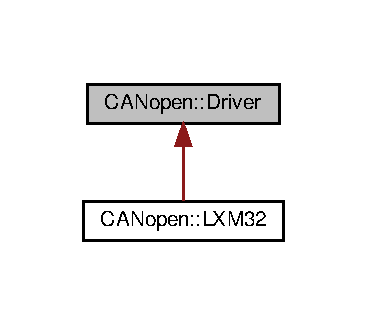
\includegraphics[width=176pt]{class_c_a_nopen_1_1_driver__inherit__graph}
\end{center}
\end{figure}
\subsection*{Public Types}
\begin{DoxyCompactItemize}
\item 
enum \hyperlink{class_c_a_nopen_1_1_driver_a9504ce08c5bec248880fe4e6803565f7}{Register} \+: uint32\+\_\+t \{ \newline
\hyperlink{class_c_a_nopen_1_1_driver_a9504ce08c5bec248880fe4e6803565f7a42423874643f633363c2ae56cac6f9b6}{Status\+Word} = 0x60410000, 
\hyperlink{class_c_a_nopen_1_1_driver_a9504ce08c5bec248880fe4e6803565f7ae4950e20abee18ade1ac2a03cb7da315}{Control\+Word} = 0x60400000, 
\hyperlink{class_c_a_nopen_1_1_driver_a9504ce08c5bec248880fe4e6803565f7a3999e1eaed36f6474242552c151d4053}{Op\+Mode} = 0x60600000, 
\hyperlink{class_c_a_nopen_1_1_driver_a9504ce08c5bec248880fe4e6803565f7a9388c18e3ec79d918b872aab89a47387}{P\+Pp\+\_\+target} = 0x607\+A0000, 
\newline
\hyperlink{class_c_a_nopen_1_1_driver_a9504ce08c5bec248880fe4e6803565f7a97069ba1c67700d01ba84c05f2a31adb}{P\+Pv\+\_\+target} = 0x60810000, 
\hyperlink{class_c_a_nopen_1_1_driver_a9504ce08c5bec248880fe4e6803565f7ae34a009131bb4956dbb9a5c9e76b1c5a}{R\+A\+M\+P\+\_\+v\+\_\+acc} = 0x60830000, 
\hyperlink{class_c_a_nopen_1_1_driver_a9504ce08c5bec248880fe4e6803565f7a6f355b7bef6158931cc8cf5e4b1f9c83}{R\+A\+M\+P\+\_\+v\+\_\+dec} = 0x60840000
 \}
\item 
enum \hyperlink{class_c_a_nopen_1_1_driver_af29fc14b8ec3ed982247a5129088a40f}{O\+Pmode} \+: uint8\+\_\+t \{ \hyperlink{class_c_a_nopen_1_1_driver_af29fc14b8ec3ed982247a5129088a40fa3502834b10b8f0201a628b9a0e227425}{Profile\+Position} = 1, 
\hyperlink{class_c_a_nopen_1_1_driver_af29fc14b8ec3ed982247a5129088a40fadb9f0017145112261254a48699a41961}{Profile\+Velocity} = 2
 \}
\item 
enum \hyperlink{class_c_a_nopen_1_1_driver_a16a451fc3593c0f174911e969a7be02d}{State} \+: uint16\+\_\+t \{ \newline
\hyperlink{class_c_a_nopen_1_1_driver_a16a451fc3593c0f174911e969a7be02da94d00ab583965d1d22f48674f7aefa7a}{Not\+Ready\+To\+Switcht\+ON} = 0x0000, 
\hyperlink{class_c_a_nopen_1_1_driver_a16a451fc3593c0f174911e969a7be02da868b030749591aa7b6afd1eade00edf7}{Switch\+On\+Disabled} = 0x0040, 
\hyperlink{class_c_a_nopen_1_1_driver_a16a451fc3593c0f174911e969a7be02dafa947edce547a30b314910e6931235a4}{Ready\+To\+Switch\+ON} = 0x0021, 
\hyperlink{class_c_a_nopen_1_1_driver_a16a451fc3593c0f174911e969a7be02dac2e13098b6500cdcde217d2a9cc9ebb6}{Switched\+ON} = 0x0023, 
\newline
\hyperlink{class_c_a_nopen_1_1_driver_a16a451fc3593c0f174911e969a7be02da1692c431e1cf20446dbf23a53913af0c}{Operation\+Enabled} = 0x0027, 
\hyperlink{class_c_a_nopen_1_1_driver_a16a451fc3593c0f174911e969a7be02da9028b5332c8352a087606c2cc79e9517}{Fault} = 0x000f, 
\hyperlink{class_c_a_nopen_1_1_driver_a16a451fc3593c0f174911e969a7be02dabafb33b6c4f43661a3257ca5b7569372}{Fault\+Reaction\+Active} = 0x000f, 
\hyperlink{class_c_a_nopen_1_1_driver_a16a451fc3593c0f174911e969a7be02da8accb6a0a36eebcd88f85e0b92faf68a}{Quick\+Stop\+Active} = 0x0007
 \}
\item 
enum \hyperlink{class_c_a_nopen_1_1_driver_af4031601d8ef94250316995e8339903a}{Control} \+: uint16\+\_\+t \{ \newline
\hyperlink{class_c_a_nopen_1_1_driver_af4031601d8ef94250316995e8339903aa6ccc4c2738c634abe2fd21cbe93f9fdb}{Shutdown} = 0x0006, 
\hyperlink{class_c_a_nopen_1_1_driver_af4031601d8ef94250316995e8339903aae98ed55dcd60bdd15d179ec32f651b8d}{Switch\+ON} = 0x0007, 
\hyperlink{class_c_a_nopen_1_1_driver_af4031601d8ef94250316995e8339903aa81c0fb39e9e145721e1cf45a52f8786f}{Disable\+Voltage} = 0x0000, 
\hyperlink{class_c_a_nopen_1_1_driver_af4031601d8ef94250316995e8339903aa6e8fc43d0b5f1ef14ac7ba475572c9b6}{Quick\+Stop} = 0x0002, 
\newline
\hyperlink{class_c_a_nopen_1_1_driver_af4031601d8ef94250316995e8339903aaa366dac5dbc508501f36112bf5472572}{Disable\+Operation} = 0x0007, 
\hyperlink{class_c_a_nopen_1_1_driver_af4031601d8ef94250316995e8339903aaff77b9045071e916120fc49e159d2f77}{Enable\+Operation} = 0x000f, 
\hyperlink{class_c_a_nopen_1_1_driver_af4031601d8ef94250316995e8339903aaa433113dfe71a54d4333344a339a9bbf}{Fault\+Resest} = 0x0080
 \}
\item 
enum \hyperlink{class_c_a_nopen_1_1_driver_af1538f81dbeb9dcafee3ff1a71c95be4}{P\+D\+O\+Function\+Code} \+: uint32\+\_\+t \{ \newline
\hyperlink{class_c_a_nopen_1_1_driver_af1538f81dbeb9dcafee3ff1a71c95be4aa31dc9b14e225c25d304e6d8d9b886ed}{P\+D\+O1\+Transmit} = Message\+:\+:P\+D\+O1\+Transmit, 
\hyperlink{class_c_a_nopen_1_1_driver_af1538f81dbeb9dcafee3ff1a71c95be4aa97a14880dee29baad7ee8201721c585}{P\+D\+O1\+Receive} = Message\+:\+:P\+D\+O1\+Receive, 
\hyperlink{class_c_a_nopen_1_1_driver_af1538f81dbeb9dcafee3ff1a71c95be4a013baa4e40e72d67279f8e5b5d9b4035}{P\+D\+O2\+Transmit} = Message\+:\+:P\+D\+O2\+Transmit, 
\hyperlink{class_c_a_nopen_1_1_driver_af1538f81dbeb9dcafee3ff1a71c95be4a9e3e5d76b75896fade4e2537f2e6e2f7}{P\+D\+O2\+Receive} = Message\+:\+:P\+D\+O2\+Receive, 
\newline
\hyperlink{class_c_a_nopen_1_1_driver_af1538f81dbeb9dcafee3ff1a71c95be4ae5889c8e1d945aa150ba4213617681d5}{P\+D\+O3\+Transmit} = Message\+:\+:P\+D\+O3\+Transmit, 
\hyperlink{class_c_a_nopen_1_1_driver_af1538f81dbeb9dcafee3ff1a71c95be4ad6ff06a6427b5f68ecea8552f1a01ef9}{P\+D\+O3\+Receive} = Message\+:\+:P\+D\+O3\+Receive, 
\hyperlink{class_c_a_nopen_1_1_driver_af1538f81dbeb9dcafee3ff1a71c95be4ae5f1f938d9d8b8833be74c805268e9ca}{P\+D\+O4\+Transmit} = Message\+:\+:P\+D\+O4\+Transmit, 
\hyperlink{class_c_a_nopen_1_1_driver_af1538f81dbeb9dcafee3ff1a71c95be4a6e9b86ade5180f6dcca330b94d1fd4da}{P\+D\+O4\+Receive} = Message\+:\+:P\+D\+O4\+Receive
 \}
\end{DoxyCompactItemize}
\subsection*{Public Member Functions}
\begin{DoxyCompactItemize}
\item 
\hyperlink{class_c_a_nopen_1_1_driver_a353dee2678e6049c216805dead97abfc}{Driver} (const char $\ast$ifname, uint16\+\_\+t can\+\_\+id, bool verbose=false)
\begin{DoxyCompactList}\small\item\em Constructor. \end{DoxyCompactList}\item 
bool \hyperlink{class_c_a_nopen_1_1_driver_a249f11262c9264cf53486c247d004b99}{is\+\_\+available} ()
\begin{DoxyCompactList}\small\item\em return true if the can interface is available \end{DoxyCompactList}\item 
void \hyperlink{class_c_a_nopen_1_1_driver_af549ce9c0b8c8125f8ddf26fab6810cf}{set\+\_\+\+P\+DO} (uint8\+\_\+t node\+\_\+id, \hyperlink{class_c_a_nopen_1_1_driver_af1538f81dbeb9dcafee3ff1a71c95be4}{P\+D\+O\+Function\+Code} fn)
\item 
void \hyperlink{class_c_a_nopen_1_1_driver_abd7d88699d02c007d5f23e608d8f0a0a}{stop} ()
\item 
void \hyperlink{class_c_a_nopen_1_1_driver_a35e035da9a3f9d6771f3e8b54ac80e73}{set\+\_\+mode} (int8\+\_\+t mode)
\item 
{\footnotesize template$<$typename T $>$ }\\void \hyperlink{class_c_a_nopen_1_1_driver_a66b64a600d9a0cdada81071b8cb412c8}{set} (\hyperlink{class_c_a_nopen_1_1_driver_a9504ce08c5bec248880fe4e6803565f7}{Register} reg, T param)
\item 
void \hyperlink{class_c_a_nopen_1_1_driver_ad82b69bd6c10c53ce4c7f766259ce804}{send\+\_\+\+P\+DO} (\hyperlink{class_c_a_nopen_1_1_driver_af1538f81dbeb9dcafee3ff1a71c95be4}{P\+D\+O\+Function\+Code} pdo, \hyperlink{class_c_a_nopen_1_1_payload}{Payload} payload)
\item 
void \hyperlink{class_c_a_nopen_1_1_driver_a2aab98740682098ccbfee1b8d3476c7a}{print\+\_\+status} ()
\item 
void \hyperlink{class_c_a_nopen_1_1_driver_a9bddeea1ccb9854c2b775248778903b5}{print\+\_\+control} ()
\end{DoxyCompactItemize}


\subsection{Detailed Description}


Definition at line 41 of file C\+A\+Nopen\+\_\+driver.\+h.



\subsection{Member Enumeration Documentation}
\mbox{\Hypertarget{class_c_a_nopen_1_1_driver_af4031601d8ef94250316995e8339903a}\label{class_c_a_nopen_1_1_driver_af4031601d8ef94250316995e8339903a}} 
\index{C\+A\+Nopen\+::\+Driver@{C\+A\+Nopen\+::\+Driver}!Control@{Control}}
\index{Control@{Control}!C\+A\+Nopen\+::\+Driver@{C\+A\+Nopen\+::\+Driver}}
\subsubsection{\texorpdfstring{Control}{Control}}
{\footnotesize\ttfamily enum \hyperlink{class_c_a_nopen_1_1_driver_af4031601d8ef94250316995e8339903a}{C\+A\+Nopen\+::\+Driver\+::\+Control} \+: uint16\+\_\+t}

Possible Control commands \begin{DoxyEnumFields}{Enumerator}
\raisebox{\heightof{T}}[0pt][0pt]{\index{Shutdown@{Shutdown}!C\+A\+Nopen\+::\+Driver@{C\+A\+Nopen\+::\+Driver}}\index{C\+A\+Nopen\+::\+Driver@{C\+A\+Nopen\+::\+Driver}!Shutdown@{Shutdown}}}\mbox{\Hypertarget{class_c_a_nopen_1_1_driver_af4031601d8ef94250316995e8339903aa6ccc4c2738c634abe2fd21cbe93f9fdb}\label{class_c_a_nopen_1_1_driver_af4031601d8ef94250316995e8339903aa6ccc4c2738c634abe2fd21cbe93f9fdb}} 
Shutdown&goto Ready\+Switch\+ON \\
\hline

\raisebox{\heightof{T}}[0pt][0pt]{\index{Switch\+ON@{Switch\+ON}!C\+A\+Nopen\+::\+Driver@{C\+A\+Nopen\+::\+Driver}}\index{C\+A\+Nopen\+::\+Driver@{C\+A\+Nopen\+::\+Driver}!Switch\+ON@{Switch\+ON}}}\mbox{\Hypertarget{class_c_a_nopen_1_1_driver_af4031601d8ef94250316995e8339903aae98ed55dcd60bdd15d179ec32f651b8d}\label{class_c_a_nopen_1_1_driver_af4031601d8ef94250316995e8339903aae98ed55dcd60bdd15d179ec32f651b8d}} 
Switch\+ON&goto Switched\+ON \\
\hline

\raisebox{\heightof{T}}[0pt][0pt]{\index{Disable\+Voltage@{Disable\+Voltage}!C\+A\+Nopen\+::\+Driver@{C\+A\+Nopen\+::\+Driver}}\index{C\+A\+Nopen\+::\+Driver@{C\+A\+Nopen\+::\+Driver}!Disable\+Voltage@{Disable\+Voltage}}}\mbox{\Hypertarget{class_c_a_nopen_1_1_driver_af4031601d8ef94250316995e8339903aa81c0fb39e9e145721e1cf45a52f8786f}\label{class_c_a_nopen_1_1_driver_af4031601d8ef94250316995e8339903aa81c0fb39e9e145721e1cf45a52f8786f}} 
Disable\+Voltage&goto Switch\+O\+N\+Disabled \\
\hline

\raisebox{\heightof{T}}[0pt][0pt]{\index{Quick\+Stop@{Quick\+Stop}!C\+A\+Nopen\+::\+Driver@{C\+A\+Nopen\+::\+Driver}}\index{C\+A\+Nopen\+::\+Driver@{C\+A\+Nopen\+::\+Driver}!Quick\+Stop@{Quick\+Stop}}}\mbox{\Hypertarget{class_c_a_nopen_1_1_driver_af4031601d8ef94250316995e8339903aa6e8fc43d0b5f1ef14ac7ba475572c9b6}\label{class_c_a_nopen_1_1_driver_af4031601d8ef94250316995e8339903aa6e8fc43d0b5f1ef14ac7ba475572c9b6}} 
Quick\+Stop&goto Quick\+Stop\+Activ \\
\hline

\raisebox{\heightof{T}}[0pt][0pt]{\index{Disable\+Operation@{Disable\+Operation}!C\+A\+Nopen\+::\+Driver@{C\+A\+Nopen\+::\+Driver}}\index{C\+A\+Nopen\+::\+Driver@{C\+A\+Nopen\+::\+Driver}!Disable\+Operation@{Disable\+Operation}}}\mbox{\Hypertarget{class_c_a_nopen_1_1_driver_af4031601d8ef94250316995e8339903aaa366dac5dbc508501f36112bf5472572}\label{class_c_a_nopen_1_1_driver_af4031601d8ef94250316995e8339903aaa366dac5dbc508501f36112bf5472572}} 
Disable\+Operation&goto Switched\+ON \\
\hline

\raisebox{\heightof{T}}[0pt][0pt]{\index{Enable\+Operation@{Enable\+Operation}!C\+A\+Nopen\+::\+Driver@{C\+A\+Nopen\+::\+Driver}}\index{C\+A\+Nopen\+::\+Driver@{C\+A\+Nopen\+::\+Driver}!Enable\+Operation@{Enable\+Operation}}}\mbox{\Hypertarget{class_c_a_nopen_1_1_driver_af4031601d8ef94250316995e8339903aaff77b9045071e916120fc49e159d2f77}\label{class_c_a_nopen_1_1_driver_af4031601d8ef94250316995e8339903aaff77b9045071e916120fc49e159d2f77}} 
Enable\+Operation&goto Operation\+Enabled \\
\hline

\raisebox{\heightof{T}}[0pt][0pt]{\index{Fault\+Resest@{Fault\+Resest}!C\+A\+Nopen\+::\+Driver@{C\+A\+Nopen\+::\+Driver}}\index{C\+A\+Nopen\+::\+Driver@{C\+A\+Nopen\+::\+Driver}!Fault\+Resest@{Fault\+Resest}}}\mbox{\Hypertarget{class_c_a_nopen_1_1_driver_af4031601d8ef94250316995e8339903aaa433113dfe71a54d4333344a339a9bbf}\label{class_c_a_nopen_1_1_driver_af4031601d8ef94250316995e8339903aaa433113dfe71a54d4333344a339a9bbf}} 
Fault\+Resest&goto Switch\+O\+N\+Disabled \\
\hline

\end{DoxyEnumFields}


Definition at line 75 of file C\+A\+Nopen\+\_\+driver.\+h.

\mbox{\Hypertarget{class_c_a_nopen_1_1_driver_af29fc14b8ec3ed982247a5129088a40f}\label{class_c_a_nopen_1_1_driver_af29fc14b8ec3ed982247a5129088a40f}} 
\index{C\+A\+Nopen\+::\+Driver@{C\+A\+Nopen\+::\+Driver}!O\+Pmode@{O\+Pmode}}
\index{O\+Pmode@{O\+Pmode}!C\+A\+Nopen\+::\+Driver@{C\+A\+Nopen\+::\+Driver}}
\subsubsection{\texorpdfstring{O\+Pmode}{OPmode}}
{\footnotesize\ttfamily enum \hyperlink{class_c_a_nopen_1_1_driver_af29fc14b8ec3ed982247a5129088a40f}{C\+A\+Nopen\+::\+Driver\+::\+O\+Pmode} \+: uint8\+\_\+t}

\begin{DoxyEnumFields}{Enumerator}
\raisebox{\heightof{T}}[0pt][0pt]{\index{Profile\+Position@{Profile\+Position}!C\+A\+Nopen\+::\+Driver@{C\+A\+Nopen\+::\+Driver}}\index{C\+A\+Nopen\+::\+Driver@{C\+A\+Nopen\+::\+Driver}!Profile\+Position@{Profile\+Position}}}\mbox{\Hypertarget{class_c_a_nopen_1_1_driver_af29fc14b8ec3ed982247a5129088a40fa3502834b10b8f0201a628b9a0e227425}\label{class_c_a_nopen_1_1_driver_af29fc14b8ec3ed982247a5129088a40fa3502834b10b8f0201a628b9a0e227425}} 
Profile\+Position&\\
\hline

\raisebox{\heightof{T}}[0pt][0pt]{\index{Profile\+Velocity@{Profile\+Velocity}!C\+A\+Nopen\+::\+Driver@{C\+A\+Nopen\+::\+Driver}}\index{C\+A\+Nopen\+::\+Driver@{C\+A\+Nopen\+::\+Driver}!Profile\+Velocity@{Profile\+Velocity}}}\mbox{\Hypertarget{class_c_a_nopen_1_1_driver_af29fc14b8ec3ed982247a5129088a40fadb9f0017145112261254a48699a41961}\label{class_c_a_nopen_1_1_driver_af29fc14b8ec3ed982247a5129088a40fadb9f0017145112261254a48699a41961}} 
Profile\+Velocity&\\
\hline

\end{DoxyEnumFields}


Definition at line 53 of file C\+A\+Nopen\+\_\+driver.\+h.

\mbox{\Hypertarget{class_c_a_nopen_1_1_driver_af1538f81dbeb9dcafee3ff1a71c95be4}\label{class_c_a_nopen_1_1_driver_af1538f81dbeb9dcafee3ff1a71c95be4}} 
\index{C\+A\+Nopen\+::\+Driver@{C\+A\+Nopen\+::\+Driver}!P\+D\+O\+Function\+Code@{P\+D\+O\+Function\+Code}}
\index{P\+D\+O\+Function\+Code@{P\+D\+O\+Function\+Code}!C\+A\+Nopen\+::\+Driver@{C\+A\+Nopen\+::\+Driver}}
\subsubsection{\texorpdfstring{P\+D\+O\+Function\+Code}{PDOFunctionCode}}
{\footnotesize\ttfamily enum \hyperlink{class_c_a_nopen_1_1_driver_af1538f81dbeb9dcafee3ff1a71c95be4}{C\+A\+Nopen\+::\+Driver\+::\+P\+D\+O\+Function\+Code} \+: uint32\+\_\+t}

\begin{DoxyEnumFields}{Enumerator}
\raisebox{\heightof{T}}[0pt][0pt]{\index{P\+D\+O1\+Transmit@{P\+D\+O1\+Transmit}!C\+A\+Nopen\+::\+Driver@{C\+A\+Nopen\+::\+Driver}}\index{C\+A\+Nopen\+::\+Driver@{C\+A\+Nopen\+::\+Driver}!P\+D\+O1\+Transmit@{P\+D\+O1\+Transmit}}}\mbox{\Hypertarget{class_c_a_nopen_1_1_driver_af1538f81dbeb9dcafee3ff1a71c95be4aa31dc9b14e225c25d304e6d8d9b886ed}\label{class_c_a_nopen_1_1_driver_af1538f81dbeb9dcafee3ff1a71c95be4aa31dc9b14e225c25d304e6d8d9b886ed}} 
P\+D\+O1\+Transmit&\\
\hline

\raisebox{\heightof{T}}[0pt][0pt]{\index{P\+D\+O1\+Receive@{P\+D\+O1\+Receive}!C\+A\+Nopen\+::\+Driver@{C\+A\+Nopen\+::\+Driver}}\index{C\+A\+Nopen\+::\+Driver@{C\+A\+Nopen\+::\+Driver}!P\+D\+O1\+Receive@{P\+D\+O1\+Receive}}}\mbox{\Hypertarget{class_c_a_nopen_1_1_driver_af1538f81dbeb9dcafee3ff1a71c95be4aa97a14880dee29baad7ee8201721c585}\label{class_c_a_nopen_1_1_driver_af1538f81dbeb9dcafee3ff1a71c95be4aa97a14880dee29baad7ee8201721c585}} 
P\+D\+O1\+Receive&\\
\hline

\raisebox{\heightof{T}}[0pt][0pt]{\index{P\+D\+O2\+Transmit@{P\+D\+O2\+Transmit}!C\+A\+Nopen\+::\+Driver@{C\+A\+Nopen\+::\+Driver}}\index{C\+A\+Nopen\+::\+Driver@{C\+A\+Nopen\+::\+Driver}!P\+D\+O2\+Transmit@{P\+D\+O2\+Transmit}}}\mbox{\Hypertarget{class_c_a_nopen_1_1_driver_af1538f81dbeb9dcafee3ff1a71c95be4a013baa4e40e72d67279f8e5b5d9b4035}\label{class_c_a_nopen_1_1_driver_af1538f81dbeb9dcafee3ff1a71c95be4a013baa4e40e72d67279f8e5b5d9b4035}} 
P\+D\+O2\+Transmit&\\
\hline

\raisebox{\heightof{T}}[0pt][0pt]{\index{P\+D\+O2\+Receive@{P\+D\+O2\+Receive}!C\+A\+Nopen\+::\+Driver@{C\+A\+Nopen\+::\+Driver}}\index{C\+A\+Nopen\+::\+Driver@{C\+A\+Nopen\+::\+Driver}!P\+D\+O2\+Receive@{P\+D\+O2\+Receive}}}\mbox{\Hypertarget{class_c_a_nopen_1_1_driver_af1538f81dbeb9dcafee3ff1a71c95be4a9e3e5d76b75896fade4e2537f2e6e2f7}\label{class_c_a_nopen_1_1_driver_af1538f81dbeb9dcafee3ff1a71c95be4a9e3e5d76b75896fade4e2537f2e6e2f7}} 
P\+D\+O2\+Receive&\\
\hline

\raisebox{\heightof{T}}[0pt][0pt]{\index{P\+D\+O3\+Transmit@{P\+D\+O3\+Transmit}!C\+A\+Nopen\+::\+Driver@{C\+A\+Nopen\+::\+Driver}}\index{C\+A\+Nopen\+::\+Driver@{C\+A\+Nopen\+::\+Driver}!P\+D\+O3\+Transmit@{P\+D\+O3\+Transmit}}}\mbox{\Hypertarget{class_c_a_nopen_1_1_driver_af1538f81dbeb9dcafee3ff1a71c95be4ae5889c8e1d945aa150ba4213617681d5}\label{class_c_a_nopen_1_1_driver_af1538f81dbeb9dcafee3ff1a71c95be4ae5889c8e1d945aa150ba4213617681d5}} 
P\+D\+O3\+Transmit&\\
\hline

\raisebox{\heightof{T}}[0pt][0pt]{\index{P\+D\+O3\+Receive@{P\+D\+O3\+Receive}!C\+A\+Nopen\+::\+Driver@{C\+A\+Nopen\+::\+Driver}}\index{C\+A\+Nopen\+::\+Driver@{C\+A\+Nopen\+::\+Driver}!P\+D\+O3\+Receive@{P\+D\+O3\+Receive}}}\mbox{\Hypertarget{class_c_a_nopen_1_1_driver_af1538f81dbeb9dcafee3ff1a71c95be4ad6ff06a6427b5f68ecea8552f1a01ef9}\label{class_c_a_nopen_1_1_driver_af1538f81dbeb9dcafee3ff1a71c95be4ad6ff06a6427b5f68ecea8552f1a01ef9}} 
P\+D\+O3\+Receive&\\
\hline

\raisebox{\heightof{T}}[0pt][0pt]{\index{P\+D\+O4\+Transmit@{P\+D\+O4\+Transmit}!C\+A\+Nopen\+::\+Driver@{C\+A\+Nopen\+::\+Driver}}\index{C\+A\+Nopen\+::\+Driver@{C\+A\+Nopen\+::\+Driver}!P\+D\+O4\+Transmit@{P\+D\+O4\+Transmit}}}\mbox{\Hypertarget{class_c_a_nopen_1_1_driver_af1538f81dbeb9dcafee3ff1a71c95be4ae5f1f938d9d8b8833be74c805268e9ca}\label{class_c_a_nopen_1_1_driver_af1538f81dbeb9dcafee3ff1a71c95be4ae5f1f938d9d8b8833be74c805268e9ca}} 
P\+D\+O4\+Transmit&\\
\hline

\raisebox{\heightof{T}}[0pt][0pt]{\index{P\+D\+O4\+Receive@{P\+D\+O4\+Receive}!C\+A\+Nopen\+::\+Driver@{C\+A\+Nopen\+::\+Driver}}\index{C\+A\+Nopen\+::\+Driver@{C\+A\+Nopen\+::\+Driver}!P\+D\+O4\+Receive@{P\+D\+O4\+Receive}}}\mbox{\Hypertarget{class_c_a_nopen_1_1_driver_af1538f81dbeb9dcafee3ff1a71c95be4a6e9b86ade5180f6dcca330b94d1fd4da}\label{class_c_a_nopen_1_1_driver_af1538f81dbeb9dcafee3ff1a71c95be4a6e9b86ade5180f6dcca330b94d1fd4da}} 
P\+D\+O4\+Receive&\\
\hline

\end{DoxyEnumFields}


Definition at line 85 of file C\+A\+Nopen\+\_\+driver.\+h.

\mbox{\Hypertarget{class_c_a_nopen_1_1_driver_a9504ce08c5bec248880fe4e6803565f7}\label{class_c_a_nopen_1_1_driver_a9504ce08c5bec248880fe4e6803565f7}} 
\index{C\+A\+Nopen\+::\+Driver@{C\+A\+Nopen\+::\+Driver}!Register@{Register}}
\index{Register@{Register}!C\+A\+Nopen\+::\+Driver@{C\+A\+Nopen\+::\+Driver}}
\subsubsection{\texorpdfstring{Register}{Register}}
{\footnotesize\ttfamily enum \hyperlink{class_c_a_nopen_1_1_driver_a9504ce08c5bec248880fe4e6803565f7}{C\+A\+Nopen\+::\+Driver\+::\+Register} \+: uint32\+\_\+t}

\begin{DoxyEnumFields}{Enumerator}
\raisebox{\heightof{T}}[0pt][0pt]{\index{Status\+Word@{Status\+Word}!C\+A\+Nopen\+::\+Driver@{C\+A\+Nopen\+::\+Driver}}\index{C\+A\+Nopen\+::\+Driver@{C\+A\+Nopen\+::\+Driver}!Status\+Word@{Status\+Word}}}\mbox{\Hypertarget{class_c_a_nopen_1_1_driver_a9504ce08c5bec248880fe4e6803565f7a42423874643f633363c2ae56cac6f9b6}\label{class_c_a_nopen_1_1_driver_a9504ce08c5bec248880fe4e6803565f7a42423874643f633363c2ae56cac6f9b6}} 
Status\+Word&\\
\hline

\raisebox{\heightof{T}}[0pt][0pt]{\index{Control\+Word@{Control\+Word}!C\+A\+Nopen\+::\+Driver@{C\+A\+Nopen\+::\+Driver}}\index{C\+A\+Nopen\+::\+Driver@{C\+A\+Nopen\+::\+Driver}!Control\+Word@{Control\+Word}}}\mbox{\Hypertarget{class_c_a_nopen_1_1_driver_a9504ce08c5bec248880fe4e6803565f7ae4950e20abee18ade1ac2a03cb7da315}\label{class_c_a_nopen_1_1_driver_a9504ce08c5bec248880fe4e6803565f7ae4950e20abee18ade1ac2a03cb7da315}} 
Control\+Word&\\
\hline

\raisebox{\heightof{T}}[0pt][0pt]{\index{Op\+Mode@{Op\+Mode}!C\+A\+Nopen\+::\+Driver@{C\+A\+Nopen\+::\+Driver}}\index{C\+A\+Nopen\+::\+Driver@{C\+A\+Nopen\+::\+Driver}!Op\+Mode@{Op\+Mode}}}\mbox{\Hypertarget{class_c_a_nopen_1_1_driver_a9504ce08c5bec248880fe4e6803565f7a3999e1eaed36f6474242552c151d4053}\label{class_c_a_nopen_1_1_driver_a9504ce08c5bec248880fe4e6803565f7a3999e1eaed36f6474242552c151d4053}} 
Op\+Mode&\\
\hline

\raisebox{\heightof{T}}[0pt][0pt]{\index{P\+Pp\+\_\+target@{P\+Pp\+\_\+target}!C\+A\+Nopen\+::\+Driver@{C\+A\+Nopen\+::\+Driver}}\index{C\+A\+Nopen\+::\+Driver@{C\+A\+Nopen\+::\+Driver}!P\+Pp\+\_\+target@{P\+Pp\+\_\+target}}}\mbox{\Hypertarget{class_c_a_nopen_1_1_driver_a9504ce08c5bec248880fe4e6803565f7a9388c18e3ec79d918b872aab89a47387}\label{class_c_a_nopen_1_1_driver_a9504ce08c5bec248880fe4e6803565f7a9388c18e3ec79d918b872aab89a47387}} 
P\+Pp\+\_\+target&\\
\hline

\raisebox{\heightof{T}}[0pt][0pt]{\index{P\+Pv\+\_\+target@{P\+Pv\+\_\+target}!C\+A\+Nopen\+::\+Driver@{C\+A\+Nopen\+::\+Driver}}\index{C\+A\+Nopen\+::\+Driver@{C\+A\+Nopen\+::\+Driver}!P\+Pv\+\_\+target@{P\+Pv\+\_\+target}}}\mbox{\Hypertarget{class_c_a_nopen_1_1_driver_a9504ce08c5bec248880fe4e6803565f7a97069ba1c67700d01ba84c05f2a31adb}\label{class_c_a_nopen_1_1_driver_a9504ce08c5bec248880fe4e6803565f7a97069ba1c67700d01ba84c05f2a31adb}} 
P\+Pv\+\_\+target&\\
\hline

\raisebox{\heightof{T}}[0pt][0pt]{\index{R\+A\+M\+P\+\_\+v\+\_\+acc@{R\+A\+M\+P\+\_\+v\+\_\+acc}!C\+A\+Nopen\+::\+Driver@{C\+A\+Nopen\+::\+Driver}}\index{C\+A\+Nopen\+::\+Driver@{C\+A\+Nopen\+::\+Driver}!R\+A\+M\+P\+\_\+v\+\_\+acc@{R\+A\+M\+P\+\_\+v\+\_\+acc}}}\mbox{\Hypertarget{class_c_a_nopen_1_1_driver_a9504ce08c5bec248880fe4e6803565f7ae34a009131bb4956dbb9a5c9e76b1c5a}\label{class_c_a_nopen_1_1_driver_a9504ce08c5bec248880fe4e6803565f7ae34a009131bb4956dbb9a5c9e76b1c5a}} 
R\+A\+M\+P\+\_\+v\+\_\+acc&\\
\hline

\raisebox{\heightof{T}}[0pt][0pt]{\index{R\+A\+M\+P\+\_\+v\+\_\+dec@{R\+A\+M\+P\+\_\+v\+\_\+dec}!C\+A\+Nopen\+::\+Driver@{C\+A\+Nopen\+::\+Driver}}\index{C\+A\+Nopen\+::\+Driver@{C\+A\+Nopen\+::\+Driver}!R\+A\+M\+P\+\_\+v\+\_\+dec@{R\+A\+M\+P\+\_\+v\+\_\+dec}}}\mbox{\Hypertarget{class_c_a_nopen_1_1_driver_a9504ce08c5bec248880fe4e6803565f7a6f355b7bef6158931cc8cf5e4b1f9c83}\label{class_c_a_nopen_1_1_driver_a9504ce08c5bec248880fe4e6803565f7a6f355b7bef6158931cc8cf5e4b1f9c83}} 
R\+A\+M\+P\+\_\+v\+\_\+dec&\\
\hline

\end{DoxyEnumFields}


Definition at line 43 of file C\+A\+Nopen\+\_\+driver.\+h.

\mbox{\Hypertarget{class_c_a_nopen_1_1_driver_a16a451fc3593c0f174911e969a7be02d}\label{class_c_a_nopen_1_1_driver_a16a451fc3593c0f174911e969a7be02d}} 
\index{C\+A\+Nopen\+::\+Driver@{C\+A\+Nopen\+::\+Driver}!State@{State}}
\index{State@{State}!C\+A\+Nopen\+::\+Driver@{C\+A\+Nopen\+::\+Driver}}
\subsubsection{\texorpdfstring{State}{State}}
{\footnotesize\ttfamily enum \hyperlink{class_c_a_nopen_1_1_driver_a16a451fc3593c0f174911e969a7be02d}{C\+A\+Nopen\+::\+Driver\+::\+State} \+: uint16\+\_\+t}

Possible States \begin{DoxyEnumFields}{Enumerator}
\raisebox{\heightof{T}}[0pt][0pt]{\index{Not\+Ready\+To\+Switcht\+ON@{Not\+Ready\+To\+Switcht\+ON}!C\+A\+Nopen\+::\+Driver@{C\+A\+Nopen\+::\+Driver}}\index{C\+A\+Nopen\+::\+Driver@{C\+A\+Nopen\+::\+Driver}!Not\+Ready\+To\+Switcht\+ON@{Not\+Ready\+To\+Switcht\+ON}}}\mbox{\Hypertarget{class_c_a_nopen_1_1_driver_a16a451fc3593c0f174911e969a7be02da94d00ab583965d1d22f48674f7aefa7a}\label{class_c_a_nopen_1_1_driver_a16a451fc3593c0f174911e969a7be02da94d00ab583965d1d22f48674f7aefa7a}} 
Not\+Ready\+To\+Switcht\+ON&Not Ready to Switch ON\+:
\begin{DoxyItemize}
\item Low level Power (e.\+g. 15V, 5V) has been applied to the drive.
\item The drive is being initialized or is running self test.
\item A brake, if present, has to be applied in this state.
\item The drive function is disabled. 
\end{DoxyItemize}\\
\hline

\raisebox{\heightof{T}}[0pt][0pt]{\index{Switch\+On\+Disabled@{Switch\+On\+Disabled}!C\+A\+Nopen\+::\+Driver@{C\+A\+Nopen\+::\+Driver}}\index{C\+A\+Nopen\+::\+Driver@{C\+A\+Nopen\+::\+Driver}!Switch\+On\+Disabled@{Switch\+On\+Disabled}}}\mbox{\Hypertarget{class_c_a_nopen_1_1_driver_a16a451fc3593c0f174911e969a7be02da868b030749591aa7b6afd1eade00edf7}\label{class_c_a_nopen_1_1_driver_a16a451fc3593c0f174911e969a7be02da868b030749591aa7b6afd1eade00edf7}} 
Switch\+On\+Disabled&\\
\hline

\raisebox{\heightof{T}}[0pt][0pt]{\index{Ready\+To\+Switch\+ON@{Ready\+To\+Switch\+ON}!C\+A\+Nopen\+::\+Driver@{C\+A\+Nopen\+::\+Driver}}\index{C\+A\+Nopen\+::\+Driver@{C\+A\+Nopen\+::\+Driver}!Ready\+To\+Switch\+ON@{Ready\+To\+Switch\+ON}}}\mbox{\Hypertarget{class_c_a_nopen_1_1_driver_a16a451fc3593c0f174911e969a7be02dafa947edce547a30b314910e6931235a4}\label{class_c_a_nopen_1_1_driver_a16a451fc3593c0f174911e969a7be02dafa947edce547a30b314910e6931235a4}} 
Ready\+To\+Switch\+ON&\\
\hline

\raisebox{\heightof{T}}[0pt][0pt]{\index{Switched\+ON@{Switched\+ON}!C\+A\+Nopen\+::\+Driver@{C\+A\+Nopen\+::\+Driver}}\index{C\+A\+Nopen\+::\+Driver@{C\+A\+Nopen\+::\+Driver}!Switched\+ON@{Switched\+ON}}}\mbox{\Hypertarget{class_c_a_nopen_1_1_driver_a16a451fc3593c0f174911e969a7be02dac2e13098b6500cdcde217d2a9cc9ebb6}\label{class_c_a_nopen_1_1_driver_a16a451fc3593c0f174911e969a7be02dac2e13098b6500cdcde217d2a9cc9ebb6}} 
Switched\+ON&\\
\hline

\raisebox{\heightof{T}}[0pt][0pt]{\index{Operation\+Enabled@{Operation\+Enabled}!C\+A\+Nopen\+::\+Driver@{C\+A\+Nopen\+::\+Driver}}\index{C\+A\+Nopen\+::\+Driver@{C\+A\+Nopen\+::\+Driver}!Operation\+Enabled@{Operation\+Enabled}}}\mbox{\Hypertarget{class_c_a_nopen_1_1_driver_a16a451fc3593c0f174911e969a7be02da1692c431e1cf20446dbf23a53913af0c}\label{class_c_a_nopen_1_1_driver_a16a451fc3593c0f174911e969a7be02da1692c431e1cf20446dbf23a53913af0c}} 
Operation\+Enabled&\\
\hline

\raisebox{\heightof{T}}[0pt][0pt]{\index{Fault@{Fault}!C\+A\+Nopen\+::\+Driver@{C\+A\+Nopen\+::\+Driver}}\index{C\+A\+Nopen\+::\+Driver@{C\+A\+Nopen\+::\+Driver}!Fault@{Fault}}}\mbox{\Hypertarget{class_c_a_nopen_1_1_driver_a16a451fc3593c0f174911e969a7be02da9028b5332c8352a087606c2cc79e9517}\label{class_c_a_nopen_1_1_driver_a16a451fc3593c0f174911e969a7be02da9028b5332c8352a087606c2cc79e9517}} 
Fault&\\
\hline

\raisebox{\heightof{T}}[0pt][0pt]{\index{Fault\+Reaction\+Active@{Fault\+Reaction\+Active}!C\+A\+Nopen\+::\+Driver@{C\+A\+Nopen\+::\+Driver}}\index{C\+A\+Nopen\+::\+Driver@{C\+A\+Nopen\+::\+Driver}!Fault\+Reaction\+Active@{Fault\+Reaction\+Active}}}\mbox{\Hypertarget{class_c_a_nopen_1_1_driver_a16a451fc3593c0f174911e969a7be02dabafb33b6c4f43661a3257ca5b7569372}\label{class_c_a_nopen_1_1_driver_a16a451fc3593c0f174911e969a7be02dabafb33b6c4f43661a3257ca5b7569372}} 
Fault\+Reaction\+Active&\\
\hline

\raisebox{\heightof{T}}[0pt][0pt]{\index{Quick\+Stop\+Active@{Quick\+Stop\+Active}!C\+A\+Nopen\+::\+Driver@{C\+A\+Nopen\+::\+Driver}}\index{C\+A\+Nopen\+::\+Driver@{C\+A\+Nopen\+::\+Driver}!Quick\+Stop\+Active@{Quick\+Stop\+Active}}}\mbox{\Hypertarget{class_c_a_nopen_1_1_driver_a16a451fc3593c0f174911e969a7be02da8accb6a0a36eebcd88f85e0b92faf68a}\label{class_c_a_nopen_1_1_driver_a16a451fc3593c0f174911e969a7be02da8accb6a0a36eebcd88f85e0b92faf68a}} 
Quick\+Stop\+Active&\\
\hline

\end{DoxyEnumFields}


Definition at line 59 of file C\+A\+Nopen\+\_\+driver.\+h.



\subsection{Constructor \& Destructor Documentation}
\mbox{\Hypertarget{class_c_a_nopen_1_1_driver_a353dee2678e6049c216805dead97abfc}\label{class_c_a_nopen_1_1_driver_a353dee2678e6049c216805dead97abfc}} 
\index{C\+A\+Nopen\+::\+Driver@{C\+A\+Nopen\+::\+Driver}!Driver@{Driver}}
\index{Driver@{Driver}!C\+A\+Nopen\+::\+Driver@{C\+A\+Nopen\+::\+Driver}}
\subsubsection{\texorpdfstring{Driver()}{Driver()}}
{\footnotesize\ttfamily C\+A\+Nopen\+::\+Driver\+::\+Driver (\begin{DoxyParamCaption}\item[{const char $\ast$}]{ifname,  }\item[{uint16\+\_\+t}]{can\+\_\+id,  }\item[{bool}]{verbose = {\ttfamily false} }\end{DoxyParamCaption})}



Constructor. 


\begin{DoxyParams}{Parameters}
{\em ifname} & \+: Name of the C\+AN interface. \\
\hline
{\em can\+\_\+id} & \+: Node C\+AN ID of the driver. \\
\hline
\end{DoxyParams}


Definition at line 3 of file C\+A\+Nopen\+\_\+driver.\+cpp.



\subsection{Member Function Documentation}
\mbox{\Hypertarget{class_c_a_nopen_1_1_driver_a249f11262c9264cf53486c247d004b99}\label{class_c_a_nopen_1_1_driver_a249f11262c9264cf53486c247d004b99}} 
\index{C\+A\+Nopen\+::\+Driver@{C\+A\+Nopen\+::\+Driver}!is\+\_\+available@{is\+\_\+available}}
\index{is\+\_\+available@{is\+\_\+available}!C\+A\+Nopen\+::\+Driver@{C\+A\+Nopen\+::\+Driver}}
\subsubsection{\texorpdfstring{is\+\_\+available()}{is\_available()}}
{\footnotesize\ttfamily bool C\+A\+Nopen\+::\+Driver\+::is\+\_\+available (\begin{DoxyParamCaption}{ }\end{DoxyParamCaption})\hspace{0.3cm}{\ttfamily [inline]}}



return true if the can interface is available 



Definition at line 106 of file C\+A\+Nopen\+\_\+driver.\+h.

\mbox{\Hypertarget{class_c_a_nopen_1_1_driver_a9bddeea1ccb9854c2b775248778903b5}\label{class_c_a_nopen_1_1_driver_a9bddeea1ccb9854c2b775248778903b5}} 
\index{C\+A\+Nopen\+::\+Driver@{C\+A\+Nopen\+::\+Driver}!print\+\_\+control@{print\+\_\+control}}
\index{print\+\_\+control@{print\+\_\+control}!C\+A\+Nopen\+::\+Driver@{C\+A\+Nopen\+::\+Driver}}
\subsubsection{\texorpdfstring{print\+\_\+control()}{print\_control()}}
{\footnotesize\ttfamily void C\+A\+Nopen\+::\+Driver\+::print\+\_\+control (\begin{DoxyParamCaption}{ }\end{DoxyParamCaption})}



Definition at line 109 of file C\+A\+Nopen\+\_\+driver.\+cpp.

\mbox{\Hypertarget{class_c_a_nopen_1_1_driver_a2aab98740682098ccbfee1b8d3476c7a}\label{class_c_a_nopen_1_1_driver_a2aab98740682098ccbfee1b8d3476c7a}} 
\index{C\+A\+Nopen\+::\+Driver@{C\+A\+Nopen\+::\+Driver}!print\+\_\+status@{print\+\_\+status}}
\index{print\+\_\+status@{print\+\_\+status}!C\+A\+Nopen\+::\+Driver@{C\+A\+Nopen\+::\+Driver}}
\subsubsection{\texorpdfstring{print\+\_\+status()}{print\_status()}}
{\footnotesize\ttfamily void C\+A\+Nopen\+::\+Driver\+::print\+\_\+status (\begin{DoxyParamCaption}{ }\end{DoxyParamCaption})}



Definition at line 52 of file C\+A\+Nopen\+\_\+driver.\+cpp.

\mbox{\Hypertarget{class_c_a_nopen_1_1_driver_ad82b69bd6c10c53ce4c7f766259ce804}\label{class_c_a_nopen_1_1_driver_ad82b69bd6c10c53ce4c7f766259ce804}} 
\index{C\+A\+Nopen\+::\+Driver@{C\+A\+Nopen\+::\+Driver}!send\+\_\+\+P\+DO@{send\+\_\+\+P\+DO}}
\index{send\+\_\+\+P\+DO@{send\+\_\+\+P\+DO}!C\+A\+Nopen\+::\+Driver@{C\+A\+Nopen\+::\+Driver}}
\subsubsection{\texorpdfstring{send\+\_\+\+P\+D\+O()}{send\_PDO()}}
{\footnotesize\ttfamily void C\+A\+Nopen\+::\+Driver\+::send\+\_\+\+P\+DO (\begin{DoxyParamCaption}\item[{\hyperlink{class_c_a_nopen_1_1_driver_af1538f81dbeb9dcafee3ff1a71c95be4}{P\+D\+O\+Function\+Code}}]{pdo,  }\item[{\hyperlink{class_c_a_nopen_1_1_payload}{Payload}}]{payload }\end{DoxyParamCaption})}



Definition at line 36 of file C\+A\+Nopen\+\_\+driver.\+cpp.

\mbox{\Hypertarget{class_c_a_nopen_1_1_driver_a66b64a600d9a0cdada81071b8cb412c8}\label{class_c_a_nopen_1_1_driver_a66b64a600d9a0cdada81071b8cb412c8}} 
\index{C\+A\+Nopen\+::\+Driver@{C\+A\+Nopen\+::\+Driver}!set@{set}}
\index{set@{set}!C\+A\+Nopen\+::\+Driver@{C\+A\+Nopen\+::\+Driver}}
\subsubsection{\texorpdfstring{set()}{set()}}
{\footnotesize\ttfamily template$<$typename T $>$ \\
void C\+A\+Nopen\+::\+Driver\+::set (\begin{DoxyParamCaption}\item[{\hyperlink{class_c_a_nopen_1_1_driver_a9504ce08c5bec248880fe4e6803565f7}{Register}}]{reg,  }\item[{T}]{param }\end{DoxyParamCaption})\hspace{0.3cm}{\ttfamily [inline]}}



Definition at line 122 of file C\+A\+Nopen\+\_\+driver.\+h.

\mbox{\Hypertarget{class_c_a_nopen_1_1_driver_a35e035da9a3f9d6771f3e8b54ac80e73}\label{class_c_a_nopen_1_1_driver_a35e035da9a3f9d6771f3e8b54ac80e73}} 
\index{C\+A\+Nopen\+::\+Driver@{C\+A\+Nopen\+::\+Driver}!set\+\_\+mode@{set\+\_\+mode}}
\index{set\+\_\+mode@{set\+\_\+mode}!C\+A\+Nopen\+::\+Driver@{C\+A\+Nopen\+::\+Driver}}
\subsubsection{\texorpdfstring{set\+\_\+mode()}{set\_mode()}}
{\footnotesize\ttfamily void C\+A\+Nopen\+::\+Driver\+::set\+\_\+mode (\begin{DoxyParamCaption}\item[{int8\+\_\+t}]{mode }\end{DoxyParamCaption})}



Definition at line 43 of file C\+A\+Nopen\+\_\+driver.\+cpp.

\mbox{\Hypertarget{class_c_a_nopen_1_1_driver_af549ce9c0b8c8125f8ddf26fab6810cf}\label{class_c_a_nopen_1_1_driver_af549ce9c0b8c8125f8ddf26fab6810cf}} 
\index{C\+A\+Nopen\+::\+Driver@{C\+A\+Nopen\+::\+Driver}!set\+\_\+\+P\+DO@{set\+\_\+\+P\+DO}}
\index{set\+\_\+\+P\+DO@{set\+\_\+\+P\+DO}!C\+A\+Nopen\+::\+Driver@{C\+A\+Nopen\+::\+Driver}}
\subsubsection{\texorpdfstring{set\+\_\+\+P\+D\+O()}{set\_PDO()}}
{\footnotesize\ttfamily void C\+A\+Nopen\+::\+Driver\+::set\+\_\+\+P\+DO (\begin{DoxyParamCaption}\item[{uint8\+\_\+t}]{node\+\_\+id,  }\item[{\hyperlink{class_c_a_nopen_1_1_driver_af1538f81dbeb9dcafee3ff1a71c95be4}{P\+D\+O\+Function\+Code}}]{fn }\end{DoxyParamCaption})}



Definition at line 12 of file C\+A\+Nopen\+\_\+driver.\+cpp.

\mbox{\Hypertarget{class_c_a_nopen_1_1_driver_abd7d88699d02c007d5f23e608d8f0a0a}\label{class_c_a_nopen_1_1_driver_abd7d88699d02c007d5f23e608d8f0a0a}} 
\index{C\+A\+Nopen\+::\+Driver@{C\+A\+Nopen\+::\+Driver}!stop@{stop}}
\index{stop@{stop}!C\+A\+Nopen\+::\+Driver@{C\+A\+Nopen\+::\+Driver}}
\subsubsection{\texorpdfstring{stop()}{stop()}}
{\footnotesize\ttfamily void C\+A\+Nopen\+::\+Driver\+::stop (\begin{DoxyParamCaption}{ }\end{DoxyParamCaption})}



Definition at line 27 of file C\+A\+Nopen\+\_\+driver.\+cpp.



The documentation for this class was generated from the following files\+:\begin{DoxyCompactItemize}
\item 
/home/adev/\+Documents/\+S\+T\+E\+C\+H/lxm32/include/\hyperlink{_c_a_nopen__driver_8h}{C\+A\+Nopen\+\_\+driver.\+h}\item 
/home/adev/\+Documents/\+S\+T\+E\+C\+H/lxm32/src/\hyperlink{_c_a_nopen__driver_8cpp}{C\+A\+Nopen\+\_\+driver.\+cpp}\end{DoxyCompactItemize}

\hypertarget{structjoystick__position}{}\section{joystick\+\_\+position Struct Reference}
\label{structjoystick__position}\index{joystick\+\_\+position@{joystick\+\_\+position}}


{\ttfamily \#include $<$joystick.\+h$>$}

\subsection*{Public Attributes}
\begin{DoxyCompactItemize}
\item 
float \hyperlink{structjoystick__position_ad738e8acb3656438c10d2ec7670639e5}{theta}
\item 
float \hyperlink{structjoystick__position_a0a9043868a14fce25888dd81b80f6c94}{r}
\item 
float \hyperlink{structjoystick__position_a71c3292c1be3c3400a388eac41a47ad3}{x}
\item 
float \hyperlink{structjoystick__position_ad8fc27fbd5404a4f8cdc1a045a0d689a}{y}
\end{DoxyCompactItemize}


\subsection{Detailed Description}


Definition at line 14 of file joystick.\+h.



\subsection{Member Data Documentation}
\mbox{\Hypertarget{structjoystick__position_a0a9043868a14fce25888dd81b80f6c94}\label{structjoystick__position_a0a9043868a14fce25888dd81b80f6c94}} 
\index{joystick\+\_\+position@{joystick\+\_\+position}!r@{r}}
\index{r@{r}!joystick\+\_\+position@{joystick\+\_\+position}}
\subsubsection{\texorpdfstring{r}{r}}
{\footnotesize\ttfamily float joystick\+\_\+position\+::r}



Definition at line 15 of file joystick.\+h.

\mbox{\Hypertarget{structjoystick__position_ad738e8acb3656438c10d2ec7670639e5}\label{structjoystick__position_ad738e8acb3656438c10d2ec7670639e5}} 
\index{joystick\+\_\+position@{joystick\+\_\+position}!theta@{theta}}
\index{theta@{theta}!joystick\+\_\+position@{joystick\+\_\+position}}
\subsubsection{\texorpdfstring{theta}{theta}}
{\footnotesize\ttfamily float joystick\+\_\+position\+::theta}



Definition at line 15 of file joystick.\+h.

\mbox{\Hypertarget{structjoystick__position_a71c3292c1be3c3400a388eac41a47ad3}\label{structjoystick__position_a71c3292c1be3c3400a388eac41a47ad3}} 
\index{joystick\+\_\+position@{joystick\+\_\+position}!x@{x}}
\index{x@{x}!joystick\+\_\+position@{joystick\+\_\+position}}
\subsubsection{\texorpdfstring{x}{x}}
{\footnotesize\ttfamily float joystick\+\_\+position\+::x}



Definition at line 15 of file joystick.\+h.

\mbox{\Hypertarget{structjoystick__position_ad8fc27fbd5404a4f8cdc1a045a0d689a}\label{structjoystick__position_ad8fc27fbd5404a4f8cdc1a045a0d689a}} 
\index{joystick\+\_\+position@{joystick\+\_\+position}!y@{y}}
\index{y@{y}!joystick\+\_\+position@{joystick\+\_\+position}}
\subsubsection{\texorpdfstring{y}{y}}
{\footnotesize\ttfamily float joystick\+\_\+position\+::y}



Definition at line 15 of file joystick.\+h.



The documentation for this struct was generated from the following file\+:\begin{DoxyCompactItemize}
\item 
/home/adev/\+Documents/\+S\+T\+E\+C\+H/lxm32/lib/joystick/include/\hyperlink{joystick_8h}{joystick.\+h}\end{DoxyCompactItemize}

\hypertarget{structjoystick__state}{}\section{joystick\+\_\+state Struct Reference}
\label{structjoystick__state}\index{joystick\+\_\+state@{joystick\+\_\+state}}


{\ttfamily \#include $<$joystick.\+h$>$}

\subsection*{Public Attributes}
\begin{DoxyCompactItemize}
\item 
std\+::vector$<$ signed short $>$ \hyperlink{structjoystick__state_af16d0e2bea842ab4fafa05ce23f45f56}{button}
\item 
std\+::vector$<$ signed short $>$ \hyperlink{structjoystick__state_acc10718083ec5603bfcca9d1780239f2}{axis}
\end{DoxyCompactItemize}


\subsection{Detailed Description}


Definition at line 18 of file joystick.\+h.



\subsection{Member Data Documentation}
\mbox{\Hypertarget{structjoystick__state_acc10718083ec5603bfcca9d1780239f2}\label{structjoystick__state_acc10718083ec5603bfcca9d1780239f2}} 
\index{joystick\+\_\+state@{joystick\+\_\+state}!axis@{axis}}
\index{axis@{axis}!joystick\+\_\+state@{joystick\+\_\+state}}
\subsubsection{\texorpdfstring{axis}{axis}}
{\footnotesize\ttfamily std\+::vector$<$signed short$>$ joystick\+\_\+state\+::axis}



Definition at line 20 of file joystick.\+h.

\mbox{\Hypertarget{structjoystick__state_af16d0e2bea842ab4fafa05ce23f45f56}\label{structjoystick__state_af16d0e2bea842ab4fafa05ce23f45f56}} 
\index{joystick\+\_\+state@{joystick\+\_\+state}!button@{button}}
\index{button@{button}!joystick\+\_\+state@{joystick\+\_\+state}}
\subsubsection{\texorpdfstring{button}{button}}
{\footnotesize\ttfamily std\+::vector$<$signed short$>$ joystick\+\_\+state\+::button}



Definition at line 19 of file joystick.\+h.



The documentation for this struct was generated from the following file\+:\begin{DoxyCompactItemize}
\item 
/home/adev/\+Documents/\+S\+T\+E\+C\+H/lxm32/lib/joystick/include/\hyperlink{joystick_8h}{joystick.\+h}\end{DoxyCompactItemize}

\hypertarget{class_c_a_nopen_1_1_l_x_m32}{}\section{C\+A\+Nopen\+:\+:L\+X\+M32 Class Reference}
\label{class_c_a_nopen_1_1_l_x_m32}\index{C\+A\+Nopen\+::\+L\+X\+M32@{C\+A\+Nopen\+::\+L\+X\+M32}}


{\ttfamily \#include $<$C\+A\+Nopen\+\_\+lxm32.\+h$>$}



Inheritance diagram for C\+A\+Nopen\+:\+:L\+X\+M32\+:\nopagebreak
\begin{figure}[H]
\begin{center}
\leavevmode
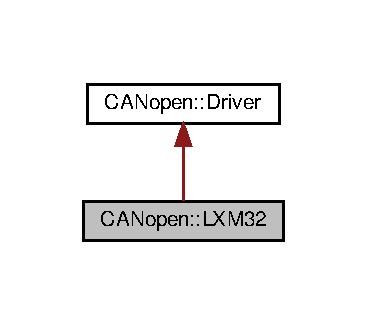
\includegraphics[width=176pt]{class_c_a_nopen_1_1_l_x_m32__inherit__graph}
\end{center}
\end{figure}


Collaboration diagram for C\+A\+Nopen\+:\+:L\+X\+M32\+:\nopagebreak
\begin{figure}[H]
\begin{center}
\leavevmode
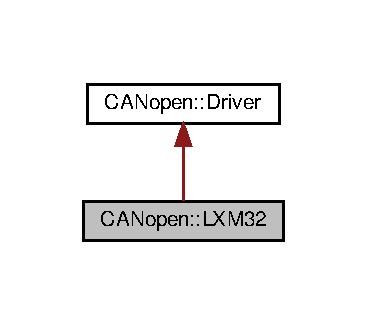
\includegraphics[width=176pt]{class_c_a_nopen_1_1_l_x_m32__coll__graph}
\end{center}
\end{figure}
\subsection*{Public Types}
\begin{DoxyCompactItemize}
\item 
enum \hyperlink{class_c_a_nopen_1_1_l_x_m32_ac925b7d916f09f6b9ede53099ca7f136}{O\+Pmode} \+: uint8\+\_\+t \{ \hyperlink{class_c_a_nopen_1_1_l_x_m32_ac925b7d916f09f6b9ede53099ca7f136a5eb9a2719ae06e38895740e123321dbc}{Profile\+Position} = 1, 
\hyperlink{class_c_a_nopen_1_1_l_x_m32_ac925b7d916f09f6b9ede53099ca7f136a9bcb0eb48795ad942925719d59cdc1c9}{Profile\+Velocity} = 2
 \}
\end{DoxyCompactItemize}
\subsection*{Public Member Functions}
\begin{DoxyCompactItemize}
\item 
\hyperlink{class_c_a_nopen_1_1_l_x_m32_aa4a3e84b72c79b4d47e9f842a8977f98}{L\+X\+M32} (const char $\ast$ifname, uint16\+\_\+t can\+\_\+id, bool verbose=false)
\begin{DoxyCompactList}\small\item\em Constructor. \end{DoxyCompactList}\item 
int32\+\_\+t \hyperlink{class_c_a_nopen_1_1_l_x_m32_a3d325b9b19432dc05240ccfc328363d9}{init} ()
\item 
void \hyperlink{class_c_a_nopen_1_1_l_x_m32_a22ac99e21e6c32626046d320c7bd3605}{get\+\_\+param} ()
\item 
void \hyperlink{class_c_a_nopen_1_1_l_x_m32_a201d8f9da28994a92612e2618b7a1167}{print\+\_\+status} ()
\item 
void \hyperlink{class_c_a_nopen_1_1_l_x_m32_a545b23fab3528a8039bb2cc62808f9f5}{print\+\_\+control} ()
\end{DoxyCompactItemize}


\subsection{Detailed Description}


Definition at line 10 of file C\+A\+Nopen\+\_\+lxm32.\+h.



\subsection{Member Enumeration Documentation}
\mbox{\Hypertarget{class_c_a_nopen_1_1_l_x_m32_ac925b7d916f09f6b9ede53099ca7f136}\label{class_c_a_nopen_1_1_l_x_m32_ac925b7d916f09f6b9ede53099ca7f136}} 
\index{C\+A\+Nopen\+::\+L\+X\+M32@{C\+A\+Nopen\+::\+L\+X\+M32}!O\+Pmode@{O\+Pmode}}
\index{O\+Pmode@{O\+Pmode}!C\+A\+Nopen\+::\+L\+X\+M32@{C\+A\+Nopen\+::\+L\+X\+M32}}
\subsubsection{\texorpdfstring{O\+Pmode}{OPmode}}
{\footnotesize\ttfamily enum \hyperlink{class_c_a_nopen_1_1_l_x_m32_ac925b7d916f09f6b9ede53099ca7f136}{C\+A\+Nopen\+::\+L\+X\+M32\+::\+O\+Pmode} \+: uint8\+\_\+t}

\begin{DoxyEnumFields}{Enumerator}
\raisebox{\heightof{T}}[0pt][0pt]{\index{Profile\+Position@{Profile\+Position}!C\+A\+Nopen\+::\+L\+X\+M32@{C\+A\+Nopen\+::\+L\+X\+M32}}\index{C\+A\+Nopen\+::\+L\+X\+M32@{C\+A\+Nopen\+::\+L\+X\+M32}!Profile\+Position@{Profile\+Position}}}\mbox{\Hypertarget{class_c_a_nopen_1_1_l_x_m32_ac925b7d916f09f6b9ede53099ca7f136a5eb9a2719ae06e38895740e123321dbc}\label{class_c_a_nopen_1_1_l_x_m32_ac925b7d916f09f6b9ede53099ca7f136a5eb9a2719ae06e38895740e123321dbc}} 
Profile\+Position&\\
\hline

\raisebox{\heightof{T}}[0pt][0pt]{\index{Profile\+Velocity@{Profile\+Velocity}!C\+A\+Nopen\+::\+L\+X\+M32@{C\+A\+Nopen\+::\+L\+X\+M32}}\index{C\+A\+Nopen\+::\+L\+X\+M32@{C\+A\+Nopen\+::\+L\+X\+M32}!Profile\+Velocity@{Profile\+Velocity}}}\mbox{\Hypertarget{class_c_a_nopen_1_1_l_x_m32_ac925b7d916f09f6b9ede53099ca7f136a9bcb0eb48795ad942925719d59cdc1c9}\label{class_c_a_nopen_1_1_l_x_m32_ac925b7d916f09f6b9ede53099ca7f136a9bcb0eb48795ad942925719d59cdc1c9}} 
Profile\+Velocity&\\
\hline

\end{DoxyEnumFields}


Definition at line 12 of file C\+A\+Nopen\+\_\+lxm32.\+h.



\subsection{Constructor \& Destructor Documentation}
\mbox{\Hypertarget{class_c_a_nopen_1_1_l_x_m32_aa4a3e84b72c79b4d47e9f842a8977f98}\label{class_c_a_nopen_1_1_l_x_m32_aa4a3e84b72c79b4d47e9f842a8977f98}} 
\index{C\+A\+Nopen\+::\+L\+X\+M32@{C\+A\+Nopen\+::\+L\+X\+M32}!L\+X\+M32@{L\+X\+M32}}
\index{L\+X\+M32@{L\+X\+M32}!C\+A\+Nopen\+::\+L\+X\+M32@{C\+A\+Nopen\+::\+L\+X\+M32}}
\subsubsection{\texorpdfstring{L\+X\+M32()}{LXM32()}}
{\footnotesize\ttfamily L\+X\+M32\+::\+L\+X\+M32 (\begin{DoxyParamCaption}\item[{const char $\ast$}]{ifname,  }\item[{uint16\+\_\+t}]{can\+\_\+id,  }\item[{bool}]{verbose = {\ttfamily false} }\end{DoxyParamCaption})}



Constructor. 


\begin{DoxyParams}{Parameters}
{\em ifname} & \+: Name of the C\+AN interface. \\
\hline
{\em can\+\_\+id} & \+: Node C\+AN ID of the driver. \\
\hline
\end{DoxyParams}


Definition at line 3 of file C\+A\+Nopen\+\_\+lxm32.\+cpp.



\subsection{Member Function Documentation}
\mbox{\Hypertarget{class_c_a_nopen_1_1_l_x_m32_a22ac99e21e6c32626046d320c7bd3605}\label{class_c_a_nopen_1_1_l_x_m32_a22ac99e21e6c32626046d320c7bd3605}} 
\index{C\+A\+Nopen\+::\+L\+X\+M32@{C\+A\+Nopen\+::\+L\+X\+M32}!get\+\_\+param@{get\+\_\+param}}
\index{get\+\_\+param@{get\+\_\+param}!C\+A\+Nopen\+::\+L\+X\+M32@{C\+A\+Nopen\+::\+L\+X\+M32}}
\subsubsection{\texorpdfstring{get\+\_\+param()}{get\_param()}}
{\footnotesize\ttfamily void C\+A\+Nopen\+::\+L\+X\+M32\+::get\+\_\+param (\begin{DoxyParamCaption}{ }\end{DoxyParamCaption})}

\mbox{\Hypertarget{class_c_a_nopen_1_1_l_x_m32_a3d325b9b19432dc05240ccfc328363d9}\label{class_c_a_nopen_1_1_l_x_m32_a3d325b9b19432dc05240ccfc328363d9}} 
\index{C\+A\+Nopen\+::\+L\+X\+M32@{C\+A\+Nopen\+::\+L\+X\+M32}!init@{init}}
\index{init@{init}!C\+A\+Nopen\+::\+L\+X\+M32@{C\+A\+Nopen\+::\+L\+X\+M32}}
\subsubsection{\texorpdfstring{init()}{init()}}
{\footnotesize\ttfamily void L\+X\+M32\+::init (\begin{DoxyParamCaption}{ }\end{DoxyParamCaption})}



Definition at line 14 of file C\+A\+Nopen\+\_\+lxm32.\+cpp.

\mbox{\Hypertarget{class_c_a_nopen_1_1_l_x_m32_a545b23fab3528a8039bb2cc62808f9f5}\label{class_c_a_nopen_1_1_l_x_m32_a545b23fab3528a8039bb2cc62808f9f5}} 
\index{C\+A\+Nopen\+::\+L\+X\+M32@{C\+A\+Nopen\+::\+L\+X\+M32}!print\+\_\+control@{print\+\_\+control}}
\index{print\+\_\+control@{print\+\_\+control}!C\+A\+Nopen\+::\+L\+X\+M32@{C\+A\+Nopen\+::\+L\+X\+M32}}
\subsubsection{\texorpdfstring{print\+\_\+control()}{print\_control()}}
{\footnotesize\ttfamily void L\+X\+M32\+::print\+\_\+control (\begin{DoxyParamCaption}{ }\end{DoxyParamCaption})}



Definition at line 152 of file C\+A\+Nopen\+\_\+lxm32.\+cpp.

\mbox{\Hypertarget{class_c_a_nopen_1_1_l_x_m32_a201d8f9da28994a92612e2618b7a1167}\label{class_c_a_nopen_1_1_l_x_m32_a201d8f9da28994a92612e2618b7a1167}} 
\index{C\+A\+Nopen\+::\+L\+X\+M32@{C\+A\+Nopen\+::\+L\+X\+M32}!print\+\_\+status@{print\+\_\+status}}
\index{print\+\_\+status@{print\+\_\+status}!C\+A\+Nopen\+::\+L\+X\+M32@{C\+A\+Nopen\+::\+L\+X\+M32}}
\subsubsection{\texorpdfstring{print\+\_\+status()}{print\_status()}}
{\footnotesize\ttfamily void L\+X\+M32\+::print\+\_\+status (\begin{DoxyParamCaption}{ }\end{DoxyParamCaption})}



Definition at line 95 of file C\+A\+Nopen\+\_\+lxm32.\+cpp.



The documentation for this class was generated from the following files\+:\begin{DoxyCompactItemize}
\item 
/home/adev/\+Documents/\+S\+T\+E\+C\+H/lxm32/include/\hyperlink{_c_a_nopen__lxm32_8h}{C\+A\+Nopen\+\_\+lxm32.\+h}\item 
/home/adev/\+Documents/\+S\+T\+E\+C\+H/lxm32/src/\hyperlink{_c_a_nopen__lxm32_8cpp}{C\+A\+Nopen\+\_\+lxm32.\+cpp}\end{DoxyCompactItemize}

\hypertarget{class_c_a_nopen_1_1_message}{}\section{C\+A\+Nopen\+:\+:Message Class Reference}
\label{class_c_a_nopen_1_1_message}\index{C\+A\+Nopen\+::\+Message@{C\+A\+Nopen\+::\+Message}}


{\ttfamily \#include $<$message.\+h$>$}



Inheritance diagram for C\+A\+Nopen\+:\+:Message\+:\nopagebreak
\begin{figure}[H]
\begin{center}
\leavevmode
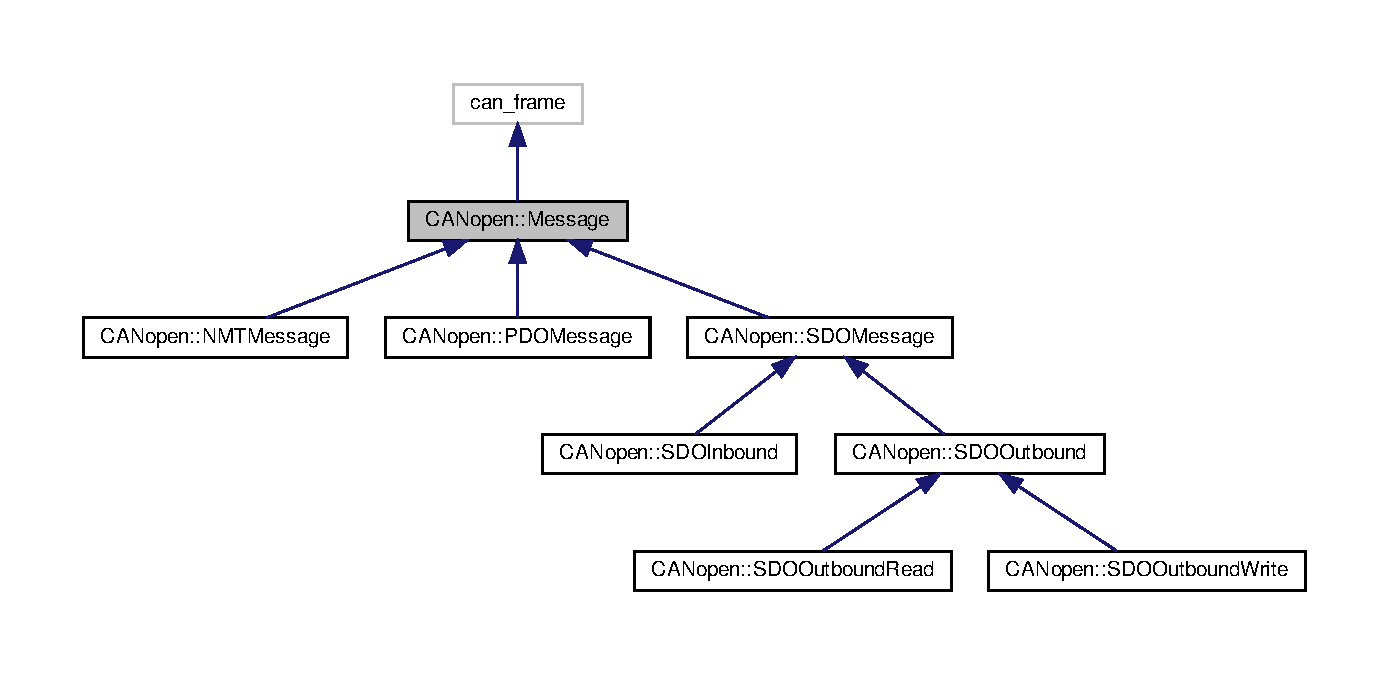
\includegraphics[width=350pt]{class_c_a_nopen_1_1_message__inherit__graph}
\end{center}
\end{figure}


Collaboration diagram for C\+A\+Nopen\+:\+:Message\+:\nopagebreak
\begin{figure}[H]
\begin{center}
\leavevmode
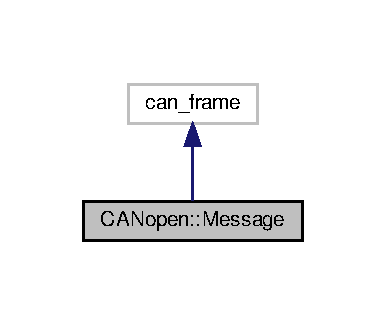
\includegraphics[width=185pt]{class_c_a_nopen_1_1_message__coll__graph}
\end{center}
\end{figure}
\subsection*{Public Types}
\begin{DoxyCompactItemize}
\item 
enum \hyperlink{class_c_a_nopen_1_1_message_a0f8f95e4ea1284011cd122629edc5468}{Function\+Code} \+: uint32\+\_\+t \{ \newline
\hyperlink{class_c_a_nopen_1_1_message_a0f8f95e4ea1284011cd122629edc5468a9772de90d6832671c05553ecc93168ce}{N\+MT} = 0, 
\hyperlink{class_c_a_nopen_1_1_message_a0f8f95e4ea1284011cd122629edc5468acf827d4fddf4af5908ff22d480ec3f9f}{Emergency} = 0x80, 
\hyperlink{class_c_a_nopen_1_1_message_a0f8f95e4ea1284011cd122629edc5468a439fca8488e446232afad47ea72326f4}{Sync} = 0x80, 
\hyperlink{class_c_a_nopen_1_1_message_a0f8f95e4ea1284011cd122629edc5468a4cce8d38cc9a387ac2553c97082934c7}{Time\+Stamp} = 0x100, 
\newline
\hyperlink{class_c_a_nopen_1_1_message_a0f8f95e4ea1284011cd122629edc5468aea8753e3c4fecde547db28a4a01f4fea}{P\+D\+O1\+Transmit} = 0x180, 
\hyperlink{class_c_a_nopen_1_1_message_a0f8f95e4ea1284011cd122629edc5468a289816747eb21454c97a2c0de54bd7bd}{P\+D\+O1\+Receive} = 0x200, 
\hyperlink{class_c_a_nopen_1_1_message_a0f8f95e4ea1284011cd122629edc5468a644cdb60cf2ec10f6f509c6dac09c7e7}{P\+D\+O2\+Transmit} = 0x280, 
\hyperlink{class_c_a_nopen_1_1_message_a0f8f95e4ea1284011cd122629edc5468ae19e8c5160acfaab1c140c21789138e3}{P\+D\+O2\+Receive} = 0x300, 
\newline
\hyperlink{class_c_a_nopen_1_1_message_a0f8f95e4ea1284011cd122629edc5468ac15c2cbe07eac4f1fdc102927deadcdc}{P\+D\+O3\+Transmit} = 0x380, 
\hyperlink{class_c_a_nopen_1_1_message_a0f8f95e4ea1284011cd122629edc5468ab059d1f4ab6ed9bb993e5d37aea6eba1}{P\+D\+O3\+Receive} = 0x400, 
\hyperlink{class_c_a_nopen_1_1_message_a0f8f95e4ea1284011cd122629edc5468a46d53ca55e462afcab565303b212656c}{P\+D\+O4\+Transmit} = 0x480, 
\hyperlink{class_c_a_nopen_1_1_message_a0f8f95e4ea1284011cd122629edc5468a45f4fc29142533ab1395bd971c12be9b}{P\+D\+O4\+Receive} = 0x500, 
\newline
\hyperlink{class_c_a_nopen_1_1_message_a0f8f95e4ea1284011cd122629edc5468ab54b9a53105e0549e5fc07ef1ee6b91a}{S\+D\+O\+Transmit} = 0x580, 
\hyperlink{class_c_a_nopen_1_1_message_a0f8f95e4ea1284011cd122629edc5468a720fb5202eef37017f7f58ac195c5949}{S\+D\+O\+Receive} = 0x600, 
\hyperlink{class_c_a_nopen_1_1_message_a0f8f95e4ea1284011cd122629edc5468aea5e380d61d7dbbbb5f4655e3fbdc65c}{Heartbeat} = 0x700
 \}
\end{DoxyCompactItemize}
\subsection*{Public Member Functions}
\begin{DoxyCompactItemize}
\item 
\hyperlink{class_c_a_nopen_1_1_message_a90dac1b216099b2a29f7b4deb3ccced8}{Message} ()=default
\item 
\hyperlink{class_c_a_nopen_1_1_message_a77a8c09ad0711fa4b574a8b88d983441}{Message} (const can\+\_\+frame \&other)
\item 
\hyperlink{class_c_a_nopen_1_1_message_ace3b5218ab769fb1e642b82b2d3fc7d3}{Message} (uint32\+\_\+t cob\+\_\+id, \hyperlink{class_c_a_nopen_1_1_payload}{Payload} \hyperlink{class_c_a_nopen_1_1_message_a65be4f77771803bed521cbbf2316271b}{payload})
\item 
\hyperlink{class_c_a_nopen_1_1_message_a0f8f95e4ea1284011cd122629edc5468}{Function\+Code} \hyperlink{class_c_a_nopen_1_1_message_a83d9901bbd77dcca9b44d68fd1e604b8}{function\+\_\+code} ()
\item 
uint8\+\_\+t \hyperlink{class_c_a_nopen_1_1_message_a845fe0c7682bd6eeef0a5dd87b5e3c63}{node\+\_\+id} ()
\item 
\hyperlink{class_c_a_nopen_1_1_payload}{Payload} \hyperlink{class_c_a_nopen_1_1_message_a65be4f77771803bed521cbbf2316271b}{payload} ()
\item 
std\+::string \hyperlink{class_c_a_nopen_1_1_message_a0d3aade9268f612f1918d64e8c6057b7}{to\+\_\+string} ()
\end{DoxyCompactItemize}


\subsection{Detailed Description}


Definition at line 10 of file message.\+h.



\subsection{Member Enumeration Documentation}
\mbox{\Hypertarget{class_c_a_nopen_1_1_message_a0f8f95e4ea1284011cd122629edc5468}\label{class_c_a_nopen_1_1_message_a0f8f95e4ea1284011cd122629edc5468}} 
\index{C\+A\+Nopen\+::\+Message@{C\+A\+Nopen\+::\+Message}!Function\+Code@{Function\+Code}}
\index{Function\+Code@{Function\+Code}!C\+A\+Nopen\+::\+Message@{C\+A\+Nopen\+::\+Message}}
\subsubsection{\texorpdfstring{Function\+Code}{FunctionCode}}
{\footnotesize\ttfamily enum \hyperlink{class_c_a_nopen_1_1_message_a0f8f95e4ea1284011cd122629edc5468}{C\+A\+Nopen\+::\+Message\+::\+Function\+Code} \+: uint32\+\_\+t}

\begin{DoxyEnumFields}{Enumerator}
\raisebox{\heightof{T}}[0pt][0pt]{\index{N\+MT@{N\+MT}!C\+A\+Nopen\+::\+Message@{C\+A\+Nopen\+::\+Message}}\index{C\+A\+Nopen\+::\+Message@{C\+A\+Nopen\+::\+Message}!N\+MT@{N\+MT}}}\mbox{\Hypertarget{class_c_a_nopen_1_1_message_a0f8f95e4ea1284011cd122629edc5468a9772de90d6832671c05553ecc93168ce}\label{class_c_a_nopen_1_1_message_a0f8f95e4ea1284011cd122629edc5468a9772de90d6832671c05553ecc93168ce}} 
N\+MT&\\
\hline

\raisebox{\heightof{T}}[0pt][0pt]{\index{Emergency@{Emergency}!C\+A\+Nopen\+::\+Message@{C\+A\+Nopen\+::\+Message}}\index{C\+A\+Nopen\+::\+Message@{C\+A\+Nopen\+::\+Message}!Emergency@{Emergency}}}\mbox{\Hypertarget{class_c_a_nopen_1_1_message_a0f8f95e4ea1284011cd122629edc5468acf827d4fddf4af5908ff22d480ec3f9f}\label{class_c_a_nopen_1_1_message_a0f8f95e4ea1284011cd122629edc5468acf827d4fddf4af5908ff22d480ec3f9f}} 
Emergency&\\
\hline

\raisebox{\heightof{T}}[0pt][0pt]{\index{Sync@{Sync}!C\+A\+Nopen\+::\+Message@{C\+A\+Nopen\+::\+Message}}\index{C\+A\+Nopen\+::\+Message@{C\+A\+Nopen\+::\+Message}!Sync@{Sync}}}\mbox{\Hypertarget{class_c_a_nopen_1_1_message_a0f8f95e4ea1284011cd122629edc5468a439fca8488e446232afad47ea72326f4}\label{class_c_a_nopen_1_1_message_a0f8f95e4ea1284011cd122629edc5468a439fca8488e446232afad47ea72326f4}} 
Sync&\\
\hline

\raisebox{\heightof{T}}[0pt][0pt]{\index{Time\+Stamp@{Time\+Stamp}!C\+A\+Nopen\+::\+Message@{C\+A\+Nopen\+::\+Message}}\index{C\+A\+Nopen\+::\+Message@{C\+A\+Nopen\+::\+Message}!Time\+Stamp@{Time\+Stamp}}}\mbox{\Hypertarget{class_c_a_nopen_1_1_message_a0f8f95e4ea1284011cd122629edc5468a4cce8d38cc9a387ac2553c97082934c7}\label{class_c_a_nopen_1_1_message_a0f8f95e4ea1284011cd122629edc5468a4cce8d38cc9a387ac2553c97082934c7}} 
Time\+Stamp&\\
\hline

\raisebox{\heightof{T}}[0pt][0pt]{\index{P\+D\+O1\+Transmit@{P\+D\+O1\+Transmit}!C\+A\+Nopen\+::\+Message@{C\+A\+Nopen\+::\+Message}}\index{C\+A\+Nopen\+::\+Message@{C\+A\+Nopen\+::\+Message}!P\+D\+O1\+Transmit@{P\+D\+O1\+Transmit}}}\mbox{\Hypertarget{class_c_a_nopen_1_1_message_a0f8f95e4ea1284011cd122629edc5468aea8753e3c4fecde547db28a4a01f4fea}\label{class_c_a_nopen_1_1_message_a0f8f95e4ea1284011cd122629edc5468aea8753e3c4fecde547db28a4a01f4fea}} 
P\+D\+O1\+Transmit&\\
\hline

\raisebox{\heightof{T}}[0pt][0pt]{\index{P\+D\+O1\+Receive@{P\+D\+O1\+Receive}!C\+A\+Nopen\+::\+Message@{C\+A\+Nopen\+::\+Message}}\index{C\+A\+Nopen\+::\+Message@{C\+A\+Nopen\+::\+Message}!P\+D\+O1\+Receive@{P\+D\+O1\+Receive}}}\mbox{\Hypertarget{class_c_a_nopen_1_1_message_a0f8f95e4ea1284011cd122629edc5468a289816747eb21454c97a2c0de54bd7bd}\label{class_c_a_nopen_1_1_message_a0f8f95e4ea1284011cd122629edc5468a289816747eb21454c97a2c0de54bd7bd}} 
P\+D\+O1\+Receive&\\
\hline

\raisebox{\heightof{T}}[0pt][0pt]{\index{P\+D\+O2\+Transmit@{P\+D\+O2\+Transmit}!C\+A\+Nopen\+::\+Message@{C\+A\+Nopen\+::\+Message}}\index{C\+A\+Nopen\+::\+Message@{C\+A\+Nopen\+::\+Message}!P\+D\+O2\+Transmit@{P\+D\+O2\+Transmit}}}\mbox{\Hypertarget{class_c_a_nopen_1_1_message_a0f8f95e4ea1284011cd122629edc5468a644cdb60cf2ec10f6f509c6dac09c7e7}\label{class_c_a_nopen_1_1_message_a0f8f95e4ea1284011cd122629edc5468a644cdb60cf2ec10f6f509c6dac09c7e7}} 
P\+D\+O2\+Transmit&\\
\hline

\raisebox{\heightof{T}}[0pt][0pt]{\index{P\+D\+O2\+Receive@{P\+D\+O2\+Receive}!C\+A\+Nopen\+::\+Message@{C\+A\+Nopen\+::\+Message}}\index{C\+A\+Nopen\+::\+Message@{C\+A\+Nopen\+::\+Message}!P\+D\+O2\+Receive@{P\+D\+O2\+Receive}}}\mbox{\Hypertarget{class_c_a_nopen_1_1_message_a0f8f95e4ea1284011cd122629edc5468ae19e8c5160acfaab1c140c21789138e3}\label{class_c_a_nopen_1_1_message_a0f8f95e4ea1284011cd122629edc5468ae19e8c5160acfaab1c140c21789138e3}} 
P\+D\+O2\+Receive&\\
\hline

\raisebox{\heightof{T}}[0pt][0pt]{\index{P\+D\+O3\+Transmit@{P\+D\+O3\+Transmit}!C\+A\+Nopen\+::\+Message@{C\+A\+Nopen\+::\+Message}}\index{C\+A\+Nopen\+::\+Message@{C\+A\+Nopen\+::\+Message}!P\+D\+O3\+Transmit@{P\+D\+O3\+Transmit}}}\mbox{\Hypertarget{class_c_a_nopen_1_1_message_a0f8f95e4ea1284011cd122629edc5468ac15c2cbe07eac4f1fdc102927deadcdc}\label{class_c_a_nopen_1_1_message_a0f8f95e4ea1284011cd122629edc5468ac15c2cbe07eac4f1fdc102927deadcdc}} 
P\+D\+O3\+Transmit&\\
\hline

\raisebox{\heightof{T}}[0pt][0pt]{\index{P\+D\+O3\+Receive@{P\+D\+O3\+Receive}!C\+A\+Nopen\+::\+Message@{C\+A\+Nopen\+::\+Message}}\index{C\+A\+Nopen\+::\+Message@{C\+A\+Nopen\+::\+Message}!P\+D\+O3\+Receive@{P\+D\+O3\+Receive}}}\mbox{\Hypertarget{class_c_a_nopen_1_1_message_a0f8f95e4ea1284011cd122629edc5468ab059d1f4ab6ed9bb993e5d37aea6eba1}\label{class_c_a_nopen_1_1_message_a0f8f95e4ea1284011cd122629edc5468ab059d1f4ab6ed9bb993e5d37aea6eba1}} 
P\+D\+O3\+Receive&\\
\hline

\raisebox{\heightof{T}}[0pt][0pt]{\index{P\+D\+O4\+Transmit@{P\+D\+O4\+Transmit}!C\+A\+Nopen\+::\+Message@{C\+A\+Nopen\+::\+Message}}\index{C\+A\+Nopen\+::\+Message@{C\+A\+Nopen\+::\+Message}!P\+D\+O4\+Transmit@{P\+D\+O4\+Transmit}}}\mbox{\Hypertarget{class_c_a_nopen_1_1_message_a0f8f95e4ea1284011cd122629edc5468a46d53ca55e462afcab565303b212656c}\label{class_c_a_nopen_1_1_message_a0f8f95e4ea1284011cd122629edc5468a46d53ca55e462afcab565303b212656c}} 
P\+D\+O4\+Transmit&\\
\hline

\raisebox{\heightof{T}}[0pt][0pt]{\index{P\+D\+O4\+Receive@{P\+D\+O4\+Receive}!C\+A\+Nopen\+::\+Message@{C\+A\+Nopen\+::\+Message}}\index{C\+A\+Nopen\+::\+Message@{C\+A\+Nopen\+::\+Message}!P\+D\+O4\+Receive@{P\+D\+O4\+Receive}}}\mbox{\Hypertarget{class_c_a_nopen_1_1_message_a0f8f95e4ea1284011cd122629edc5468a45f4fc29142533ab1395bd971c12be9b}\label{class_c_a_nopen_1_1_message_a0f8f95e4ea1284011cd122629edc5468a45f4fc29142533ab1395bd971c12be9b}} 
P\+D\+O4\+Receive&\\
\hline

\raisebox{\heightof{T}}[0pt][0pt]{\index{S\+D\+O\+Transmit@{S\+D\+O\+Transmit}!C\+A\+Nopen\+::\+Message@{C\+A\+Nopen\+::\+Message}}\index{C\+A\+Nopen\+::\+Message@{C\+A\+Nopen\+::\+Message}!S\+D\+O\+Transmit@{S\+D\+O\+Transmit}}}\mbox{\Hypertarget{class_c_a_nopen_1_1_message_a0f8f95e4ea1284011cd122629edc5468ab54b9a53105e0549e5fc07ef1ee6b91a}\label{class_c_a_nopen_1_1_message_a0f8f95e4ea1284011cd122629edc5468ab54b9a53105e0549e5fc07ef1ee6b91a}} 
S\+D\+O\+Transmit&\\
\hline

\raisebox{\heightof{T}}[0pt][0pt]{\index{S\+D\+O\+Receive@{S\+D\+O\+Receive}!C\+A\+Nopen\+::\+Message@{C\+A\+Nopen\+::\+Message}}\index{C\+A\+Nopen\+::\+Message@{C\+A\+Nopen\+::\+Message}!S\+D\+O\+Receive@{S\+D\+O\+Receive}}}\mbox{\Hypertarget{class_c_a_nopen_1_1_message_a0f8f95e4ea1284011cd122629edc5468a720fb5202eef37017f7f58ac195c5949}\label{class_c_a_nopen_1_1_message_a0f8f95e4ea1284011cd122629edc5468a720fb5202eef37017f7f58ac195c5949}} 
S\+D\+O\+Receive&\\
\hline

\raisebox{\heightof{T}}[0pt][0pt]{\index{Heartbeat@{Heartbeat}!C\+A\+Nopen\+::\+Message@{C\+A\+Nopen\+::\+Message}}\index{C\+A\+Nopen\+::\+Message@{C\+A\+Nopen\+::\+Message}!Heartbeat@{Heartbeat}}}\mbox{\Hypertarget{class_c_a_nopen_1_1_message_a0f8f95e4ea1284011cd122629edc5468aea5e380d61d7dbbbb5f4655e3fbdc65c}\label{class_c_a_nopen_1_1_message_a0f8f95e4ea1284011cd122629edc5468aea5e380d61d7dbbbb5f4655e3fbdc65c}} 
Heartbeat&\\
\hline

\end{DoxyEnumFields}


Definition at line 12 of file message.\+h.



\subsection{Constructor \& Destructor Documentation}
\mbox{\Hypertarget{class_c_a_nopen_1_1_message_a90dac1b216099b2a29f7b4deb3ccced8}\label{class_c_a_nopen_1_1_message_a90dac1b216099b2a29f7b4deb3ccced8}} 
\index{C\+A\+Nopen\+::\+Message@{C\+A\+Nopen\+::\+Message}!Message@{Message}}
\index{Message@{Message}!C\+A\+Nopen\+::\+Message@{C\+A\+Nopen\+::\+Message}}
\subsubsection{\texorpdfstring{Message()}{Message()}\hspace{0.1cm}{\footnotesize\ttfamily [1/3]}}
{\footnotesize\ttfamily C\+A\+Nopen\+::\+Message\+::\+Message (\begin{DoxyParamCaption}{ }\end{DoxyParamCaption})\hspace{0.3cm}{\ttfamily [default]}}

\mbox{\Hypertarget{class_c_a_nopen_1_1_message_a77a8c09ad0711fa4b574a8b88d983441}\label{class_c_a_nopen_1_1_message_a77a8c09ad0711fa4b574a8b88d983441}} 
\index{C\+A\+Nopen\+::\+Message@{C\+A\+Nopen\+::\+Message}!Message@{Message}}
\index{Message@{Message}!C\+A\+Nopen\+::\+Message@{C\+A\+Nopen\+::\+Message}}
\subsubsection{\texorpdfstring{Message()}{Message()}\hspace{0.1cm}{\footnotesize\ttfamily [2/3]}}
{\footnotesize\ttfamily C\+A\+Nopen\+::\+Message\+::\+Message (\begin{DoxyParamCaption}\item[{const can\+\_\+frame \&}]{other }\end{DoxyParamCaption})}



Definition at line 13 of file message.\+cpp.

\mbox{\Hypertarget{class_c_a_nopen_1_1_message_ace3b5218ab769fb1e642b82b2d3fc7d3}\label{class_c_a_nopen_1_1_message_ace3b5218ab769fb1e642b82b2d3fc7d3}} 
\index{C\+A\+Nopen\+::\+Message@{C\+A\+Nopen\+::\+Message}!Message@{Message}}
\index{Message@{Message}!C\+A\+Nopen\+::\+Message@{C\+A\+Nopen\+::\+Message}}
\subsubsection{\texorpdfstring{Message()}{Message()}\hspace{0.1cm}{\footnotesize\ttfamily [3/3]}}
{\footnotesize\ttfamily C\+A\+Nopen\+::\+Message\+::\+Message (\begin{DoxyParamCaption}\item[{uint32\+\_\+t}]{cob\+\_\+id,  }\item[{\hyperlink{class_c_a_nopen_1_1_payload}{Payload}}]{payload }\end{DoxyParamCaption})}



Definition at line 6 of file message.\+cpp.



\subsection{Member Function Documentation}
\mbox{\Hypertarget{class_c_a_nopen_1_1_message_a83d9901bbd77dcca9b44d68fd1e604b8}\label{class_c_a_nopen_1_1_message_a83d9901bbd77dcca9b44d68fd1e604b8}} 
\index{C\+A\+Nopen\+::\+Message@{C\+A\+Nopen\+::\+Message}!function\+\_\+code@{function\+\_\+code}}
\index{function\+\_\+code@{function\+\_\+code}!C\+A\+Nopen\+::\+Message@{C\+A\+Nopen\+::\+Message}}
\subsubsection{\texorpdfstring{function\+\_\+code()}{function\_code()}}
{\footnotesize\ttfamily \hyperlink{class_c_a_nopen_1_1_message_a0f8f95e4ea1284011cd122629edc5468}{Message\+::\+Function\+Code} C\+A\+Nopen\+::\+Message\+::function\+\_\+code (\begin{DoxyParamCaption}{ }\end{DoxyParamCaption})}



Definition at line 18 of file message.\+cpp.

\mbox{\Hypertarget{class_c_a_nopen_1_1_message_a845fe0c7682bd6eeef0a5dd87b5e3c63}\label{class_c_a_nopen_1_1_message_a845fe0c7682bd6eeef0a5dd87b5e3c63}} 
\index{C\+A\+Nopen\+::\+Message@{C\+A\+Nopen\+::\+Message}!node\+\_\+id@{node\+\_\+id}}
\index{node\+\_\+id@{node\+\_\+id}!C\+A\+Nopen\+::\+Message@{C\+A\+Nopen\+::\+Message}}
\subsubsection{\texorpdfstring{node\+\_\+id()}{node\_id()}}
{\footnotesize\ttfamily uint8\+\_\+t C\+A\+Nopen\+::\+Message\+::node\+\_\+id (\begin{DoxyParamCaption}{ }\end{DoxyParamCaption})}



Definition at line 23 of file message.\+cpp.

\mbox{\Hypertarget{class_c_a_nopen_1_1_message_a65be4f77771803bed521cbbf2316271b}\label{class_c_a_nopen_1_1_message_a65be4f77771803bed521cbbf2316271b}} 
\index{C\+A\+Nopen\+::\+Message@{C\+A\+Nopen\+::\+Message}!payload@{payload}}
\index{payload@{payload}!C\+A\+Nopen\+::\+Message@{C\+A\+Nopen\+::\+Message}}
\subsubsection{\texorpdfstring{payload()}{payload()}}
{\footnotesize\ttfamily \hyperlink{class_c_a_nopen_1_1_payload}{Payload} C\+A\+Nopen\+::\+Message\+::payload (\begin{DoxyParamCaption}{ }\end{DoxyParamCaption})}



Definition at line 28 of file message.\+cpp.

\mbox{\Hypertarget{class_c_a_nopen_1_1_message_a0d3aade9268f612f1918d64e8c6057b7}\label{class_c_a_nopen_1_1_message_a0d3aade9268f612f1918d64e8c6057b7}} 
\index{C\+A\+Nopen\+::\+Message@{C\+A\+Nopen\+::\+Message}!to\+\_\+string@{to\+\_\+string}}
\index{to\+\_\+string@{to\+\_\+string}!C\+A\+Nopen\+::\+Message@{C\+A\+Nopen\+::\+Message}}
\subsubsection{\texorpdfstring{to\+\_\+string()}{to\_string()}}
{\footnotesize\ttfamily std\+::string C\+A\+Nopen\+::\+Message\+::to\+\_\+string (\begin{DoxyParamCaption}{ }\end{DoxyParamCaption})}



Definition at line 33 of file message.\+cpp.



The documentation for this class was generated from the following files\+:\begin{DoxyCompactItemize}
\item 
/home/adev/\+Documents/\+S\+T\+E\+C\+H/lxm32/lib/canopen/include/\hyperlink{message_8h}{message.\+h}\item 
/home/adev/\+Documents/\+S\+T\+E\+C\+H/lxm32/lib/canopen/src/\hyperlink{message_8cpp}{message.\+cpp}\end{DoxyCompactItemize}

\hypertarget{class_c_a_nopen_1_1_n_m_t_message}{}\section{C\+A\+Nopen\+:\+:N\+M\+T\+Message Class Reference}
\label{class_c_a_nopen_1_1_n_m_t_message}\index{C\+A\+Nopen\+::\+N\+M\+T\+Message@{C\+A\+Nopen\+::\+N\+M\+T\+Message}}


{\ttfamily \#include $<$nmt.\+h$>$}



Inheritance diagram for C\+A\+Nopen\+:\+:N\+M\+T\+Message\+:\nopagebreak
\begin{figure}[H]
\begin{center}
\leavevmode
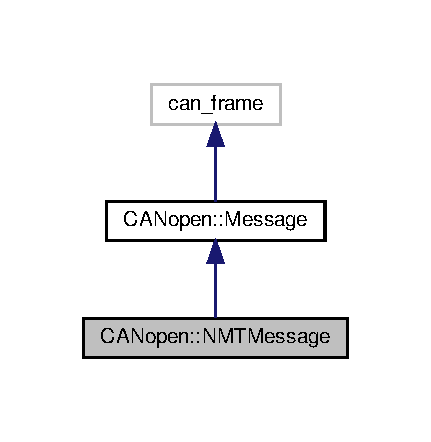
\includegraphics[width=207pt]{class_c_a_nopen_1_1_n_m_t_message__inherit__graph}
\end{center}
\end{figure}


Collaboration diagram for C\+A\+Nopen\+:\+:N\+M\+T\+Message\+:\nopagebreak
\begin{figure}[H]
\begin{center}
\leavevmode
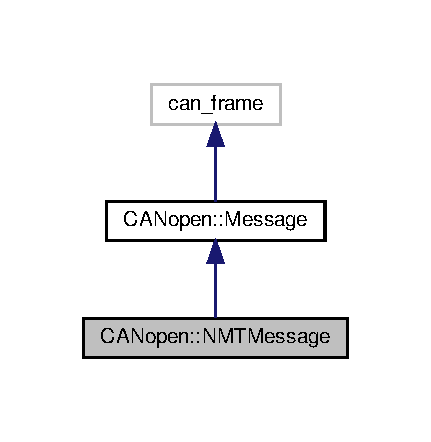
\includegraphics[width=207pt]{class_c_a_nopen_1_1_n_m_t_message__coll__graph}
\end{center}
\end{figure}
\subsection*{Public Types}
\begin{DoxyCompactItemize}
\item 
enum \hyperlink{class_c_a_nopen_1_1_n_m_t_message_a20257f9fc32b84adc9196fd436f15e95}{Code} \+: uint8\+\_\+t \{ \newline
\hyperlink{class_c_a_nopen_1_1_n_m_t_message_a20257f9fc32b84adc9196fd436f15e95a7fe77fc2c4080c22ffe1833947ccbe9a}{Initialising} = 0, 
\hyperlink{class_c_a_nopen_1_1_n_m_t_message_a20257f9fc32b84adc9196fd436f15e95a545e9a577466163fb58669287c3c6b41}{Go\+To\+Operational} = 0x01, 
\hyperlink{class_c_a_nopen_1_1_n_m_t_message_a20257f9fc32b84adc9196fd436f15e95a7809df81e01fe09e4419db0473038d43}{Go\+To\+Stopped} = 0x02, 
\hyperlink{class_c_a_nopen_1_1_n_m_t_message_a20257f9fc32b84adc9196fd436f15e95a7d6f2ebee6ed9eb78ce062f2c39fcb3f}{Stopped} = 0x04, 
\newline
\hyperlink{class_c_a_nopen_1_1_n_m_t_message_a20257f9fc32b84adc9196fd436f15e95a8060d997fd31646e2abe3ecef93e5224}{Operational} = 0x05, 
\hyperlink{class_c_a_nopen_1_1_n_m_t_message_a20257f9fc32b84adc9196fd436f15e95af0059e344b7e07bdcb934da702a529ad}{Pre\+Operational} = 0x7f, 
\hyperlink{class_c_a_nopen_1_1_n_m_t_message_a20257f9fc32b84adc9196fd436f15e95aac9ea51398ac876f28caa68e5060dc49}{Go\+To\+Pre\+Operational} = 0x80, 
\hyperlink{class_c_a_nopen_1_1_n_m_t_message_a20257f9fc32b84adc9196fd436f15e95a8f2baac414d139872bfef60ecea4ebd8}{Go\+To\+Reset\+Node} = 0x81, 
\newline
\hyperlink{class_c_a_nopen_1_1_n_m_t_message_a20257f9fc32b84adc9196fd436f15e95adc2beca1ff30670ddbe1181b6ba82a0f}{Go\+To\+Reset\+Communication} = 0x82
 \}
\end{DoxyCompactItemize}
\subsection*{Public Member Functions}
\begin{DoxyCompactItemize}
\item 
\hyperlink{class_c_a_nopen_1_1_n_m_t_message_a5e38ad7cb1464480121e527589f4d18f}{N\+M\+T\+Message} ()=default
\item 
\hyperlink{class_c_a_nopen_1_1_n_m_t_message_ae691342a23d0bffa2a98861099c19fcc}{N\+M\+T\+Message} (const can\+\_\+frame \&other)
\item 
\hyperlink{class_c_a_nopen_1_1_n_m_t_message_a5939adf6f14706495b9e734f8412f5d4}{N\+M\+T\+Message} (\hyperlink{class_c_a_nopen_1_1_n_m_t_message_a20257f9fc32b84adc9196fd436f15e95}{Code} code, uint8\+\_\+t \hyperlink{class_c_a_nopen_1_1_message_a845fe0c7682bd6eeef0a5dd87b5e3c63}{node\+\_\+id})
\end{DoxyCompactItemize}


\subsection{Detailed Description}


Definition at line 7 of file nmt.\+h.



\subsection{Member Enumeration Documentation}
\mbox{\Hypertarget{class_c_a_nopen_1_1_n_m_t_message_a20257f9fc32b84adc9196fd436f15e95}\label{class_c_a_nopen_1_1_n_m_t_message_a20257f9fc32b84adc9196fd436f15e95}} 
\index{C\+A\+Nopen\+::\+N\+M\+T\+Message@{C\+A\+Nopen\+::\+N\+M\+T\+Message}!Code@{Code}}
\index{Code@{Code}!C\+A\+Nopen\+::\+N\+M\+T\+Message@{C\+A\+Nopen\+::\+N\+M\+T\+Message}}
\subsubsection{\texorpdfstring{Code}{Code}}
{\footnotesize\ttfamily enum \hyperlink{class_c_a_nopen_1_1_n_m_t_message_a20257f9fc32b84adc9196fd436f15e95}{C\+A\+Nopen\+::\+N\+M\+T\+Message\+::\+Code} \+: uint8\+\_\+t}

\begin{DoxyEnumFields}{Enumerator}
\raisebox{\heightof{T}}[0pt][0pt]{\index{Initialising@{Initialising}!C\+A\+Nopen\+::\+N\+M\+T\+Message@{C\+A\+Nopen\+::\+N\+M\+T\+Message}}\index{C\+A\+Nopen\+::\+N\+M\+T\+Message@{C\+A\+Nopen\+::\+N\+M\+T\+Message}!Initialising@{Initialising}}}\mbox{\Hypertarget{class_c_a_nopen_1_1_n_m_t_message_a20257f9fc32b84adc9196fd436f15e95a7fe77fc2c4080c22ffe1833947ccbe9a}\label{class_c_a_nopen_1_1_n_m_t_message_a20257f9fc32b84adc9196fd436f15e95a7fe77fc2c4080c22ffe1833947ccbe9a}} 
Initialising&\\
\hline

\raisebox{\heightof{T}}[0pt][0pt]{\index{Go\+To\+Operational@{Go\+To\+Operational}!C\+A\+Nopen\+::\+N\+M\+T\+Message@{C\+A\+Nopen\+::\+N\+M\+T\+Message}}\index{C\+A\+Nopen\+::\+N\+M\+T\+Message@{C\+A\+Nopen\+::\+N\+M\+T\+Message}!Go\+To\+Operational@{Go\+To\+Operational}}}\mbox{\Hypertarget{class_c_a_nopen_1_1_n_m_t_message_a20257f9fc32b84adc9196fd436f15e95a545e9a577466163fb58669287c3c6b41}\label{class_c_a_nopen_1_1_n_m_t_message_a20257f9fc32b84adc9196fd436f15e95a545e9a577466163fb58669287c3c6b41}} 
Go\+To\+Operational&\\
\hline

\raisebox{\heightof{T}}[0pt][0pt]{\index{Go\+To\+Stopped@{Go\+To\+Stopped}!C\+A\+Nopen\+::\+N\+M\+T\+Message@{C\+A\+Nopen\+::\+N\+M\+T\+Message}}\index{C\+A\+Nopen\+::\+N\+M\+T\+Message@{C\+A\+Nopen\+::\+N\+M\+T\+Message}!Go\+To\+Stopped@{Go\+To\+Stopped}}}\mbox{\Hypertarget{class_c_a_nopen_1_1_n_m_t_message_a20257f9fc32b84adc9196fd436f15e95a7809df81e01fe09e4419db0473038d43}\label{class_c_a_nopen_1_1_n_m_t_message_a20257f9fc32b84adc9196fd436f15e95a7809df81e01fe09e4419db0473038d43}} 
Go\+To\+Stopped&\\
\hline

\raisebox{\heightof{T}}[0pt][0pt]{\index{Stopped@{Stopped}!C\+A\+Nopen\+::\+N\+M\+T\+Message@{C\+A\+Nopen\+::\+N\+M\+T\+Message}}\index{C\+A\+Nopen\+::\+N\+M\+T\+Message@{C\+A\+Nopen\+::\+N\+M\+T\+Message}!Stopped@{Stopped}}}\mbox{\Hypertarget{class_c_a_nopen_1_1_n_m_t_message_a20257f9fc32b84adc9196fd436f15e95a7d6f2ebee6ed9eb78ce062f2c39fcb3f}\label{class_c_a_nopen_1_1_n_m_t_message_a20257f9fc32b84adc9196fd436f15e95a7d6f2ebee6ed9eb78ce062f2c39fcb3f}} 
Stopped&\\
\hline

\raisebox{\heightof{T}}[0pt][0pt]{\index{Operational@{Operational}!C\+A\+Nopen\+::\+N\+M\+T\+Message@{C\+A\+Nopen\+::\+N\+M\+T\+Message}}\index{C\+A\+Nopen\+::\+N\+M\+T\+Message@{C\+A\+Nopen\+::\+N\+M\+T\+Message}!Operational@{Operational}}}\mbox{\Hypertarget{class_c_a_nopen_1_1_n_m_t_message_a20257f9fc32b84adc9196fd436f15e95a8060d997fd31646e2abe3ecef93e5224}\label{class_c_a_nopen_1_1_n_m_t_message_a20257f9fc32b84adc9196fd436f15e95a8060d997fd31646e2abe3ecef93e5224}} 
Operational&\\
\hline

\raisebox{\heightof{T}}[0pt][0pt]{\index{Pre\+Operational@{Pre\+Operational}!C\+A\+Nopen\+::\+N\+M\+T\+Message@{C\+A\+Nopen\+::\+N\+M\+T\+Message}}\index{C\+A\+Nopen\+::\+N\+M\+T\+Message@{C\+A\+Nopen\+::\+N\+M\+T\+Message}!Pre\+Operational@{Pre\+Operational}}}\mbox{\Hypertarget{class_c_a_nopen_1_1_n_m_t_message_a20257f9fc32b84adc9196fd436f15e95af0059e344b7e07bdcb934da702a529ad}\label{class_c_a_nopen_1_1_n_m_t_message_a20257f9fc32b84adc9196fd436f15e95af0059e344b7e07bdcb934da702a529ad}} 
Pre\+Operational&\\
\hline

\raisebox{\heightof{T}}[0pt][0pt]{\index{Go\+To\+Pre\+Operational@{Go\+To\+Pre\+Operational}!C\+A\+Nopen\+::\+N\+M\+T\+Message@{C\+A\+Nopen\+::\+N\+M\+T\+Message}}\index{C\+A\+Nopen\+::\+N\+M\+T\+Message@{C\+A\+Nopen\+::\+N\+M\+T\+Message}!Go\+To\+Pre\+Operational@{Go\+To\+Pre\+Operational}}}\mbox{\Hypertarget{class_c_a_nopen_1_1_n_m_t_message_a20257f9fc32b84adc9196fd436f15e95aac9ea51398ac876f28caa68e5060dc49}\label{class_c_a_nopen_1_1_n_m_t_message_a20257f9fc32b84adc9196fd436f15e95aac9ea51398ac876f28caa68e5060dc49}} 
Go\+To\+Pre\+Operational&\\
\hline

\raisebox{\heightof{T}}[0pt][0pt]{\index{Go\+To\+Reset\+Node@{Go\+To\+Reset\+Node}!C\+A\+Nopen\+::\+N\+M\+T\+Message@{C\+A\+Nopen\+::\+N\+M\+T\+Message}}\index{C\+A\+Nopen\+::\+N\+M\+T\+Message@{C\+A\+Nopen\+::\+N\+M\+T\+Message}!Go\+To\+Reset\+Node@{Go\+To\+Reset\+Node}}}\mbox{\Hypertarget{class_c_a_nopen_1_1_n_m_t_message_a20257f9fc32b84adc9196fd436f15e95a8f2baac414d139872bfef60ecea4ebd8}\label{class_c_a_nopen_1_1_n_m_t_message_a20257f9fc32b84adc9196fd436f15e95a8f2baac414d139872bfef60ecea4ebd8}} 
Go\+To\+Reset\+Node&\\
\hline

\raisebox{\heightof{T}}[0pt][0pt]{\index{Go\+To\+Reset\+Communication@{Go\+To\+Reset\+Communication}!C\+A\+Nopen\+::\+N\+M\+T\+Message@{C\+A\+Nopen\+::\+N\+M\+T\+Message}}\index{C\+A\+Nopen\+::\+N\+M\+T\+Message@{C\+A\+Nopen\+::\+N\+M\+T\+Message}!Go\+To\+Reset\+Communication@{Go\+To\+Reset\+Communication}}}\mbox{\Hypertarget{class_c_a_nopen_1_1_n_m_t_message_a20257f9fc32b84adc9196fd436f15e95adc2beca1ff30670ddbe1181b6ba82a0f}\label{class_c_a_nopen_1_1_n_m_t_message_a20257f9fc32b84adc9196fd436f15e95adc2beca1ff30670ddbe1181b6ba82a0f}} 
Go\+To\+Reset\+Communication&\\
\hline

\end{DoxyEnumFields}


Definition at line 10 of file nmt.\+h.



\subsection{Constructor \& Destructor Documentation}
\mbox{\Hypertarget{class_c_a_nopen_1_1_n_m_t_message_a5e38ad7cb1464480121e527589f4d18f}\label{class_c_a_nopen_1_1_n_m_t_message_a5e38ad7cb1464480121e527589f4d18f}} 
\index{C\+A\+Nopen\+::\+N\+M\+T\+Message@{C\+A\+Nopen\+::\+N\+M\+T\+Message}!N\+M\+T\+Message@{N\+M\+T\+Message}}
\index{N\+M\+T\+Message@{N\+M\+T\+Message}!C\+A\+Nopen\+::\+N\+M\+T\+Message@{C\+A\+Nopen\+::\+N\+M\+T\+Message}}
\subsubsection{\texorpdfstring{N\+M\+T\+Message()}{NMTMessage()}\hspace{0.1cm}{\footnotesize\ttfamily [1/3]}}
{\footnotesize\ttfamily C\+A\+Nopen\+::\+N\+M\+T\+Message\+::\+N\+M\+T\+Message (\begin{DoxyParamCaption}{ }\end{DoxyParamCaption})\hspace{0.3cm}{\ttfamily [default]}}

\mbox{\Hypertarget{class_c_a_nopen_1_1_n_m_t_message_ae691342a23d0bffa2a98861099c19fcc}\label{class_c_a_nopen_1_1_n_m_t_message_ae691342a23d0bffa2a98861099c19fcc}} 
\index{C\+A\+Nopen\+::\+N\+M\+T\+Message@{C\+A\+Nopen\+::\+N\+M\+T\+Message}!N\+M\+T\+Message@{N\+M\+T\+Message}}
\index{N\+M\+T\+Message@{N\+M\+T\+Message}!C\+A\+Nopen\+::\+N\+M\+T\+Message@{C\+A\+Nopen\+::\+N\+M\+T\+Message}}
\subsubsection{\texorpdfstring{N\+M\+T\+Message()}{NMTMessage()}\hspace{0.1cm}{\footnotesize\ttfamily [2/3]}}
{\footnotesize\ttfamily C\+A\+Nopen\+::\+N\+M\+T\+Message\+::\+N\+M\+T\+Message (\begin{DoxyParamCaption}\item[{const can\+\_\+frame \&}]{other }\end{DoxyParamCaption})}



Definition at line 4 of file nmt.\+cpp.

\mbox{\Hypertarget{class_c_a_nopen_1_1_n_m_t_message_a5939adf6f14706495b9e734f8412f5d4}\label{class_c_a_nopen_1_1_n_m_t_message_a5939adf6f14706495b9e734f8412f5d4}} 
\index{C\+A\+Nopen\+::\+N\+M\+T\+Message@{C\+A\+Nopen\+::\+N\+M\+T\+Message}!N\+M\+T\+Message@{N\+M\+T\+Message}}
\index{N\+M\+T\+Message@{N\+M\+T\+Message}!C\+A\+Nopen\+::\+N\+M\+T\+Message@{C\+A\+Nopen\+::\+N\+M\+T\+Message}}
\subsubsection{\texorpdfstring{N\+M\+T\+Message()}{NMTMessage()}\hspace{0.1cm}{\footnotesize\ttfamily [3/3]}}
{\footnotesize\ttfamily C\+A\+Nopen\+::\+N\+M\+T\+Message\+::\+N\+M\+T\+Message (\begin{DoxyParamCaption}\item[{\hyperlink{class_c_a_nopen_1_1_n_m_t_message_a20257f9fc32b84adc9196fd436f15e95}{Code}}]{code,  }\item[{uint8\+\_\+t}]{node\+\_\+id }\end{DoxyParamCaption})}



Definition at line 9 of file nmt.\+cpp.



The documentation for this class was generated from the following files\+:\begin{DoxyCompactItemize}
\item 
/home/adev/\+Documents/\+S\+T\+E\+C\+H/lxm32/lib/canopen/include/\hyperlink{nmt_8h}{nmt.\+h}\item 
/home/adev/\+Documents/\+S\+T\+E\+C\+H/lxm32/lib/canopen/src/\hyperlink{nmt_8cpp}{nmt.\+cpp}\end{DoxyCompactItemize}

\hypertarget{class_c_a_nopen_1_1_payload}{}\section{C\+A\+Nopen\+:\+:Payload Class Reference}
\label{class_c_a_nopen_1_1_payload}\index{C\+A\+Nopen\+::\+Payload@{C\+A\+Nopen\+::\+Payload}}


{\ttfamily \#include $<$payload.\+h$>$}



Inheritance diagram for C\+A\+Nopen\+:\+:Payload\+:\nopagebreak
\begin{figure}[H]
\begin{center}
\leavevmode
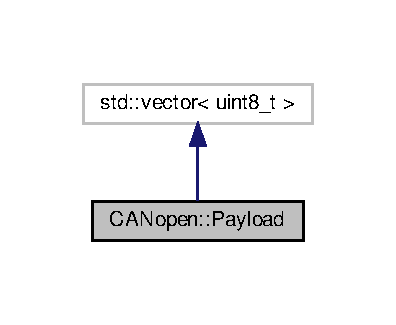
\includegraphics[width=190pt]{class_c_a_nopen_1_1_payload__inherit__graph}
\end{center}
\end{figure}


Collaboration diagram for C\+A\+Nopen\+:\+:Payload\+:\nopagebreak
\begin{figure}[H]
\begin{center}
\leavevmode
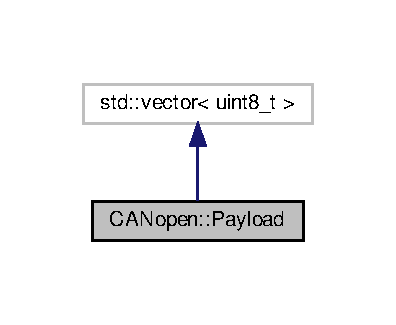
\includegraphics[width=190pt]{class_c_a_nopen_1_1_payload__coll__graph}
\end{center}
\end{figure}
\subsection*{Public Member Functions}
\begin{DoxyCompactItemize}
\item 
\hyperlink{class_c_a_nopen_1_1_payload_a1b22524210c44e52820944fdd041484f}{Payload} ()=default
\item 
\hyperlink{class_c_a_nopen_1_1_payload_a1177f8bbace9e9779c7549ae7ace1681}{Payload} (const \hyperlink{class_c_a_nopen_1_1_payload}{Payload} \&)=default
\item 
\hyperlink{class_c_a_nopen_1_1_payload_ab0769e01554cc879840463e2a55eab0e}{Payload} (const std\+::vector$<$ uint8\+\_\+t $>$ \&other)
\item 
{\footnotesize template$<$typename T $>$ }\\\hyperlink{class_c_a_nopen_1_1_payload_a769f01631bd710d3b37f07cc2753b889}{Payload} (T \hyperlink{class_c_a_nopen_1_1_payload_aef05ef8cfc8b9ba4170891f3168a726b}{value})
\item 
\hyperlink{class_c_a_nopen_1_1_payload}{Payload} \& \hyperlink{class_c_a_nopen_1_1_payload_a646541a9ec787a3fcdbbcba153e8553c}{operator=} (const \hyperlink{class_c_a_nopen_1_1_payload}{Payload} \&)=default
\item 
{\footnotesize template$<$typename T $>$ }\\T \& \hyperlink{class_c_a_nopen_1_1_payload_aef05ef8cfc8b9ba4170891f3168a726b}{value} (unsigned begin=0)
\item 
{\footnotesize template$<$typename T $>$ }\\\hyperlink{class_c_a_nopen_1_1_payload}{Payload} \& \hyperlink{class_c_a_nopen_1_1_payload_a7386499320878a2ab437f419f9970d7c}{operator$<$$<$} (T \&\hyperlink{class_c_a_nopen_1_1_payload_aef05ef8cfc8b9ba4170891f3168a726b}{value})
\item 
\hyperlink{class_c_a_nopen_1_1_payload_a61e7092a555d000dfd59c6942823c9f1}{operator std\+::string} () const
\end{DoxyCompactItemize}
\subsection*{Static Public Member Functions}
\begin{DoxyCompactItemize}
\item 
{\footnotesize template$<$typename T $>$ }\\static \hyperlink{class_c_a_nopen_1_1_payload}{Payload} \hyperlink{class_c_a_nopen_1_1_payload_a1264ea3795f5d7e1a1a153121b15e25f}{from\+\_\+data} (const T \&\hyperlink{class_c_a_nopen_1_1_payload_aef05ef8cfc8b9ba4170891f3168a726b}{value})
\item 
{\footnotesize template$<$typename T1 , typename... Ts$>$ }\\static \hyperlink{class_c_a_nopen_1_1_payload}{Payload} \hyperlink{class_c_a_nopen_1_1_payload_aeb95d2ae0204e12a46df4d7c97788739}{from\+\_\+data} (const T1 \&\hyperlink{class_c_a_nopen_1_1_payload_aef05ef8cfc8b9ba4170891f3168a726b}{value}, const Ts \&\&... others)
\end{DoxyCompactItemize}


\subsection{Detailed Description}


Definition at line 11 of file payload.\+h.



\subsection{Constructor \& Destructor Documentation}
\mbox{\Hypertarget{class_c_a_nopen_1_1_payload_a1b22524210c44e52820944fdd041484f}\label{class_c_a_nopen_1_1_payload_a1b22524210c44e52820944fdd041484f}} 
\index{C\+A\+Nopen\+::\+Payload@{C\+A\+Nopen\+::\+Payload}!Payload@{Payload}}
\index{Payload@{Payload}!C\+A\+Nopen\+::\+Payload@{C\+A\+Nopen\+::\+Payload}}
\subsubsection{\texorpdfstring{Payload()}{Payload()}\hspace{0.1cm}{\footnotesize\ttfamily [1/4]}}
{\footnotesize\ttfamily C\+A\+Nopen\+::\+Payload\+::\+Payload (\begin{DoxyParamCaption}{ }\end{DoxyParamCaption})\hspace{0.3cm}{\ttfamily [default]}}

\mbox{\Hypertarget{class_c_a_nopen_1_1_payload_a1177f8bbace9e9779c7549ae7ace1681}\label{class_c_a_nopen_1_1_payload_a1177f8bbace9e9779c7549ae7ace1681}} 
\index{C\+A\+Nopen\+::\+Payload@{C\+A\+Nopen\+::\+Payload}!Payload@{Payload}}
\index{Payload@{Payload}!C\+A\+Nopen\+::\+Payload@{C\+A\+Nopen\+::\+Payload}}
\subsubsection{\texorpdfstring{Payload()}{Payload()}\hspace{0.1cm}{\footnotesize\ttfamily [2/4]}}
{\footnotesize\ttfamily C\+A\+Nopen\+::\+Payload\+::\+Payload (\begin{DoxyParamCaption}\item[{const \hyperlink{class_c_a_nopen_1_1_payload}{Payload} \&}]{ }\end{DoxyParamCaption})\hspace{0.3cm}{\ttfamily [default]}}

\mbox{\Hypertarget{class_c_a_nopen_1_1_payload_ab0769e01554cc879840463e2a55eab0e}\label{class_c_a_nopen_1_1_payload_ab0769e01554cc879840463e2a55eab0e}} 
\index{C\+A\+Nopen\+::\+Payload@{C\+A\+Nopen\+::\+Payload}!Payload@{Payload}}
\index{Payload@{Payload}!C\+A\+Nopen\+::\+Payload@{C\+A\+Nopen\+::\+Payload}}
\subsubsection{\texorpdfstring{Payload()}{Payload()}\hspace{0.1cm}{\footnotesize\ttfamily [3/4]}}
{\footnotesize\ttfamily C\+A\+Nopen\+::\+Payload\+::\+Payload (\begin{DoxyParamCaption}\item[{const std\+::vector$<$ uint8\+\_\+t $>$ \&}]{other }\end{DoxyParamCaption})}



Definition at line 6 of file payload.\+cpp.

\mbox{\Hypertarget{class_c_a_nopen_1_1_payload_a769f01631bd710d3b37f07cc2753b889}\label{class_c_a_nopen_1_1_payload_a769f01631bd710d3b37f07cc2753b889}} 
\index{C\+A\+Nopen\+::\+Payload@{C\+A\+Nopen\+::\+Payload}!Payload@{Payload}}
\index{Payload@{Payload}!C\+A\+Nopen\+::\+Payload@{C\+A\+Nopen\+::\+Payload}}
\subsubsection{\texorpdfstring{Payload()}{Payload()}\hspace{0.1cm}{\footnotesize\ttfamily [4/4]}}
{\footnotesize\ttfamily template$<$typename T $>$ \\
C\+A\+Nopen\+::\+Payload\+::\+Payload (\begin{DoxyParamCaption}\item[{T}]{value }\end{DoxyParamCaption})\hspace{0.3cm}{\ttfamily [inline]}}



Definition at line 18 of file payload.\+h.



\subsection{Member Function Documentation}
\mbox{\Hypertarget{class_c_a_nopen_1_1_payload_a1264ea3795f5d7e1a1a153121b15e25f}\label{class_c_a_nopen_1_1_payload_a1264ea3795f5d7e1a1a153121b15e25f}} 
\index{C\+A\+Nopen\+::\+Payload@{C\+A\+Nopen\+::\+Payload}!from\+\_\+data@{from\+\_\+data}}
\index{from\+\_\+data@{from\+\_\+data}!C\+A\+Nopen\+::\+Payload@{C\+A\+Nopen\+::\+Payload}}
\subsubsection{\texorpdfstring{from\+\_\+data()}{from\_data()}\hspace{0.1cm}{\footnotesize\ttfamily [1/2]}}
{\footnotesize\ttfamily template$<$typename T $>$ \\
static \hyperlink{class_c_a_nopen_1_1_payload}{Payload} C\+A\+Nopen\+::\+Payload\+::from\+\_\+data (\begin{DoxyParamCaption}\item[{const T \&}]{value }\end{DoxyParamCaption})\hspace{0.3cm}{\ttfamily [inline]}, {\ttfamily [static]}}



Definition at line 28 of file payload.\+h.

\mbox{\Hypertarget{class_c_a_nopen_1_1_payload_aeb95d2ae0204e12a46df4d7c97788739}\label{class_c_a_nopen_1_1_payload_aeb95d2ae0204e12a46df4d7c97788739}} 
\index{C\+A\+Nopen\+::\+Payload@{C\+A\+Nopen\+::\+Payload}!from\+\_\+data@{from\+\_\+data}}
\index{from\+\_\+data@{from\+\_\+data}!C\+A\+Nopen\+::\+Payload@{C\+A\+Nopen\+::\+Payload}}
\subsubsection{\texorpdfstring{from\+\_\+data()}{from\_data()}\hspace{0.1cm}{\footnotesize\ttfamily [2/2]}}
{\footnotesize\ttfamily template$<$typename T1 , typename... Ts$>$ \\
static \hyperlink{class_c_a_nopen_1_1_payload}{Payload} C\+A\+Nopen\+::\+Payload\+::from\+\_\+data (\begin{DoxyParamCaption}\item[{const T1 \&}]{value,  }\item[{const Ts \&\&...}]{others }\end{DoxyParamCaption})\hspace{0.3cm}{\ttfamily [inline]}, {\ttfamily [static]}}



Definition at line 38 of file payload.\+h.

\mbox{\Hypertarget{class_c_a_nopen_1_1_payload_a61e7092a555d000dfd59c6942823c9f1}\label{class_c_a_nopen_1_1_payload_a61e7092a555d000dfd59c6942823c9f1}} 
\index{C\+A\+Nopen\+::\+Payload@{C\+A\+Nopen\+::\+Payload}!operator std\+::string@{operator std\+::string}}
\index{operator std\+::string@{operator std\+::string}!C\+A\+Nopen\+::\+Payload@{C\+A\+Nopen\+::\+Payload}}
\subsubsection{\texorpdfstring{operator std\+::string()}{operator std::string()}}
{\footnotesize\ttfamily C\+A\+Nopen\+::\+Payload\+::operator std\+::string (\begin{DoxyParamCaption}{ }\end{DoxyParamCaption}) const}



Definition at line 11 of file payload.\+cpp.

\mbox{\Hypertarget{class_c_a_nopen_1_1_payload_a7386499320878a2ab437f419f9970d7c}\label{class_c_a_nopen_1_1_payload_a7386499320878a2ab437f419f9970d7c}} 
\index{C\+A\+Nopen\+::\+Payload@{C\+A\+Nopen\+::\+Payload}!operator$<$$<$@{operator$<$$<$}}
\index{operator$<$$<$@{operator$<$$<$}!C\+A\+Nopen\+::\+Payload@{C\+A\+Nopen\+::\+Payload}}
\subsubsection{\texorpdfstring{operator$<$$<$()}{operator<<()}}
{\footnotesize\ttfamily template$<$typename T $>$ \\
\hyperlink{class_c_a_nopen_1_1_payload}{Payload}\& C\+A\+Nopen\+::\+Payload\+::operator$<$$<$ (\begin{DoxyParamCaption}\item[{T \&}]{value }\end{DoxyParamCaption})\hspace{0.3cm}{\ttfamily [inline]}}



Definition at line 50 of file payload.\+h.

\mbox{\Hypertarget{class_c_a_nopen_1_1_payload_a646541a9ec787a3fcdbbcba153e8553c}\label{class_c_a_nopen_1_1_payload_a646541a9ec787a3fcdbbcba153e8553c}} 
\index{C\+A\+Nopen\+::\+Payload@{C\+A\+Nopen\+::\+Payload}!operator=@{operator=}}
\index{operator=@{operator=}!C\+A\+Nopen\+::\+Payload@{C\+A\+Nopen\+::\+Payload}}
\subsubsection{\texorpdfstring{operator=()}{operator=()}}
{\footnotesize\ttfamily \hyperlink{class_c_a_nopen_1_1_payload}{Payload}\& C\+A\+Nopen\+::\+Payload\+::operator= (\begin{DoxyParamCaption}\item[{const \hyperlink{class_c_a_nopen_1_1_payload}{Payload} \&}]{ }\end{DoxyParamCaption})\hspace{0.3cm}{\ttfamily [default]}}

\mbox{\Hypertarget{class_c_a_nopen_1_1_payload_aef05ef8cfc8b9ba4170891f3168a726b}\label{class_c_a_nopen_1_1_payload_aef05ef8cfc8b9ba4170891f3168a726b}} 
\index{C\+A\+Nopen\+::\+Payload@{C\+A\+Nopen\+::\+Payload}!value@{value}}
\index{value@{value}!C\+A\+Nopen\+::\+Payload@{C\+A\+Nopen\+::\+Payload}}
\subsubsection{\texorpdfstring{value()}{value()}}
{\footnotesize\ttfamily template$<$typename T $>$ \\
T\& C\+A\+Nopen\+::\+Payload\+::value (\begin{DoxyParamCaption}\item[{unsigned}]{begin = {\ttfamily 0} }\end{DoxyParamCaption})\hspace{0.3cm}{\ttfamily [inline]}}



Definition at line 44 of file payload.\+h.



The documentation for this class was generated from the following files\+:\begin{DoxyCompactItemize}
\item 
/home/adev/\+Documents/\+S\+T\+E\+C\+H/lxm32/lib/canopen/include/\hyperlink{payload_8h}{payload.\+h}\item 
/home/adev/\+Documents/\+S\+T\+E\+C\+H/lxm32/lib/canopen/src/\hyperlink{payload_8cpp}{payload.\+cpp}\end{DoxyCompactItemize}

\hypertarget{class_c_a_nopen_1_1_p_d_o_message}{}\section{C\+A\+Nopen\+:\+:P\+D\+O\+Message Class Reference}
\label{class_c_a_nopen_1_1_p_d_o_message}\index{C\+A\+Nopen\+::\+P\+D\+O\+Message@{C\+A\+Nopen\+::\+P\+D\+O\+Message}}


{\ttfamily \#include $<$pdo.\+h$>$}



Inheritance diagram for C\+A\+Nopen\+:\+:P\+D\+O\+Message\+:\nopagebreak
\begin{figure}[H]
\begin{center}
\leavevmode
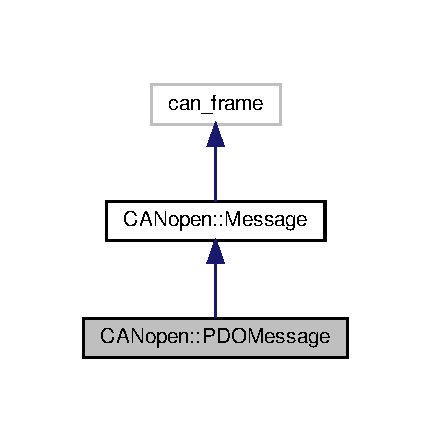
\includegraphics[width=207pt]{class_c_a_nopen_1_1_p_d_o_message__inherit__graph}
\end{center}
\end{figure}


Collaboration diagram for C\+A\+Nopen\+:\+:P\+D\+O\+Message\+:\nopagebreak
\begin{figure}[H]
\begin{center}
\leavevmode
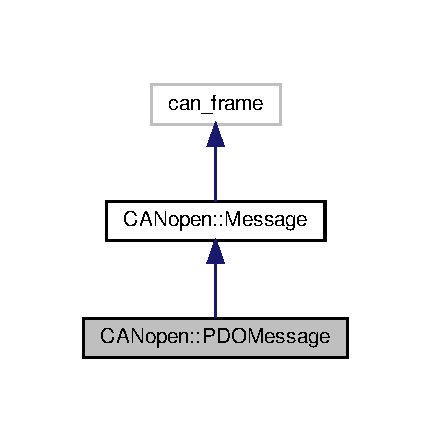
\includegraphics[width=207pt]{class_c_a_nopen_1_1_p_d_o_message__coll__graph}
\end{center}
\end{figure}
\subsection*{Public Types}
\begin{DoxyCompactItemize}
\item 
enum \hyperlink{class_c_a_nopen_1_1_p_d_o_message_ab46579ce08cec30d0bc60428053cb39f}{P\+D\+O\+Function\+Code} \+: uint32\+\_\+t \{ \newline
\hyperlink{class_c_a_nopen_1_1_p_d_o_message_ab46579ce08cec30d0bc60428053cb39fabfcc66bfc93e03a72bb931e5bd636798}{P\+D\+O1\+Transmit} = Message\+:\+:P\+D\+O1\+Transmit, 
\hyperlink{class_c_a_nopen_1_1_p_d_o_message_ab46579ce08cec30d0bc60428053cb39fa01d2d22755748fca5086b2e4bf6b009e}{P\+D\+O1\+Receive} = Message\+:\+:P\+D\+O1\+Receive, 
\hyperlink{class_c_a_nopen_1_1_p_d_o_message_ab46579ce08cec30d0bc60428053cb39fa13229b4458d1949639c4e635cda6689c}{P\+D\+O2\+Transmit} = Message\+:\+:P\+D\+O2\+Transmit, 
\hyperlink{class_c_a_nopen_1_1_p_d_o_message_ab46579ce08cec30d0bc60428053cb39fa2e653900b8cea5673b6c829c0d40b0f2}{P\+D\+O2\+Receive} = Message\+:\+:P\+D\+O2\+Receive, 
\newline
\hyperlink{class_c_a_nopen_1_1_p_d_o_message_ab46579ce08cec30d0bc60428053cb39fa508480956655988cac3696b73e542753}{P\+D\+O3\+Transmit} = Message\+:\+:P\+D\+O3\+Transmit, 
\hyperlink{class_c_a_nopen_1_1_p_d_o_message_ab46579ce08cec30d0bc60428053cb39fa54205762ad0ee3cae8ff88519454fd2b}{P\+D\+O3\+Receive} = Message\+:\+:P\+D\+O3\+Receive, 
\hyperlink{class_c_a_nopen_1_1_p_d_o_message_ab46579ce08cec30d0bc60428053cb39fa67325f4e5dfd2ce6a2214a73997ac09d}{P\+D\+O4\+Transmit} = Message\+:\+:P\+D\+O4\+Transmit, 
\hyperlink{class_c_a_nopen_1_1_p_d_o_message_ab46579ce08cec30d0bc60428053cb39fa73eba51ebd0e854b545554bf9c92091b}{P\+D\+O4\+Receive} = Message\+:\+:P\+D\+O4\+Receive
 \}
\end{DoxyCompactItemize}
\subsection*{Public Member Functions}
\begin{DoxyCompactItemize}
\item 
\hyperlink{class_c_a_nopen_1_1_p_d_o_message_a9a38d99b2d049eccc56efb307f3619e6}{P\+D\+O\+Message} ()=default
\item 
\hyperlink{class_c_a_nopen_1_1_p_d_o_message_a461a62c471761504043dfcb13f9ec685}{P\+D\+O\+Message} (const can\+\_\+frame \&other)
\item 
\hyperlink{class_c_a_nopen_1_1_p_d_o_message_ae7f8db2be338aaa9cc61f08520fa0c85}{P\+D\+O\+Message} (\hyperlink{class_c_a_nopen_1_1_p_d_o_message_ab46579ce08cec30d0bc60428053cb39f}{P\+D\+O\+Function\+Code} fn, uint8\+\_\+t \hyperlink{class_c_a_nopen_1_1_message_a845fe0c7682bd6eeef0a5dd87b5e3c63}{node\+\_\+id}, \hyperlink{class_c_a_nopen_1_1_payload}{Payload} \hyperlink{class_c_a_nopen_1_1_message_a65be4f77771803bed521cbbf2316271b}{payload})
\end{DoxyCompactItemize}


\subsection{Detailed Description}


Definition at line 8 of file pdo.\+h.



\subsection{Member Enumeration Documentation}
\mbox{\Hypertarget{class_c_a_nopen_1_1_p_d_o_message_ab46579ce08cec30d0bc60428053cb39f}\label{class_c_a_nopen_1_1_p_d_o_message_ab46579ce08cec30d0bc60428053cb39f}} 
\index{C\+A\+Nopen\+::\+P\+D\+O\+Message@{C\+A\+Nopen\+::\+P\+D\+O\+Message}!P\+D\+O\+Function\+Code@{P\+D\+O\+Function\+Code}}
\index{P\+D\+O\+Function\+Code@{P\+D\+O\+Function\+Code}!C\+A\+Nopen\+::\+P\+D\+O\+Message@{C\+A\+Nopen\+::\+P\+D\+O\+Message}}
\subsubsection{\texorpdfstring{P\+D\+O\+Function\+Code}{PDOFunctionCode}}
{\footnotesize\ttfamily enum \hyperlink{class_c_a_nopen_1_1_p_d_o_message_ab46579ce08cec30d0bc60428053cb39f}{C\+A\+Nopen\+::\+P\+D\+O\+Message\+::\+P\+D\+O\+Function\+Code} \+: uint32\+\_\+t}

\begin{DoxyEnumFields}{Enumerator}
\raisebox{\heightof{T}}[0pt][0pt]{\index{P\+D\+O1\+Transmit@{P\+D\+O1\+Transmit}!C\+A\+Nopen\+::\+P\+D\+O\+Message@{C\+A\+Nopen\+::\+P\+D\+O\+Message}}\index{C\+A\+Nopen\+::\+P\+D\+O\+Message@{C\+A\+Nopen\+::\+P\+D\+O\+Message}!P\+D\+O1\+Transmit@{P\+D\+O1\+Transmit}}}\mbox{\Hypertarget{class_c_a_nopen_1_1_p_d_o_message_ab46579ce08cec30d0bc60428053cb39fabfcc66bfc93e03a72bb931e5bd636798}\label{class_c_a_nopen_1_1_p_d_o_message_ab46579ce08cec30d0bc60428053cb39fabfcc66bfc93e03a72bb931e5bd636798}} 
P\+D\+O1\+Transmit&\\
\hline

\raisebox{\heightof{T}}[0pt][0pt]{\index{P\+D\+O1\+Receive@{P\+D\+O1\+Receive}!C\+A\+Nopen\+::\+P\+D\+O\+Message@{C\+A\+Nopen\+::\+P\+D\+O\+Message}}\index{C\+A\+Nopen\+::\+P\+D\+O\+Message@{C\+A\+Nopen\+::\+P\+D\+O\+Message}!P\+D\+O1\+Receive@{P\+D\+O1\+Receive}}}\mbox{\Hypertarget{class_c_a_nopen_1_1_p_d_o_message_ab46579ce08cec30d0bc60428053cb39fa01d2d22755748fca5086b2e4bf6b009e}\label{class_c_a_nopen_1_1_p_d_o_message_ab46579ce08cec30d0bc60428053cb39fa01d2d22755748fca5086b2e4bf6b009e}} 
P\+D\+O1\+Receive&\\
\hline

\raisebox{\heightof{T}}[0pt][0pt]{\index{P\+D\+O2\+Transmit@{P\+D\+O2\+Transmit}!C\+A\+Nopen\+::\+P\+D\+O\+Message@{C\+A\+Nopen\+::\+P\+D\+O\+Message}}\index{C\+A\+Nopen\+::\+P\+D\+O\+Message@{C\+A\+Nopen\+::\+P\+D\+O\+Message}!P\+D\+O2\+Transmit@{P\+D\+O2\+Transmit}}}\mbox{\Hypertarget{class_c_a_nopen_1_1_p_d_o_message_ab46579ce08cec30d0bc60428053cb39fa13229b4458d1949639c4e635cda6689c}\label{class_c_a_nopen_1_1_p_d_o_message_ab46579ce08cec30d0bc60428053cb39fa13229b4458d1949639c4e635cda6689c}} 
P\+D\+O2\+Transmit&\\
\hline

\raisebox{\heightof{T}}[0pt][0pt]{\index{P\+D\+O2\+Receive@{P\+D\+O2\+Receive}!C\+A\+Nopen\+::\+P\+D\+O\+Message@{C\+A\+Nopen\+::\+P\+D\+O\+Message}}\index{C\+A\+Nopen\+::\+P\+D\+O\+Message@{C\+A\+Nopen\+::\+P\+D\+O\+Message}!P\+D\+O2\+Receive@{P\+D\+O2\+Receive}}}\mbox{\Hypertarget{class_c_a_nopen_1_1_p_d_o_message_ab46579ce08cec30d0bc60428053cb39fa2e653900b8cea5673b6c829c0d40b0f2}\label{class_c_a_nopen_1_1_p_d_o_message_ab46579ce08cec30d0bc60428053cb39fa2e653900b8cea5673b6c829c0d40b0f2}} 
P\+D\+O2\+Receive&\\
\hline

\raisebox{\heightof{T}}[0pt][0pt]{\index{P\+D\+O3\+Transmit@{P\+D\+O3\+Transmit}!C\+A\+Nopen\+::\+P\+D\+O\+Message@{C\+A\+Nopen\+::\+P\+D\+O\+Message}}\index{C\+A\+Nopen\+::\+P\+D\+O\+Message@{C\+A\+Nopen\+::\+P\+D\+O\+Message}!P\+D\+O3\+Transmit@{P\+D\+O3\+Transmit}}}\mbox{\Hypertarget{class_c_a_nopen_1_1_p_d_o_message_ab46579ce08cec30d0bc60428053cb39fa508480956655988cac3696b73e542753}\label{class_c_a_nopen_1_1_p_d_o_message_ab46579ce08cec30d0bc60428053cb39fa508480956655988cac3696b73e542753}} 
P\+D\+O3\+Transmit&\\
\hline

\raisebox{\heightof{T}}[0pt][0pt]{\index{P\+D\+O3\+Receive@{P\+D\+O3\+Receive}!C\+A\+Nopen\+::\+P\+D\+O\+Message@{C\+A\+Nopen\+::\+P\+D\+O\+Message}}\index{C\+A\+Nopen\+::\+P\+D\+O\+Message@{C\+A\+Nopen\+::\+P\+D\+O\+Message}!P\+D\+O3\+Receive@{P\+D\+O3\+Receive}}}\mbox{\Hypertarget{class_c_a_nopen_1_1_p_d_o_message_ab46579ce08cec30d0bc60428053cb39fa54205762ad0ee3cae8ff88519454fd2b}\label{class_c_a_nopen_1_1_p_d_o_message_ab46579ce08cec30d0bc60428053cb39fa54205762ad0ee3cae8ff88519454fd2b}} 
P\+D\+O3\+Receive&\\
\hline

\raisebox{\heightof{T}}[0pt][0pt]{\index{P\+D\+O4\+Transmit@{P\+D\+O4\+Transmit}!C\+A\+Nopen\+::\+P\+D\+O\+Message@{C\+A\+Nopen\+::\+P\+D\+O\+Message}}\index{C\+A\+Nopen\+::\+P\+D\+O\+Message@{C\+A\+Nopen\+::\+P\+D\+O\+Message}!P\+D\+O4\+Transmit@{P\+D\+O4\+Transmit}}}\mbox{\Hypertarget{class_c_a_nopen_1_1_p_d_o_message_ab46579ce08cec30d0bc60428053cb39fa67325f4e5dfd2ce6a2214a73997ac09d}\label{class_c_a_nopen_1_1_p_d_o_message_ab46579ce08cec30d0bc60428053cb39fa67325f4e5dfd2ce6a2214a73997ac09d}} 
P\+D\+O4\+Transmit&\\
\hline

\raisebox{\heightof{T}}[0pt][0pt]{\index{P\+D\+O4\+Receive@{P\+D\+O4\+Receive}!C\+A\+Nopen\+::\+P\+D\+O\+Message@{C\+A\+Nopen\+::\+P\+D\+O\+Message}}\index{C\+A\+Nopen\+::\+P\+D\+O\+Message@{C\+A\+Nopen\+::\+P\+D\+O\+Message}!P\+D\+O4\+Receive@{P\+D\+O4\+Receive}}}\mbox{\Hypertarget{class_c_a_nopen_1_1_p_d_o_message_ab46579ce08cec30d0bc60428053cb39fa73eba51ebd0e854b545554bf9c92091b}\label{class_c_a_nopen_1_1_p_d_o_message_ab46579ce08cec30d0bc60428053cb39fa73eba51ebd0e854b545554bf9c92091b}} 
P\+D\+O4\+Receive&\\
\hline

\end{DoxyEnumFields}


Definition at line 10 of file pdo.\+h.



\subsection{Constructor \& Destructor Documentation}
\mbox{\Hypertarget{class_c_a_nopen_1_1_p_d_o_message_a9a38d99b2d049eccc56efb307f3619e6}\label{class_c_a_nopen_1_1_p_d_o_message_a9a38d99b2d049eccc56efb307f3619e6}} 
\index{C\+A\+Nopen\+::\+P\+D\+O\+Message@{C\+A\+Nopen\+::\+P\+D\+O\+Message}!P\+D\+O\+Message@{P\+D\+O\+Message}}
\index{P\+D\+O\+Message@{P\+D\+O\+Message}!C\+A\+Nopen\+::\+P\+D\+O\+Message@{C\+A\+Nopen\+::\+P\+D\+O\+Message}}
\subsubsection{\texorpdfstring{P\+D\+O\+Message()}{PDOMessage()}\hspace{0.1cm}{\footnotesize\ttfamily [1/3]}}
{\footnotesize\ttfamily C\+A\+Nopen\+::\+P\+D\+O\+Message\+::\+P\+D\+O\+Message (\begin{DoxyParamCaption}{ }\end{DoxyParamCaption})\hspace{0.3cm}{\ttfamily [default]}}

\mbox{\Hypertarget{class_c_a_nopen_1_1_p_d_o_message_a461a62c471761504043dfcb13f9ec685}\label{class_c_a_nopen_1_1_p_d_o_message_a461a62c471761504043dfcb13f9ec685}} 
\index{C\+A\+Nopen\+::\+P\+D\+O\+Message@{C\+A\+Nopen\+::\+P\+D\+O\+Message}!P\+D\+O\+Message@{P\+D\+O\+Message}}
\index{P\+D\+O\+Message@{P\+D\+O\+Message}!C\+A\+Nopen\+::\+P\+D\+O\+Message@{C\+A\+Nopen\+::\+P\+D\+O\+Message}}
\subsubsection{\texorpdfstring{P\+D\+O\+Message()}{PDOMessage()}\hspace{0.1cm}{\footnotesize\ttfamily [2/3]}}
{\footnotesize\ttfamily C\+A\+Nopen\+::\+P\+D\+O\+Message\+::\+P\+D\+O\+Message (\begin{DoxyParamCaption}\item[{const can\+\_\+frame \&}]{other }\end{DoxyParamCaption})}



Definition at line 4 of file pdo.\+cpp.

\mbox{\Hypertarget{class_c_a_nopen_1_1_p_d_o_message_ae7f8db2be338aaa9cc61f08520fa0c85}\label{class_c_a_nopen_1_1_p_d_o_message_ae7f8db2be338aaa9cc61f08520fa0c85}} 
\index{C\+A\+Nopen\+::\+P\+D\+O\+Message@{C\+A\+Nopen\+::\+P\+D\+O\+Message}!P\+D\+O\+Message@{P\+D\+O\+Message}}
\index{P\+D\+O\+Message@{P\+D\+O\+Message}!C\+A\+Nopen\+::\+P\+D\+O\+Message@{C\+A\+Nopen\+::\+P\+D\+O\+Message}}
\subsubsection{\texorpdfstring{P\+D\+O\+Message()}{PDOMessage()}\hspace{0.1cm}{\footnotesize\ttfamily [3/3]}}
{\footnotesize\ttfamily C\+A\+Nopen\+::\+P\+D\+O\+Message\+::\+P\+D\+O\+Message (\begin{DoxyParamCaption}\item[{\hyperlink{class_c_a_nopen_1_1_p_d_o_message_ab46579ce08cec30d0bc60428053cb39f}{P\+D\+O\+Function\+Code}}]{fn,  }\item[{uint8\+\_\+t}]{node\+\_\+id,  }\item[{\hyperlink{class_c_a_nopen_1_1_payload}{Payload}}]{payload }\end{DoxyParamCaption})}



Definition at line 8 of file pdo.\+cpp.



The documentation for this class was generated from the following files\+:\begin{DoxyCompactItemize}
\item 
/home/adev/\+Documents/\+S\+T\+E\+C\+H/lxm32/lib/canopen/include/\hyperlink{pdo_8h}{pdo.\+h}\item 
/home/adev/\+Documents/\+S\+T\+E\+C\+H/lxm32/lib/canopen/src/\hyperlink{pdo_8cpp}{pdo.\+cpp}\end{DoxyCompactItemize}

\hypertarget{class_c_a_nopen_1_1_s_d_o_inbound}{}\section{C\+A\+Nopen\+:\+:S\+D\+O\+Inbound Class Reference}
\label{class_c_a_nopen_1_1_s_d_o_inbound}\index{C\+A\+Nopen\+::\+S\+D\+O\+Inbound@{C\+A\+Nopen\+::\+S\+D\+O\+Inbound}}


{\ttfamily \#include $<$sdo.\+h$>$}



Inheritance diagram for C\+A\+Nopen\+:\+:S\+D\+O\+Inbound\+:\nopagebreak
\begin{figure}[H]
\begin{center}
\leavevmode
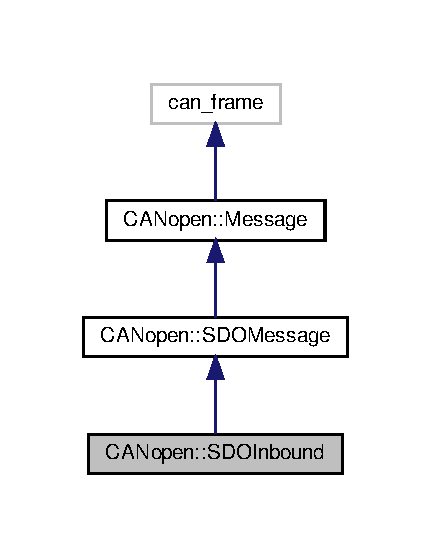
\includegraphics[width=207pt]{class_c_a_nopen_1_1_s_d_o_inbound__inherit__graph}
\end{center}
\end{figure}


Collaboration diagram for C\+A\+Nopen\+:\+:S\+D\+O\+Inbound\+:\nopagebreak
\begin{figure}[H]
\begin{center}
\leavevmode
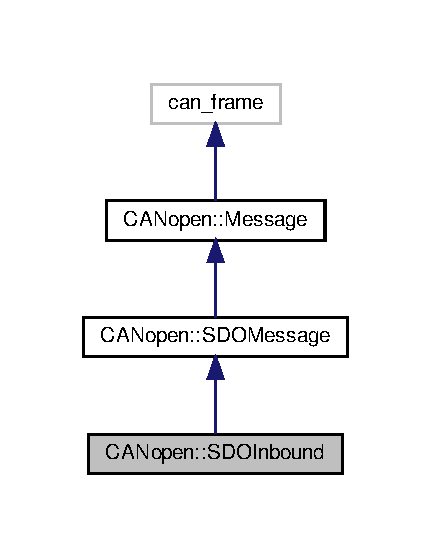
\includegraphics[width=207pt]{class_c_a_nopen_1_1_s_d_o_inbound__coll__graph}
\end{center}
\end{figure}
\subsection*{Public Member Functions}
\begin{DoxyCompactItemize}
\item 
\hyperlink{class_c_a_nopen_1_1_s_d_o_inbound_a9ec2a9d10554f7f47aeaa5d83e048f70}{S\+D\+O\+Inbound} (const can\+\_\+frame \&other)
\end{DoxyCompactItemize}
\subsection*{Additional Inherited Members}


\subsection{Detailed Description}


Definition at line 31 of file sdo.\+h.



\subsection{Constructor \& Destructor Documentation}
\mbox{\Hypertarget{class_c_a_nopen_1_1_s_d_o_inbound_a9ec2a9d10554f7f47aeaa5d83e048f70}\label{class_c_a_nopen_1_1_s_d_o_inbound_a9ec2a9d10554f7f47aeaa5d83e048f70}} 
\index{C\+A\+Nopen\+::\+S\+D\+O\+Inbound@{C\+A\+Nopen\+::\+S\+D\+O\+Inbound}!S\+D\+O\+Inbound@{S\+D\+O\+Inbound}}
\index{S\+D\+O\+Inbound@{S\+D\+O\+Inbound}!C\+A\+Nopen\+::\+S\+D\+O\+Inbound@{C\+A\+Nopen\+::\+S\+D\+O\+Inbound}}
\subsubsection{\texorpdfstring{S\+D\+O\+Inbound()}{SDOInbound()}}
{\footnotesize\ttfamily C\+A\+Nopen\+::\+S\+D\+O\+Inbound\+::\+S\+D\+O\+Inbound (\begin{DoxyParamCaption}\item[{const can\+\_\+frame \&}]{other }\end{DoxyParamCaption})}



Definition at line 32 of file sdo.\+cpp.



The documentation for this class was generated from the following files\+:\begin{DoxyCompactItemize}
\item 
/home/adev/\+Documents/\+S\+T\+E\+C\+H/lxm32/lib/canopen/include/\hyperlink{sdo_8h}{sdo.\+h}\item 
/home/adev/\+Documents/\+S\+T\+E\+C\+H/lxm32/lib/canopen/src/\hyperlink{sdo_8cpp}{sdo.\+cpp}\end{DoxyCompactItemize}

\hypertarget{class_c_a_nopen_1_1_s_d_o_message}{}\section{C\+A\+Nopen\+:\+:S\+D\+O\+Message Class Reference}
\label{class_c_a_nopen_1_1_s_d_o_message}\index{C\+A\+Nopen\+::\+S\+D\+O\+Message@{C\+A\+Nopen\+::\+S\+D\+O\+Message}}


{\ttfamily \#include $<$sdo.\+h$>$}



Inheritance diagram for C\+A\+Nopen\+:\+:S\+D\+O\+Message\+:\nopagebreak
\begin{figure}[H]
\begin{center}
\leavevmode
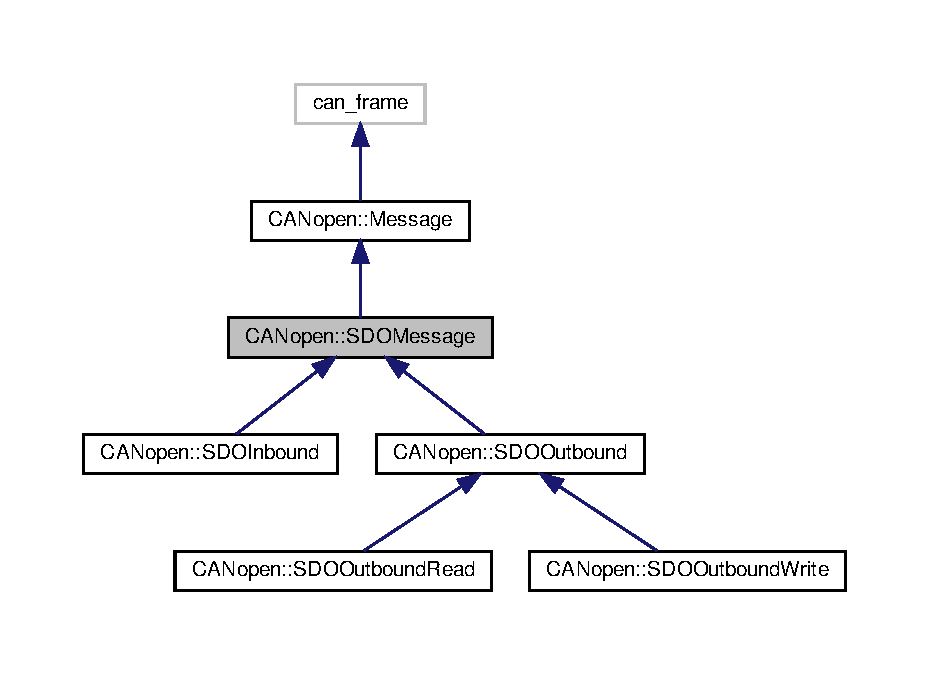
\includegraphics[width=350pt]{class_c_a_nopen_1_1_s_d_o_message__inherit__graph}
\end{center}
\end{figure}


Collaboration diagram for C\+A\+Nopen\+:\+:S\+D\+O\+Message\+:\nopagebreak
\begin{figure}[H]
\begin{center}
\leavevmode
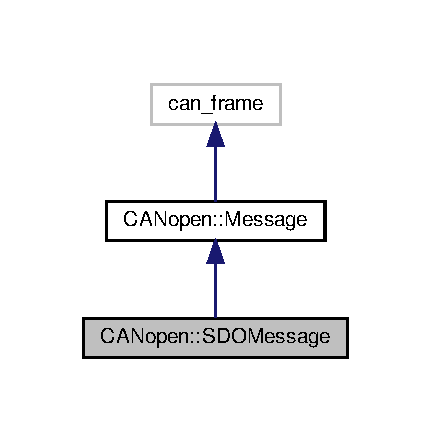
\includegraphics[width=207pt]{class_c_a_nopen_1_1_s_d_o_message__coll__graph}
\end{center}
\end{figure}
\subsection*{Public Types}
\begin{DoxyCompactItemize}
\item 
enum \hyperlink{class_c_a_nopen_1_1_s_d_o_message_aba8926782f1557b8d7d90f430b26cd8d}{R\+D\+WR} \{ \hyperlink{class_c_a_nopen_1_1_s_d_o_message_aba8926782f1557b8d7d90f430b26cd8da289c8fc8152983893c105c7babdc681b}{Read}, 
\hyperlink{class_c_a_nopen_1_1_s_d_o_message_aba8926782f1557b8d7d90f430b26cd8da0583f2eb7789cc0917f023c833e64ea2}{Write}
 \}
\item 
enum \hyperlink{class_c_a_nopen_1_1_s_d_o_message_a87e867140acb008777fb9419626d19ea}{C\+CS} \{ \newline
\hyperlink{class_c_a_nopen_1_1_s_d_o_message_a87e867140acb008777fb9419626d19eaa44e7a57deaad302a380a06c5788f780f}{Segment\+Download} = 0, 
\hyperlink{class_c_a_nopen_1_1_s_d_o_message_a87e867140acb008777fb9419626d19eaa78901951e33e3579cb856b53609248fe}{Initiate\+Download} = 1, 
\hyperlink{class_c_a_nopen_1_1_s_d_o_message_a87e867140acb008777fb9419626d19eaaf330c9070f66925edbece3a896f4c0e3}{Initiate\+Upload} = 2, 
\hyperlink{class_c_a_nopen_1_1_s_d_o_message_a87e867140acb008777fb9419626d19eaaebae2db15a511c989cfa09218d3858f9}{Segment\+Upload} = 3, 
\newline
\hyperlink{class_c_a_nopen_1_1_s_d_o_message_a87e867140acb008777fb9419626d19eaa211ad465c11d2bac3504d46fdc020954}{Abort\+Transfer} = 4, 
\hyperlink{class_c_a_nopen_1_1_s_d_o_message_a87e867140acb008777fb9419626d19eaab1dec130d95dc1c743b8d87dd56b8d7f}{Block\+Upload} = 5, 
\hyperlink{class_c_a_nopen_1_1_s_d_o_message_a87e867140acb008777fb9419626d19eaade0ce8477f2b012117aa5fa6c2c10479}{Block\+Download} = 6
 \}
\end{DoxyCompactItemize}
\subsection*{Public Member Functions}
\begin{DoxyCompactItemize}
\item 
\hyperlink{class_c_a_nopen_1_1_s_d_o_message_a6229048c08585beeb1e19d76ae0966cd}{S\+D\+O\+Message} ()=default
\item 
\hyperlink{class_c_a_nopen_1_1_s_d_o_message_a73ab5aad06fd6a6f53fb614f4d9a8465}{S\+D\+O\+Message} (const can\+\_\+frame \&other)
\item 
\hyperlink{class_c_a_nopen_1_1_s_d_o_message_ad299429ca0de823d392fb24addf4fe85}{S\+D\+O\+Message} (\hyperlink{class_c_a_nopen_1_1_message_a0f8f95e4ea1284011cd122629edc5468}{Function\+Code} fn, uint8\+\_\+t \hyperlink{class_c_a_nopen_1_1_message_a845fe0c7682bd6eeef0a5dd87b5e3c63}{node\+\_\+id}, \hyperlink{class_c_a_nopen_1_1_s_d_o_message_a87e867140acb008777fb9419626d19ea}{C\+CS} spec, uint8\+\_\+t n, uint8\+\_\+t e, uint8\+\_\+t s, uint16\+\_\+t index, uint8\+\_\+t subindex, \hyperlink{class_c_a_nopen_1_1_payload}{Payload} \hyperlink{class_c_a_nopen_1_1_s_d_o_message_a051509ddb3a59dfe066f9d90c80c2eec}{payload})
\item 
\hyperlink{class_c_a_nopen_1_1_payload}{Payload} \hyperlink{class_c_a_nopen_1_1_s_d_o_message_a051509ddb3a59dfe066f9d90c80c2eec}{payload} ()
\end{DoxyCompactItemize}


\subsection{Detailed Description}


Definition at line 7 of file sdo.\+h.



\subsection{Member Enumeration Documentation}
\mbox{\Hypertarget{class_c_a_nopen_1_1_s_d_o_message_a87e867140acb008777fb9419626d19ea}\label{class_c_a_nopen_1_1_s_d_o_message_a87e867140acb008777fb9419626d19ea}} 
\index{C\+A\+Nopen\+::\+S\+D\+O\+Message@{C\+A\+Nopen\+::\+S\+D\+O\+Message}!C\+CS@{C\+CS}}
\index{C\+CS@{C\+CS}!C\+A\+Nopen\+::\+S\+D\+O\+Message@{C\+A\+Nopen\+::\+S\+D\+O\+Message}}
\subsubsection{\texorpdfstring{C\+CS}{CCS}}
{\footnotesize\ttfamily enum \hyperlink{class_c_a_nopen_1_1_s_d_o_message_a87e867140acb008777fb9419626d19ea}{C\+A\+Nopen\+::\+S\+D\+O\+Message\+::\+C\+CS}}

\begin{DoxyEnumFields}{Enumerator}
\raisebox{\heightof{T}}[0pt][0pt]{\index{Segment\+Download@{Segment\+Download}!C\+A\+Nopen\+::\+S\+D\+O\+Message@{C\+A\+Nopen\+::\+S\+D\+O\+Message}}\index{C\+A\+Nopen\+::\+S\+D\+O\+Message@{C\+A\+Nopen\+::\+S\+D\+O\+Message}!Segment\+Download@{Segment\+Download}}}\mbox{\Hypertarget{class_c_a_nopen_1_1_s_d_o_message_a87e867140acb008777fb9419626d19eaa44e7a57deaad302a380a06c5788f780f}\label{class_c_a_nopen_1_1_s_d_o_message_a87e867140acb008777fb9419626d19eaa44e7a57deaad302a380a06c5788f780f}} 
Segment\+Download&\\
\hline

\raisebox{\heightof{T}}[0pt][0pt]{\index{Initiate\+Download@{Initiate\+Download}!C\+A\+Nopen\+::\+S\+D\+O\+Message@{C\+A\+Nopen\+::\+S\+D\+O\+Message}}\index{C\+A\+Nopen\+::\+S\+D\+O\+Message@{C\+A\+Nopen\+::\+S\+D\+O\+Message}!Initiate\+Download@{Initiate\+Download}}}\mbox{\Hypertarget{class_c_a_nopen_1_1_s_d_o_message_a87e867140acb008777fb9419626d19eaa78901951e33e3579cb856b53609248fe}\label{class_c_a_nopen_1_1_s_d_o_message_a87e867140acb008777fb9419626d19eaa78901951e33e3579cb856b53609248fe}} 
Initiate\+Download&\\
\hline

\raisebox{\heightof{T}}[0pt][0pt]{\index{Initiate\+Upload@{Initiate\+Upload}!C\+A\+Nopen\+::\+S\+D\+O\+Message@{C\+A\+Nopen\+::\+S\+D\+O\+Message}}\index{C\+A\+Nopen\+::\+S\+D\+O\+Message@{C\+A\+Nopen\+::\+S\+D\+O\+Message}!Initiate\+Upload@{Initiate\+Upload}}}\mbox{\Hypertarget{class_c_a_nopen_1_1_s_d_o_message_a87e867140acb008777fb9419626d19eaaf330c9070f66925edbece3a896f4c0e3}\label{class_c_a_nopen_1_1_s_d_o_message_a87e867140acb008777fb9419626d19eaaf330c9070f66925edbece3a896f4c0e3}} 
Initiate\+Upload&\\
\hline

\raisebox{\heightof{T}}[0pt][0pt]{\index{Segment\+Upload@{Segment\+Upload}!C\+A\+Nopen\+::\+S\+D\+O\+Message@{C\+A\+Nopen\+::\+S\+D\+O\+Message}}\index{C\+A\+Nopen\+::\+S\+D\+O\+Message@{C\+A\+Nopen\+::\+S\+D\+O\+Message}!Segment\+Upload@{Segment\+Upload}}}\mbox{\Hypertarget{class_c_a_nopen_1_1_s_d_o_message_a87e867140acb008777fb9419626d19eaaebae2db15a511c989cfa09218d3858f9}\label{class_c_a_nopen_1_1_s_d_o_message_a87e867140acb008777fb9419626d19eaaebae2db15a511c989cfa09218d3858f9}} 
Segment\+Upload&\\
\hline

\raisebox{\heightof{T}}[0pt][0pt]{\index{Abort\+Transfer@{Abort\+Transfer}!C\+A\+Nopen\+::\+S\+D\+O\+Message@{C\+A\+Nopen\+::\+S\+D\+O\+Message}}\index{C\+A\+Nopen\+::\+S\+D\+O\+Message@{C\+A\+Nopen\+::\+S\+D\+O\+Message}!Abort\+Transfer@{Abort\+Transfer}}}\mbox{\Hypertarget{class_c_a_nopen_1_1_s_d_o_message_a87e867140acb008777fb9419626d19eaa211ad465c11d2bac3504d46fdc020954}\label{class_c_a_nopen_1_1_s_d_o_message_a87e867140acb008777fb9419626d19eaa211ad465c11d2bac3504d46fdc020954}} 
Abort\+Transfer&\\
\hline

\raisebox{\heightof{T}}[0pt][0pt]{\index{Block\+Upload@{Block\+Upload}!C\+A\+Nopen\+::\+S\+D\+O\+Message@{C\+A\+Nopen\+::\+S\+D\+O\+Message}}\index{C\+A\+Nopen\+::\+S\+D\+O\+Message@{C\+A\+Nopen\+::\+S\+D\+O\+Message}!Block\+Upload@{Block\+Upload}}}\mbox{\Hypertarget{class_c_a_nopen_1_1_s_d_o_message_a87e867140acb008777fb9419626d19eaab1dec130d95dc1c743b8d87dd56b8d7f}\label{class_c_a_nopen_1_1_s_d_o_message_a87e867140acb008777fb9419626d19eaab1dec130d95dc1c743b8d87dd56b8d7f}} 
Block\+Upload&\\
\hline

\raisebox{\heightof{T}}[0pt][0pt]{\index{Block\+Download@{Block\+Download}!C\+A\+Nopen\+::\+S\+D\+O\+Message@{C\+A\+Nopen\+::\+S\+D\+O\+Message}}\index{C\+A\+Nopen\+::\+S\+D\+O\+Message@{C\+A\+Nopen\+::\+S\+D\+O\+Message}!Block\+Download@{Block\+Download}}}\mbox{\Hypertarget{class_c_a_nopen_1_1_s_d_o_message_a87e867140acb008777fb9419626d19eaade0ce8477f2b012117aa5fa6c2c10479}\label{class_c_a_nopen_1_1_s_d_o_message_a87e867140acb008777fb9419626d19eaade0ce8477f2b012117aa5fa6c2c10479}} 
Block\+Download&\\
\hline

\end{DoxyEnumFields}


Definition at line 14 of file sdo.\+h.

\mbox{\Hypertarget{class_c_a_nopen_1_1_s_d_o_message_aba8926782f1557b8d7d90f430b26cd8d}\label{class_c_a_nopen_1_1_s_d_o_message_aba8926782f1557b8d7d90f430b26cd8d}} 
\index{C\+A\+Nopen\+::\+S\+D\+O\+Message@{C\+A\+Nopen\+::\+S\+D\+O\+Message}!R\+D\+WR@{R\+D\+WR}}
\index{R\+D\+WR@{R\+D\+WR}!C\+A\+Nopen\+::\+S\+D\+O\+Message@{C\+A\+Nopen\+::\+S\+D\+O\+Message}}
\subsubsection{\texorpdfstring{R\+D\+WR}{RDWR}}
{\footnotesize\ttfamily enum \hyperlink{class_c_a_nopen_1_1_s_d_o_message_aba8926782f1557b8d7d90f430b26cd8d}{C\+A\+Nopen\+::\+S\+D\+O\+Message\+::\+R\+D\+WR}}

\begin{DoxyEnumFields}{Enumerator}
\raisebox{\heightof{T}}[0pt][0pt]{\index{Read@{Read}!C\+A\+Nopen\+::\+S\+D\+O\+Message@{C\+A\+Nopen\+::\+S\+D\+O\+Message}}\index{C\+A\+Nopen\+::\+S\+D\+O\+Message@{C\+A\+Nopen\+::\+S\+D\+O\+Message}!Read@{Read}}}\mbox{\Hypertarget{class_c_a_nopen_1_1_s_d_o_message_aba8926782f1557b8d7d90f430b26cd8da289c8fc8152983893c105c7babdc681b}\label{class_c_a_nopen_1_1_s_d_o_message_aba8926782f1557b8d7d90f430b26cd8da289c8fc8152983893c105c7babdc681b}} 
Read&\\
\hline

\raisebox{\heightof{T}}[0pt][0pt]{\index{Write@{Write}!C\+A\+Nopen\+::\+S\+D\+O\+Message@{C\+A\+Nopen\+::\+S\+D\+O\+Message}}\index{C\+A\+Nopen\+::\+S\+D\+O\+Message@{C\+A\+Nopen\+::\+S\+D\+O\+Message}!Write@{Write}}}\mbox{\Hypertarget{class_c_a_nopen_1_1_s_d_o_message_aba8926782f1557b8d7d90f430b26cd8da0583f2eb7789cc0917f023c833e64ea2}\label{class_c_a_nopen_1_1_s_d_o_message_aba8926782f1557b8d7d90f430b26cd8da0583f2eb7789cc0917f023c833e64ea2}} 
Write&\\
\hline

\end{DoxyEnumFields}


Definition at line 9 of file sdo.\+h.



\subsection{Constructor \& Destructor Documentation}
\mbox{\Hypertarget{class_c_a_nopen_1_1_s_d_o_message_a6229048c08585beeb1e19d76ae0966cd}\label{class_c_a_nopen_1_1_s_d_o_message_a6229048c08585beeb1e19d76ae0966cd}} 
\index{C\+A\+Nopen\+::\+S\+D\+O\+Message@{C\+A\+Nopen\+::\+S\+D\+O\+Message}!S\+D\+O\+Message@{S\+D\+O\+Message}}
\index{S\+D\+O\+Message@{S\+D\+O\+Message}!C\+A\+Nopen\+::\+S\+D\+O\+Message@{C\+A\+Nopen\+::\+S\+D\+O\+Message}}
\subsubsection{\texorpdfstring{S\+D\+O\+Message()}{SDOMessage()}\hspace{0.1cm}{\footnotesize\ttfamily [1/3]}}
{\footnotesize\ttfamily C\+A\+Nopen\+::\+S\+D\+O\+Message\+::\+S\+D\+O\+Message (\begin{DoxyParamCaption}{ }\end{DoxyParamCaption})\hspace{0.3cm}{\ttfamily [default]}}

\mbox{\Hypertarget{class_c_a_nopen_1_1_s_d_o_message_a73ab5aad06fd6a6f53fb614f4d9a8465}\label{class_c_a_nopen_1_1_s_d_o_message_a73ab5aad06fd6a6f53fb614f4d9a8465}} 
\index{C\+A\+Nopen\+::\+S\+D\+O\+Message@{C\+A\+Nopen\+::\+S\+D\+O\+Message}!S\+D\+O\+Message@{S\+D\+O\+Message}}
\index{S\+D\+O\+Message@{S\+D\+O\+Message}!C\+A\+Nopen\+::\+S\+D\+O\+Message@{C\+A\+Nopen\+::\+S\+D\+O\+Message}}
\subsubsection{\texorpdfstring{S\+D\+O\+Message()}{SDOMessage()}\hspace{0.1cm}{\footnotesize\ttfamily [2/3]}}
{\footnotesize\ttfamily C\+A\+Nopen\+::\+S\+D\+O\+Message\+::\+S\+D\+O\+Message (\begin{DoxyParamCaption}\item[{const can\+\_\+frame \&}]{other }\end{DoxyParamCaption})}



Definition at line 6 of file sdo.\+cpp.

\mbox{\Hypertarget{class_c_a_nopen_1_1_s_d_o_message_ad299429ca0de823d392fb24addf4fe85}\label{class_c_a_nopen_1_1_s_d_o_message_ad299429ca0de823d392fb24addf4fe85}} 
\index{C\+A\+Nopen\+::\+S\+D\+O\+Message@{C\+A\+Nopen\+::\+S\+D\+O\+Message}!S\+D\+O\+Message@{S\+D\+O\+Message}}
\index{S\+D\+O\+Message@{S\+D\+O\+Message}!C\+A\+Nopen\+::\+S\+D\+O\+Message@{C\+A\+Nopen\+::\+S\+D\+O\+Message}}
\subsubsection{\texorpdfstring{S\+D\+O\+Message()}{SDOMessage()}\hspace{0.1cm}{\footnotesize\ttfamily [3/3]}}
{\footnotesize\ttfamily C\+A\+Nopen\+::\+S\+D\+O\+Message\+::\+S\+D\+O\+Message (\begin{DoxyParamCaption}\item[{\hyperlink{class_c_a_nopen_1_1_message_a0f8f95e4ea1284011cd122629edc5468}{Function\+Code}}]{fn,  }\item[{uint8\+\_\+t}]{node\+\_\+id,  }\item[{\hyperlink{class_c_a_nopen_1_1_s_d_o_message_a87e867140acb008777fb9419626d19ea}{C\+CS}}]{spec,  }\item[{uint8\+\_\+t}]{n,  }\item[{uint8\+\_\+t}]{e,  }\item[{uint8\+\_\+t}]{s,  }\item[{uint16\+\_\+t}]{index,  }\item[{uint8\+\_\+t}]{subindex,  }\item[{\hyperlink{class_c_a_nopen_1_1_payload}{Payload}}]{payload }\end{DoxyParamCaption})}



Definition at line 10 of file sdo.\+cpp.



\subsection{Member Function Documentation}
\mbox{\Hypertarget{class_c_a_nopen_1_1_s_d_o_message_a051509ddb3a59dfe066f9d90c80c2eec}\label{class_c_a_nopen_1_1_s_d_o_message_a051509ddb3a59dfe066f9d90c80c2eec}} 
\index{C\+A\+Nopen\+::\+S\+D\+O\+Message@{C\+A\+Nopen\+::\+S\+D\+O\+Message}!payload@{payload}}
\index{payload@{payload}!C\+A\+Nopen\+::\+S\+D\+O\+Message@{C\+A\+Nopen\+::\+S\+D\+O\+Message}}
\subsubsection{\texorpdfstring{payload()}{payload()}}
{\footnotesize\ttfamily \hyperlink{class_c_a_nopen_1_1_payload}{Payload} C\+A\+Nopen\+::\+S\+D\+O\+Message\+::payload (\begin{DoxyParamCaption}{ }\end{DoxyParamCaption})}



Definition at line 28 of file sdo.\+cpp.



The documentation for this class was generated from the following files\+:\begin{DoxyCompactItemize}
\item 
/home/adev/\+Documents/\+S\+T\+E\+C\+H/lxm32/lib/canopen/include/\hyperlink{sdo_8h}{sdo.\+h}\item 
/home/adev/\+Documents/\+S\+T\+E\+C\+H/lxm32/lib/canopen/src/\hyperlink{sdo_8cpp}{sdo.\+cpp}\end{DoxyCompactItemize}

\hypertarget{class_c_a_nopen_1_1_s_d_o_outbound}{}\section{C\+A\+Nopen\+:\+:S\+D\+O\+Outbound Class Reference}
\label{class_c_a_nopen_1_1_s_d_o_outbound}\index{C\+A\+Nopen\+::\+S\+D\+O\+Outbound@{C\+A\+Nopen\+::\+S\+D\+O\+Outbound}}


{\ttfamily \#include $<$sdo.\+h$>$}



Inheritance diagram for C\+A\+Nopen\+:\+:S\+D\+O\+Outbound\+:\nopagebreak
\begin{figure}[H]
\begin{center}
\leavevmode
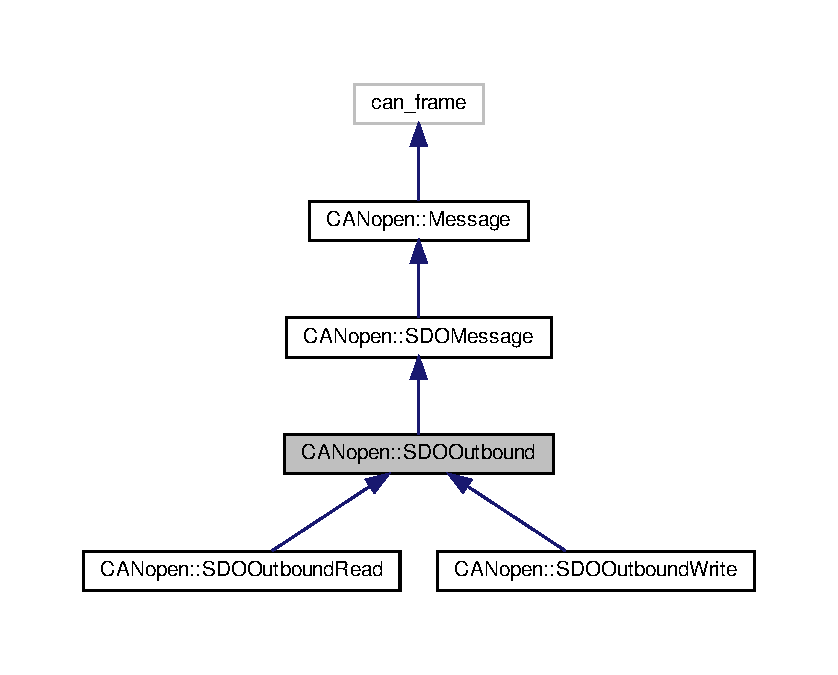
\includegraphics[width=350pt]{class_c_a_nopen_1_1_s_d_o_outbound__inherit__graph}
\end{center}
\end{figure}


Collaboration diagram for C\+A\+Nopen\+:\+:S\+D\+O\+Outbound\+:\nopagebreak
\begin{figure}[H]
\begin{center}
\leavevmode
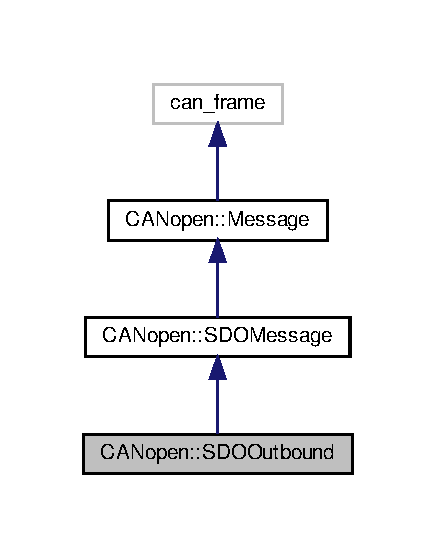
\includegraphics[width=209pt]{class_c_a_nopen_1_1_s_d_o_outbound__coll__graph}
\end{center}
\end{figure}
\subsection*{Public Member Functions}
\begin{DoxyCompactItemize}
\item 
\hyperlink{class_c_a_nopen_1_1_s_d_o_outbound_ac43a44aaaa9356e3ddab74d008c5a3ca}{S\+D\+O\+Outbound} (uint8\+\_\+t \hyperlink{class_c_a_nopen_1_1_message_a845fe0c7682bd6eeef0a5dd87b5e3c63}{node\+\_\+id}, \hyperlink{class_c_a_nopen_1_1_s_d_o_message_aba8926782f1557b8d7d90f430b26cd8d}{R\+D\+WR} dir, uint16\+\_\+t index, uint8\+\_\+t subindex, \hyperlink{class_c_a_nopen_1_1_payload}{Payload} \hyperlink{class_c_a_nopen_1_1_s_d_o_message_a051509ddb3a59dfe066f9d90c80c2eec}{payload})
\end{DoxyCompactItemize}
\subsection*{Additional Inherited Members}


\subsection{Detailed Description}


Definition at line 36 of file sdo.\+h.



\subsection{Constructor \& Destructor Documentation}
\mbox{\Hypertarget{class_c_a_nopen_1_1_s_d_o_outbound_ac43a44aaaa9356e3ddab74d008c5a3ca}\label{class_c_a_nopen_1_1_s_d_o_outbound_ac43a44aaaa9356e3ddab74d008c5a3ca}} 
\index{C\+A\+Nopen\+::\+S\+D\+O\+Outbound@{C\+A\+Nopen\+::\+S\+D\+O\+Outbound}!S\+D\+O\+Outbound@{S\+D\+O\+Outbound}}
\index{S\+D\+O\+Outbound@{S\+D\+O\+Outbound}!C\+A\+Nopen\+::\+S\+D\+O\+Outbound@{C\+A\+Nopen\+::\+S\+D\+O\+Outbound}}
\subsubsection{\texorpdfstring{S\+D\+O\+Outbound()}{SDOOutbound()}}
{\footnotesize\ttfamily C\+A\+Nopen\+::\+S\+D\+O\+Outbound\+::\+S\+D\+O\+Outbound (\begin{DoxyParamCaption}\item[{uint8\+\_\+t}]{node\+\_\+id,  }\item[{\hyperlink{class_c_a_nopen_1_1_s_d_o_message_aba8926782f1557b8d7d90f430b26cd8d}{R\+D\+WR}}]{dir,  }\item[{uint16\+\_\+t}]{index,  }\item[{uint8\+\_\+t}]{subindex,  }\item[{\hyperlink{class_c_a_nopen_1_1_payload}{Payload}}]{payload }\end{DoxyParamCaption})}



Definition at line 36 of file sdo.\+cpp.



The documentation for this class was generated from the following files\+:\begin{DoxyCompactItemize}
\item 
/home/adev/\+Documents/\+S\+T\+E\+C\+H/lxm32/lib/canopen/include/\hyperlink{sdo_8h}{sdo.\+h}\item 
/home/adev/\+Documents/\+S\+T\+E\+C\+H/lxm32/lib/canopen/src/\hyperlink{sdo_8cpp}{sdo.\+cpp}\end{DoxyCompactItemize}

\hypertarget{class_c_a_nopen_1_1_s_d_o_outbound_read}{}\section{C\+A\+Nopen\+:\+:S\+D\+O\+Outbound\+Read Class Reference}
\label{class_c_a_nopen_1_1_s_d_o_outbound_read}\index{C\+A\+Nopen\+::\+S\+D\+O\+Outbound\+Read@{C\+A\+Nopen\+::\+S\+D\+O\+Outbound\+Read}}


{\ttfamily \#include $<$sdo.\+h$>$}



Inheritance diagram for C\+A\+Nopen\+:\+:S\+D\+O\+Outbound\+Read\+:\nopagebreak
\begin{figure}[H]
\begin{center}
\leavevmode
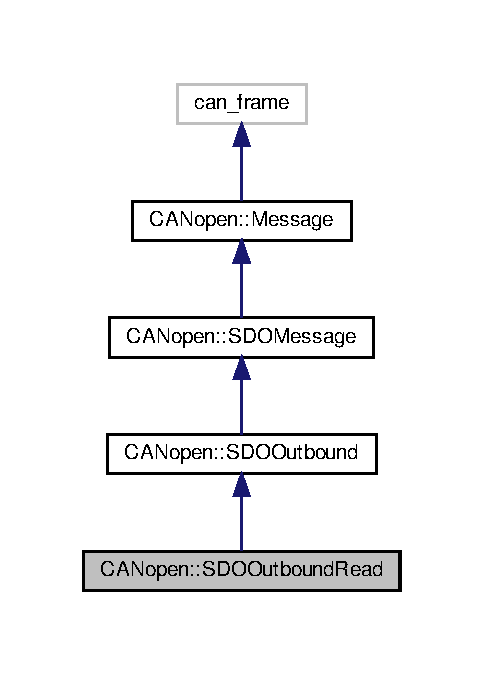
\includegraphics[width=232pt]{class_c_a_nopen_1_1_s_d_o_outbound_read__inherit__graph}
\end{center}
\end{figure}


Collaboration diagram for C\+A\+Nopen\+:\+:S\+D\+O\+Outbound\+Read\+:\nopagebreak
\begin{figure}[H]
\begin{center}
\leavevmode
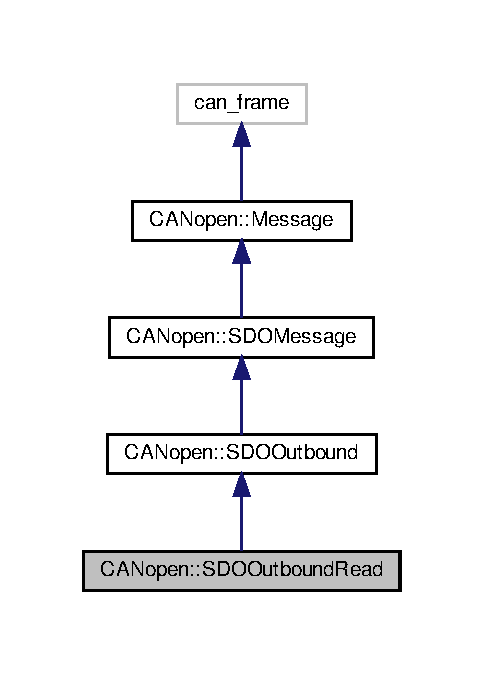
\includegraphics[width=232pt]{class_c_a_nopen_1_1_s_d_o_outbound_read__coll__graph}
\end{center}
\end{figure}
\subsection*{Public Member Functions}
\begin{DoxyCompactItemize}
\item 
\hyperlink{class_c_a_nopen_1_1_s_d_o_outbound_read_a622eb7aa4300ebdcd74d7e50e5a7b6e3}{S\+D\+O\+Outbound\+Read} (uint8\+\_\+t \hyperlink{class_c_a_nopen_1_1_message_a845fe0c7682bd6eeef0a5dd87b5e3c63}{node\+\_\+id}, uint16\+\_\+t index, uint8\+\_\+t subindex)
\item 
\hyperlink{class_c_a_nopen_1_1_s_d_o_outbound_read_a888154f4196096357dad341b131ee81f}{S\+D\+O\+Outbound\+Read} (uint8\+\_\+t \hyperlink{class_c_a_nopen_1_1_message_a845fe0c7682bd6eeef0a5dd87b5e3c63}{node\+\_\+id}, uint32\+\_\+t index\+\_\+\+\_\+sub)
\end{DoxyCompactItemize}
\subsection*{Additional Inherited Members}


\subsection{Detailed Description}


Definition at line 41 of file sdo.\+h.



\subsection{Constructor \& Destructor Documentation}
\mbox{\Hypertarget{class_c_a_nopen_1_1_s_d_o_outbound_read_a622eb7aa4300ebdcd74d7e50e5a7b6e3}\label{class_c_a_nopen_1_1_s_d_o_outbound_read_a622eb7aa4300ebdcd74d7e50e5a7b6e3}} 
\index{C\+A\+Nopen\+::\+S\+D\+O\+Outbound\+Read@{C\+A\+Nopen\+::\+S\+D\+O\+Outbound\+Read}!S\+D\+O\+Outbound\+Read@{S\+D\+O\+Outbound\+Read}}
\index{S\+D\+O\+Outbound\+Read@{S\+D\+O\+Outbound\+Read}!C\+A\+Nopen\+::\+S\+D\+O\+Outbound\+Read@{C\+A\+Nopen\+::\+S\+D\+O\+Outbound\+Read}}
\subsubsection{\texorpdfstring{S\+D\+O\+Outbound\+Read()}{SDOOutboundRead()}\hspace{0.1cm}{\footnotesize\ttfamily [1/2]}}
{\footnotesize\ttfamily C\+A\+Nopen\+::\+S\+D\+O\+Outbound\+Read\+::\+S\+D\+O\+Outbound\+Read (\begin{DoxyParamCaption}\item[{uint8\+\_\+t}]{node\+\_\+id,  }\item[{uint16\+\_\+t}]{index,  }\item[{uint8\+\_\+t}]{subindex }\end{DoxyParamCaption})}



Definition at line 40 of file sdo.\+cpp.

\mbox{\Hypertarget{class_c_a_nopen_1_1_s_d_o_outbound_read_a888154f4196096357dad341b131ee81f}\label{class_c_a_nopen_1_1_s_d_o_outbound_read_a888154f4196096357dad341b131ee81f}} 
\index{C\+A\+Nopen\+::\+S\+D\+O\+Outbound\+Read@{C\+A\+Nopen\+::\+S\+D\+O\+Outbound\+Read}!S\+D\+O\+Outbound\+Read@{S\+D\+O\+Outbound\+Read}}
\index{S\+D\+O\+Outbound\+Read@{S\+D\+O\+Outbound\+Read}!C\+A\+Nopen\+::\+S\+D\+O\+Outbound\+Read@{C\+A\+Nopen\+::\+S\+D\+O\+Outbound\+Read}}
\subsubsection{\texorpdfstring{S\+D\+O\+Outbound\+Read()}{SDOOutboundRead()}\hspace{0.1cm}{\footnotesize\ttfamily [2/2]}}
{\footnotesize\ttfamily C\+A\+Nopen\+::\+S\+D\+O\+Outbound\+Read\+::\+S\+D\+O\+Outbound\+Read (\begin{DoxyParamCaption}\item[{uint8\+\_\+t}]{node\+\_\+id,  }\item[{uint32\+\_\+t}]{index\+\_\+\+\_\+sub }\end{DoxyParamCaption})}



Definition at line 44 of file sdo.\+cpp.



The documentation for this class was generated from the following files\+:\begin{DoxyCompactItemize}
\item 
/home/adev/\+Documents/\+S\+T\+E\+C\+H/lxm32/lib/canopen/include/\hyperlink{sdo_8h}{sdo.\+h}\item 
/home/adev/\+Documents/\+S\+T\+E\+C\+H/lxm32/lib/canopen/src/\hyperlink{sdo_8cpp}{sdo.\+cpp}\end{DoxyCompactItemize}

\hypertarget{class_c_a_nopen_1_1_s_d_o_outbound_write}{}\section{C\+A\+Nopen\+:\+:S\+D\+O\+Outbound\+Write Class Reference}
\label{class_c_a_nopen_1_1_s_d_o_outbound_write}\index{C\+A\+Nopen\+::\+S\+D\+O\+Outbound\+Write@{C\+A\+Nopen\+::\+S\+D\+O\+Outbound\+Write}}


{\ttfamily \#include $<$sdo.\+h$>$}



Inheritance diagram for C\+A\+Nopen\+:\+:S\+D\+O\+Outbound\+Write\+:\nopagebreak
\begin{figure}[H]
\begin{center}
\leavevmode
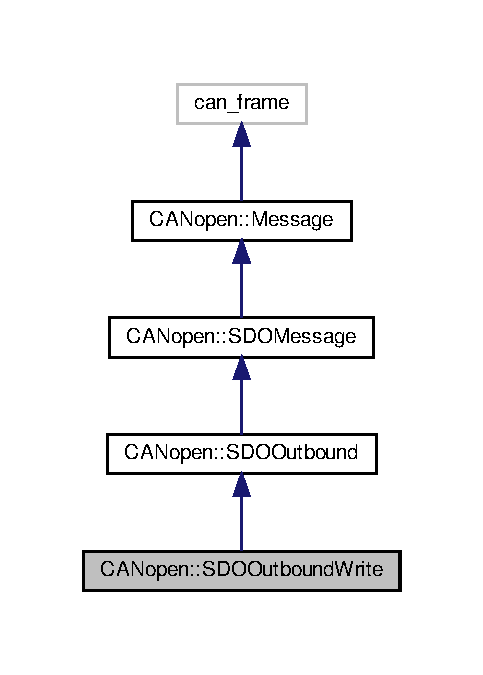
\includegraphics[width=232pt]{class_c_a_nopen_1_1_s_d_o_outbound_write__inherit__graph}
\end{center}
\end{figure}


Collaboration diagram for C\+A\+Nopen\+:\+:S\+D\+O\+Outbound\+Write\+:\nopagebreak
\begin{figure}[H]
\begin{center}
\leavevmode
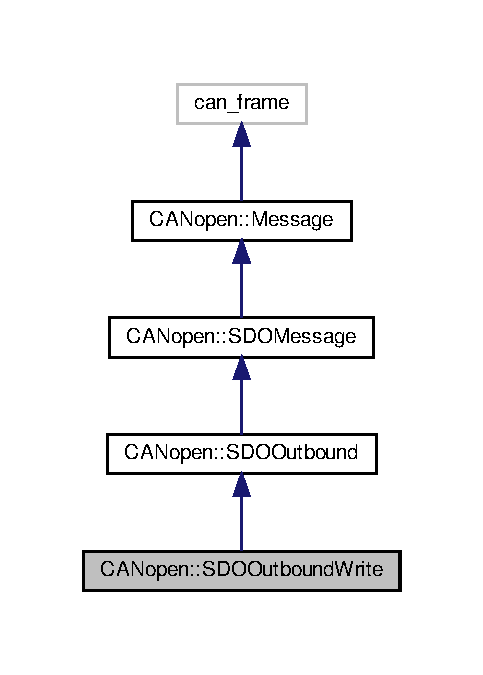
\includegraphics[width=232pt]{class_c_a_nopen_1_1_s_d_o_outbound_write__coll__graph}
\end{center}
\end{figure}
\subsection*{Public Member Functions}
\begin{DoxyCompactItemize}
\item 
\hyperlink{class_c_a_nopen_1_1_s_d_o_outbound_write_af86ced7cb745cc3b18c4cd7c1406a312}{S\+D\+O\+Outbound\+Write} (uint8\+\_\+t \hyperlink{class_c_a_nopen_1_1_message_a845fe0c7682bd6eeef0a5dd87b5e3c63}{node\+\_\+id}, uint16\+\_\+t index, uint8\+\_\+t subindex, \hyperlink{class_c_a_nopen_1_1_payload}{Payload} \hyperlink{class_c_a_nopen_1_1_s_d_o_message_a051509ddb3a59dfe066f9d90c80c2eec}{payload})
\item 
\hyperlink{class_c_a_nopen_1_1_s_d_o_outbound_write_a7c71af3977530091cafdc6aeae6f6c6a}{S\+D\+O\+Outbound\+Write} (uint8\+\_\+t \hyperlink{class_c_a_nopen_1_1_message_a845fe0c7682bd6eeef0a5dd87b5e3c63}{node\+\_\+id}, uint32\+\_\+t index\+\_\+\+\_\+sub, \hyperlink{class_c_a_nopen_1_1_payload}{Payload} \hyperlink{class_c_a_nopen_1_1_s_d_o_message_a051509ddb3a59dfe066f9d90c80c2eec}{payload})
\end{DoxyCompactItemize}
\subsection*{Additional Inherited Members}


\subsection{Detailed Description}


Definition at line 47 of file sdo.\+h.



\subsection{Constructor \& Destructor Documentation}
\mbox{\Hypertarget{class_c_a_nopen_1_1_s_d_o_outbound_write_af86ced7cb745cc3b18c4cd7c1406a312}\label{class_c_a_nopen_1_1_s_d_o_outbound_write_af86ced7cb745cc3b18c4cd7c1406a312}} 
\index{C\+A\+Nopen\+::\+S\+D\+O\+Outbound\+Write@{C\+A\+Nopen\+::\+S\+D\+O\+Outbound\+Write}!S\+D\+O\+Outbound\+Write@{S\+D\+O\+Outbound\+Write}}
\index{S\+D\+O\+Outbound\+Write@{S\+D\+O\+Outbound\+Write}!C\+A\+Nopen\+::\+S\+D\+O\+Outbound\+Write@{C\+A\+Nopen\+::\+S\+D\+O\+Outbound\+Write}}
\subsubsection{\texorpdfstring{S\+D\+O\+Outbound\+Write()}{SDOOutboundWrite()}\hspace{0.1cm}{\footnotesize\ttfamily [1/2]}}
{\footnotesize\ttfamily C\+A\+Nopen\+::\+S\+D\+O\+Outbound\+Write\+::\+S\+D\+O\+Outbound\+Write (\begin{DoxyParamCaption}\item[{uint8\+\_\+t}]{node\+\_\+id,  }\item[{uint16\+\_\+t}]{index,  }\item[{uint8\+\_\+t}]{subindex,  }\item[{\hyperlink{class_c_a_nopen_1_1_payload}{Payload}}]{payload }\end{DoxyParamCaption})}



Definition at line 48 of file sdo.\+cpp.

\mbox{\Hypertarget{class_c_a_nopen_1_1_s_d_o_outbound_write_a7c71af3977530091cafdc6aeae6f6c6a}\label{class_c_a_nopen_1_1_s_d_o_outbound_write_a7c71af3977530091cafdc6aeae6f6c6a}} 
\index{C\+A\+Nopen\+::\+S\+D\+O\+Outbound\+Write@{C\+A\+Nopen\+::\+S\+D\+O\+Outbound\+Write}!S\+D\+O\+Outbound\+Write@{S\+D\+O\+Outbound\+Write}}
\index{S\+D\+O\+Outbound\+Write@{S\+D\+O\+Outbound\+Write}!C\+A\+Nopen\+::\+S\+D\+O\+Outbound\+Write@{C\+A\+Nopen\+::\+S\+D\+O\+Outbound\+Write}}
\subsubsection{\texorpdfstring{S\+D\+O\+Outbound\+Write()}{SDOOutboundWrite()}\hspace{0.1cm}{\footnotesize\ttfamily [2/2]}}
{\footnotesize\ttfamily C\+A\+Nopen\+::\+S\+D\+O\+Outbound\+Write\+::\+S\+D\+O\+Outbound\+Write (\begin{DoxyParamCaption}\item[{uint8\+\_\+t}]{node\+\_\+id,  }\item[{uint32\+\_\+t}]{index\+\_\+\+\_\+sub,  }\item[{\hyperlink{class_c_a_nopen_1_1_payload}{Payload}}]{payload }\end{DoxyParamCaption})}



Definition at line 52 of file sdo.\+cpp.



The documentation for this class was generated from the following files\+:\begin{DoxyCompactItemize}
\item 
/home/adev/\+Documents/\+S\+T\+E\+C\+H/lxm32/lib/canopen/include/\hyperlink{sdo_8h}{sdo.\+h}\item 
/home/adev/\+Documents/\+S\+T\+E\+C\+H/lxm32/lib/canopen/src/\hyperlink{sdo_8cpp}{sdo.\+cpp}\end{DoxyCompactItemize}

\hypertarget{class_c_a_nopen_1_1_socket}{}\section{C\+A\+Nopen\+:\+:Socket Class Reference}
\label{class_c_a_nopen_1_1_socket}\index{C\+A\+Nopen\+::\+Socket@{C\+A\+Nopen\+::\+Socket}}


Canopen object able to send command through a C\+AN interface using U\+N\+IX sockets.  




{\ttfamily \#include $<$C\+A\+Nopen\+\_\+socket.\+h$>$}

\subsection*{Public Member Functions}
\begin{DoxyCompactItemize}
\item 
\hyperlink{class_c_a_nopen_1_1_socket_a66c37f6819a5ad8829326380812446e6}{Socket} (std\+::string ifname, int verbose\+\_\+level=0)
\begin{DoxyCompactList}\small\item\em Constructor. \end{DoxyCompactList}\item 
\hyperlink{class_c_a_nopen_1_1_socket_af234eea5568f8f436cb815ab70e75f2f}{Socket} (std\+::string ifname, uint32\+\_\+t cob\+\_\+id, int verbose\+\_\+level=0)
\begin{DoxyCompactList}\small\item\em Constructor. \end{DoxyCompactList}\item 
int \hyperlink{class_c_a_nopen_1_1_socket_a6f63808addc451747608c21b958821f4}{bind} ()
\begin{DoxyCompactList}\small\item\em return true if the can interface is successfully bound \end{DoxyCompactList}\item 
void \hyperlink{class_c_a_nopen_1_1_socket_aa147801723e58f287d06b6df28837c44}{send} (const \hyperlink{class_c_a_nopen_1_1_message}{Message} \&\&msg)
\begin{DoxyCompactList}\small\item\em Function to send a C\+AN message. \end{DoxyCompactList}\item 
std\+::shared\+\_\+ptr$<$ \hyperlink{class_c_a_nopen_1_1_message}{Message} $>$ \hyperlink{class_c_a_nopen_1_1_socket_a15363c054b276777b4290c91fd05edd5}{receive} ()
\end{DoxyCompactItemize}


\subsection{Detailed Description}
Canopen object able to send command through a C\+AN interface using U\+N\+IX sockets. 

Definition at line 29 of file C\+A\+Nopen\+\_\+socket.\+h.



\subsection{Constructor \& Destructor Documentation}
\mbox{\Hypertarget{class_c_a_nopen_1_1_socket_a66c37f6819a5ad8829326380812446e6}\label{class_c_a_nopen_1_1_socket_a66c37f6819a5ad8829326380812446e6}} 
\index{C\+A\+Nopen\+::\+Socket@{C\+A\+Nopen\+::\+Socket}!Socket@{Socket}}
\index{Socket@{Socket}!C\+A\+Nopen\+::\+Socket@{C\+A\+Nopen\+::\+Socket}}
\subsubsection{\texorpdfstring{Socket()}{Socket()}\hspace{0.1cm}{\footnotesize\ttfamily [1/2]}}
{\footnotesize\ttfamily C\+A\+Nopen\+::\+Socket\+::\+Socket (\begin{DoxyParamCaption}\item[{std\+::string}]{ifname,  }\item[{int}]{verbose\+\_\+level = {\ttfamily 0} }\end{DoxyParamCaption})}



Constructor. 


\begin{DoxyParams}{Parameters}
{\em ifname} & \+: Name of the can interface ex\+:\char`\"{}can0\char`\"{} \\
\hline
{\em verbose} & \+: Display the different message sent. \\
\hline
\end{DoxyParams}


Definition at line 14 of file C\+A\+Nopen\+\_\+socket.\+cpp.

\mbox{\Hypertarget{class_c_a_nopen_1_1_socket_af234eea5568f8f436cb815ab70e75f2f}\label{class_c_a_nopen_1_1_socket_af234eea5568f8f436cb815ab70e75f2f}} 
\index{C\+A\+Nopen\+::\+Socket@{C\+A\+Nopen\+::\+Socket}!Socket@{Socket}}
\index{Socket@{Socket}!C\+A\+Nopen\+::\+Socket@{C\+A\+Nopen\+::\+Socket}}
\subsubsection{\texorpdfstring{Socket()}{Socket()}\hspace{0.1cm}{\footnotesize\ttfamily [2/2]}}
{\footnotesize\ttfamily C\+A\+Nopen\+::\+Socket\+::\+Socket (\begin{DoxyParamCaption}\item[{std\+::string}]{ifname,  }\item[{uint32\+\_\+t}]{cob\+\_\+id,  }\item[{int}]{verbose\+\_\+level = {\ttfamily 0} }\end{DoxyParamCaption})}



Constructor. 


\begin{DoxyParams}{Parameters}
{\em ifname} & \+: Name of the can interface ex\+:\char`\"{}can0\char`\"{} \\
\hline
{\em cob\+\_\+id} & \+: Filtering only frame with this ID. \\
\hline
{\em verbose} & \+: Display the different message sent. \\
\hline
\end{DoxyParams}


Definition at line 30 of file C\+A\+Nopen\+\_\+socket.\+cpp.



\subsection{Member Function Documentation}
\mbox{\Hypertarget{class_c_a_nopen_1_1_socket_a6f63808addc451747608c21b958821f4}\label{class_c_a_nopen_1_1_socket_a6f63808addc451747608c21b958821f4}} 
\index{C\+A\+Nopen\+::\+Socket@{C\+A\+Nopen\+::\+Socket}!bind@{bind}}
\index{bind@{bind}!C\+A\+Nopen\+::\+Socket@{C\+A\+Nopen\+::\+Socket}}
\subsubsection{\texorpdfstring{bind()}{bind()}}
{\footnotesize\ttfamily int C\+A\+Nopen\+::\+Socket\+::bind (\begin{DoxyParamCaption}{ }\end{DoxyParamCaption})}



return true if the can interface is successfully bound 



Definition at line 40 of file C\+A\+Nopen\+\_\+socket.\+cpp.

\mbox{\Hypertarget{class_c_a_nopen_1_1_socket_a15363c054b276777b4290c91fd05edd5}\label{class_c_a_nopen_1_1_socket_a15363c054b276777b4290c91fd05edd5}} 
\index{C\+A\+Nopen\+::\+Socket@{C\+A\+Nopen\+::\+Socket}!receive@{receive}}
\index{receive@{receive}!C\+A\+Nopen\+::\+Socket@{C\+A\+Nopen\+::\+Socket}}
\subsubsection{\texorpdfstring{receive()}{receive()}}
{\footnotesize\ttfamily std\+::shared\+\_\+ptr$<$ \hyperlink{class_c_a_nopen_1_1_message}{Message} $>$ C\+A\+Nopen\+::\+Socket\+::receive (\begin{DoxyParamCaption}{ }\end{DoxyParamCaption})}



Definition at line 67 of file C\+A\+Nopen\+\_\+socket.\+cpp.

\mbox{\Hypertarget{class_c_a_nopen_1_1_socket_aa147801723e58f287d06b6df28837c44}\label{class_c_a_nopen_1_1_socket_aa147801723e58f287d06b6df28837c44}} 
\index{C\+A\+Nopen\+::\+Socket@{C\+A\+Nopen\+::\+Socket}!send@{send}}
\index{send@{send}!C\+A\+Nopen\+::\+Socket@{C\+A\+Nopen\+::\+Socket}}
\subsubsection{\texorpdfstring{send()}{send()}}
{\footnotesize\ttfamily void C\+A\+Nopen\+::\+Socket\+::send (\begin{DoxyParamCaption}\item[{const \hyperlink{class_c_a_nopen_1_1_message}{Message} \&\&}]{msg }\end{DoxyParamCaption})}



Function to send a C\+AN message. 


\begin{DoxyParams}{Parameters}
{\em msg} & \+: C\+AN frame to send \\
\hline
\end{DoxyParams}


Definition at line 59 of file C\+A\+Nopen\+\_\+socket.\+cpp.



The documentation for this class was generated from the following files\+:\begin{DoxyCompactItemize}
\item 
/home/adev/\+Documents/\+S\+T\+E\+C\+H/lxm32/lib/canopen/include/\hyperlink{_c_a_nopen__socket_8h}{C\+A\+Nopen\+\_\+socket.\+h}\item 
/home/adev/\+Documents/\+S\+T\+E\+C\+H/lxm32/lib/canopen/src/\hyperlink{_c_a_nopen__socket_8cpp}{C\+A\+Nopen\+\_\+socket.\+cpp}\end{DoxyCompactItemize}

\hypertarget{structsss}{}\section{sss$<$ T $>$ Struct Template Reference}
\label{structsss}\index{sss$<$ T $>$@{sss$<$ T $>$}}
\subsection*{Public Attributes}
\begin{DoxyCompactItemize}
\item 
T \hyperlink{structsss_a0d82573d6d7582dff0c9bb07e9c672b0}{a}
\end{DoxyCompactItemize}


\subsection{Detailed Description}
\subsubsection*{template$<$typename T$>$\newline
struct sss$<$ T $>$}



Definition at line 18 of file main.\+cpp.



\subsection{Member Data Documentation}
\mbox{\Hypertarget{structsss_a0d82573d6d7582dff0c9bb07e9c672b0}\label{structsss_a0d82573d6d7582dff0c9bb07e9c672b0}} 
\index{sss@{sss}!a@{a}}
\index{a@{a}!sss@{sss}}
\subsubsection{\texorpdfstring{a}{a}}
{\footnotesize\ttfamily template$<$typename T $>$ \\
T \hyperlink{structsss}{sss}$<$ T $>$\+::a}



Definition at line 19 of file main.\+cpp.



The documentation for this struct was generated from the following file\+:\begin{DoxyCompactItemize}
\item 
/home/adev/\+Documents/\+S\+T\+E\+C\+H/lxm32/lib/canopen/src/\hyperlink{lib_2canopen_2src_2main_8cpp}{main.\+cpp}\end{DoxyCompactItemize}

\chapter{File Documentation}
\hypertarget{_c_make_c_compiler_id_8c}{}\section{/home/adev/\+Documents/\+S\+T\+E\+C\+H/lxm32/build/\+C\+Make\+Files/3.10.2/\+Compiler\+Id\+C/\+C\+Make\+C\+Compiler\+Id.c File Reference}
\label{_c_make_c_compiler_id_8c}\index{/home/adev/\+Documents/\+S\+T\+E\+C\+H/lxm32/build/\+C\+Make\+Files/3.\+10.\+2/\+Compiler\+Id\+C/\+C\+Make\+C\+Compiler\+Id.\+c@{/home/adev/\+Documents/\+S\+T\+E\+C\+H/lxm32/build/\+C\+Make\+Files/3.\+10.\+2/\+Compiler\+Id\+C/\+C\+Make\+C\+Compiler\+Id.\+c}}
\subsection*{Macros}
\begin{DoxyCompactItemize}
\item 
\#define \hyperlink{_c_make_c_compiler_id_8c_a81dee0709ded976b2e0319239f72d174}{C\+O\+M\+P\+I\+L\+E\+R\+\_\+\+ID}~\char`\"{}\char`\"{}
\item 
\#define \hyperlink{_c_make_c_compiler_id_8c_a2ae9b72bb13abaabfcf2ee0ba7d3fa1d}{S\+T\+R\+I\+N\+G\+I\+F\+Y\+\_\+\+H\+E\+L\+P\+ER}(X)~\#X
\item 
\#define \hyperlink{_c_make_c_compiler_id_8c_a43e1cad902b6477bec893cb6430bd6c8}{S\+T\+R\+I\+N\+G\+I\+FY}(X)~\hyperlink{_c_make_c_x_x_compiler_id_8cpp_a2ae9b72bb13abaabfcf2ee0ba7d3fa1d}{S\+T\+R\+I\+N\+G\+I\+F\+Y\+\_\+\+H\+E\+L\+P\+ER}(X)
\item 
\#define \hyperlink{_c_make_c_compiler_id_8c_adbc5372f40838899018fadbc89bd588b}{P\+L\+A\+T\+F\+O\+R\+M\+\_\+\+ID}
\item 
\#define \hyperlink{_c_make_c_compiler_id_8c_aba35d0d200deaeb06aee95ca297acb28}{A\+R\+C\+H\+I\+T\+E\+C\+T\+U\+R\+E\+\_\+\+ID}
\item 
\#define \hyperlink{_c_make_c_compiler_id_8c_ad1280362da42492bbc11aa78cbf776ad}{D\+EC}(n)
\item 
\#define \hyperlink{_c_make_c_compiler_id_8c_a46d5d95daa1bef867bd0179594310ed5}{H\+EX}(n)
\item 
\#define \hyperlink{_c_make_c_compiler_id_8c_a07f8e5783674099cd7f5110e22a78cdb}{C\+\_\+\+D\+I\+A\+L\+E\+CT}
\end{DoxyCompactItemize}
\subsection*{Functions}
\begin{DoxyCompactItemize}
\item 
int \hyperlink{_c_make_c_compiler_id_8c_a0ddf1224851353fc92bfbff6f499fa97}{main} (int argc, char $\ast$argv\mbox{[}$\,$\mbox{]})
\end{DoxyCompactItemize}
\subsection*{Variables}
\begin{DoxyCompactItemize}
\item 
char const  $\ast$ \hyperlink{_c_make_c_compiler_id_8c_a4b0efeb7a5d59313986b3a0390f050f6}{info\+\_\+compiler} = \char`\"{}I\+N\+FO\char`\"{} \char`\"{}\+:\char`\"{} \char`\"{}compiler\mbox{[}\char`\"{} C\+O\+M\+P\+I\+L\+E\+R\+\_\+\+ID \char`\"{}\mbox{]}\char`\"{}
\item 
char const  $\ast$ \hyperlink{_c_make_c_compiler_id_8c_a2321403dee54ee23f0c2fa849c60f7d4}{info\+\_\+platform} = \char`\"{}I\+N\+FO\char`\"{} \char`\"{}\+:\char`\"{} \char`\"{}platform\mbox{[}\char`\"{} P\+L\+A\+T\+F\+O\+R\+M\+\_\+\+ID \char`\"{}\mbox{]}\char`\"{}
\item 
char const  $\ast$ \hyperlink{_c_make_c_compiler_id_8c_a59647e99d304ed33b15cb284c27ed391}{info\+\_\+arch} = \char`\"{}I\+N\+FO\char`\"{} \char`\"{}\+:\char`\"{} \char`\"{}arch\mbox{[}\char`\"{} A\+R\+C\+H\+I\+T\+E\+C\+T\+U\+R\+E\+\_\+\+ID \char`\"{}\mbox{]}\char`\"{}
\item 
const char $\ast$ \hyperlink{_c_make_c_compiler_id_8c_a1ce162bad2fe6966ac8b33cc19e120b8}{info\+\_\+language\+\_\+dialect\+\_\+default}
\end{DoxyCompactItemize}


\subsection{Macro Definition Documentation}
\mbox{\Hypertarget{_c_make_c_compiler_id_8c_aba35d0d200deaeb06aee95ca297acb28}\label{_c_make_c_compiler_id_8c_aba35d0d200deaeb06aee95ca297acb28}} 
\index{C\+Make\+C\+Compiler\+Id.\+c@{C\+Make\+C\+Compiler\+Id.\+c}!A\+R\+C\+H\+I\+T\+E\+C\+T\+U\+R\+E\+\_\+\+ID@{A\+R\+C\+H\+I\+T\+E\+C\+T\+U\+R\+E\+\_\+\+ID}}
\index{A\+R\+C\+H\+I\+T\+E\+C\+T\+U\+R\+E\+\_\+\+ID@{A\+R\+C\+H\+I\+T\+E\+C\+T\+U\+R\+E\+\_\+\+ID}!C\+Make\+C\+Compiler\+Id.\+c@{C\+Make\+C\+Compiler\+Id.\+c}}
\subsubsection{\texorpdfstring{A\+R\+C\+H\+I\+T\+E\+C\+T\+U\+R\+E\+\_\+\+ID}{ARCHITECTURE\_ID}}
{\footnotesize\ttfamily \#define A\+R\+C\+H\+I\+T\+E\+C\+T\+U\+R\+E\+\_\+\+ID}



Definition at line 468 of file C\+Make\+C\+Compiler\+Id.\+c.

\mbox{\Hypertarget{_c_make_c_compiler_id_8c_a07f8e5783674099cd7f5110e22a78cdb}\label{_c_make_c_compiler_id_8c_a07f8e5783674099cd7f5110e22a78cdb}} 
\index{C\+Make\+C\+Compiler\+Id.\+c@{C\+Make\+C\+Compiler\+Id.\+c}!C\+\_\+\+D\+I\+A\+L\+E\+CT@{C\+\_\+\+D\+I\+A\+L\+E\+CT}}
\index{C\+\_\+\+D\+I\+A\+L\+E\+CT@{C\+\_\+\+D\+I\+A\+L\+E\+CT}!C\+Make\+C\+Compiler\+Id.\+c@{C\+Make\+C\+Compiler\+Id.\+c}}
\subsubsection{\texorpdfstring{C\+\_\+\+D\+I\+A\+L\+E\+CT}{C\_DIALECT}}
{\footnotesize\ttfamily \#define C\+\_\+\+D\+I\+A\+L\+E\+CT}



Definition at line 552 of file C\+Make\+C\+Compiler\+Id.\+c.

\mbox{\Hypertarget{_c_make_c_compiler_id_8c_a81dee0709ded976b2e0319239f72d174}\label{_c_make_c_compiler_id_8c_a81dee0709ded976b2e0319239f72d174}} 
\index{C\+Make\+C\+Compiler\+Id.\+c@{C\+Make\+C\+Compiler\+Id.\+c}!C\+O\+M\+P\+I\+L\+E\+R\+\_\+\+ID@{C\+O\+M\+P\+I\+L\+E\+R\+\_\+\+ID}}
\index{C\+O\+M\+P\+I\+L\+E\+R\+\_\+\+ID@{C\+O\+M\+P\+I\+L\+E\+R\+\_\+\+ID}!C\+Make\+C\+Compiler\+Id.\+c@{C\+Make\+C\+Compiler\+Id.\+c}}
\subsubsection{\texorpdfstring{C\+O\+M\+P\+I\+L\+E\+R\+\_\+\+ID}{COMPILER\_ID}}
{\footnotesize\ttfamily \#define C\+O\+M\+P\+I\+L\+E\+R\+\_\+\+ID~\char`\"{}\char`\"{}}



Definition at line 288 of file C\+Make\+C\+Compiler\+Id.\+c.

\mbox{\Hypertarget{_c_make_c_compiler_id_8c_ad1280362da42492bbc11aa78cbf776ad}\label{_c_make_c_compiler_id_8c_ad1280362da42492bbc11aa78cbf776ad}} 
\index{C\+Make\+C\+Compiler\+Id.\+c@{C\+Make\+C\+Compiler\+Id.\+c}!D\+EC@{D\+EC}}
\index{D\+EC@{D\+EC}!C\+Make\+C\+Compiler\+Id.\+c@{C\+Make\+C\+Compiler\+Id.\+c}}
\subsubsection{\texorpdfstring{D\+EC}{DEC}}
{\footnotesize\ttfamily \#define D\+EC(\begin{DoxyParamCaption}\item[{}]{n }\end{DoxyParamCaption})}

{\bfseries Value\+:}
\begin{DoxyCode}
(\textcolor{charliteral}{'0'} + (((n) / 10000000)%10)), \(\backslash\)
  (\textcolor{charliteral}{'0'} + (((n) / 1000000)%10)),  \(\backslash\)
  (\textcolor{charliteral}{'0'} + (((n) / 100000)%10)),   \(\backslash\)
  (\textcolor{charliteral}{'0'} + (((n) / 10000)%10)),    \(\backslash\)
  (\textcolor{charliteral}{'0'} + (((n) / 1000)%10)),     \(\backslash\)
  (\textcolor{charliteral}{'0'} + (((n) / 100)%10)),      \(\backslash\)
  (\textcolor{charliteral}{'0'} + (((n) / 10)%10)),       \(\backslash\)
  (\textcolor{charliteral}{'0'} +  ((n) % 10))
\end{DoxyCode}


Definition at line 472 of file C\+Make\+C\+Compiler\+Id.\+c.

\mbox{\Hypertarget{_c_make_c_compiler_id_8c_a46d5d95daa1bef867bd0179594310ed5}\label{_c_make_c_compiler_id_8c_a46d5d95daa1bef867bd0179594310ed5}} 
\index{C\+Make\+C\+Compiler\+Id.\+c@{C\+Make\+C\+Compiler\+Id.\+c}!H\+EX@{H\+EX}}
\index{H\+EX@{H\+EX}!C\+Make\+C\+Compiler\+Id.\+c@{C\+Make\+C\+Compiler\+Id.\+c}}
\subsubsection{\texorpdfstring{H\+EX}{HEX}}
{\footnotesize\ttfamily \#define H\+EX(\begin{DoxyParamCaption}\item[{}]{n }\end{DoxyParamCaption})}

{\bfseries Value\+:}
\begin{DoxyCode}
(\textcolor{charliteral}{'0'} + ((n)>>28 & 0xF)), \(\backslash\)
  (\textcolor{charliteral}{'0'} + ((n)>>24 & 0xF)), \(\backslash\)
  (\textcolor{charliteral}{'0'} + ((n)>>20 & 0xF)), \(\backslash\)
  (\textcolor{charliteral}{'0'} + ((n)>>16 & 0xF)), \(\backslash\)
  (\textcolor{charliteral}{'0'} + ((n)>>12 & 0xF)), \(\backslash\)
  (\textcolor{charliteral}{'0'} + ((n)>>8  & 0xF)), \(\backslash\)
  (\textcolor{charliteral}{'0'} + ((n)>>4  & 0xF)), \(\backslash\)
  (\textcolor{charliteral}{'0'} + ((n)     & 0xF))
\end{DoxyCode}


Definition at line 483 of file C\+Make\+C\+Compiler\+Id.\+c.

\mbox{\Hypertarget{_c_make_c_compiler_id_8c_adbc5372f40838899018fadbc89bd588b}\label{_c_make_c_compiler_id_8c_adbc5372f40838899018fadbc89bd588b}} 
\index{C\+Make\+C\+Compiler\+Id.\+c@{C\+Make\+C\+Compiler\+Id.\+c}!P\+L\+A\+T\+F\+O\+R\+M\+\_\+\+ID@{P\+L\+A\+T\+F\+O\+R\+M\+\_\+\+ID}}
\index{P\+L\+A\+T\+F\+O\+R\+M\+\_\+\+ID@{P\+L\+A\+T\+F\+O\+R\+M\+\_\+\+ID}!C\+Make\+C\+Compiler\+Id.\+c@{C\+Make\+C\+Compiler\+Id.\+c}}
\subsubsection{\texorpdfstring{P\+L\+A\+T\+F\+O\+R\+M\+\_\+\+ID}{PLATFORM\_ID}}
{\footnotesize\ttfamily \#define P\+L\+A\+T\+F\+O\+R\+M\+\_\+\+ID}



Definition at line 405 of file C\+Make\+C\+Compiler\+Id.\+c.

\mbox{\Hypertarget{_c_make_c_compiler_id_8c_a43e1cad902b6477bec893cb6430bd6c8}\label{_c_make_c_compiler_id_8c_a43e1cad902b6477bec893cb6430bd6c8}} 
\index{C\+Make\+C\+Compiler\+Id.\+c@{C\+Make\+C\+Compiler\+Id.\+c}!S\+T\+R\+I\+N\+G\+I\+FY@{S\+T\+R\+I\+N\+G\+I\+FY}}
\index{S\+T\+R\+I\+N\+G\+I\+FY@{S\+T\+R\+I\+N\+G\+I\+FY}!C\+Make\+C\+Compiler\+Id.\+c@{C\+Make\+C\+Compiler\+Id.\+c}}
\subsubsection{\texorpdfstring{S\+T\+R\+I\+N\+G\+I\+FY}{STRINGIFY}}
{\footnotesize\ttfamily \#define S\+T\+R\+I\+N\+G\+I\+FY(\begin{DoxyParamCaption}\item[{}]{X }\end{DoxyParamCaption})~\hyperlink{_c_make_c_x_x_compiler_id_8cpp_a2ae9b72bb13abaabfcf2ee0ba7d3fa1d}{S\+T\+R\+I\+N\+G\+I\+F\+Y\+\_\+\+H\+E\+L\+P\+ER}(X)}



Definition at line 309 of file C\+Make\+C\+Compiler\+Id.\+c.

\mbox{\Hypertarget{_c_make_c_compiler_id_8c_a2ae9b72bb13abaabfcf2ee0ba7d3fa1d}\label{_c_make_c_compiler_id_8c_a2ae9b72bb13abaabfcf2ee0ba7d3fa1d}} 
\index{C\+Make\+C\+Compiler\+Id.\+c@{C\+Make\+C\+Compiler\+Id.\+c}!S\+T\+R\+I\+N\+G\+I\+F\+Y\+\_\+\+H\+E\+L\+P\+ER@{S\+T\+R\+I\+N\+G\+I\+F\+Y\+\_\+\+H\+E\+L\+P\+ER}}
\index{S\+T\+R\+I\+N\+G\+I\+F\+Y\+\_\+\+H\+E\+L\+P\+ER@{S\+T\+R\+I\+N\+G\+I\+F\+Y\+\_\+\+H\+E\+L\+P\+ER}!C\+Make\+C\+Compiler\+Id.\+c@{C\+Make\+C\+Compiler\+Id.\+c}}
\subsubsection{\texorpdfstring{S\+T\+R\+I\+N\+G\+I\+F\+Y\+\_\+\+H\+E\+L\+P\+ER}{STRINGIFY\_HELPER}}
{\footnotesize\ttfamily \#define S\+T\+R\+I\+N\+G\+I\+F\+Y\+\_\+\+H\+E\+L\+P\+ER(\begin{DoxyParamCaption}\item[{}]{X }\end{DoxyParamCaption})~\#X}



Definition at line 308 of file C\+Make\+C\+Compiler\+Id.\+c.



\subsection{Function Documentation}
\mbox{\Hypertarget{_c_make_c_compiler_id_8c_a0ddf1224851353fc92bfbff6f499fa97}\label{_c_make_c_compiler_id_8c_a0ddf1224851353fc92bfbff6f499fa97}} 
\index{C\+Make\+C\+Compiler\+Id.\+c@{C\+Make\+C\+Compiler\+Id.\+c}!main@{main}}
\index{main@{main}!C\+Make\+C\+Compiler\+Id.\+c@{C\+Make\+C\+Compiler\+Id.\+c}}
\subsubsection{\texorpdfstring{main()}{main()}}
{\footnotesize\ttfamily int main (\begin{DoxyParamCaption}\item[{int}]{argc,  }\item[{char $\ast$}]{argv\mbox{[}$\,$\mbox{]} }\end{DoxyParamCaption})}



Definition at line 572 of file C\+Make\+C\+Compiler\+Id.\+c.



\subsection{Variable Documentation}
\mbox{\Hypertarget{_c_make_c_compiler_id_8c_a59647e99d304ed33b15cb284c27ed391}\label{_c_make_c_compiler_id_8c_a59647e99d304ed33b15cb284c27ed391}} 
\index{C\+Make\+C\+Compiler\+Id.\+c@{C\+Make\+C\+Compiler\+Id.\+c}!info\+\_\+arch@{info\+\_\+arch}}
\index{info\+\_\+arch@{info\+\_\+arch}!C\+Make\+C\+Compiler\+Id.\+c@{C\+Make\+C\+Compiler\+Id.\+c}}
\subsubsection{\texorpdfstring{info\+\_\+arch}{info\_arch}}
{\footnotesize\ttfamily char const$\ast$ info\+\_\+arch = \char`\"{}I\+N\+FO\char`\"{} \char`\"{}\+:\char`\"{} \char`\"{}arch\mbox{[}\char`\"{} A\+R\+C\+H\+I\+T\+E\+C\+T\+U\+R\+E\+\_\+\+ID \char`\"{}\mbox{]}\char`\"{}}



Definition at line 543 of file C\+Make\+C\+Compiler\+Id.\+c.

\mbox{\Hypertarget{_c_make_c_compiler_id_8c_a4b0efeb7a5d59313986b3a0390f050f6}\label{_c_make_c_compiler_id_8c_a4b0efeb7a5d59313986b3a0390f050f6}} 
\index{C\+Make\+C\+Compiler\+Id.\+c@{C\+Make\+C\+Compiler\+Id.\+c}!info\+\_\+compiler@{info\+\_\+compiler}}
\index{info\+\_\+compiler@{info\+\_\+compiler}!C\+Make\+C\+Compiler\+Id.\+c@{C\+Make\+C\+Compiler\+Id.\+c}}
\subsubsection{\texorpdfstring{info\+\_\+compiler}{info\_compiler}}
{\footnotesize\ttfamily char const$\ast$ info\+\_\+compiler = \char`\"{}I\+N\+FO\char`\"{} \char`\"{}\+:\char`\"{} \char`\"{}compiler\mbox{[}\char`\"{} C\+O\+M\+P\+I\+L\+E\+R\+\_\+\+ID \char`\"{}\mbox{]}\char`\"{}}



Definition at line 295 of file C\+Make\+C\+Compiler\+Id.\+c.

\mbox{\Hypertarget{_c_make_c_compiler_id_8c_a1ce162bad2fe6966ac8b33cc19e120b8}\label{_c_make_c_compiler_id_8c_a1ce162bad2fe6966ac8b33cc19e120b8}} 
\index{C\+Make\+C\+Compiler\+Id.\+c@{C\+Make\+C\+Compiler\+Id.\+c}!info\+\_\+language\+\_\+dialect\+\_\+default@{info\+\_\+language\+\_\+dialect\+\_\+default}}
\index{info\+\_\+language\+\_\+dialect\+\_\+default@{info\+\_\+language\+\_\+dialect\+\_\+default}!C\+Make\+C\+Compiler\+Id.\+c@{C\+Make\+C\+Compiler\+Id.\+c}}
\subsubsection{\texorpdfstring{info\+\_\+language\+\_\+dialect\+\_\+default}{info\_language\_dialect\_default}}
{\footnotesize\ttfamily const char$\ast$ info\+\_\+language\+\_\+dialect\+\_\+default}

{\bfseries Initial value\+:}
\begin{DoxyCode}
=
  \textcolor{stringliteral}{"INFO"} \textcolor{stringliteral}{":"} \textcolor{stringliteral}{"dialect\_default["} \hyperlink{_c_make_c_compiler_id_8c_a07f8e5783674099cd7f5110e22a78cdb}{C\_DIALECT} \textcolor{stringliteral}{"]"}
\end{DoxyCode}


Definition at line 561 of file C\+Make\+C\+Compiler\+Id.\+c.

\mbox{\Hypertarget{_c_make_c_compiler_id_8c_a2321403dee54ee23f0c2fa849c60f7d4}\label{_c_make_c_compiler_id_8c_a2321403dee54ee23f0c2fa849c60f7d4}} 
\index{C\+Make\+C\+Compiler\+Id.\+c@{C\+Make\+C\+Compiler\+Id.\+c}!info\+\_\+platform@{info\+\_\+platform}}
\index{info\+\_\+platform@{info\+\_\+platform}!C\+Make\+C\+Compiler\+Id.\+c@{C\+Make\+C\+Compiler\+Id.\+c}}
\subsubsection{\texorpdfstring{info\+\_\+platform}{info\_platform}}
{\footnotesize\ttfamily char const$\ast$ info\+\_\+platform = \char`\"{}I\+N\+FO\char`\"{} \char`\"{}\+:\char`\"{} \char`\"{}platform\mbox{[}\char`\"{} P\+L\+A\+T\+F\+O\+R\+M\+\_\+\+ID \char`\"{}\mbox{]}\char`\"{}}



Definition at line 542 of file C\+Make\+C\+Compiler\+Id.\+c.


\hypertarget{_c_make_c_x_x_compiler_id_8cpp}{}\section{/home/adev/\+Documents/\+S\+T\+E\+C\+H/lxm32/build/\+C\+Make\+Files/3.10.2/\+Compiler\+Id\+C\+X\+X/\+C\+Make\+C\+X\+X\+Compiler\+Id.cpp File Reference}
\label{_c_make_c_x_x_compiler_id_8cpp}\index{/home/adev/\+Documents/\+S\+T\+E\+C\+H/lxm32/build/\+C\+Make\+Files/3.\+10.\+2/\+Compiler\+Id\+C\+X\+X/\+C\+Make\+C\+X\+X\+Compiler\+Id.\+cpp@{/home/adev/\+Documents/\+S\+T\+E\+C\+H/lxm32/build/\+C\+Make\+Files/3.\+10.\+2/\+Compiler\+Id\+C\+X\+X/\+C\+Make\+C\+X\+X\+Compiler\+Id.\+cpp}}
\subsection*{Macros}
\begin{DoxyCompactItemize}
\item 
\#define \hyperlink{_c_make_c_x_x_compiler_id_8cpp_a81dee0709ded976b2e0319239f72d174}{C\+O\+M\+P\+I\+L\+E\+R\+\_\+\+ID}~\char`\"{}\char`\"{}
\item 
\#define \hyperlink{_c_make_c_x_x_compiler_id_8cpp_a2ae9b72bb13abaabfcf2ee0ba7d3fa1d}{S\+T\+R\+I\+N\+G\+I\+F\+Y\+\_\+\+H\+E\+L\+P\+ER}(X)~\#X
\item 
\#define \hyperlink{_c_make_c_x_x_compiler_id_8cpp_a43e1cad902b6477bec893cb6430bd6c8}{S\+T\+R\+I\+N\+G\+I\+FY}(X)~\hyperlink{_c_make_c_x_x_compiler_id_8cpp_a2ae9b72bb13abaabfcf2ee0ba7d3fa1d}{S\+T\+R\+I\+N\+G\+I\+F\+Y\+\_\+\+H\+E\+L\+P\+ER}(X)
\item 
\#define \hyperlink{_c_make_c_x_x_compiler_id_8cpp_adbc5372f40838899018fadbc89bd588b}{P\+L\+A\+T\+F\+O\+R\+M\+\_\+\+ID}
\item 
\#define \hyperlink{_c_make_c_x_x_compiler_id_8cpp_aba35d0d200deaeb06aee95ca297acb28}{A\+R\+C\+H\+I\+T\+E\+C\+T\+U\+R\+E\+\_\+\+ID}
\item 
\#define \hyperlink{_c_make_c_x_x_compiler_id_8cpp_ad1280362da42492bbc11aa78cbf776ad}{D\+EC}(n)
\item 
\#define \hyperlink{_c_make_c_x_x_compiler_id_8cpp_a46d5d95daa1bef867bd0179594310ed5}{H\+EX}(n)
\item 
\#define \hyperlink{_c_make_c_x_x_compiler_id_8cpp_a34cc889e576a1ae6c84ae9e0a851ba21}{C\+X\+X\+\_\+\+S\+TD}~\+\_\+\+\_\+cplusplus
\end{DoxyCompactItemize}
\subsection*{Functions}
\begin{DoxyCompactItemize}
\item 
int \hyperlink{_c_make_c_x_x_compiler_id_8cpp_a0ddf1224851353fc92bfbff6f499fa97}{main} (int argc, char $\ast$argv\mbox{[}$\,$\mbox{]})
\end{DoxyCompactItemize}
\subsection*{Variables}
\begin{DoxyCompactItemize}
\item 
char const  $\ast$ \hyperlink{_c_make_c_x_x_compiler_id_8cpp_a4b0efeb7a5d59313986b3a0390f050f6}{info\+\_\+compiler} = \char`\"{}I\+N\+FO\char`\"{} \char`\"{}\+:\char`\"{} \char`\"{}compiler\mbox{[}\char`\"{} C\+O\+M\+P\+I\+L\+E\+R\+\_\+\+ID \char`\"{}\mbox{]}\char`\"{}
\item 
char const  $\ast$ \hyperlink{_c_make_c_x_x_compiler_id_8cpp_a2321403dee54ee23f0c2fa849c60f7d4}{info\+\_\+platform} = \char`\"{}I\+N\+FO\char`\"{} \char`\"{}\+:\char`\"{} \char`\"{}platform\mbox{[}\char`\"{} P\+L\+A\+T\+F\+O\+R\+M\+\_\+\+ID \char`\"{}\mbox{]}\char`\"{}
\item 
char const  $\ast$ \hyperlink{_c_make_c_x_x_compiler_id_8cpp_a59647e99d304ed33b15cb284c27ed391}{info\+\_\+arch} = \char`\"{}I\+N\+FO\char`\"{} \char`\"{}\+:\char`\"{} \char`\"{}arch\mbox{[}\char`\"{} A\+R\+C\+H\+I\+T\+E\+C\+T\+U\+R\+E\+\_\+\+ID \char`\"{}\mbox{]}\char`\"{}
\item 
const char $\ast$ \hyperlink{_c_make_c_x_x_compiler_id_8cpp_a1ce162bad2fe6966ac8b33cc19e120b8}{info\+\_\+language\+\_\+dialect\+\_\+default}
\end{DoxyCompactItemize}


\subsection{Macro Definition Documentation}
\mbox{\Hypertarget{_c_make_c_x_x_compiler_id_8cpp_aba35d0d200deaeb06aee95ca297acb28}\label{_c_make_c_x_x_compiler_id_8cpp_aba35d0d200deaeb06aee95ca297acb28}} 
\index{C\+Make\+C\+X\+X\+Compiler\+Id.\+cpp@{C\+Make\+C\+X\+X\+Compiler\+Id.\+cpp}!A\+R\+C\+H\+I\+T\+E\+C\+T\+U\+R\+E\+\_\+\+ID@{A\+R\+C\+H\+I\+T\+E\+C\+T\+U\+R\+E\+\_\+\+ID}}
\index{A\+R\+C\+H\+I\+T\+E\+C\+T\+U\+R\+E\+\_\+\+ID@{A\+R\+C\+H\+I\+T\+E\+C\+T\+U\+R\+E\+\_\+\+ID}!C\+Make\+C\+X\+X\+Compiler\+Id.\+cpp@{C\+Make\+C\+X\+X\+Compiler\+Id.\+cpp}}
\subsubsection{\texorpdfstring{A\+R\+C\+H\+I\+T\+E\+C\+T\+U\+R\+E\+\_\+\+ID}{ARCHITECTURE\_ID}}
{\footnotesize\ttfamily \#define A\+R\+C\+H\+I\+T\+E\+C\+T\+U\+R\+E\+\_\+\+ID}



Definition at line 453 of file C\+Make\+C\+X\+X\+Compiler\+Id.\+cpp.

\mbox{\Hypertarget{_c_make_c_x_x_compiler_id_8cpp_a81dee0709ded976b2e0319239f72d174}\label{_c_make_c_x_x_compiler_id_8cpp_a81dee0709ded976b2e0319239f72d174}} 
\index{C\+Make\+C\+X\+X\+Compiler\+Id.\+cpp@{C\+Make\+C\+X\+X\+Compiler\+Id.\+cpp}!C\+O\+M\+P\+I\+L\+E\+R\+\_\+\+ID@{C\+O\+M\+P\+I\+L\+E\+R\+\_\+\+ID}}
\index{C\+O\+M\+P\+I\+L\+E\+R\+\_\+\+ID@{C\+O\+M\+P\+I\+L\+E\+R\+\_\+\+ID}!C\+Make\+C\+X\+X\+Compiler\+Id.\+cpp@{C\+Make\+C\+X\+X\+Compiler\+Id.\+cpp}}
\subsubsection{\texorpdfstring{C\+O\+M\+P\+I\+L\+E\+R\+\_\+\+ID}{COMPILER\_ID}}
{\footnotesize\ttfamily \#define C\+O\+M\+P\+I\+L\+E\+R\+\_\+\+ID~\char`\"{}\char`\"{}}



Definition at line 273 of file C\+Make\+C\+X\+X\+Compiler\+Id.\+cpp.

\mbox{\Hypertarget{_c_make_c_x_x_compiler_id_8cpp_a34cc889e576a1ae6c84ae9e0a851ba21}\label{_c_make_c_x_x_compiler_id_8cpp_a34cc889e576a1ae6c84ae9e0a851ba21}} 
\index{C\+Make\+C\+X\+X\+Compiler\+Id.\+cpp@{C\+Make\+C\+X\+X\+Compiler\+Id.\+cpp}!C\+X\+X\+\_\+\+S\+TD@{C\+X\+X\+\_\+\+S\+TD}}
\index{C\+X\+X\+\_\+\+S\+TD@{C\+X\+X\+\_\+\+S\+TD}!C\+Make\+C\+X\+X\+Compiler\+Id.\+cpp@{C\+Make\+C\+X\+X\+Compiler\+Id.\+cpp}}
\subsubsection{\texorpdfstring{C\+X\+X\+\_\+\+S\+TD}{CXX\_STD}}
{\footnotesize\ttfamily \#define C\+X\+X\+\_\+\+S\+TD~\+\_\+\+\_\+cplusplus}



Definition at line 536 of file C\+Make\+C\+X\+X\+Compiler\+Id.\+cpp.

\mbox{\Hypertarget{_c_make_c_x_x_compiler_id_8cpp_ad1280362da42492bbc11aa78cbf776ad}\label{_c_make_c_x_x_compiler_id_8cpp_ad1280362da42492bbc11aa78cbf776ad}} 
\index{C\+Make\+C\+X\+X\+Compiler\+Id.\+cpp@{C\+Make\+C\+X\+X\+Compiler\+Id.\+cpp}!D\+EC@{D\+EC}}
\index{D\+EC@{D\+EC}!C\+Make\+C\+X\+X\+Compiler\+Id.\+cpp@{C\+Make\+C\+X\+X\+Compiler\+Id.\+cpp}}
\subsubsection{\texorpdfstring{D\+EC}{DEC}}
{\footnotesize\ttfamily \#define D\+EC(\begin{DoxyParamCaption}\item[{}]{n }\end{DoxyParamCaption})}

{\bfseries Value\+:}
\begin{DoxyCode}
(\textcolor{charliteral}{'0'} + (((n) / 10000000)%10)), \(\backslash\)
  (\textcolor{charliteral}{'0'} + (((n) / 1000000)%10)),  \(\backslash\)
  (\textcolor{charliteral}{'0'} + (((n) / 100000)%10)),   \(\backslash\)
  (\textcolor{charliteral}{'0'} + (((n) / 10000)%10)),    \(\backslash\)
  (\textcolor{charliteral}{'0'} + (((n) / 1000)%10)),     \(\backslash\)
  (\textcolor{charliteral}{'0'} + (((n) / 100)%10)),      \(\backslash\)
  (\textcolor{charliteral}{'0'} + (((n) / 10)%10)),       \(\backslash\)
  (\textcolor{charliteral}{'0'} +  ((n) % 10))
\end{DoxyCode}


Definition at line 457 of file C\+Make\+C\+X\+X\+Compiler\+Id.\+cpp.

\mbox{\Hypertarget{_c_make_c_x_x_compiler_id_8cpp_a46d5d95daa1bef867bd0179594310ed5}\label{_c_make_c_x_x_compiler_id_8cpp_a46d5d95daa1bef867bd0179594310ed5}} 
\index{C\+Make\+C\+X\+X\+Compiler\+Id.\+cpp@{C\+Make\+C\+X\+X\+Compiler\+Id.\+cpp}!H\+EX@{H\+EX}}
\index{H\+EX@{H\+EX}!C\+Make\+C\+X\+X\+Compiler\+Id.\+cpp@{C\+Make\+C\+X\+X\+Compiler\+Id.\+cpp}}
\subsubsection{\texorpdfstring{H\+EX}{HEX}}
{\footnotesize\ttfamily \#define H\+EX(\begin{DoxyParamCaption}\item[{}]{n }\end{DoxyParamCaption})}

{\bfseries Value\+:}
\begin{DoxyCode}
(\textcolor{charliteral}{'0'} + ((n)>>28 & 0xF)), \(\backslash\)
  (\textcolor{charliteral}{'0'} + ((n)>>24 & 0xF)), \(\backslash\)
  (\textcolor{charliteral}{'0'} + ((n)>>20 & 0xF)), \(\backslash\)
  (\textcolor{charliteral}{'0'} + ((n)>>16 & 0xF)), \(\backslash\)
  (\textcolor{charliteral}{'0'} + ((n)>>12 & 0xF)), \(\backslash\)
  (\textcolor{charliteral}{'0'} + ((n)>>8  & 0xF)), \(\backslash\)
  (\textcolor{charliteral}{'0'} + ((n)>>4  & 0xF)), \(\backslash\)
  (\textcolor{charliteral}{'0'} + ((n)     & 0xF))
\end{DoxyCode}


Definition at line 468 of file C\+Make\+C\+X\+X\+Compiler\+Id.\+cpp.

\mbox{\Hypertarget{_c_make_c_x_x_compiler_id_8cpp_adbc5372f40838899018fadbc89bd588b}\label{_c_make_c_x_x_compiler_id_8cpp_adbc5372f40838899018fadbc89bd588b}} 
\index{C\+Make\+C\+X\+X\+Compiler\+Id.\+cpp@{C\+Make\+C\+X\+X\+Compiler\+Id.\+cpp}!P\+L\+A\+T\+F\+O\+R\+M\+\_\+\+ID@{P\+L\+A\+T\+F\+O\+R\+M\+\_\+\+ID}}
\index{P\+L\+A\+T\+F\+O\+R\+M\+\_\+\+ID@{P\+L\+A\+T\+F\+O\+R\+M\+\_\+\+ID}!C\+Make\+C\+X\+X\+Compiler\+Id.\+cpp@{C\+Make\+C\+X\+X\+Compiler\+Id.\+cpp}}
\subsubsection{\texorpdfstring{P\+L\+A\+T\+F\+O\+R\+M\+\_\+\+ID}{PLATFORM\_ID}}
{\footnotesize\ttfamily \#define P\+L\+A\+T\+F\+O\+R\+M\+\_\+\+ID}



Definition at line 390 of file C\+Make\+C\+X\+X\+Compiler\+Id.\+cpp.

\mbox{\Hypertarget{_c_make_c_x_x_compiler_id_8cpp_a43e1cad902b6477bec893cb6430bd6c8}\label{_c_make_c_x_x_compiler_id_8cpp_a43e1cad902b6477bec893cb6430bd6c8}} 
\index{C\+Make\+C\+X\+X\+Compiler\+Id.\+cpp@{C\+Make\+C\+X\+X\+Compiler\+Id.\+cpp}!S\+T\+R\+I\+N\+G\+I\+FY@{S\+T\+R\+I\+N\+G\+I\+FY}}
\index{S\+T\+R\+I\+N\+G\+I\+FY@{S\+T\+R\+I\+N\+G\+I\+FY}!C\+Make\+C\+X\+X\+Compiler\+Id.\+cpp@{C\+Make\+C\+X\+X\+Compiler\+Id.\+cpp}}
\subsubsection{\texorpdfstring{S\+T\+R\+I\+N\+G\+I\+FY}{STRINGIFY}}
{\footnotesize\ttfamily \#define S\+T\+R\+I\+N\+G\+I\+FY(\begin{DoxyParamCaption}\item[{}]{X }\end{DoxyParamCaption})~\hyperlink{_c_make_c_x_x_compiler_id_8cpp_a2ae9b72bb13abaabfcf2ee0ba7d3fa1d}{S\+T\+R\+I\+N\+G\+I\+F\+Y\+\_\+\+H\+E\+L\+P\+ER}(X)}



Definition at line 294 of file C\+Make\+C\+X\+X\+Compiler\+Id.\+cpp.

\mbox{\Hypertarget{_c_make_c_x_x_compiler_id_8cpp_a2ae9b72bb13abaabfcf2ee0ba7d3fa1d}\label{_c_make_c_x_x_compiler_id_8cpp_a2ae9b72bb13abaabfcf2ee0ba7d3fa1d}} 
\index{C\+Make\+C\+X\+X\+Compiler\+Id.\+cpp@{C\+Make\+C\+X\+X\+Compiler\+Id.\+cpp}!S\+T\+R\+I\+N\+G\+I\+F\+Y\+\_\+\+H\+E\+L\+P\+ER@{S\+T\+R\+I\+N\+G\+I\+F\+Y\+\_\+\+H\+E\+L\+P\+ER}}
\index{S\+T\+R\+I\+N\+G\+I\+F\+Y\+\_\+\+H\+E\+L\+P\+ER@{S\+T\+R\+I\+N\+G\+I\+F\+Y\+\_\+\+H\+E\+L\+P\+ER}!C\+Make\+C\+X\+X\+Compiler\+Id.\+cpp@{C\+Make\+C\+X\+X\+Compiler\+Id.\+cpp}}
\subsubsection{\texorpdfstring{S\+T\+R\+I\+N\+G\+I\+F\+Y\+\_\+\+H\+E\+L\+P\+ER}{STRINGIFY\_HELPER}}
{\footnotesize\ttfamily \#define S\+T\+R\+I\+N\+G\+I\+F\+Y\+\_\+\+H\+E\+L\+P\+ER(\begin{DoxyParamCaption}\item[{}]{X }\end{DoxyParamCaption})~\#X}



Definition at line 293 of file C\+Make\+C\+X\+X\+Compiler\+Id.\+cpp.



\subsection{Function Documentation}
\mbox{\Hypertarget{_c_make_c_x_x_compiler_id_8cpp_a0ddf1224851353fc92bfbff6f499fa97}\label{_c_make_c_x_x_compiler_id_8cpp_a0ddf1224851353fc92bfbff6f499fa97}} 
\index{C\+Make\+C\+X\+X\+Compiler\+Id.\+cpp@{C\+Make\+C\+X\+X\+Compiler\+Id.\+cpp}!main@{main}}
\index{main@{main}!C\+Make\+C\+X\+X\+Compiler\+Id.\+cpp@{C\+Make\+C\+X\+X\+Compiler\+Id.\+cpp}}
\subsubsection{\texorpdfstring{main()}{main()}}
{\footnotesize\ttfamily int main (\begin{DoxyParamCaption}\item[{int}]{argc,  }\item[{char $\ast$}]{argv\mbox{[}$\,$\mbox{]} }\end{DoxyParamCaption})}



Definition at line 553 of file C\+Make\+C\+X\+X\+Compiler\+Id.\+cpp.



\subsection{Variable Documentation}
\mbox{\Hypertarget{_c_make_c_x_x_compiler_id_8cpp_a59647e99d304ed33b15cb284c27ed391}\label{_c_make_c_x_x_compiler_id_8cpp_a59647e99d304ed33b15cb284c27ed391}} 
\index{C\+Make\+C\+X\+X\+Compiler\+Id.\+cpp@{C\+Make\+C\+X\+X\+Compiler\+Id.\+cpp}!info\+\_\+arch@{info\+\_\+arch}}
\index{info\+\_\+arch@{info\+\_\+arch}!C\+Make\+C\+X\+X\+Compiler\+Id.\+cpp@{C\+Make\+C\+X\+X\+Compiler\+Id.\+cpp}}
\subsubsection{\texorpdfstring{info\+\_\+arch}{info\_arch}}
{\footnotesize\ttfamily char const$\ast$ info\+\_\+arch = \char`\"{}I\+N\+FO\char`\"{} \char`\"{}\+:\char`\"{} \char`\"{}arch\mbox{[}\char`\"{} A\+R\+C\+H\+I\+T\+E\+C\+T\+U\+R\+E\+\_\+\+ID \char`\"{}\mbox{]}\char`\"{}}



Definition at line 528 of file C\+Make\+C\+X\+X\+Compiler\+Id.\+cpp.

\mbox{\Hypertarget{_c_make_c_x_x_compiler_id_8cpp_a4b0efeb7a5d59313986b3a0390f050f6}\label{_c_make_c_x_x_compiler_id_8cpp_a4b0efeb7a5d59313986b3a0390f050f6}} 
\index{C\+Make\+C\+X\+X\+Compiler\+Id.\+cpp@{C\+Make\+C\+X\+X\+Compiler\+Id.\+cpp}!info\+\_\+compiler@{info\+\_\+compiler}}
\index{info\+\_\+compiler@{info\+\_\+compiler}!C\+Make\+C\+X\+X\+Compiler\+Id.\+cpp@{C\+Make\+C\+X\+X\+Compiler\+Id.\+cpp}}
\subsubsection{\texorpdfstring{info\+\_\+compiler}{info\_compiler}}
{\footnotesize\ttfamily char const$\ast$ info\+\_\+compiler = \char`\"{}I\+N\+FO\char`\"{} \char`\"{}\+:\char`\"{} \char`\"{}compiler\mbox{[}\char`\"{} C\+O\+M\+P\+I\+L\+E\+R\+\_\+\+ID \char`\"{}\mbox{]}\char`\"{}}



Definition at line 280 of file C\+Make\+C\+X\+X\+Compiler\+Id.\+cpp.

\mbox{\Hypertarget{_c_make_c_x_x_compiler_id_8cpp_a1ce162bad2fe6966ac8b33cc19e120b8}\label{_c_make_c_x_x_compiler_id_8cpp_a1ce162bad2fe6966ac8b33cc19e120b8}} 
\index{C\+Make\+C\+X\+X\+Compiler\+Id.\+cpp@{C\+Make\+C\+X\+X\+Compiler\+Id.\+cpp}!info\+\_\+language\+\_\+dialect\+\_\+default@{info\+\_\+language\+\_\+dialect\+\_\+default}}
\index{info\+\_\+language\+\_\+dialect\+\_\+default@{info\+\_\+language\+\_\+dialect\+\_\+default}!C\+Make\+C\+X\+X\+Compiler\+Id.\+cpp@{C\+Make\+C\+X\+X\+Compiler\+Id.\+cpp}}
\subsubsection{\texorpdfstring{info\+\_\+language\+\_\+dialect\+\_\+default}{info\_language\_dialect\_default}}
{\footnotesize\ttfamily const char$\ast$ info\+\_\+language\+\_\+dialect\+\_\+default}

{\bfseries Initial value\+:}
\begin{DoxyCode}
= \textcolor{stringliteral}{"INFO"} \textcolor{stringliteral}{":"} \textcolor{stringliteral}{"dialect\_default["}







  \textcolor{stringliteral}{"98"}

\textcolor{stringliteral}{"]"}
\end{DoxyCode}


Definition at line 539 of file C\+Make\+C\+X\+X\+Compiler\+Id.\+cpp.

\mbox{\Hypertarget{_c_make_c_x_x_compiler_id_8cpp_a2321403dee54ee23f0c2fa849c60f7d4}\label{_c_make_c_x_x_compiler_id_8cpp_a2321403dee54ee23f0c2fa849c60f7d4}} 
\index{C\+Make\+C\+X\+X\+Compiler\+Id.\+cpp@{C\+Make\+C\+X\+X\+Compiler\+Id.\+cpp}!info\+\_\+platform@{info\+\_\+platform}}
\index{info\+\_\+platform@{info\+\_\+platform}!C\+Make\+C\+X\+X\+Compiler\+Id.\+cpp@{C\+Make\+C\+X\+X\+Compiler\+Id.\+cpp}}
\subsubsection{\texorpdfstring{info\+\_\+platform}{info\_platform}}
{\footnotesize\ttfamily char const$\ast$ info\+\_\+platform = \char`\"{}I\+N\+FO\char`\"{} \char`\"{}\+:\char`\"{} \char`\"{}platform\mbox{[}\char`\"{} P\+L\+A\+T\+F\+O\+R\+M\+\_\+\+ID \char`\"{}\mbox{]}\char`\"{}}



Definition at line 527 of file C\+Make\+C\+X\+X\+Compiler\+Id.\+cpp.


\hypertarget{feature__tests_8c}{}\section{/home/adev/\+Documents/\+S\+T\+E\+C\+H/lxm32/build/\+C\+Make\+Files/feature\+\_\+tests.c File Reference}
\label{feature__tests_8c}\index{/home/adev/\+Documents/\+S\+T\+E\+C\+H/lxm32/build/\+C\+Make\+Files/feature\+\_\+tests.\+c@{/home/adev/\+Documents/\+S\+T\+E\+C\+H/lxm32/build/\+C\+Make\+Files/feature\+\_\+tests.\+c}}
\subsection*{Functions}
\begin{DoxyCompactItemize}
\item 
int \hyperlink{feature__tests_8c_a3c04138a5bfe5d72780bb7e82a18e627}{main} (int argc, char $\ast$$\ast$argv)
\end{DoxyCompactItemize}
\subsection*{Variables}
\begin{DoxyCompactItemize}
\item 
const char \hyperlink{feature__tests_8c_a1582568e32f689337602a16bf8a5bff0}{features} \mbox{[}$\,$\mbox{]}
\end{DoxyCompactItemize}


\subsection{Function Documentation}
\mbox{\Hypertarget{feature__tests_8c_a3c04138a5bfe5d72780bb7e82a18e627}\label{feature__tests_8c_a3c04138a5bfe5d72780bb7e82a18e627}} 
\index{feature\+\_\+tests.\+c@{feature\+\_\+tests.\+c}!main@{main}}
\index{main@{main}!feature\+\_\+tests.\+c@{feature\+\_\+tests.\+c}}
\subsubsection{\texorpdfstring{main()}{main()}}
{\footnotesize\ttfamily int main (\begin{DoxyParamCaption}\item[{int}]{argc,  }\item[{char $\ast$$\ast$}]{argv }\end{DoxyParamCaption})}



Definition at line 34 of file feature\+\_\+tests.\+c.



\subsection{Variable Documentation}
\mbox{\Hypertarget{feature__tests_8c_a1582568e32f689337602a16bf8a5bff0}\label{feature__tests_8c_a1582568e32f689337602a16bf8a5bff0}} 
\index{feature\+\_\+tests.\+c@{feature\+\_\+tests.\+c}!features@{features}}
\index{features@{features}!feature\+\_\+tests.\+c@{feature\+\_\+tests.\+c}}
\subsubsection{\texorpdfstring{features}{features}}
{\footnotesize\ttfamily const char features\mbox{[}$\,$\mbox{]}}



Definition at line 2 of file feature\+\_\+tests.\+c.


\hypertarget{feature__tests_8cxx}{}\section{/home/adev/\+Documents/\+S\+T\+E\+C\+H/lxm32/build/\+C\+Make\+Files/feature\+\_\+tests.cxx File Reference}
\label{feature__tests_8cxx}\index{/home/adev/\+Documents/\+S\+T\+E\+C\+H/lxm32/build/\+C\+Make\+Files/feature\+\_\+tests.\+cxx@{/home/adev/\+Documents/\+S\+T\+E\+C\+H/lxm32/build/\+C\+Make\+Files/feature\+\_\+tests.\+cxx}}
\subsection*{Functions}
\begin{DoxyCompactItemize}
\item 
int \hyperlink{feature__tests_8cxx_a3c04138a5bfe5d72780bb7e82a18e627}{main} (int argc, char $\ast$$\ast$argv)
\end{DoxyCompactItemize}
\subsection*{Variables}
\begin{DoxyCompactItemize}
\item 
const char \hyperlink{feature__tests_8cxx_a1582568e32f689337602a16bf8a5bff0}{features} \mbox{[}$\,$\mbox{]}
\end{DoxyCompactItemize}


\subsection{Function Documentation}
\mbox{\Hypertarget{feature__tests_8cxx_a3c04138a5bfe5d72780bb7e82a18e627}\label{feature__tests_8cxx_a3c04138a5bfe5d72780bb7e82a18e627}} 
\index{feature\+\_\+tests.\+cxx@{feature\+\_\+tests.\+cxx}!main@{main}}
\index{main@{main}!feature\+\_\+tests.\+cxx@{feature\+\_\+tests.\+cxx}}
\subsubsection{\texorpdfstring{main()}{main()}}
{\footnotesize\ttfamily int main (\begin{DoxyParamCaption}\item[{int}]{argc,  }\item[{char $\ast$$\ast$}]{argv }\end{DoxyParamCaption})}



Definition at line 405 of file feature\+\_\+tests.\+cxx.



\subsection{Variable Documentation}
\mbox{\Hypertarget{feature__tests_8cxx_a1582568e32f689337602a16bf8a5bff0}\label{feature__tests_8cxx_a1582568e32f689337602a16bf8a5bff0}} 
\index{feature\+\_\+tests.\+cxx@{feature\+\_\+tests.\+cxx}!features@{features}}
\index{features@{features}!feature\+\_\+tests.\+cxx@{feature\+\_\+tests.\+cxx}}
\subsubsection{\texorpdfstring{features}{features}}
{\footnotesize\ttfamily const char features\mbox{[}$\,$\mbox{]}}



Definition at line 2 of file feature\+\_\+tests.\+cxx.


\hypertarget{_c_a_ndriver_8h}{}\section{/home/adev/\+Documents/\+S\+T\+E\+C\+H/lxm32/include/\+C\+A\+Ndriver.h File Reference}
\label{_c_a_ndriver_8h}\index{/home/adev/\+Documents/\+S\+T\+E\+C\+H/lxm32/include/\+C\+A\+Ndriver.\+h@{/home/adev/\+Documents/\+S\+T\+E\+C\+H/lxm32/include/\+C\+A\+Ndriver.\+h}}

\hypertarget{_c_a_nopen__driver_8h}{}\section{/home/adev/\+Documents/\+S\+T\+E\+C\+H/lxm32/include/\+C\+A\+Nopen\+\_\+driver.h File Reference}
\label{_c_a_nopen__driver_8h}\index{/home/adev/\+Documents/\+S\+T\+E\+C\+H/lxm32/include/\+C\+A\+Nopen\+\_\+driver.\+h@{/home/adev/\+Documents/\+S\+T\+E\+C\+H/lxm32/include/\+C\+A\+Nopen\+\_\+driver.\+h}}
{\ttfamily \#include \char`\"{}C\+A\+Nopen\+\_\+socket.\+h\char`\"{}}\newline
{\ttfamily \#include $<$string$>$}\newline
{\ttfamily \#include $<$unistd.\+h$>$}\newline
Include dependency graph for C\+A\+Nopen\+\_\+driver.\+h\+:\nopagebreak
\begin{figure}[H]
\begin{center}
\leavevmode
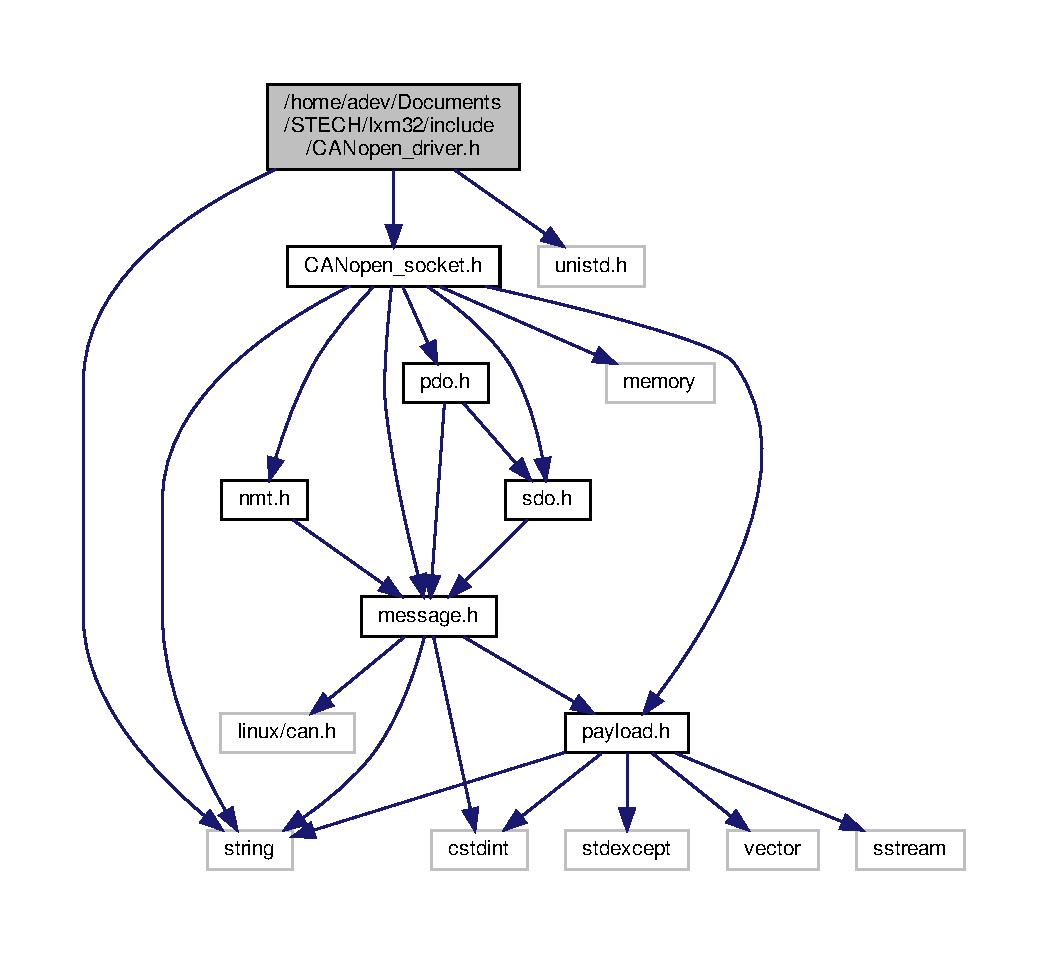
\includegraphics[width=350pt]{_c_a_nopen__driver_8h__incl}
\end{center}
\end{figure}
This graph shows which files directly or indirectly include this file\+:\nopagebreak
\begin{figure}[H]
\begin{center}
\leavevmode
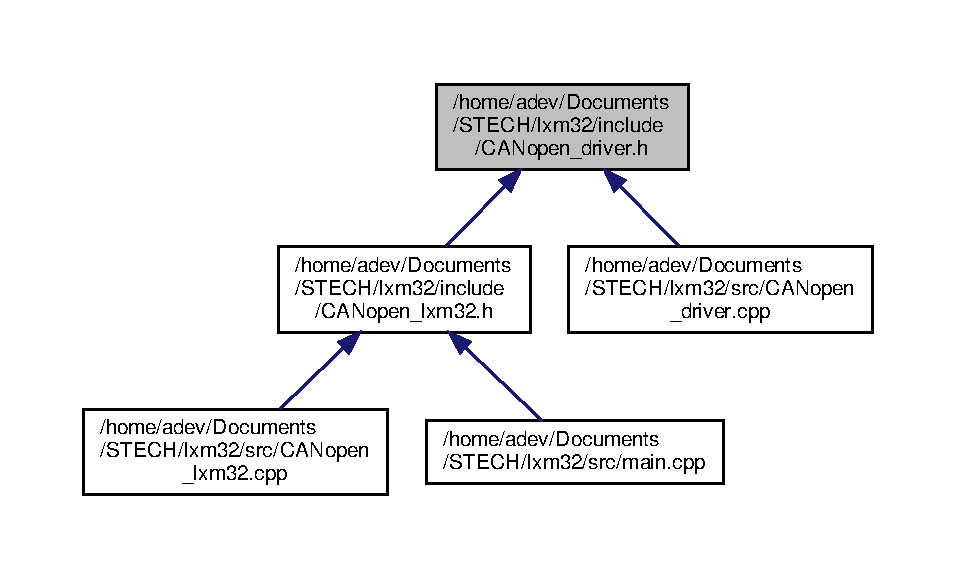
\includegraphics[width=350pt]{_c_a_nopen__driver_8h__dep__incl}
\end{center}
\end{figure}
\subsection*{Classes}
\begin{DoxyCompactItemize}
\item 
class \hyperlink{class_c_a_nopen_1_1_driver}{C\+A\+Nopen\+::\+Driver}
\end{DoxyCompactItemize}
\subsection*{Namespaces}
\begin{DoxyCompactItemize}
\item 
 \hyperlink{namespace_c_a_nopen}{C\+A\+Nopen}
\end{DoxyCompactItemize}
\subsection*{Macros}
\begin{DoxyCompactItemize}
\item 
\#define \hyperlink{_c_a_nopen__driver_8h_a288301cb406c37bce2e676a61a47069f}{R\+E\+G\+\_\+\+C\+A\+Naddress}~0x30410002
\item 
\#define \hyperlink{_c_a_nopen__driver_8h_a0cc1502471745a5a5d2953588405e4bb}{R\+E\+G\+\_\+\+C\+A\+Nbaud}~0x30410003
\item 
\#define \hyperlink{_c_a_nopen__driver_8h_a45fd1c3357c3e7820e73914b4aa2d3ee}{R\+E\+G\+\_\+\+\_\+\+D\+C\+O\+Mstatus}~0x60410000
\item 
\#define \hyperlink{_c_a_nopen__driver_8h_adb964aa4eaba974ed438fee7b9d09ccd}{R\+E\+G\+\_\+\+D\+C\+O\+Mopmode}~0x60600000
\item 
\#define \hyperlink{_c_a_nopen__driver_8h_a37233bac366559f38558d6ffeb5daf01}{R\+E\+G\+\_\+\+D\+C\+O\+Mcontrol}~0x60400000
\item 
\#define \hyperlink{_c_a_nopen__driver_8h_ac2ea552341a2aacf207cfc8c8bcc27af}{R\+E\+G\+\_\+\+P\+Pp\+\_\+target}~0x607\+A0000
\item 
\#define \hyperlink{_c_a_nopen__driver_8h_a5684fffd76d166871a0f7618cb33fa76}{R\+E\+G\+\_\+\+P\+Pv\+\_\+target}~0x60810000
\item 
\#define \hyperlink{_c_a_nopen__driver_8h_a07c414261b71522cb583f0d3c7ab6438}{R\+E\+G\+\_\+\+R\+A\+M\+P\+\_\+v\+\_\+acc}~0x60830000
\item 
\#define \hyperlink{_c_a_nopen__driver_8h_a4e601755eeb2edadf1501afef2bfe234}{R\+E\+G\+\_\+\+R\+A\+M\+P\+\_\+v\+\_\+dec}~0x60840000
\item 
\#define \hyperlink{_c_a_nopen__driver_8h_aac1fb3a95430fb03df0455a3e849d076}{R\+E\+G\+\_\+\+P\+Poption}~0x60\+F20000
\item 
\#define \hyperlink{_c_a_nopen__driver_8h_ab2aeca9392d3d3fe2889e2a4799e53a4}{R\+E\+G\+\_\+\+J\+O\+Gactivate}~0x301\+B0009
\item 
\#define \hyperlink{_c_a_nopen__driver_8h_abd03ed23facc5aa2eac935fa69608547}{M\+O\+D\+E\+\_\+\+Profile\+Position}~1
\item 
\#define \hyperlink{_c_a_nopen__driver_8h_a73172a8fb87a3183ff29444335ba4fdb}{P\+Pctrl\+\_\+\+S\+E\+T\+\_\+\+P\+O\+I\+NT}~0x0010
\item 
\#define \hyperlink{_c_a_nopen__driver_8h_a88648c72edc2879a93ba4723ae3652e7}{P\+Pctrl\+\_\+\+O\+N\+\_\+\+T\+A\+R\+G\+ET}~0x0040
\item 
\#define \hyperlink{_c_a_nopen__driver_8h_ab9cafb4211b0fa97cfc73b15d7b72b11}{P\+Pctrl\+\_\+\+O\+N\+\_\+\+D\+I\+R\+E\+CT}~0x0020
\item 
\#define \hyperlink{_c_a_nopen__driver_8h_a0349d409f0d302bb5374bcd5cd77c126}{P\+Pctrl\+\_\+\+R\+E\+L\+A\+T\+I\+VE}~0x0040
\item 
\#define \hyperlink{_c_a_nopen__driver_8h_ac8368603aa9e8065efb0a231bd007ee5}{P\+Pctrl\+\_\+\+A\+B\+S\+O\+L\+U\+TE}~0x0000
\item 
\#define \hyperlink{_c_a_nopen__driver_8h_ac4772c1c1c24a4b5837a2000c62aa0a3}{O\+P\+\_\+\+S\+H\+U\+T\+D\+O\+WN}~0x0006
\item 
\#define \hyperlink{_c_a_nopen__driver_8h_acf9b640777e01c586865a1b2791fc8b9}{O\+P\+\_\+\+S\+W\+I\+T\+C\+H\+ON}~0x0007
\item 
\#define \hyperlink{_c_a_nopen__driver_8h_a05d94d73527d10913d800850b4ea65f4}{O\+P\+\_\+\+D\+I\+S\+A\+B\+L\+E\+V\+OL}~0x0000
\item 
\#define \hyperlink{_c_a_nopen__driver_8h_ac3cecf02598899083372e24e0093544c}{O\+P\+\_\+\+Q\+U\+I\+C\+K\+S\+T\+OP}~0x0002
\item 
\#define \hyperlink{_c_a_nopen__driver_8h_ad45ed0f1fc61ec91eea44c1e64daac17}{O\+P\+\_\+\+D\+I\+S\+A\+B\+L\+E\+OP}~0x0007
\item 
\#define \hyperlink{_c_a_nopen__driver_8h_ac2d32ebfb52f2cf10d7fec601f266a0f}{O\+P\+\_\+\+E\+N\+A\+B\+L\+E\+OP}~0x000F
\item 
\#define \hyperlink{_c_a_nopen__driver_8h_a64e5209a86a8aa06bd3e71c354616b1c}{O\+P\+\_\+\+F\+A\+U\+L\+T\+R\+E\+S\+E\+ST}~0x0080
\end{DoxyCompactItemize}


\subsection{Macro Definition Documentation}
\mbox{\Hypertarget{_c_a_nopen__driver_8h_abd03ed23facc5aa2eac935fa69608547}\label{_c_a_nopen__driver_8h_abd03ed23facc5aa2eac935fa69608547}} 
\index{C\+A\+Nopen\+\_\+driver.\+h@{C\+A\+Nopen\+\_\+driver.\+h}!M\+O\+D\+E\+\_\+\+Profile\+Position@{M\+O\+D\+E\+\_\+\+Profile\+Position}}
\index{M\+O\+D\+E\+\_\+\+Profile\+Position@{M\+O\+D\+E\+\_\+\+Profile\+Position}!C\+A\+Nopen\+\_\+driver.\+h@{C\+A\+Nopen\+\_\+driver.\+h}}
\subsubsection{\texorpdfstring{M\+O\+D\+E\+\_\+\+Profile\+Position}{MODE\_ProfilePosition}}
{\footnotesize\ttfamily \#define M\+O\+D\+E\+\_\+\+Profile\+Position~1}



Definition at line 25 of file C\+A\+Nopen\+\_\+driver.\+h.

\mbox{\Hypertarget{_c_a_nopen__driver_8h_ad45ed0f1fc61ec91eea44c1e64daac17}\label{_c_a_nopen__driver_8h_ad45ed0f1fc61ec91eea44c1e64daac17}} 
\index{C\+A\+Nopen\+\_\+driver.\+h@{C\+A\+Nopen\+\_\+driver.\+h}!O\+P\+\_\+\+D\+I\+S\+A\+B\+L\+E\+OP@{O\+P\+\_\+\+D\+I\+S\+A\+B\+L\+E\+OP}}
\index{O\+P\+\_\+\+D\+I\+S\+A\+B\+L\+E\+OP@{O\+P\+\_\+\+D\+I\+S\+A\+B\+L\+E\+OP}!C\+A\+Nopen\+\_\+driver.\+h@{C\+A\+Nopen\+\_\+driver.\+h}}
\subsubsection{\texorpdfstring{O\+P\+\_\+\+D\+I\+S\+A\+B\+L\+E\+OP}{OP\_DISABLEOP}}
{\footnotesize\ttfamily \#define O\+P\+\_\+\+D\+I\+S\+A\+B\+L\+E\+OP~0x0007}



Definition at line 36 of file C\+A\+Nopen\+\_\+driver.\+h.

\mbox{\Hypertarget{_c_a_nopen__driver_8h_a05d94d73527d10913d800850b4ea65f4}\label{_c_a_nopen__driver_8h_a05d94d73527d10913d800850b4ea65f4}} 
\index{C\+A\+Nopen\+\_\+driver.\+h@{C\+A\+Nopen\+\_\+driver.\+h}!O\+P\+\_\+\+D\+I\+S\+A\+B\+L\+E\+V\+OL@{O\+P\+\_\+\+D\+I\+S\+A\+B\+L\+E\+V\+OL}}
\index{O\+P\+\_\+\+D\+I\+S\+A\+B\+L\+E\+V\+OL@{O\+P\+\_\+\+D\+I\+S\+A\+B\+L\+E\+V\+OL}!C\+A\+Nopen\+\_\+driver.\+h@{C\+A\+Nopen\+\_\+driver.\+h}}
\subsubsection{\texorpdfstring{O\+P\+\_\+\+D\+I\+S\+A\+B\+L\+E\+V\+OL}{OP\_DISABLEVOL}}
{\footnotesize\ttfamily \#define O\+P\+\_\+\+D\+I\+S\+A\+B\+L\+E\+V\+OL~0x0000}



Definition at line 34 of file C\+A\+Nopen\+\_\+driver.\+h.

\mbox{\Hypertarget{_c_a_nopen__driver_8h_ac2d32ebfb52f2cf10d7fec601f266a0f}\label{_c_a_nopen__driver_8h_ac2d32ebfb52f2cf10d7fec601f266a0f}} 
\index{C\+A\+Nopen\+\_\+driver.\+h@{C\+A\+Nopen\+\_\+driver.\+h}!O\+P\+\_\+\+E\+N\+A\+B\+L\+E\+OP@{O\+P\+\_\+\+E\+N\+A\+B\+L\+E\+OP}}
\index{O\+P\+\_\+\+E\+N\+A\+B\+L\+E\+OP@{O\+P\+\_\+\+E\+N\+A\+B\+L\+E\+OP}!C\+A\+Nopen\+\_\+driver.\+h@{C\+A\+Nopen\+\_\+driver.\+h}}
\subsubsection{\texorpdfstring{O\+P\+\_\+\+E\+N\+A\+B\+L\+E\+OP}{OP\_ENABLEOP}}
{\footnotesize\ttfamily \#define O\+P\+\_\+\+E\+N\+A\+B\+L\+E\+OP~0x000F}



Definition at line 37 of file C\+A\+Nopen\+\_\+driver.\+h.

\mbox{\Hypertarget{_c_a_nopen__driver_8h_a64e5209a86a8aa06bd3e71c354616b1c}\label{_c_a_nopen__driver_8h_a64e5209a86a8aa06bd3e71c354616b1c}} 
\index{C\+A\+Nopen\+\_\+driver.\+h@{C\+A\+Nopen\+\_\+driver.\+h}!O\+P\+\_\+\+F\+A\+U\+L\+T\+R\+E\+S\+E\+ST@{O\+P\+\_\+\+F\+A\+U\+L\+T\+R\+E\+S\+E\+ST}}
\index{O\+P\+\_\+\+F\+A\+U\+L\+T\+R\+E\+S\+E\+ST@{O\+P\+\_\+\+F\+A\+U\+L\+T\+R\+E\+S\+E\+ST}!C\+A\+Nopen\+\_\+driver.\+h@{C\+A\+Nopen\+\_\+driver.\+h}}
\subsubsection{\texorpdfstring{O\+P\+\_\+\+F\+A\+U\+L\+T\+R\+E\+S\+E\+ST}{OP\_FAULTRESEST}}
{\footnotesize\ttfamily \#define O\+P\+\_\+\+F\+A\+U\+L\+T\+R\+E\+S\+E\+ST~0x0080}



Definition at line 38 of file C\+A\+Nopen\+\_\+driver.\+h.

\mbox{\Hypertarget{_c_a_nopen__driver_8h_ac3cecf02598899083372e24e0093544c}\label{_c_a_nopen__driver_8h_ac3cecf02598899083372e24e0093544c}} 
\index{C\+A\+Nopen\+\_\+driver.\+h@{C\+A\+Nopen\+\_\+driver.\+h}!O\+P\+\_\+\+Q\+U\+I\+C\+K\+S\+T\+OP@{O\+P\+\_\+\+Q\+U\+I\+C\+K\+S\+T\+OP}}
\index{O\+P\+\_\+\+Q\+U\+I\+C\+K\+S\+T\+OP@{O\+P\+\_\+\+Q\+U\+I\+C\+K\+S\+T\+OP}!C\+A\+Nopen\+\_\+driver.\+h@{C\+A\+Nopen\+\_\+driver.\+h}}
\subsubsection{\texorpdfstring{O\+P\+\_\+\+Q\+U\+I\+C\+K\+S\+T\+OP}{OP\_QUICKSTOP}}
{\footnotesize\ttfamily \#define O\+P\+\_\+\+Q\+U\+I\+C\+K\+S\+T\+OP~0x0002}



Definition at line 35 of file C\+A\+Nopen\+\_\+driver.\+h.

\mbox{\Hypertarget{_c_a_nopen__driver_8h_ac4772c1c1c24a4b5837a2000c62aa0a3}\label{_c_a_nopen__driver_8h_ac4772c1c1c24a4b5837a2000c62aa0a3}} 
\index{C\+A\+Nopen\+\_\+driver.\+h@{C\+A\+Nopen\+\_\+driver.\+h}!O\+P\+\_\+\+S\+H\+U\+T\+D\+O\+WN@{O\+P\+\_\+\+S\+H\+U\+T\+D\+O\+WN}}
\index{O\+P\+\_\+\+S\+H\+U\+T\+D\+O\+WN@{O\+P\+\_\+\+S\+H\+U\+T\+D\+O\+WN}!C\+A\+Nopen\+\_\+driver.\+h@{C\+A\+Nopen\+\_\+driver.\+h}}
\subsubsection{\texorpdfstring{O\+P\+\_\+\+S\+H\+U\+T\+D\+O\+WN}{OP\_SHUTDOWN}}
{\footnotesize\ttfamily \#define O\+P\+\_\+\+S\+H\+U\+T\+D\+O\+WN~0x0006}



Definition at line 32 of file C\+A\+Nopen\+\_\+driver.\+h.

\mbox{\Hypertarget{_c_a_nopen__driver_8h_acf9b640777e01c586865a1b2791fc8b9}\label{_c_a_nopen__driver_8h_acf9b640777e01c586865a1b2791fc8b9}} 
\index{C\+A\+Nopen\+\_\+driver.\+h@{C\+A\+Nopen\+\_\+driver.\+h}!O\+P\+\_\+\+S\+W\+I\+T\+C\+H\+ON@{O\+P\+\_\+\+S\+W\+I\+T\+C\+H\+ON}}
\index{O\+P\+\_\+\+S\+W\+I\+T\+C\+H\+ON@{O\+P\+\_\+\+S\+W\+I\+T\+C\+H\+ON}!C\+A\+Nopen\+\_\+driver.\+h@{C\+A\+Nopen\+\_\+driver.\+h}}
\subsubsection{\texorpdfstring{O\+P\+\_\+\+S\+W\+I\+T\+C\+H\+ON}{OP\_SWITCHON}}
{\footnotesize\ttfamily \#define O\+P\+\_\+\+S\+W\+I\+T\+C\+H\+ON~0x0007}



Definition at line 33 of file C\+A\+Nopen\+\_\+driver.\+h.

\mbox{\Hypertarget{_c_a_nopen__driver_8h_ac8368603aa9e8065efb0a231bd007ee5}\label{_c_a_nopen__driver_8h_ac8368603aa9e8065efb0a231bd007ee5}} 
\index{C\+A\+Nopen\+\_\+driver.\+h@{C\+A\+Nopen\+\_\+driver.\+h}!P\+Pctrl\+\_\+\+A\+B\+S\+O\+L\+U\+TE@{P\+Pctrl\+\_\+\+A\+B\+S\+O\+L\+U\+TE}}
\index{P\+Pctrl\+\_\+\+A\+B\+S\+O\+L\+U\+TE@{P\+Pctrl\+\_\+\+A\+B\+S\+O\+L\+U\+TE}!C\+A\+Nopen\+\_\+driver.\+h@{C\+A\+Nopen\+\_\+driver.\+h}}
\subsubsection{\texorpdfstring{P\+Pctrl\+\_\+\+A\+B\+S\+O\+L\+U\+TE}{PPctrl\_ABSOLUTE}}
{\footnotesize\ttfamily \#define P\+Pctrl\+\_\+\+A\+B\+S\+O\+L\+U\+TE~0x0000}



Definition at line 30 of file C\+A\+Nopen\+\_\+driver.\+h.

\mbox{\Hypertarget{_c_a_nopen__driver_8h_ab9cafb4211b0fa97cfc73b15d7b72b11}\label{_c_a_nopen__driver_8h_ab9cafb4211b0fa97cfc73b15d7b72b11}} 
\index{C\+A\+Nopen\+\_\+driver.\+h@{C\+A\+Nopen\+\_\+driver.\+h}!P\+Pctrl\+\_\+\+O\+N\+\_\+\+D\+I\+R\+E\+CT@{P\+Pctrl\+\_\+\+O\+N\+\_\+\+D\+I\+R\+E\+CT}}
\index{P\+Pctrl\+\_\+\+O\+N\+\_\+\+D\+I\+R\+E\+CT@{P\+Pctrl\+\_\+\+O\+N\+\_\+\+D\+I\+R\+E\+CT}!C\+A\+Nopen\+\_\+driver.\+h@{C\+A\+Nopen\+\_\+driver.\+h}}
\subsubsection{\texorpdfstring{P\+Pctrl\+\_\+\+O\+N\+\_\+\+D\+I\+R\+E\+CT}{PPctrl\_ON\_DIRECT}}
{\footnotesize\ttfamily \#define P\+Pctrl\+\_\+\+O\+N\+\_\+\+D\+I\+R\+E\+CT~0x0020}



Definition at line 28 of file C\+A\+Nopen\+\_\+driver.\+h.

\mbox{\Hypertarget{_c_a_nopen__driver_8h_a88648c72edc2879a93ba4723ae3652e7}\label{_c_a_nopen__driver_8h_a88648c72edc2879a93ba4723ae3652e7}} 
\index{C\+A\+Nopen\+\_\+driver.\+h@{C\+A\+Nopen\+\_\+driver.\+h}!P\+Pctrl\+\_\+\+O\+N\+\_\+\+T\+A\+R\+G\+ET@{P\+Pctrl\+\_\+\+O\+N\+\_\+\+T\+A\+R\+G\+ET}}
\index{P\+Pctrl\+\_\+\+O\+N\+\_\+\+T\+A\+R\+G\+ET@{P\+Pctrl\+\_\+\+O\+N\+\_\+\+T\+A\+R\+G\+ET}!C\+A\+Nopen\+\_\+driver.\+h@{C\+A\+Nopen\+\_\+driver.\+h}}
\subsubsection{\texorpdfstring{P\+Pctrl\+\_\+\+O\+N\+\_\+\+T\+A\+R\+G\+ET}{PPctrl\_ON\_TARGET}}
{\footnotesize\ttfamily \#define P\+Pctrl\+\_\+\+O\+N\+\_\+\+T\+A\+R\+G\+ET~0x0040}



Definition at line 27 of file C\+A\+Nopen\+\_\+driver.\+h.

\mbox{\Hypertarget{_c_a_nopen__driver_8h_a0349d409f0d302bb5374bcd5cd77c126}\label{_c_a_nopen__driver_8h_a0349d409f0d302bb5374bcd5cd77c126}} 
\index{C\+A\+Nopen\+\_\+driver.\+h@{C\+A\+Nopen\+\_\+driver.\+h}!P\+Pctrl\+\_\+\+R\+E\+L\+A\+T\+I\+VE@{P\+Pctrl\+\_\+\+R\+E\+L\+A\+T\+I\+VE}}
\index{P\+Pctrl\+\_\+\+R\+E\+L\+A\+T\+I\+VE@{P\+Pctrl\+\_\+\+R\+E\+L\+A\+T\+I\+VE}!C\+A\+Nopen\+\_\+driver.\+h@{C\+A\+Nopen\+\_\+driver.\+h}}
\subsubsection{\texorpdfstring{P\+Pctrl\+\_\+\+R\+E\+L\+A\+T\+I\+VE}{PPctrl\_RELATIVE}}
{\footnotesize\ttfamily \#define P\+Pctrl\+\_\+\+R\+E\+L\+A\+T\+I\+VE~0x0040}



Definition at line 29 of file C\+A\+Nopen\+\_\+driver.\+h.

\mbox{\Hypertarget{_c_a_nopen__driver_8h_a73172a8fb87a3183ff29444335ba4fdb}\label{_c_a_nopen__driver_8h_a73172a8fb87a3183ff29444335ba4fdb}} 
\index{C\+A\+Nopen\+\_\+driver.\+h@{C\+A\+Nopen\+\_\+driver.\+h}!P\+Pctrl\+\_\+\+S\+E\+T\+\_\+\+P\+O\+I\+NT@{P\+Pctrl\+\_\+\+S\+E\+T\+\_\+\+P\+O\+I\+NT}}
\index{P\+Pctrl\+\_\+\+S\+E\+T\+\_\+\+P\+O\+I\+NT@{P\+Pctrl\+\_\+\+S\+E\+T\+\_\+\+P\+O\+I\+NT}!C\+A\+Nopen\+\_\+driver.\+h@{C\+A\+Nopen\+\_\+driver.\+h}}
\subsubsection{\texorpdfstring{P\+Pctrl\+\_\+\+S\+E\+T\+\_\+\+P\+O\+I\+NT}{PPctrl\_SET\_POINT}}
{\footnotesize\ttfamily \#define P\+Pctrl\+\_\+\+S\+E\+T\+\_\+\+P\+O\+I\+NT~0x0010}



Definition at line 26 of file C\+A\+Nopen\+\_\+driver.\+h.

\mbox{\Hypertarget{_c_a_nopen__driver_8h_a45fd1c3357c3e7820e73914b4aa2d3ee}\label{_c_a_nopen__driver_8h_a45fd1c3357c3e7820e73914b4aa2d3ee}} 
\index{C\+A\+Nopen\+\_\+driver.\+h@{C\+A\+Nopen\+\_\+driver.\+h}!R\+E\+G\+\_\+\+\_\+\+D\+C\+O\+Mstatus@{R\+E\+G\+\_\+\+\_\+\+D\+C\+O\+Mstatus}}
\index{R\+E\+G\+\_\+\+\_\+\+D\+C\+O\+Mstatus@{R\+E\+G\+\_\+\+\_\+\+D\+C\+O\+Mstatus}!C\+A\+Nopen\+\_\+driver.\+h@{C\+A\+Nopen\+\_\+driver.\+h}}
\subsubsection{\texorpdfstring{R\+E\+G\+\_\+\+\_\+\+D\+C\+O\+Mstatus}{REG\_\_DCOMstatus}}
{\footnotesize\ttfamily \#define R\+E\+G\+\_\+\+\_\+\+D\+C\+O\+Mstatus~0x60410000}



Definition at line 12 of file C\+A\+Nopen\+\_\+driver.\+h.

\mbox{\Hypertarget{_c_a_nopen__driver_8h_a288301cb406c37bce2e676a61a47069f}\label{_c_a_nopen__driver_8h_a288301cb406c37bce2e676a61a47069f}} 
\index{C\+A\+Nopen\+\_\+driver.\+h@{C\+A\+Nopen\+\_\+driver.\+h}!R\+E\+G\+\_\+\+C\+A\+Naddress@{R\+E\+G\+\_\+\+C\+A\+Naddress}}
\index{R\+E\+G\+\_\+\+C\+A\+Naddress@{R\+E\+G\+\_\+\+C\+A\+Naddress}!C\+A\+Nopen\+\_\+driver.\+h@{C\+A\+Nopen\+\_\+driver.\+h}}
\subsubsection{\texorpdfstring{R\+E\+G\+\_\+\+C\+A\+Naddress}{REG\_CANaddress}}
{\footnotesize\ttfamily \#define R\+E\+G\+\_\+\+C\+A\+Naddress~0x30410002}



Definition at line 9 of file C\+A\+Nopen\+\_\+driver.\+h.

\mbox{\Hypertarget{_c_a_nopen__driver_8h_a0cc1502471745a5a5d2953588405e4bb}\label{_c_a_nopen__driver_8h_a0cc1502471745a5a5d2953588405e4bb}} 
\index{C\+A\+Nopen\+\_\+driver.\+h@{C\+A\+Nopen\+\_\+driver.\+h}!R\+E\+G\+\_\+\+C\+A\+Nbaud@{R\+E\+G\+\_\+\+C\+A\+Nbaud}}
\index{R\+E\+G\+\_\+\+C\+A\+Nbaud@{R\+E\+G\+\_\+\+C\+A\+Nbaud}!C\+A\+Nopen\+\_\+driver.\+h@{C\+A\+Nopen\+\_\+driver.\+h}}
\subsubsection{\texorpdfstring{R\+E\+G\+\_\+\+C\+A\+Nbaud}{REG\_CANbaud}}
{\footnotesize\ttfamily \#define R\+E\+G\+\_\+\+C\+A\+Nbaud~0x30410003}



Definition at line 10 of file C\+A\+Nopen\+\_\+driver.\+h.

\mbox{\Hypertarget{_c_a_nopen__driver_8h_a37233bac366559f38558d6ffeb5daf01}\label{_c_a_nopen__driver_8h_a37233bac366559f38558d6ffeb5daf01}} 
\index{C\+A\+Nopen\+\_\+driver.\+h@{C\+A\+Nopen\+\_\+driver.\+h}!R\+E\+G\+\_\+\+D\+C\+O\+Mcontrol@{R\+E\+G\+\_\+\+D\+C\+O\+Mcontrol}}
\index{R\+E\+G\+\_\+\+D\+C\+O\+Mcontrol@{R\+E\+G\+\_\+\+D\+C\+O\+Mcontrol}!C\+A\+Nopen\+\_\+driver.\+h@{C\+A\+Nopen\+\_\+driver.\+h}}
\subsubsection{\texorpdfstring{R\+E\+G\+\_\+\+D\+C\+O\+Mcontrol}{REG\_DCOMcontrol}}
{\footnotesize\ttfamily \#define R\+E\+G\+\_\+\+D\+C\+O\+Mcontrol~0x60400000}



Definition at line 14 of file C\+A\+Nopen\+\_\+driver.\+h.

\mbox{\Hypertarget{_c_a_nopen__driver_8h_adb964aa4eaba974ed438fee7b9d09ccd}\label{_c_a_nopen__driver_8h_adb964aa4eaba974ed438fee7b9d09ccd}} 
\index{C\+A\+Nopen\+\_\+driver.\+h@{C\+A\+Nopen\+\_\+driver.\+h}!R\+E\+G\+\_\+\+D\+C\+O\+Mopmode@{R\+E\+G\+\_\+\+D\+C\+O\+Mopmode}}
\index{R\+E\+G\+\_\+\+D\+C\+O\+Mopmode@{R\+E\+G\+\_\+\+D\+C\+O\+Mopmode}!C\+A\+Nopen\+\_\+driver.\+h@{C\+A\+Nopen\+\_\+driver.\+h}}
\subsubsection{\texorpdfstring{R\+E\+G\+\_\+\+D\+C\+O\+Mopmode}{REG\_DCOMopmode}}
{\footnotesize\ttfamily \#define R\+E\+G\+\_\+\+D\+C\+O\+Mopmode~0x60600000}



Definition at line 13 of file C\+A\+Nopen\+\_\+driver.\+h.

\mbox{\Hypertarget{_c_a_nopen__driver_8h_ab2aeca9392d3d3fe2889e2a4799e53a4}\label{_c_a_nopen__driver_8h_ab2aeca9392d3d3fe2889e2a4799e53a4}} 
\index{C\+A\+Nopen\+\_\+driver.\+h@{C\+A\+Nopen\+\_\+driver.\+h}!R\+E\+G\+\_\+\+J\+O\+Gactivate@{R\+E\+G\+\_\+\+J\+O\+Gactivate}}
\index{R\+E\+G\+\_\+\+J\+O\+Gactivate@{R\+E\+G\+\_\+\+J\+O\+Gactivate}!C\+A\+Nopen\+\_\+driver.\+h@{C\+A\+Nopen\+\_\+driver.\+h}}
\subsubsection{\texorpdfstring{R\+E\+G\+\_\+\+J\+O\+Gactivate}{REG\_JOGactivate}}
{\footnotesize\ttfamily \#define R\+E\+G\+\_\+\+J\+O\+Gactivate~0x301\+B0009}



Definition at line 23 of file C\+A\+Nopen\+\_\+driver.\+h.

\mbox{\Hypertarget{_c_a_nopen__driver_8h_aac1fb3a95430fb03df0455a3e849d076}\label{_c_a_nopen__driver_8h_aac1fb3a95430fb03df0455a3e849d076}} 
\index{C\+A\+Nopen\+\_\+driver.\+h@{C\+A\+Nopen\+\_\+driver.\+h}!R\+E\+G\+\_\+\+P\+Poption@{R\+E\+G\+\_\+\+P\+Poption}}
\index{R\+E\+G\+\_\+\+P\+Poption@{R\+E\+G\+\_\+\+P\+Poption}!C\+A\+Nopen\+\_\+driver.\+h@{C\+A\+Nopen\+\_\+driver.\+h}}
\subsubsection{\texorpdfstring{R\+E\+G\+\_\+\+P\+Poption}{REG\_PPoption}}
{\footnotesize\ttfamily \#define R\+E\+G\+\_\+\+P\+Poption~0x60\+F20000}



Definition at line 21 of file C\+A\+Nopen\+\_\+driver.\+h.

\mbox{\Hypertarget{_c_a_nopen__driver_8h_ac2ea552341a2aacf207cfc8c8bcc27af}\label{_c_a_nopen__driver_8h_ac2ea552341a2aacf207cfc8c8bcc27af}} 
\index{C\+A\+Nopen\+\_\+driver.\+h@{C\+A\+Nopen\+\_\+driver.\+h}!R\+E\+G\+\_\+\+P\+Pp\+\_\+target@{R\+E\+G\+\_\+\+P\+Pp\+\_\+target}}
\index{R\+E\+G\+\_\+\+P\+Pp\+\_\+target@{R\+E\+G\+\_\+\+P\+Pp\+\_\+target}!C\+A\+Nopen\+\_\+driver.\+h@{C\+A\+Nopen\+\_\+driver.\+h}}
\subsubsection{\texorpdfstring{R\+E\+G\+\_\+\+P\+Pp\+\_\+target}{REG\_PPp\_target}}
{\footnotesize\ttfamily \#define R\+E\+G\+\_\+\+P\+Pp\+\_\+target~0x607\+A0000}



Definition at line 16 of file C\+A\+Nopen\+\_\+driver.\+h.

\mbox{\Hypertarget{_c_a_nopen__driver_8h_a5684fffd76d166871a0f7618cb33fa76}\label{_c_a_nopen__driver_8h_a5684fffd76d166871a0f7618cb33fa76}} 
\index{C\+A\+Nopen\+\_\+driver.\+h@{C\+A\+Nopen\+\_\+driver.\+h}!R\+E\+G\+\_\+\+P\+Pv\+\_\+target@{R\+E\+G\+\_\+\+P\+Pv\+\_\+target}}
\index{R\+E\+G\+\_\+\+P\+Pv\+\_\+target@{R\+E\+G\+\_\+\+P\+Pv\+\_\+target}!C\+A\+Nopen\+\_\+driver.\+h@{C\+A\+Nopen\+\_\+driver.\+h}}
\subsubsection{\texorpdfstring{R\+E\+G\+\_\+\+P\+Pv\+\_\+target}{REG\_PPv\_target}}
{\footnotesize\ttfamily \#define R\+E\+G\+\_\+\+P\+Pv\+\_\+target~0x60810000}



Definition at line 17 of file C\+A\+Nopen\+\_\+driver.\+h.

\mbox{\Hypertarget{_c_a_nopen__driver_8h_a07c414261b71522cb583f0d3c7ab6438}\label{_c_a_nopen__driver_8h_a07c414261b71522cb583f0d3c7ab6438}} 
\index{C\+A\+Nopen\+\_\+driver.\+h@{C\+A\+Nopen\+\_\+driver.\+h}!R\+E\+G\+\_\+\+R\+A\+M\+P\+\_\+v\+\_\+acc@{R\+E\+G\+\_\+\+R\+A\+M\+P\+\_\+v\+\_\+acc}}
\index{R\+E\+G\+\_\+\+R\+A\+M\+P\+\_\+v\+\_\+acc@{R\+E\+G\+\_\+\+R\+A\+M\+P\+\_\+v\+\_\+acc}!C\+A\+Nopen\+\_\+driver.\+h@{C\+A\+Nopen\+\_\+driver.\+h}}
\subsubsection{\texorpdfstring{R\+E\+G\+\_\+\+R\+A\+M\+P\+\_\+v\+\_\+acc}{REG\_RAMP\_v\_acc}}
{\footnotesize\ttfamily \#define R\+E\+G\+\_\+\+R\+A\+M\+P\+\_\+v\+\_\+acc~0x60830000}



Definition at line 18 of file C\+A\+Nopen\+\_\+driver.\+h.

\mbox{\Hypertarget{_c_a_nopen__driver_8h_a4e601755eeb2edadf1501afef2bfe234}\label{_c_a_nopen__driver_8h_a4e601755eeb2edadf1501afef2bfe234}} 
\index{C\+A\+Nopen\+\_\+driver.\+h@{C\+A\+Nopen\+\_\+driver.\+h}!R\+E\+G\+\_\+\+R\+A\+M\+P\+\_\+v\+\_\+dec@{R\+E\+G\+\_\+\+R\+A\+M\+P\+\_\+v\+\_\+dec}}
\index{R\+E\+G\+\_\+\+R\+A\+M\+P\+\_\+v\+\_\+dec@{R\+E\+G\+\_\+\+R\+A\+M\+P\+\_\+v\+\_\+dec}!C\+A\+Nopen\+\_\+driver.\+h@{C\+A\+Nopen\+\_\+driver.\+h}}
\subsubsection{\texorpdfstring{R\+E\+G\+\_\+\+R\+A\+M\+P\+\_\+v\+\_\+dec}{REG\_RAMP\_v\_dec}}
{\footnotesize\ttfamily \#define R\+E\+G\+\_\+\+R\+A\+M\+P\+\_\+v\+\_\+dec~0x60840000}



Definition at line 19 of file C\+A\+Nopen\+\_\+driver.\+h.


\hypertarget{_c_a_nopen__lxm32_8h}{}\section{/home/adev/\+Documents/\+S\+T\+E\+C\+H/lxm32/include/\+C\+A\+Nopen\+\_\+lxm32.h File Reference}
\label{_c_a_nopen__lxm32_8h}\index{/home/adev/\+Documents/\+S\+T\+E\+C\+H/lxm32/include/\+C\+A\+Nopen\+\_\+lxm32.\+h@{/home/adev/\+Documents/\+S\+T\+E\+C\+H/lxm32/include/\+C\+A\+Nopen\+\_\+lxm32.\+h}}
{\ttfamily \#include \char`\"{}C\+A\+Nopen\+\_\+driver.\+h\char`\"{}}\newline
{\ttfamily \#include $<$string$>$}\newline
{\ttfamily \#include $<$unistd.\+h$>$}\newline
Include dependency graph for C\+A\+Nopen\+\_\+lxm32.\+h\+:\nopagebreak
\begin{figure}[H]
\begin{center}
\leavevmode
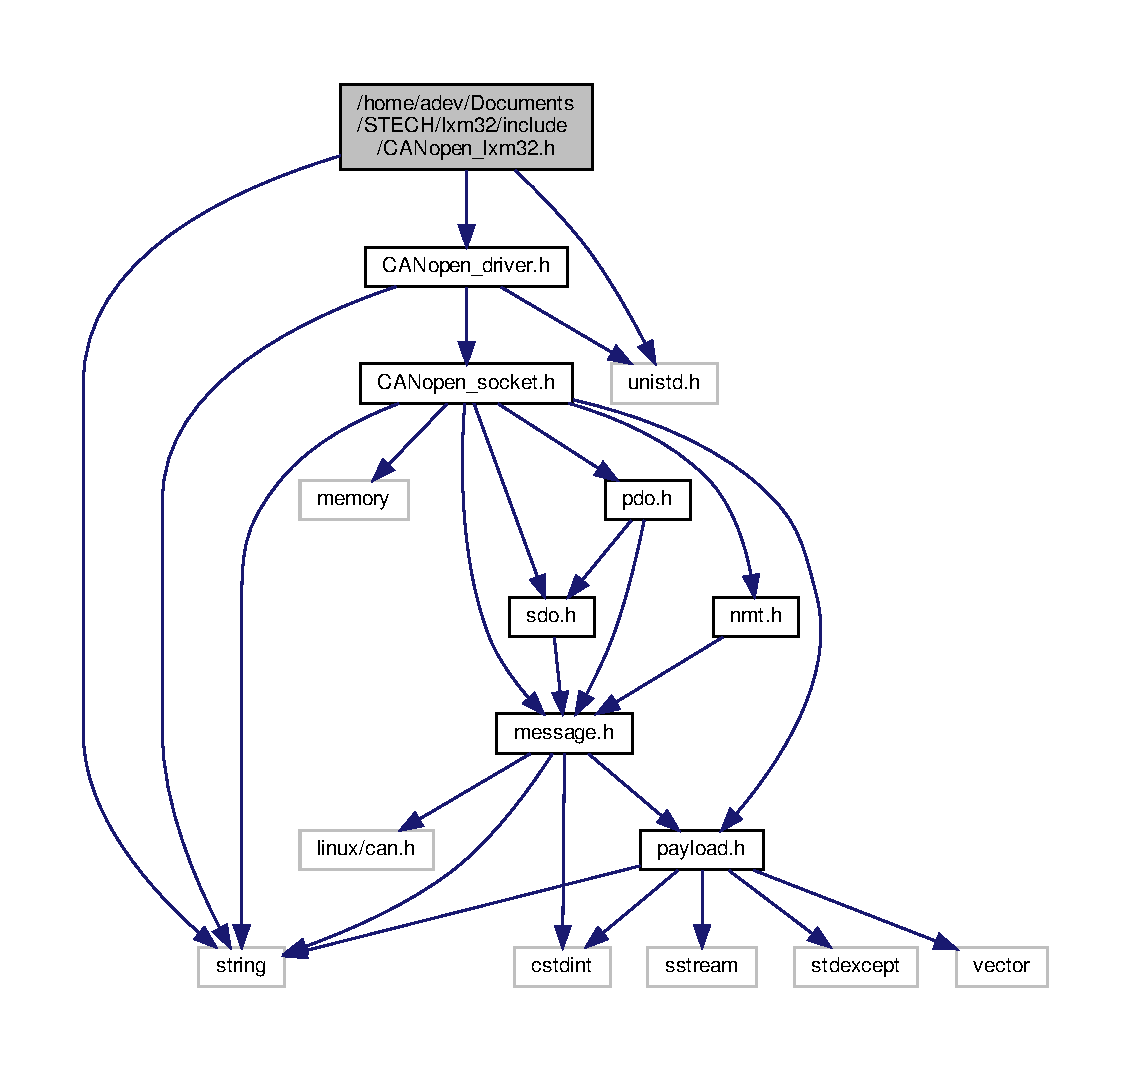
\includegraphics[width=350pt]{_c_a_nopen__lxm32_8h__incl}
\end{center}
\end{figure}
This graph shows which files directly or indirectly include this file\+:\nopagebreak
\begin{figure}[H]
\begin{center}
\leavevmode
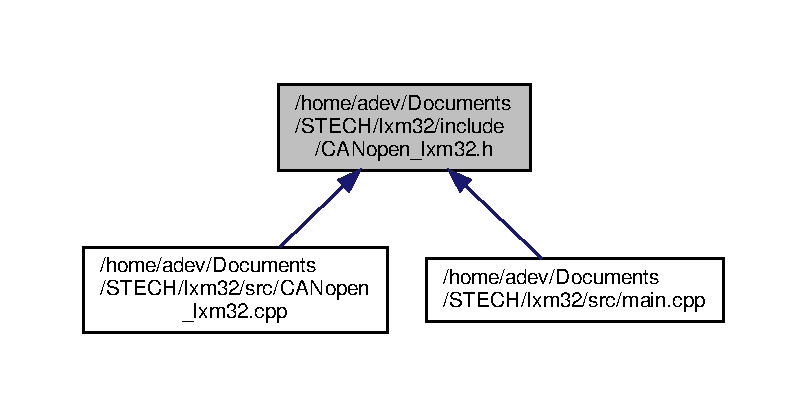
\includegraphics[width=350pt]{_c_a_nopen__lxm32_8h__dep__incl}
\end{center}
\end{figure}
\subsection*{Classes}
\begin{DoxyCompactItemize}
\item 
class \hyperlink{class_c_a_nopen_1_1_l_x_m32}{C\+A\+Nopen\+::\+L\+X\+M32}
\end{DoxyCompactItemize}
\subsection*{Namespaces}
\begin{DoxyCompactItemize}
\item 
 \hyperlink{namespace_c_a_nopen}{C\+A\+Nopen}
\end{DoxyCompactItemize}

\hypertarget{_c_a_nopen__socket_8h}{}\section{/home/adev/\+Documents/\+S\+T\+E\+C\+H/lxm32/lib/canopen/include/\+C\+A\+Nopen\+\_\+socket.h File Reference}
\label{_c_a_nopen__socket_8h}\index{/home/adev/\+Documents/\+S\+T\+E\+C\+H/lxm32/lib/canopen/include/\+C\+A\+Nopen\+\_\+socket.\+h@{/home/adev/\+Documents/\+S\+T\+E\+C\+H/lxm32/lib/canopen/include/\+C\+A\+Nopen\+\_\+socket.\+h}}


Canopen object able to send command through a C\+AN interface using the U\+N\+IX socket.  


{\ttfamily \#include $<$memory$>$}\newline
{\ttfamily \#include $<$string$>$}\newline
{\ttfamily \#include \char`\"{}message.\+h\char`\"{}}\newline
{\ttfamily \#include \char`\"{}payload.\+h\char`\"{}}\newline
{\ttfamily \#include \char`\"{}sdo.\+h\char`\"{}}\newline
{\ttfamily \#include \char`\"{}pdo.\+h\char`\"{}}\newline
{\ttfamily \#include \char`\"{}nmt.\+h\char`\"{}}\newline
Include dependency graph for C\+A\+Nopen\+\_\+socket.\+h\+:\nopagebreak
\begin{figure}[H]
\begin{center}
\leavevmode
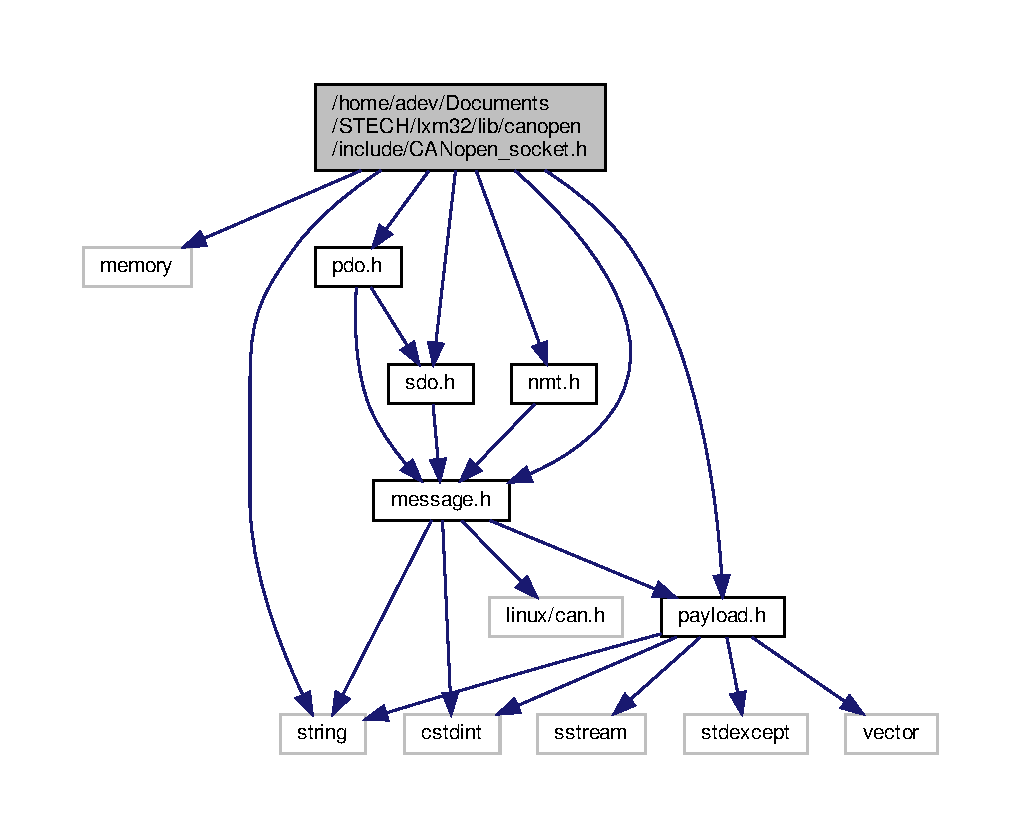
\includegraphics[width=350pt]{_c_a_nopen__socket_8h__incl}
\end{center}
\end{figure}
This graph shows which files directly or indirectly include this file\+:\nopagebreak
\begin{figure}[H]
\begin{center}
\leavevmode
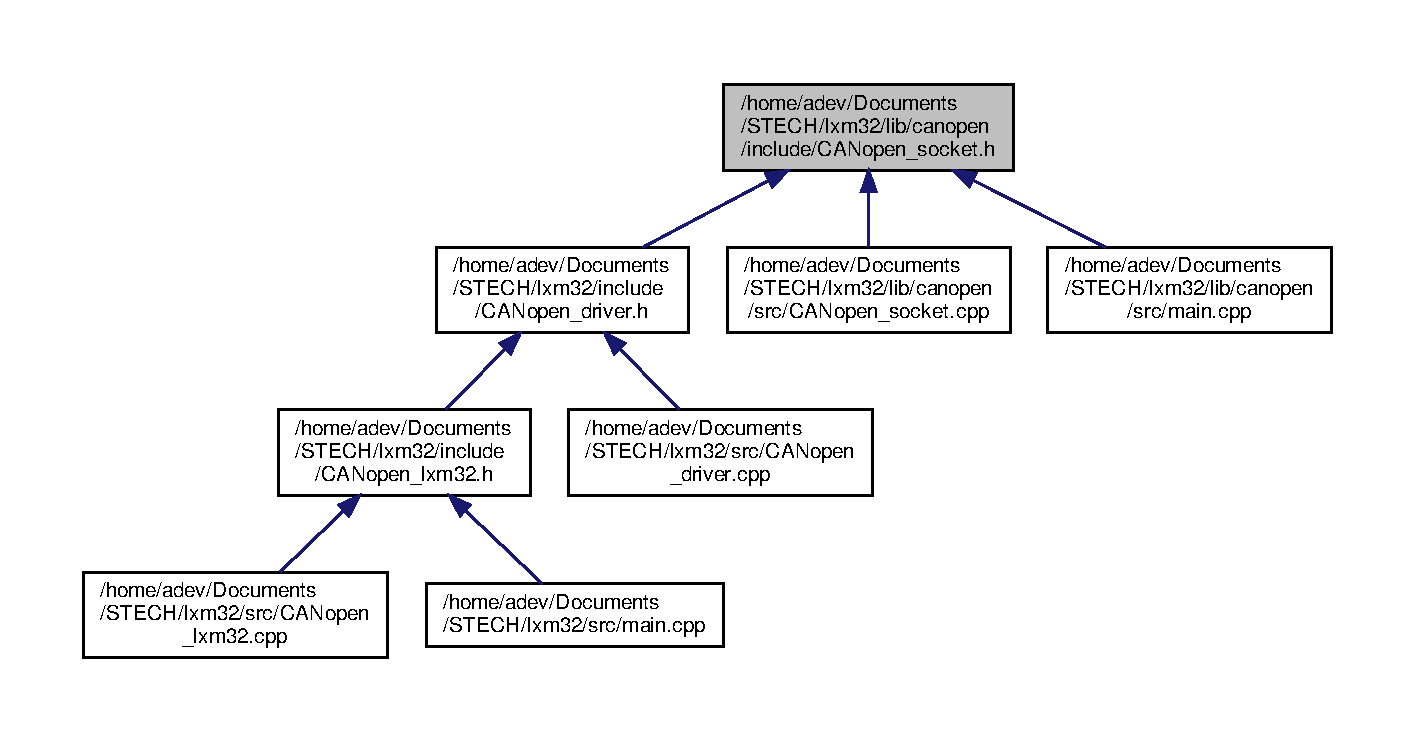
\includegraphics[width=350pt]{_c_a_nopen__socket_8h__dep__incl}
\end{center}
\end{figure}
\subsection*{Classes}
\begin{DoxyCompactItemize}
\item 
class \hyperlink{class_c_a_nopen_1_1_socket}{C\+A\+Nopen\+::\+Socket}
\begin{DoxyCompactList}\small\item\em Canopen object able to send command through a C\+AN interface using U\+N\+IX sockets. \end{DoxyCompactList}\end{DoxyCompactItemize}
\subsection*{Namespaces}
\begin{DoxyCompactItemize}
\item 
 \hyperlink{namespace_c_a_nopen}{C\+A\+Nopen}
\end{DoxyCompactItemize}
\subsection*{Macros}
\begin{DoxyCompactItemize}
\item 
\#define \hyperlink{_c_a_nopen__socket_8h_a86e649743184cb6251a418049d8988f2}{I\+F\+\_\+\+V\+E\+R\+B\+O\+SE}(lvl,  cmd)
\end{DoxyCompactItemize}


\subsection{Detailed Description}
Canopen object able to send command through a C\+AN interface using the U\+N\+IX socket. 

\begin{DoxyAuthor}{Author}
Alexis Devillard 
\end{DoxyAuthor}
\begin{DoxyVersion}{Version}
1.\+0 
\end{DoxyVersion}


\subsection{Macro Definition Documentation}
\mbox{\Hypertarget{_c_a_nopen__socket_8h_a86e649743184cb6251a418049d8988f2}\label{_c_a_nopen__socket_8h_a86e649743184cb6251a418049d8988f2}} 
\index{C\+A\+Nopen\+\_\+socket.\+h@{C\+A\+Nopen\+\_\+socket.\+h}!I\+F\+\_\+\+V\+E\+R\+B\+O\+SE@{I\+F\+\_\+\+V\+E\+R\+B\+O\+SE}}
\index{I\+F\+\_\+\+V\+E\+R\+B\+O\+SE@{I\+F\+\_\+\+V\+E\+R\+B\+O\+SE}!C\+A\+Nopen\+\_\+socket.\+h@{C\+A\+Nopen\+\_\+socket.\+h}}
\subsubsection{\texorpdfstring{I\+F\+\_\+\+V\+E\+R\+B\+O\+SE}{IF\_VERBOSE}}
{\footnotesize\ttfamily \#define I\+F\+\_\+\+V\+E\+R\+B\+O\+SE(\begin{DoxyParamCaption}\item[{}]{lvl,  }\item[{}]{cmd }\end{DoxyParamCaption})}

{\bfseries Value\+:}
\begin{DoxyCode}
\textcolor{keywordflow}{if} (m\_verbose\_level >= lvl) \{ \(\backslash\)
        cmd;                      \(\backslash\)
    \}
\end{DoxyCode}


Definition at line 20 of file C\+A\+Nopen\+\_\+socket.\+h.


\hypertarget{config_8h}{}\section{/home/adev/\+Documents/\+S\+T\+E\+C\+H/lxm32/lib/canopen/include/config.h File Reference}
\label{config_8h}\index{/home/adev/\+Documents/\+S\+T\+E\+C\+H/lxm32/lib/canopen/include/config.\+h@{/home/adev/\+Documents/\+S\+T\+E\+C\+H/lxm32/lib/canopen/include/config.\+h}}
\subsection*{Macros}
\begin{DoxyCompactItemize}
\item 
\#define \hyperlink{config_8h_a09b4b1112f415df588cded8b25bb9289}{C\+A\+N\+L\+I\+B\+\_\+\+V\+E\+R\+S\+I\+ON}~1.\+0
\end{DoxyCompactItemize}


\subsection{Macro Definition Documentation}
\mbox{\Hypertarget{config_8h_a09b4b1112f415df588cded8b25bb9289}\label{config_8h_a09b4b1112f415df588cded8b25bb9289}} 
\index{config.\+h@{config.\+h}!C\+A\+N\+L\+I\+B\+\_\+\+V\+E\+R\+S\+I\+ON@{C\+A\+N\+L\+I\+B\+\_\+\+V\+E\+R\+S\+I\+ON}}
\index{C\+A\+N\+L\+I\+B\+\_\+\+V\+E\+R\+S\+I\+ON@{C\+A\+N\+L\+I\+B\+\_\+\+V\+E\+R\+S\+I\+ON}!config.\+h@{config.\+h}}
\subsubsection{\texorpdfstring{C\+A\+N\+L\+I\+B\+\_\+\+V\+E\+R\+S\+I\+ON}{CANLIB\_VERSION}}
{\footnotesize\ttfamily \#define C\+A\+N\+L\+I\+B\+\_\+\+V\+E\+R\+S\+I\+ON~1.\+0}



Definition at line 2 of file config.\+h.


\hypertarget{message_8h}{}\section{/home/adev/\+Documents/\+S\+T\+E\+C\+H/lxm32/lib/canopen/include/message.h File Reference}
\label{message_8h}\index{/home/adev/\+Documents/\+S\+T\+E\+C\+H/lxm32/lib/canopen/include/message.\+h@{/home/adev/\+Documents/\+S\+T\+E\+C\+H/lxm32/lib/canopen/include/message.\+h}}
{\ttfamily \#include $<$cstdint$>$}\newline
{\ttfamily \#include $<$linux/can.\+h$>$}\newline
{\ttfamily \#include $<$string$>$}\newline
{\ttfamily \#include \char`\"{}payload.\+h\char`\"{}}\newline
Include dependency graph for message.\+h\+:\nopagebreak
\begin{figure}[H]
\begin{center}
\leavevmode
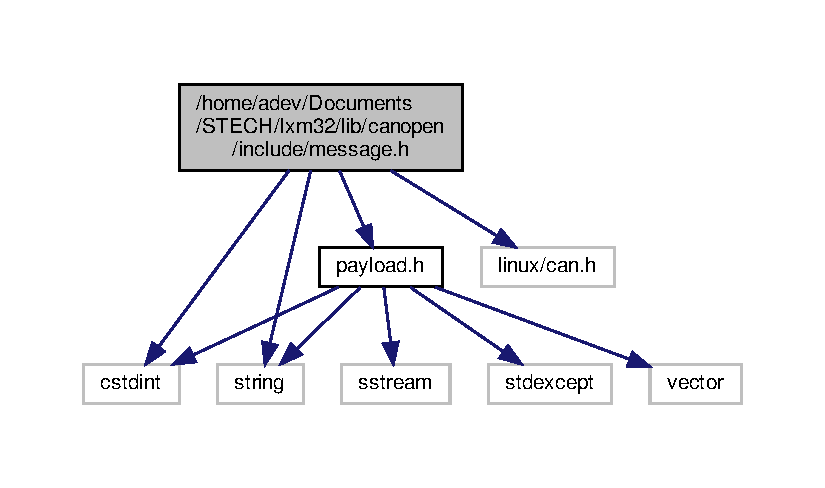
\includegraphics[width=350pt]{message_8h__incl}
\end{center}
\end{figure}
This graph shows which files directly or indirectly include this file\+:\nopagebreak
\begin{figure}[H]
\begin{center}
\leavevmode
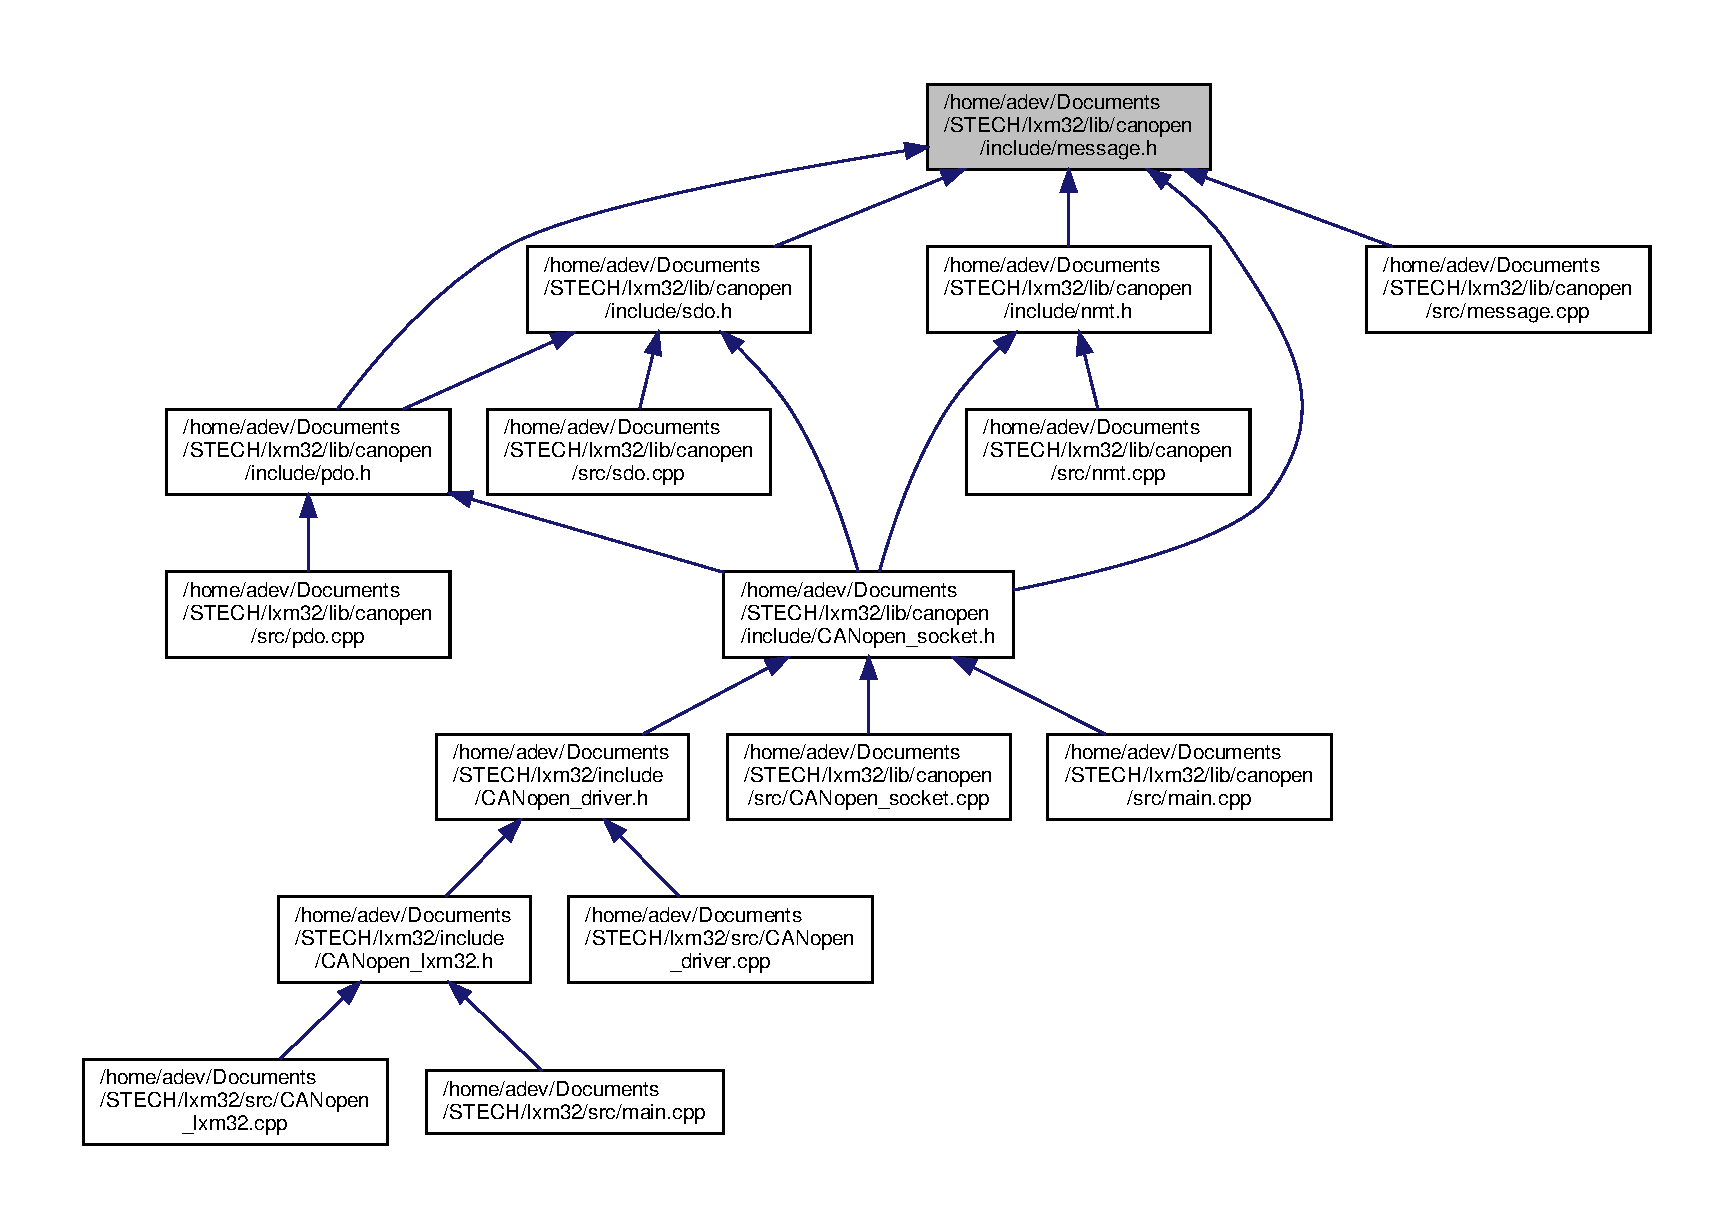
\includegraphics[width=350pt]{message_8h__dep__incl}
\end{center}
\end{figure}
\subsection*{Classes}
\begin{DoxyCompactItemize}
\item 
class \hyperlink{class_c_a_nopen_1_1_message}{C\+A\+Nopen\+::\+Message}
\end{DoxyCompactItemize}
\subsection*{Namespaces}
\begin{DoxyCompactItemize}
\item 
 \hyperlink{namespace_c_a_nopen}{C\+A\+Nopen}
\end{DoxyCompactItemize}

\hypertarget{nmt_8h}{}\section{/home/adev/\+Documents/\+S\+T\+E\+C\+H/lxm32/lib/canopen/include/nmt.h File Reference}
\label{nmt_8h}\index{/home/adev/\+Documents/\+S\+T\+E\+C\+H/lxm32/lib/canopen/include/nmt.\+h@{/home/adev/\+Documents/\+S\+T\+E\+C\+H/lxm32/lib/canopen/include/nmt.\+h}}
{\ttfamily \#include \char`\"{}message.\+h\char`\"{}}\newline
Include dependency graph for nmt.\+h\+:\nopagebreak
\begin{figure}[H]
\begin{center}
\leavevmode
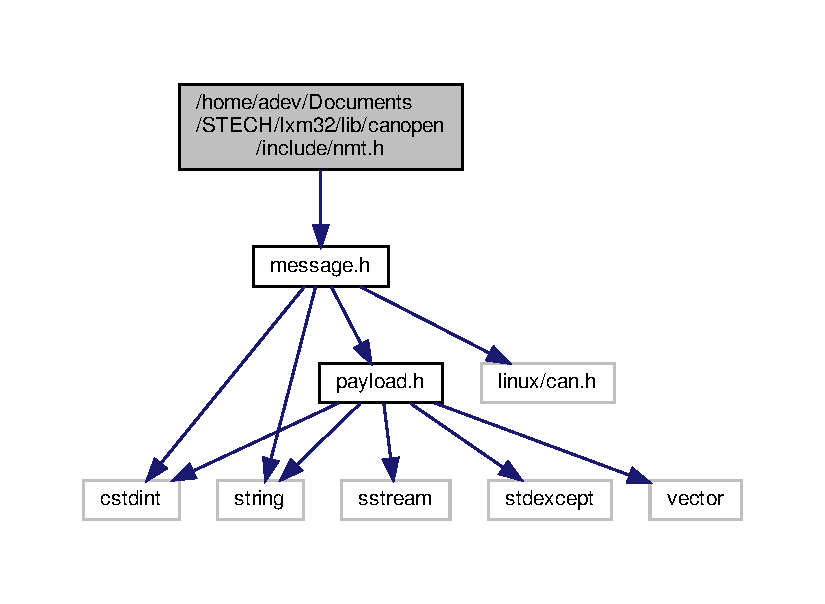
\includegraphics[width=350pt]{nmt_8h__incl}
\end{center}
\end{figure}
This graph shows which files directly or indirectly include this file\+:\nopagebreak
\begin{figure}[H]
\begin{center}
\leavevmode
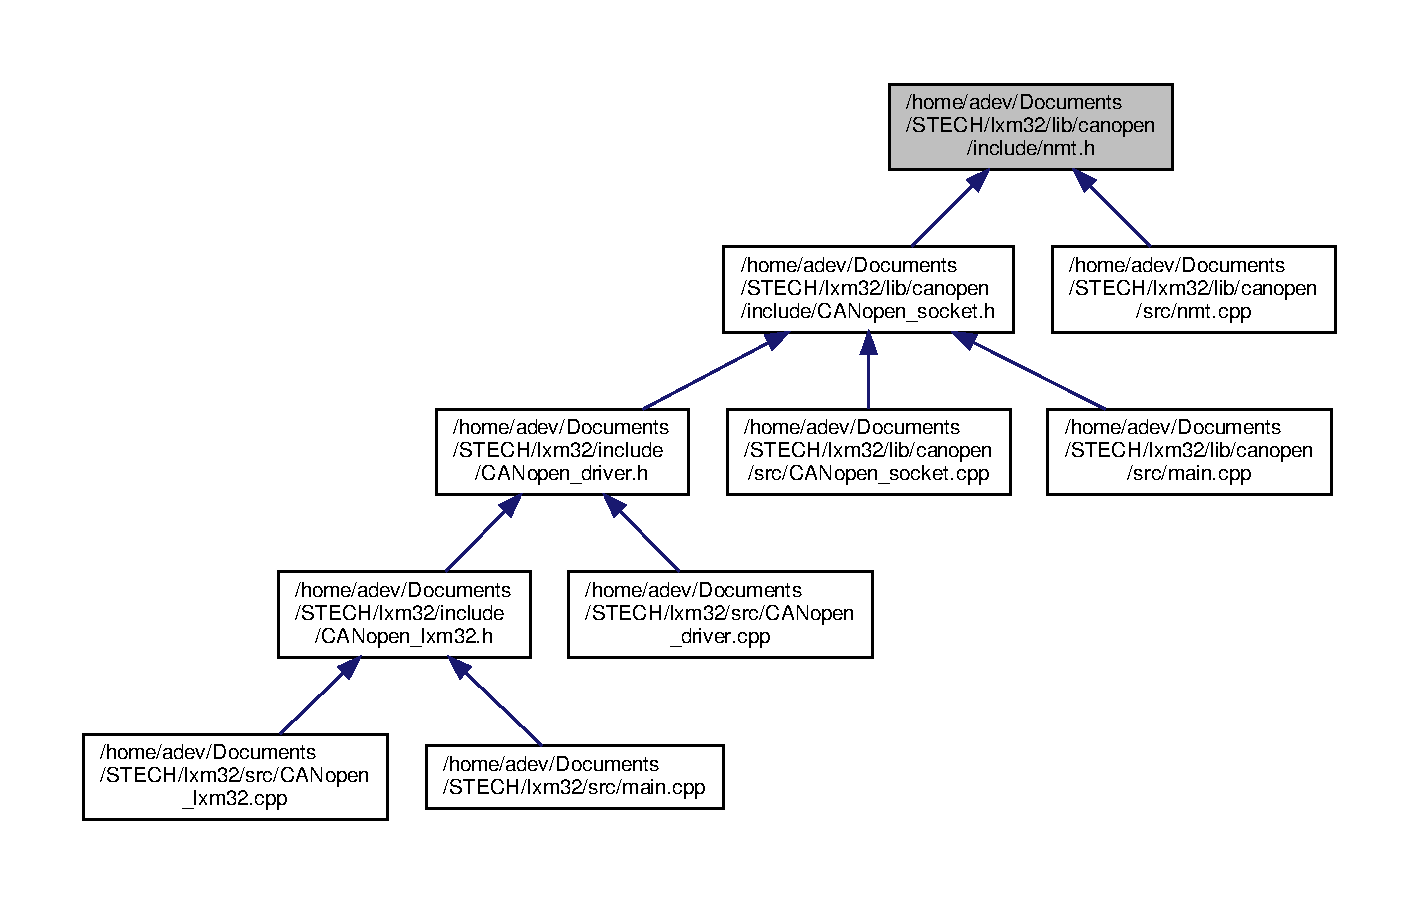
\includegraphics[width=350pt]{nmt_8h__dep__incl}
\end{center}
\end{figure}
\subsection*{Classes}
\begin{DoxyCompactItemize}
\item 
class \hyperlink{class_c_a_nopen_1_1_n_m_t_message}{C\+A\+Nopen\+::\+N\+M\+T\+Message}
\end{DoxyCompactItemize}
\subsection*{Namespaces}
\begin{DoxyCompactItemize}
\item 
 \hyperlink{namespace_c_a_nopen}{C\+A\+Nopen}
\end{DoxyCompactItemize}

\hypertarget{payload_8h}{}\section{/home/adev/\+Documents/\+S\+T\+E\+C\+H/lxm32/lib/canopen/include/payload.h File Reference}
\label{payload_8h}\index{/home/adev/\+Documents/\+S\+T\+E\+C\+H/lxm32/lib/canopen/include/payload.\+h@{/home/adev/\+Documents/\+S\+T\+E\+C\+H/lxm32/lib/canopen/include/payload.\+h}}
{\ttfamily \#include $<$cstdint$>$}\newline
{\ttfamily \#include $<$sstream$>$}\newline
{\ttfamily \#include $<$stdexcept$>$}\newline
{\ttfamily \#include $<$string$>$}\newline
{\ttfamily \#include $<$vector$>$}\newline
Include dependency graph for payload.\+h\+:\nopagebreak
\begin{figure}[H]
\begin{center}
\leavevmode
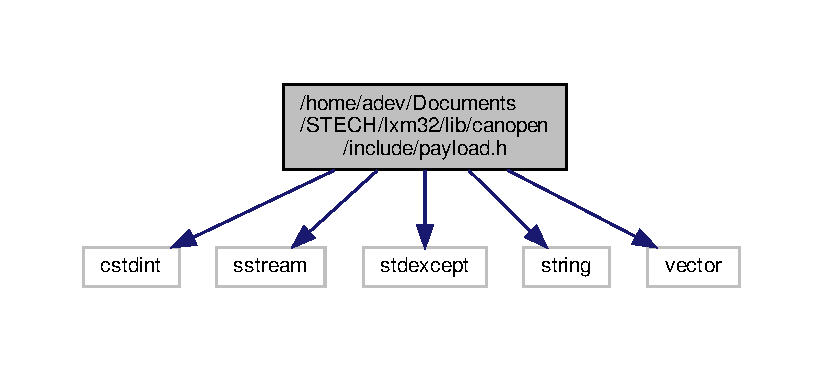
\includegraphics[width=350pt]{payload_8h__incl}
\end{center}
\end{figure}
This graph shows which files directly or indirectly include this file\+:\nopagebreak
\begin{figure}[H]
\begin{center}
\leavevmode
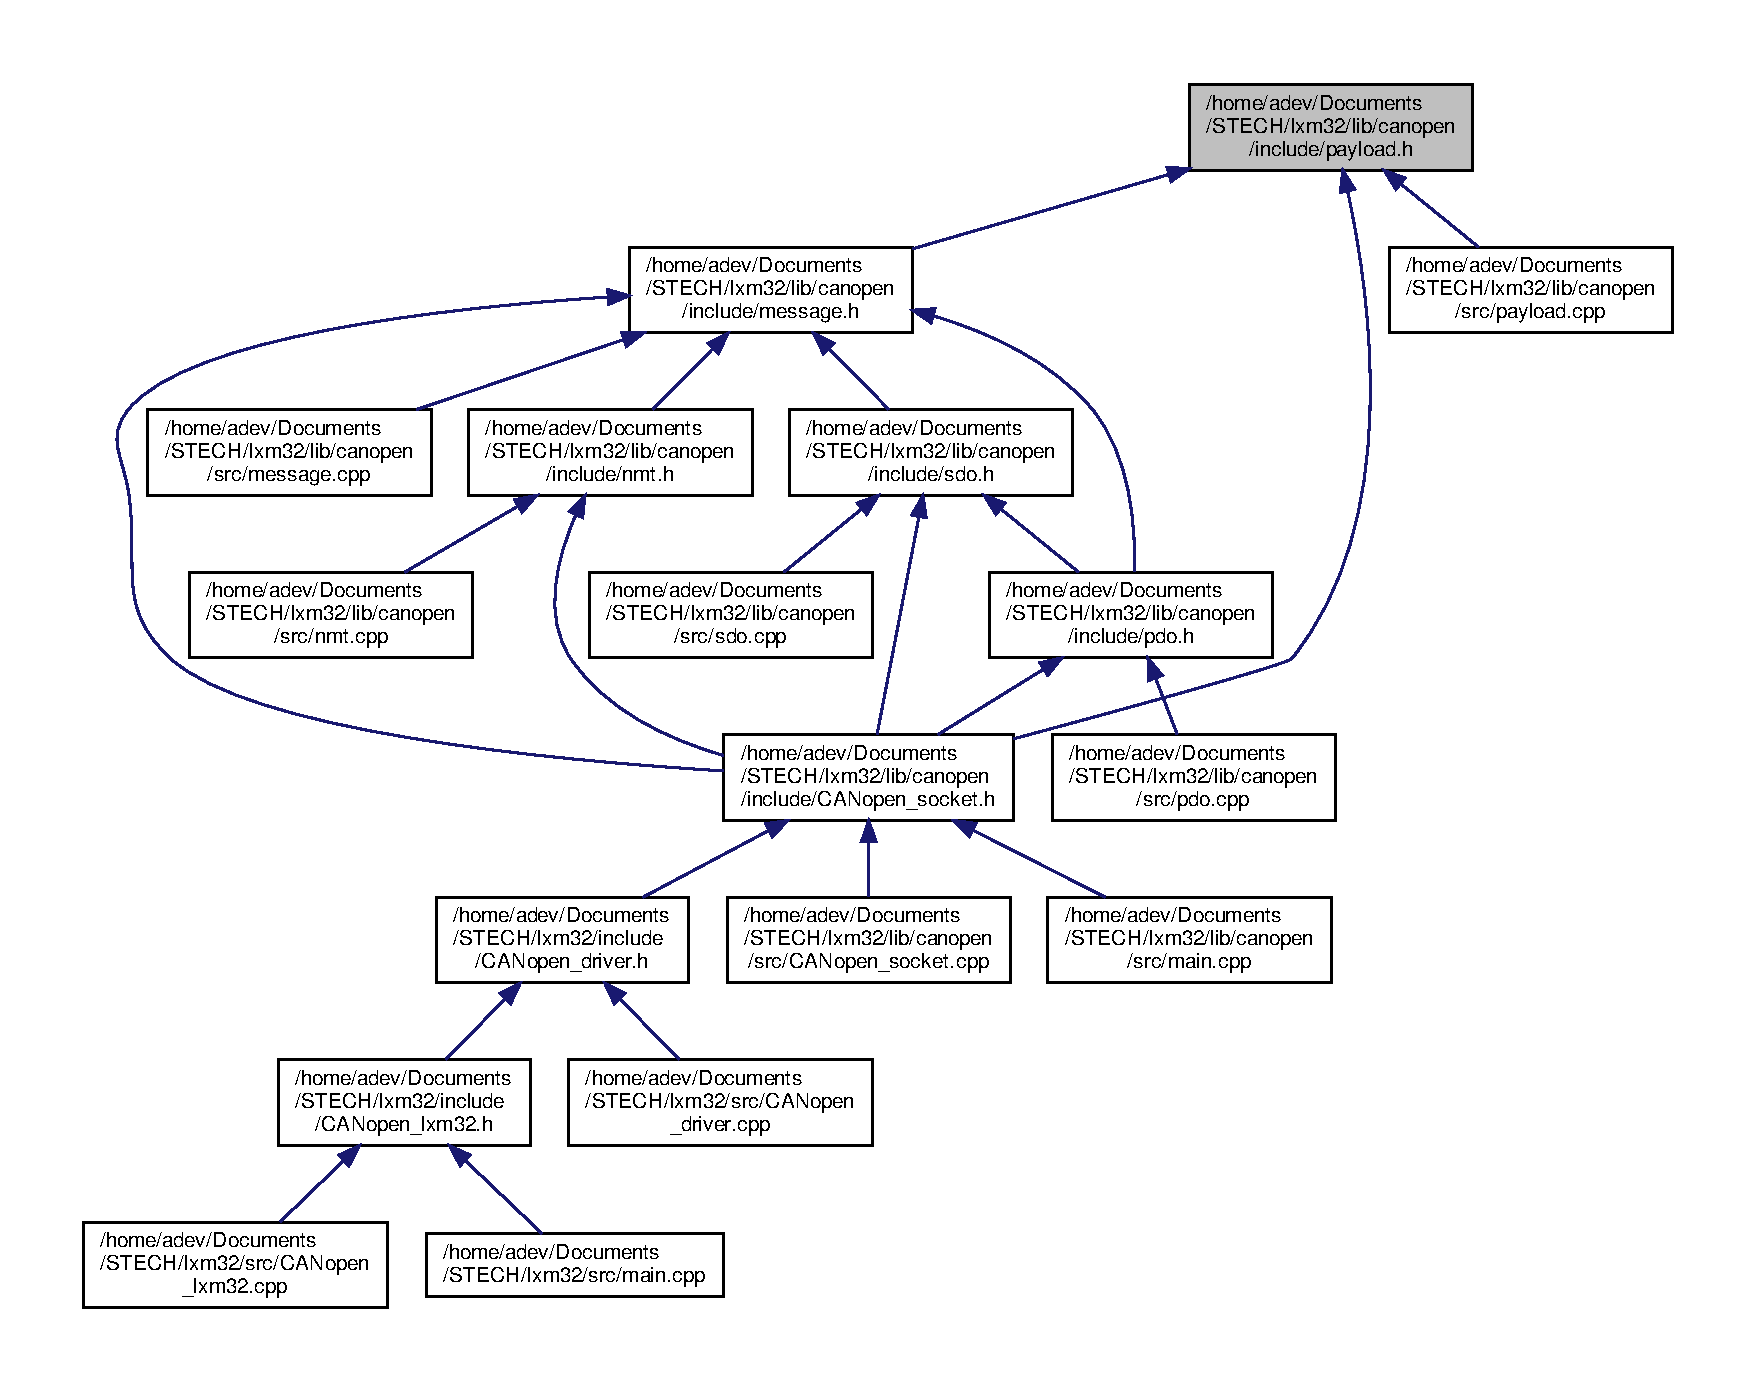
\includegraphics[width=350pt]{payload_8h__dep__incl}
\end{center}
\end{figure}
\subsection*{Classes}
\begin{DoxyCompactItemize}
\item 
class \hyperlink{class_c_a_nopen_1_1_payload}{C\+A\+Nopen\+::\+Payload}
\end{DoxyCompactItemize}
\subsection*{Namespaces}
\begin{DoxyCompactItemize}
\item 
 \hyperlink{namespace_c_a_nopen}{C\+A\+Nopen}
\end{DoxyCompactItemize}
\subsection*{Functions}
\begin{DoxyCompactItemize}
\item 
std\+::ostream \& \hyperlink{payload_8h_ae70f4d583f8731e7bffe4f75957da939}{operator$<$$<$} (std\+::ostream \&out, const \hyperlink{class_c_a_nopen_1_1_payload}{C\+A\+Nopen\+::\+Payload} \&p)
\end{DoxyCompactItemize}


\subsection{Function Documentation}
\mbox{\Hypertarget{payload_8h_ae70f4d583f8731e7bffe4f75957da939}\label{payload_8h_ae70f4d583f8731e7bffe4f75957da939}} 
\index{payload.\+h@{payload.\+h}!operator$<$$<$@{operator$<$$<$}}
\index{operator$<$$<$@{operator$<$$<$}!payload.\+h@{payload.\+h}}
\subsubsection{\texorpdfstring{operator$<$$<$()}{operator<<()}}
{\footnotesize\ttfamily std\+::ostream\& operator$<$$<$ (\begin{DoxyParamCaption}\item[{std\+::ostream \&}]{out,  }\item[{const \hyperlink{class_c_a_nopen_1_1_payload}{C\+A\+Nopen\+::\+Payload} \&}]{p }\end{DoxyParamCaption})}



Definition at line 25 of file payload.\+cpp.


\hypertarget{pdo_8h}{}\section{/home/adev/\+Documents/\+S\+T\+E\+C\+H/lxm32/lib/canopen/include/pdo.h File Reference}
\label{pdo_8h}\index{/home/adev/\+Documents/\+S\+T\+E\+C\+H/lxm32/lib/canopen/include/pdo.\+h@{/home/adev/\+Documents/\+S\+T\+E\+C\+H/lxm32/lib/canopen/include/pdo.\+h}}
{\ttfamily \#include \char`\"{}message.\+h\char`\"{}}\newline
{\ttfamily \#include \char`\"{}sdo.\+h\char`\"{}}\newline
Include dependency graph for pdo.\+h\+:\nopagebreak
\begin{figure}[H]
\begin{center}
\leavevmode
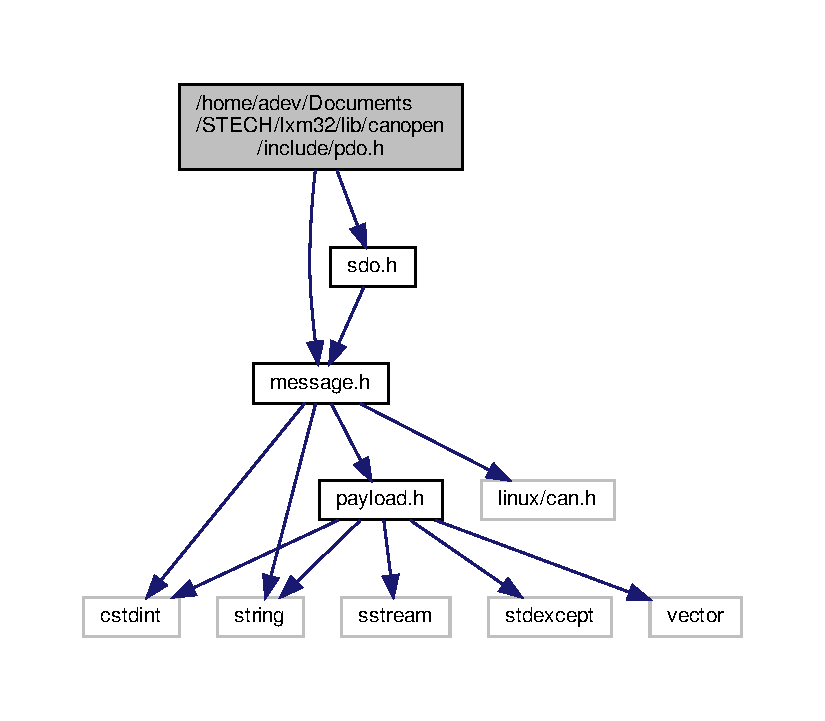
\includegraphics[width=350pt]{pdo_8h__incl}
\end{center}
\end{figure}
This graph shows which files directly or indirectly include this file\+:\nopagebreak
\begin{figure}[H]
\begin{center}
\leavevmode
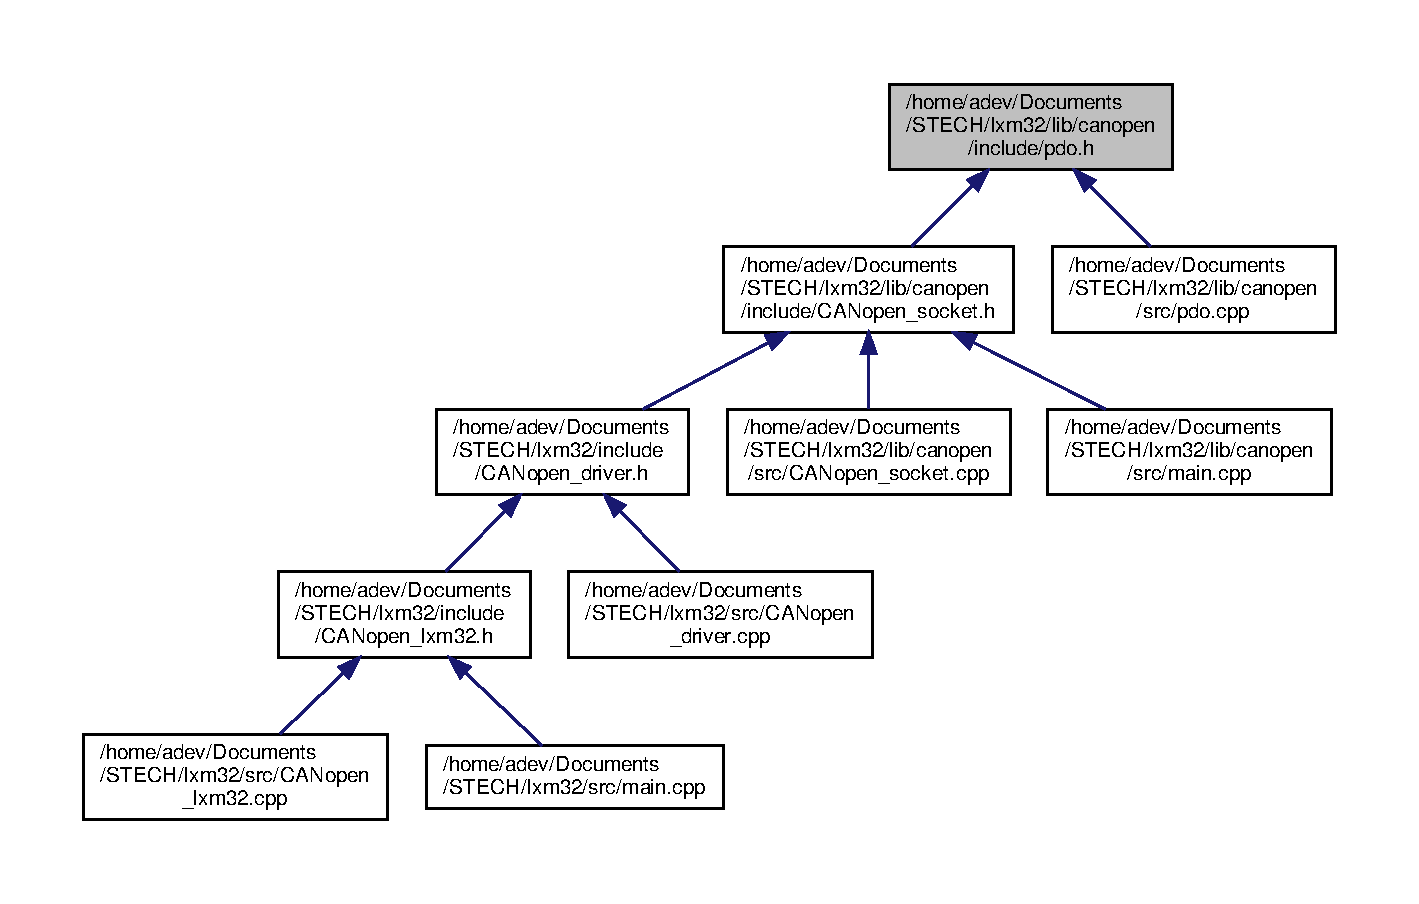
\includegraphics[width=350pt]{pdo_8h__dep__incl}
\end{center}
\end{figure}
\subsection*{Classes}
\begin{DoxyCompactItemize}
\item 
class \hyperlink{class_c_a_nopen_1_1_p_d_o_message}{C\+A\+Nopen\+::\+P\+D\+O\+Message}
\end{DoxyCompactItemize}
\subsection*{Namespaces}
\begin{DoxyCompactItemize}
\item 
 \hyperlink{namespace_c_a_nopen}{C\+A\+Nopen}
\end{DoxyCompactItemize}

\hypertarget{sdo_8h}{}\section{/home/adev/\+Documents/\+S\+T\+E\+C\+H/lxm32/lib/canopen/include/sdo.h File Reference}
\label{sdo_8h}\index{/home/adev/\+Documents/\+S\+T\+E\+C\+H/lxm32/lib/canopen/include/sdo.\+h@{/home/adev/\+Documents/\+S\+T\+E\+C\+H/lxm32/lib/canopen/include/sdo.\+h}}
{\ttfamily \#include \char`\"{}message.\+h\char`\"{}}\newline
Include dependency graph for sdo.\+h\+:\nopagebreak
\begin{figure}[H]
\begin{center}
\leavevmode
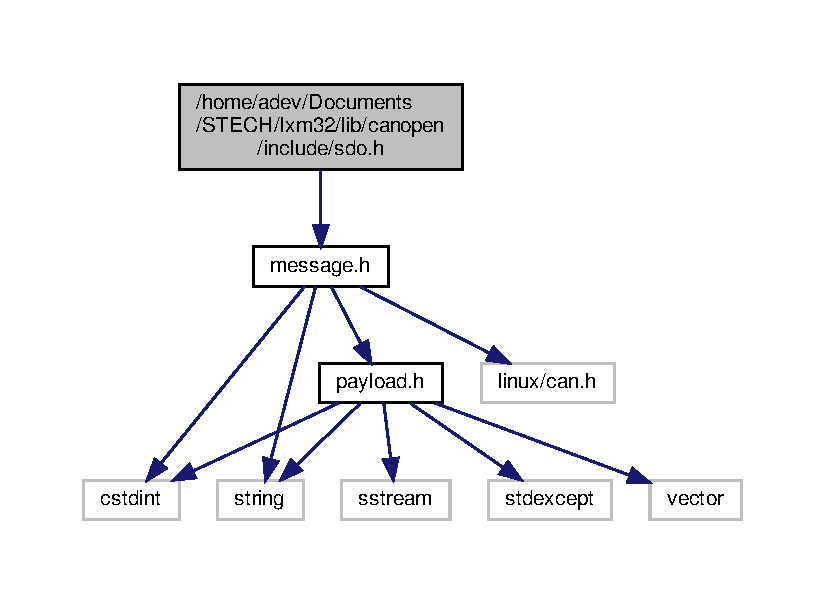
\includegraphics[width=350pt]{sdo_8h__incl}
\end{center}
\end{figure}
This graph shows which files directly or indirectly include this file\+:\nopagebreak
\begin{figure}[H]
\begin{center}
\leavevmode
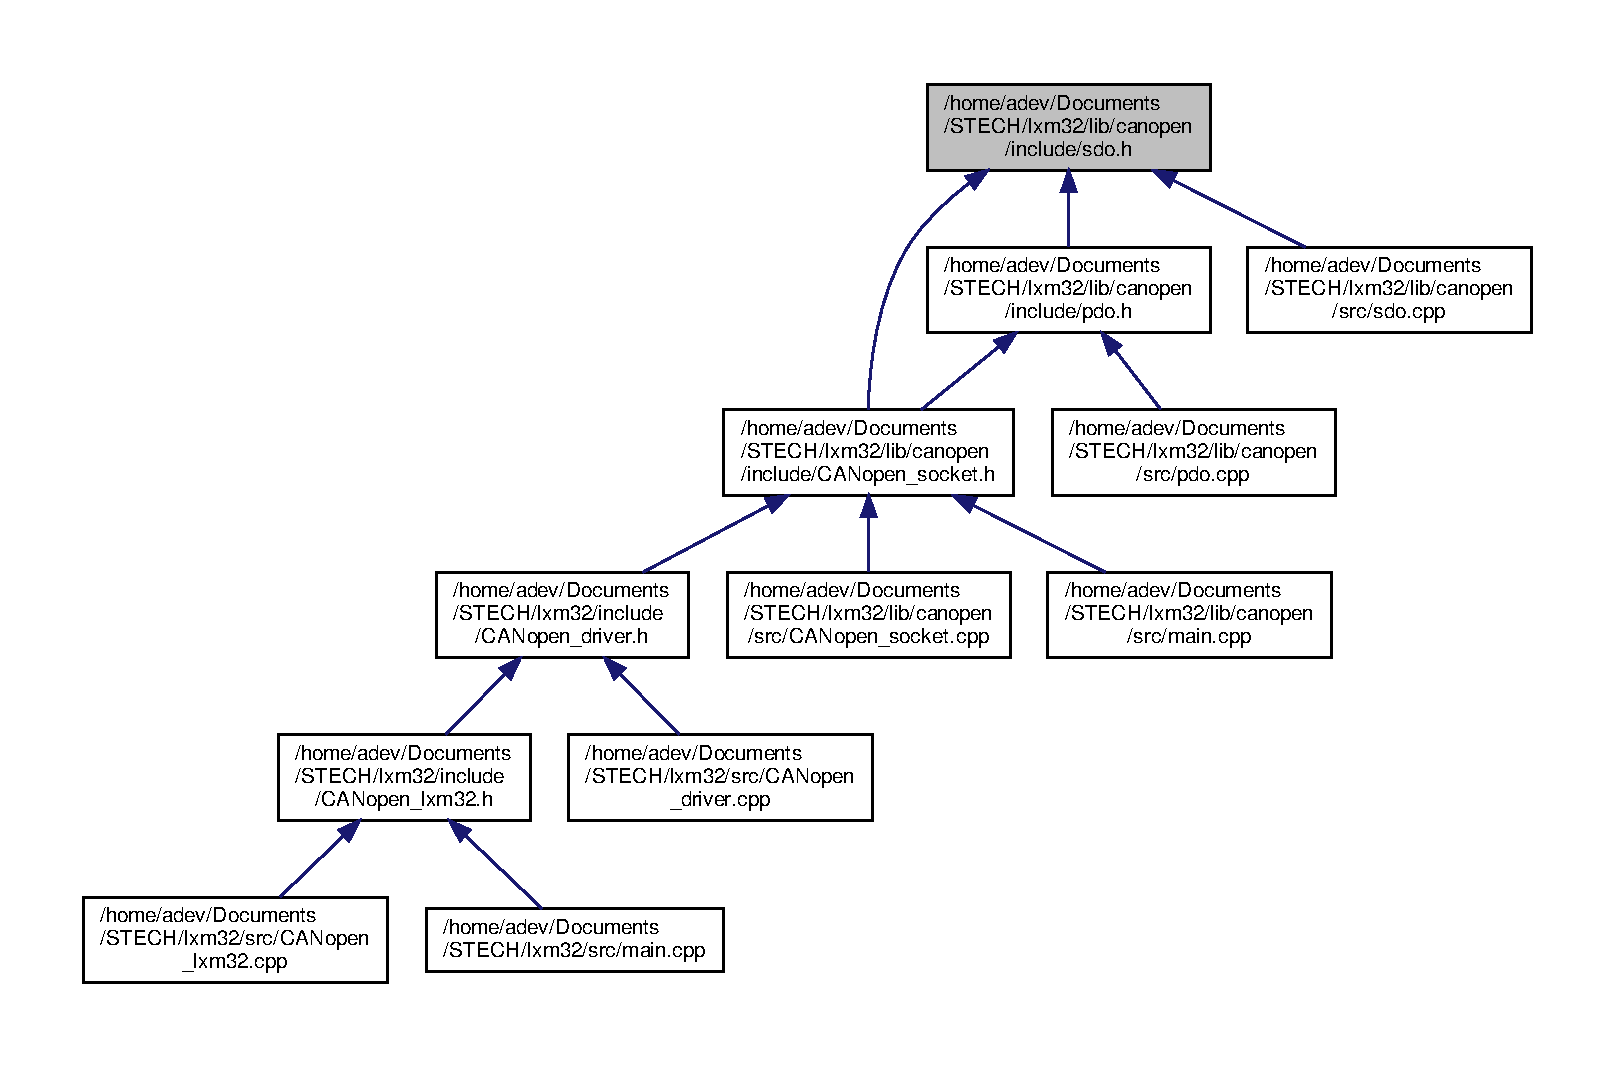
\includegraphics[width=350pt]{sdo_8h__dep__incl}
\end{center}
\end{figure}
\subsection*{Classes}
\begin{DoxyCompactItemize}
\item 
class \hyperlink{class_c_a_nopen_1_1_s_d_o_message}{C\+A\+Nopen\+::\+S\+D\+O\+Message}
\item 
class \hyperlink{class_c_a_nopen_1_1_s_d_o_inbound}{C\+A\+Nopen\+::\+S\+D\+O\+Inbound}
\item 
class \hyperlink{class_c_a_nopen_1_1_s_d_o_outbound}{C\+A\+Nopen\+::\+S\+D\+O\+Outbound}
\item 
class \hyperlink{class_c_a_nopen_1_1_s_d_o_outbound_read}{C\+A\+Nopen\+::\+S\+D\+O\+Outbound\+Read}
\item 
class \hyperlink{class_c_a_nopen_1_1_s_d_o_outbound_write}{C\+A\+Nopen\+::\+S\+D\+O\+Outbound\+Write}
\end{DoxyCompactItemize}
\subsection*{Namespaces}
\begin{DoxyCompactItemize}
\item 
 \hyperlink{namespace_c_a_nopen}{C\+A\+Nopen}
\end{DoxyCompactItemize}

\hypertarget{lib_2canopen_2_r_e_a_d_m_e_8md}{}\section{/home/adev/\+Documents/\+S\+T\+E\+C\+H/lxm32/lib/canopen/\+R\+E\+A\+D\+ME.md File Reference}
\label{lib_2canopen_2_r_e_a_d_m_e_8md}\index{/home/adev/\+Documents/\+S\+T\+E\+C\+H/lxm32/lib/canopen/\+R\+E\+A\+D\+M\+E.\+md@{/home/adev/\+Documents/\+S\+T\+E\+C\+H/lxm32/lib/canopen/\+R\+E\+A\+D\+M\+E.\+md}}

\hypertarget{lib_2joystick_2_r_e_a_d_m_e_8md}{}\section{/home/adev/\+Documents/\+S\+T\+E\+C\+H/lxm32/lib/joystick/\+R\+E\+A\+D\+ME.md File Reference}
\label{lib_2joystick_2_r_e_a_d_m_e_8md}\index{/home/adev/\+Documents/\+S\+T\+E\+C\+H/lxm32/lib/joystick/\+R\+E\+A\+D\+M\+E.\+md@{/home/adev/\+Documents/\+S\+T\+E\+C\+H/lxm32/lib/joystick/\+R\+E\+A\+D\+M\+E.\+md}}

\hypertarget{_r_e_a_d_m_e_8md}{}\section{/home/adev/\+Documents/\+S\+T\+E\+C\+H/lxm32/\+R\+E\+A\+D\+ME.md File Reference}
\label{_r_e_a_d_m_e_8md}\index{/home/adev/\+Documents/\+S\+T\+E\+C\+H/lxm32/\+R\+E\+A\+D\+M\+E.\+md@{/home/adev/\+Documents/\+S\+T\+E\+C\+H/lxm32/\+R\+E\+A\+D\+M\+E.\+md}}

\hypertarget{_c_a_nopen__socket_8cpp}{}\section{/home/adev/\+Documents/\+S\+T\+E\+C\+H/lxm32/lib/canopen/src/\+C\+A\+Nopen\+\_\+socket.cpp File Reference}
\label{_c_a_nopen__socket_8cpp}\index{/home/adev/\+Documents/\+S\+T\+E\+C\+H/lxm32/lib/canopen/src/\+C\+A\+Nopen\+\_\+socket.\+cpp@{/home/adev/\+Documents/\+S\+T\+E\+C\+H/lxm32/lib/canopen/src/\+C\+A\+Nopen\+\_\+socket.\+cpp}}
{\ttfamily \#include \char`\"{}C\+A\+Nopen\+\_\+socket.\+h\char`\"{}}\newline
{\ttfamily \#include $<$iostream$>$}\newline
{\ttfamily \#include $<$linux/can/raw.\+h$>$}\newline
{\ttfamily \#include $<$net/if.\+h$>$}\newline
{\ttfamily \#include $<$stdexcept$>$}\newline
{\ttfamily \#include $<$stdio.\+h$>$}\newline
{\ttfamily \#include $<$string.\+h$>$}\newline
{\ttfamily \#include $<$sys/ioctl.\+h$>$}\newline
{\ttfamily \#include $<$sys/socket.\+h$>$}\newline
{\ttfamily \#include $<$sys/types.\+h$>$}\newline
{\ttfamily \#include $<$unistd.\+h$>$}\newline
Include dependency graph for C\+A\+Nopen\+\_\+socket.\+cpp\+:\nopagebreak
\begin{figure}[H]
\begin{center}
\leavevmode
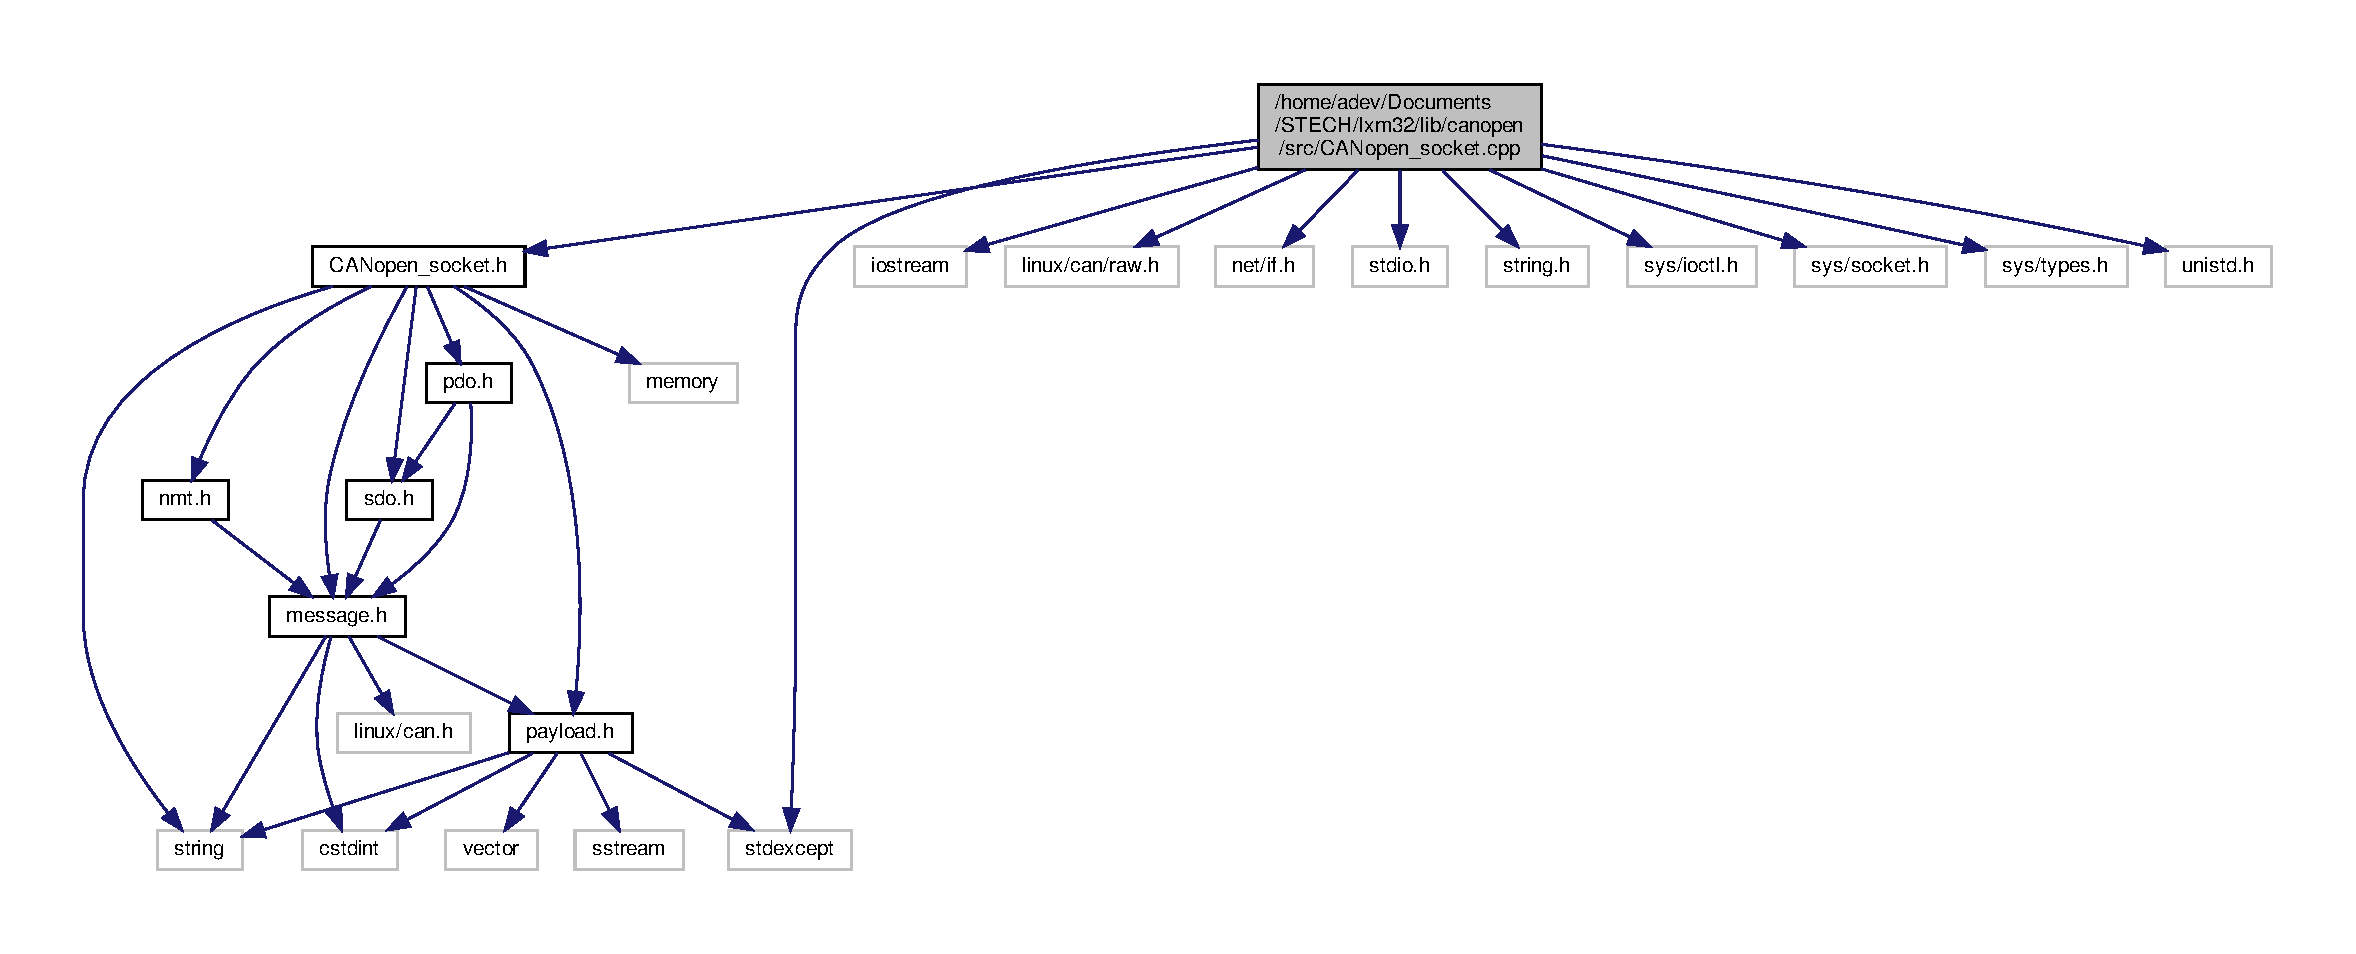
\includegraphics[width=350pt]{_c_a_nopen__socket_8cpp__incl}
\end{center}
\end{figure}
\subsection*{Namespaces}
\begin{DoxyCompactItemize}
\item 
 \hyperlink{namespace_c_a_nopen}{C\+A\+Nopen}
\end{DoxyCompactItemize}

\hypertarget{lib_2canopen_2src_2main_8cpp}{}\section{/home/adev/\+Documents/\+S\+T\+E\+C\+H/lxm32/lib/canopen/src/main.cpp File Reference}
\label{lib_2canopen_2src_2main_8cpp}\index{/home/adev/\+Documents/\+S\+T\+E\+C\+H/lxm32/lib/canopen/src/main.\+cpp@{/home/adev/\+Documents/\+S\+T\+E\+C\+H/lxm32/lib/canopen/src/main.\+cpp}}
{\ttfamily \#include \char`\"{}C\+A\+Nopen\+\_\+socket.\+h\char`\"{}}\newline
{\ttfamily \#include $<$iostream$>$}\newline
Include dependency graph for main.\+cpp\+:\nopagebreak
\begin{figure}[H]
\begin{center}
\leavevmode
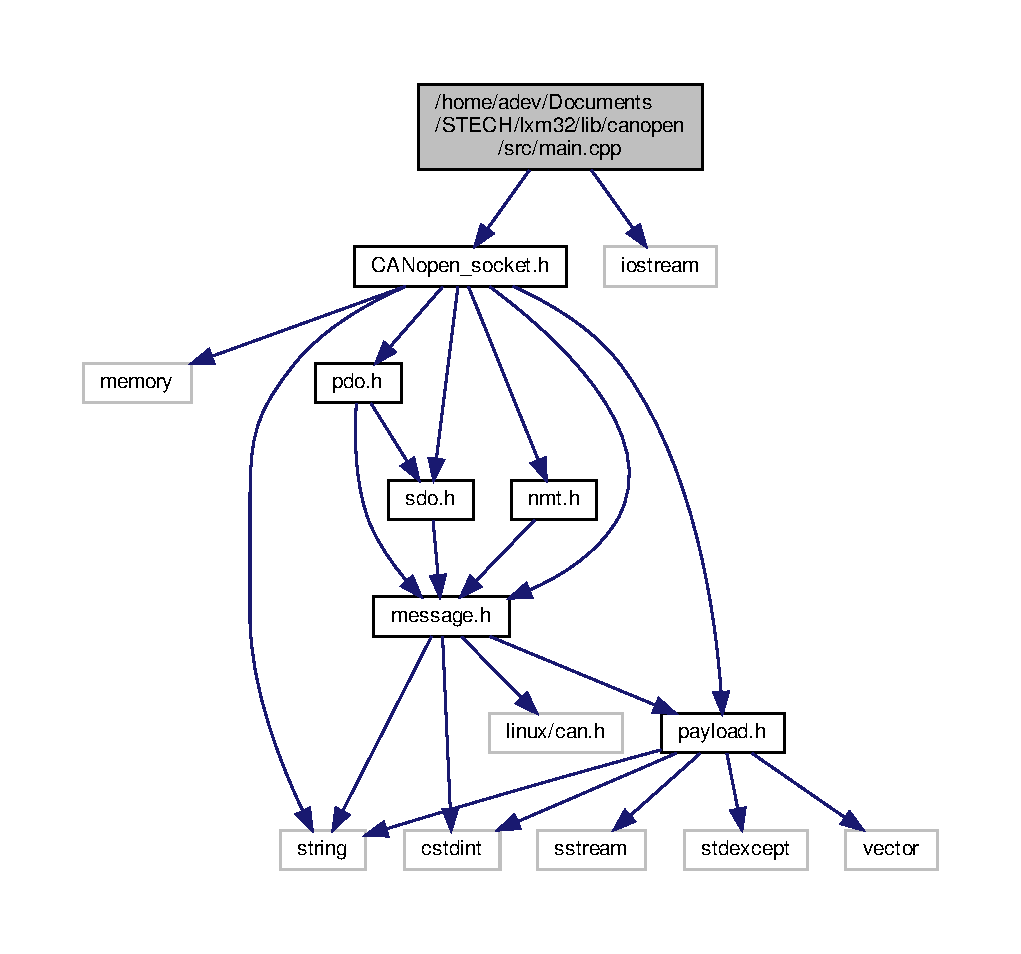
\includegraphics[width=350pt]{lib_2canopen_2src_2main_8cpp__incl}
\end{center}
\end{figure}
\subsection*{Classes}
\begin{DoxyCompactItemize}
\item 
struct \hyperlink{structsss}{sss$<$ T $>$}
\end{DoxyCompactItemize}
\subsection*{Functions}
\begin{DoxyCompactItemize}
\item 
void \hyperlink{lib_2canopen_2src_2main_8cpp_ad179db7b04bfd86a67a6a62a36bffdac}{usage} (char $\ast$$\ast$argv)
\item 
int \hyperlink{lib_2canopen_2src_2main_8cpp_a3c04138a5bfe5d72780bb7e82a18e627}{main} (int argc, char $\ast$$\ast$argv)
\end{DoxyCompactItemize}


\subsection{Function Documentation}
\mbox{\Hypertarget{lib_2canopen_2src_2main_8cpp_a3c04138a5bfe5d72780bb7e82a18e627}\label{lib_2canopen_2src_2main_8cpp_a3c04138a5bfe5d72780bb7e82a18e627}} 
\index{lib/canopen/src/main.\+cpp@{lib/canopen/src/main.\+cpp}!main@{main}}
\index{main@{main}!lib/canopen/src/main.\+cpp@{lib/canopen/src/main.\+cpp}}
\subsubsection{\texorpdfstring{main()}{main()}}
{\footnotesize\ttfamily int main (\begin{DoxyParamCaption}\item[{int}]{argc,  }\item[{char $\ast$$\ast$}]{argv }\end{DoxyParamCaption})}



Definition at line 23 of file main.\+cpp.

\mbox{\Hypertarget{lib_2canopen_2src_2main_8cpp_ad179db7b04bfd86a67a6a62a36bffdac}\label{lib_2canopen_2src_2main_8cpp_ad179db7b04bfd86a67a6a62a36bffdac}} 
\index{lib/canopen/src/main.\+cpp@{lib/canopen/src/main.\+cpp}!usage@{usage}}
\index{usage@{usage}!lib/canopen/src/main.\+cpp@{lib/canopen/src/main.\+cpp}}
\subsubsection{\texorpdfstring{usage()}{usage()}}
{\footnotesize\ttfamily void usage (\begin{DoxyParamCaption}\item[{char $\ast$$\ast$}]{argv }\end{DoxyParamCaption})}



Definition at line 5 of file main.\+cpp.


\hypertarget{lib_2joystick_2src_2main_8cpp}{}\section{/home/adev/\+Documents/\+S\+T\+E\+C\+H/lxm32/lib/joystick/src/main.cpp File Reference}
\label{lib_2joystick_2src_2main_8cpp}\index{/home/adev/\+Documents/\+S\+T\+E\+C\+H/lxm32/lib/joystick/src/main.\+cpp@{/home/adev/\+Documents/\+S\+T\+E\+C\+H/lxm32/lib/joystick/src/main.\+cpp}}
{\ttfamily \#include \char`\"{}joystick.\+h\char`\"{}}\newline
{\ttfamily \#include $<$iostream$>$}\newline
Include dependency graph for main.\+cpp\+:\nopagebreak
\begin{figure}[H]
\begin{center}
\leavevmode
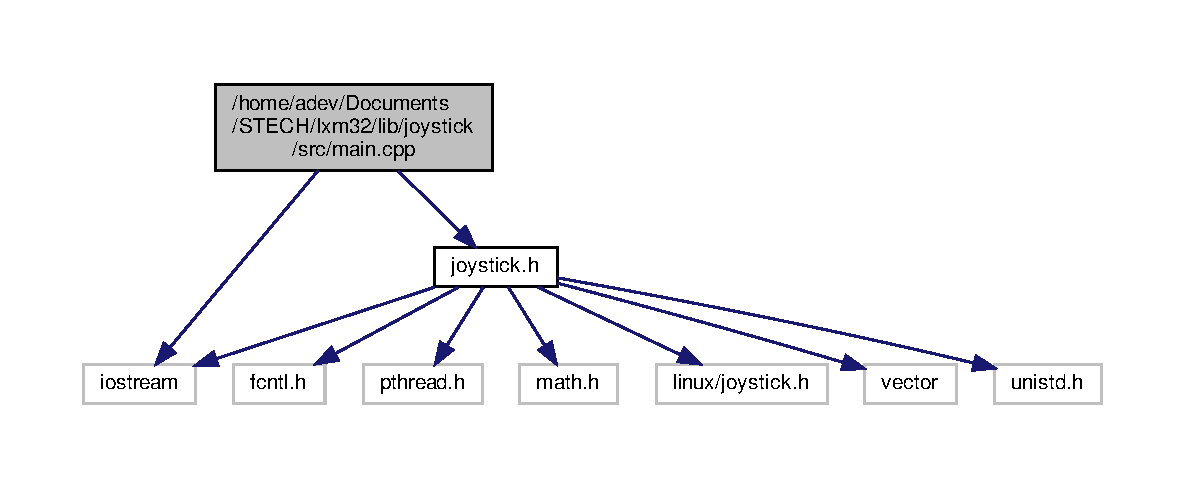
\includegraphics[width=350pt]{lib_2joystick_2src_2main_8cpp__incl}
\end{center}
\end{figure}
\subsection*{Functions}
\begin{DoxyCompactItemize}
\item 
int \hyperlink{lib_2joystick_2src_2main_8cpp_ae66f6b31b5ad750f1fe042a706a4e3d4}{main} ()
\end{DoxyCompactItemize}


\subsection{Function Documentation}
\mbox{\Hypertarget{lib_2joystick_2src_2main_8cpp_ae66f6b31b5ad750f1fe042a706a4e3d4}\label{lib_2joystick_2src_2main_8cpp_ae66f6b31b5ad750f1fe042a706a4e3d4}} 
\index{lib/joystick/src/main.\+cpp@{lib/joystick/src/main.\+cpp}!main@{main}}
\index{main@{main}!lib/joystick/src/main.\+cpp@{lib/joystick/src/main.\+cpp}}
\subsubsection{\texorpdfstring{main()}{main()}}
{\footnotesize\ttfamily int main (\begin{DoxyParamCaption}{ }\end{DoxyParamCaption})}



Definition at line 3 of file main.\+cpp.


\hypertarget{src_2main_8cpp}{}\section{/home/adev/\+Documents/\+S\+T\+E\+C\+H/lxm32/src/main.cpp File Reference}
\label{src_2main_8cpp}\index{/home/adev/\+Documents/\+S\+T\+E\+C\+H/lxm32/src/main.\+cpp@{/home/adev/\+Documents/\+S\+T\+E\+C\+H/lxm32/src/main.\+cpp}}
{\ttfamily \#include $<$stdio.\+h$>$}\newline
{\ttfamily \#include $<$stdlib.\+h$>$}\newline
{\ttfamily \#include $<$unistd.\+h$>$}\newline
{\ttfamily \#include $<$string.\+h$>$}\newline
{\ttfamily \#include $<$cstdint$>$}\newline
{\ttfamily \#include $<$net/if.\+h$>$}\newline
{\ttfamily \#include $<$sys/types.\+h$>$}\newline
{\ttfamily \#include $<$sys/socket.\+h$>$}\newline
{\ttfamily \#include $<$sys/ioctl.\+h$>$}\newline
{\ttfamily \#include $<$linux/can.\+h$>$}\newline
{\ttfamily \#include $<$linux/can/raw.\+h$>$}\newline
{\ttfamily \#include \char`\"{}C\+A\+Nopen\+\_\+lxm32.\+h\char`\"{}}\newline
{\ttfamily \#include \char`\"{}joystick.\+h\char`\"{}}\newline
Include dependency graph for main.\+cpp\+:\nopagebreak
\begin{figure}[H]
\begin{center}
\leavevmode
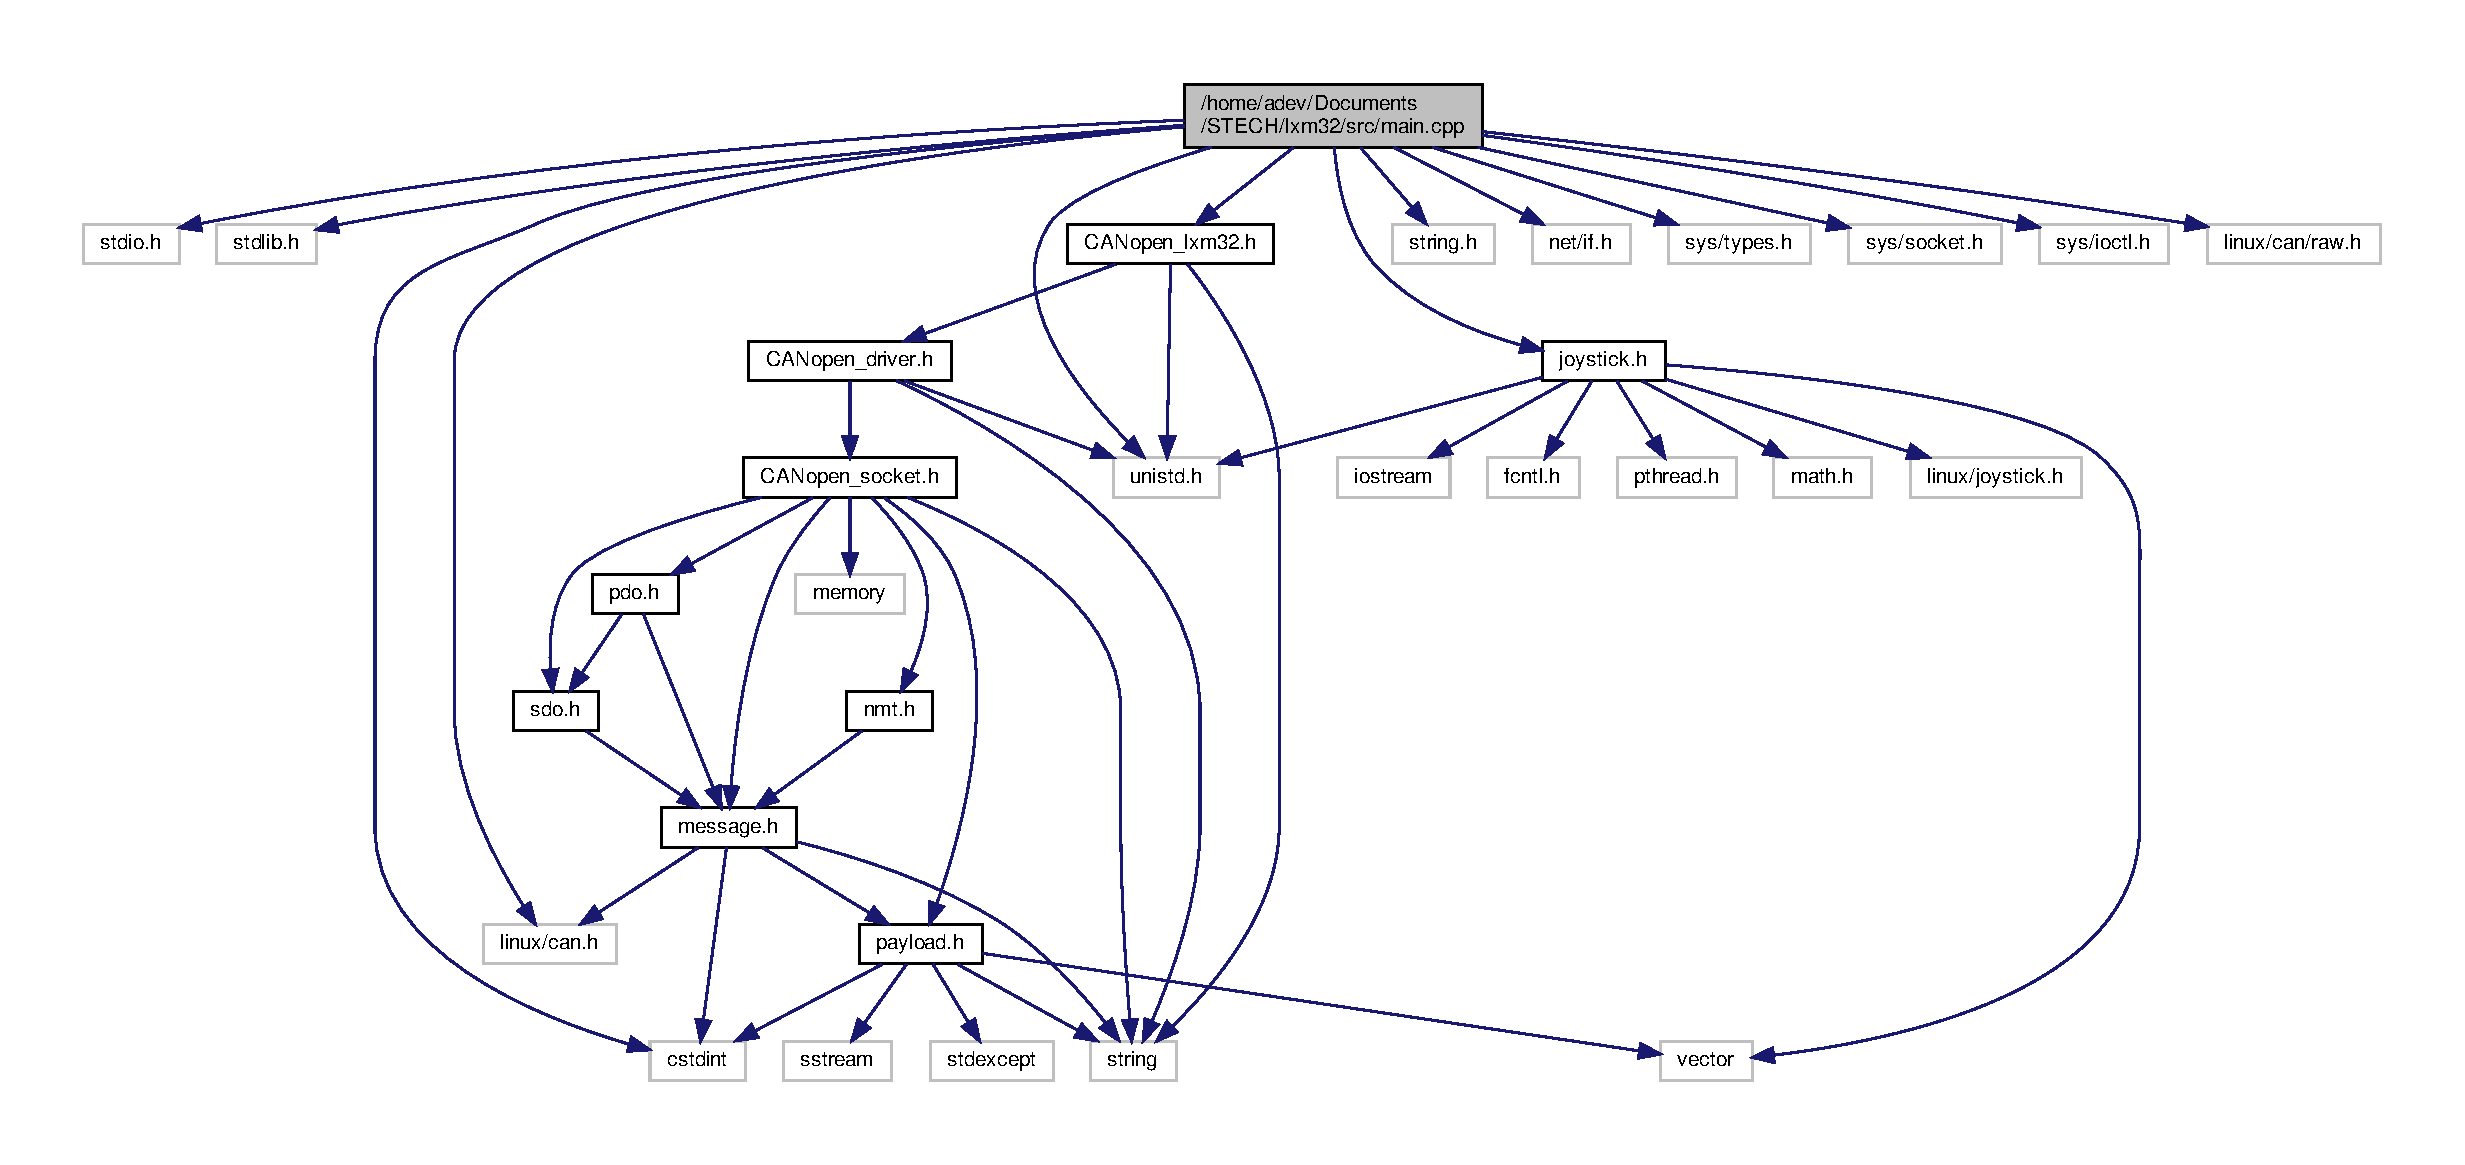
\includegraphics[width=350pt]{src_2main_8cpp__incl}
\end{center}
\end{figure}
\subsection*{Functions}
\begin{DoxyCompactItemize}
\item 
int \hyperlink{src_2main_8cpp_a3c04138a5bfe5d72780bb7e82a18e627}{main} (int argc, char $\ast$$\ast$argv)
\end{DoxyCompactItemize}


\subsection{Function Documentation}
\mbox{\Hypertarget{src_2main_8cpp_a3c04138a5bfe5d72780bb7e82a18e627}\label{src_2main_8cpp_a3c04138a5bfe5d72780bb7e82a18e627}} 
\index{src/main.\+cpp@{src/main.\+cpp}!main@{main}}
\index{main@{main}!src/main.\+cpp@{src/main.\+cpp}}
\subsubsection{\texorpdfstring{main()}{main()}}
{\footnotesize\ttfamily int main (\begin{DoxyParamCaption}\item[{int}]{argc,  }\item[{char $\ast$$\ast$}]{argv }\end{DoxyParamCaption})}



Definition at line 22 of file main.\+cpp.


\hypertarget{message_8cpp}{}\section{/home/adev/\+Documents/\+S\+T\+E\+C\+H/lxm32/lib/canopen/src/message.cpp File Reference}
\label{message_8cpp}\index{/home/adev/\+Documents/\+S\+T\+E\+C\+H/lxm32/lib/canopen/src/message.\+cpp@{/home/adev/\+Documents/\+S\+T\+E\+C\+H/lxm32/lib/canopen/src/message.\+cpp}}
{\ttfamily \#include \char`\"{}message.\+h\char`\"{}}\newline
{\ttfamily \#include $<$sstream$>$}\newline
{\ttfamily \#include $<$string.\+h$>$}\newline
Include dependency graph for message.\+cpp\+:\nopagebreak
\begin{figure}[H]
\begin{center}
\leavevmode
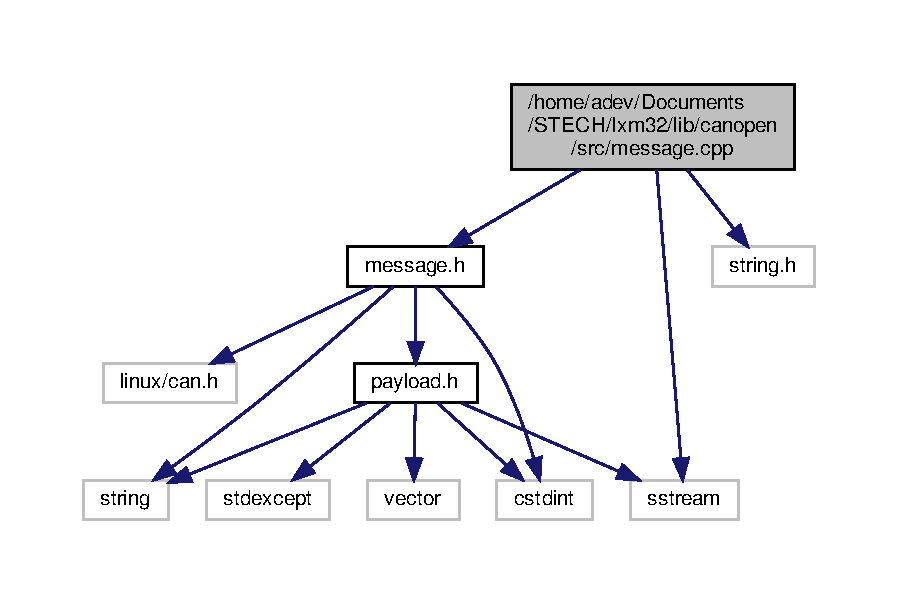
\includegraphics[width=350pt]{message_8cpp__incl}
\end{center}
\end{figure}
\subsection*{Namespaces}
\begin{DoxyCompactItemize}
\item 
 \hyperlink{namespace_c_a_nopen}{C\+A\+Nopen}
\end{DoxyCompactItemize}

\hypertarget{nmt_8cpp}{}\section{/home/adev/\+Documents/\+S\+T\+E\+C\+H/lxm32/lib/canopen/src/nmt.cpp File Reference}
\label{nmt_8cpp}\index{/home/adev/\+Documents/\+S\+T\+E\+C\+H/lxm32/lib/canopen/src/nmt.\+cpp@{/home/adev/\+Documents/\+S\+T\+E\+C\+H/lxm32/lib/canopen/src/nmt.\+cpp}}
{\ttfamily \#include \char`\"{}nmt.\+h\char`\"{}}\newline
Include dependency graph for nmt.\+cpp\+:\nopagebreak
\begin{figure}[H]
\begin{center}
\leavevmode
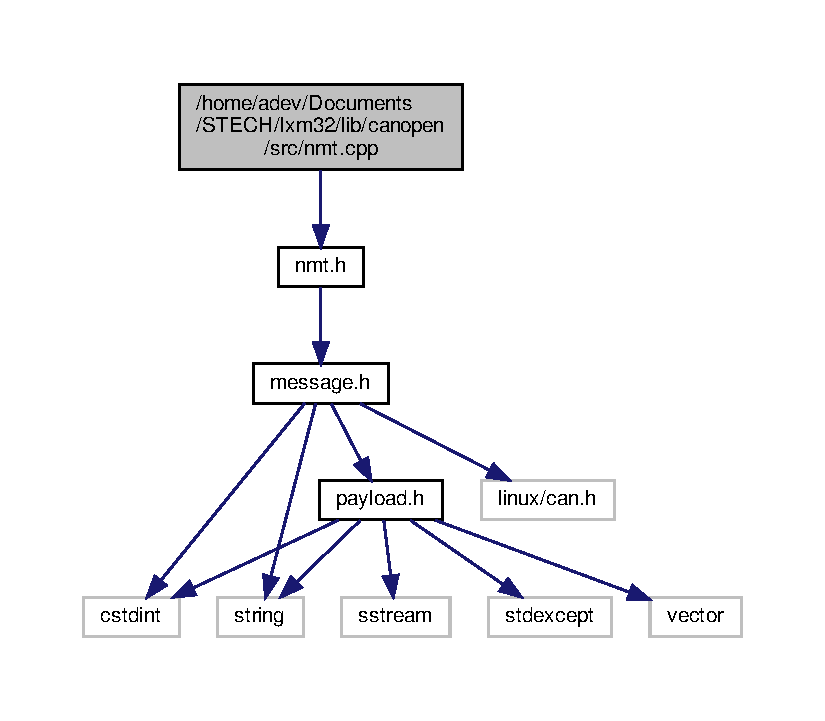
\includegraphics[width=350pt]{nmt_8cpp__incl}
\end{center}
\end{figure}
\subsection*{Namespaces}
\begin{DoxyCompactItemize}
\item 
 \hyperlink{namespace_c_a_nopen}{C\+A\+Nopen}
\end{DoxyCompactItemize}

\hypertarget{payload_8cpp}{}\section{/home/adev/\+Documents/\+S\+T\+E\+C\+H/lxm32/lib/canopen/src/payload.cpp File Reference}
\label{payload_8cpp}\index{/home/adev/\+Documents/\+S\+T\+E\+C\+H/lxm32/lib/canopen/src/payload.\+cpp@{/home/adev/\+Documents/\+S\+T\+E\+C\+H/lxm32/lib/canopen/src/payload.\+cpp}}
{\ttfamily \#include \char`\"{}payload.\+h\char`\"{}}\newline
{\ttfamily \#include $<$ostream$>$}\newline
{\ttfamily \#include $<$iomanip$>$}\newline
Include dependency graph for payload.\+cpp\+:\nopagebreak
\begin{figure}[H]
\begin{center}
\leavevmode
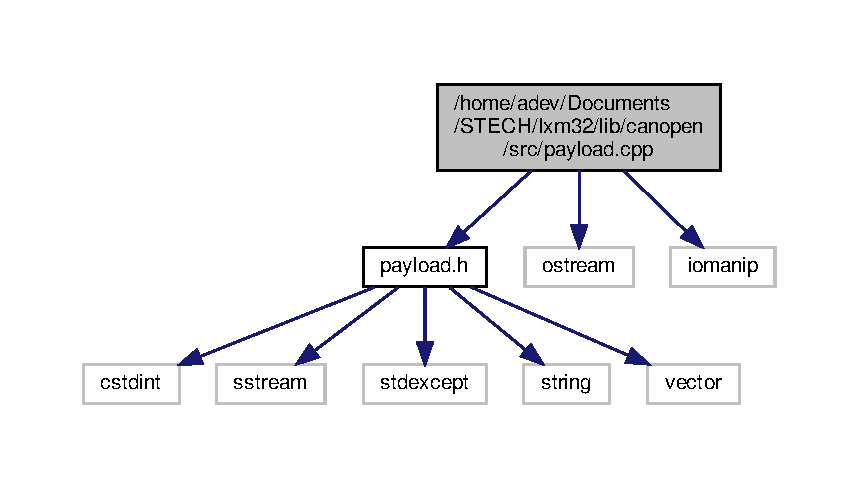
\includegraphics[width=350pt]{payload_8cpp__incl}
\end{center}
\end{figure}
\subsection*{Namespaces}
\begin{DoxyCompactItemize}
\item 
 \hyperlink{namespace_c_a_nopen}{C\+A\+Nopen}
\end{DoxyCompactItemize}
\subsection*{Functions}
\begin{DoxyCompactItemize}
\item 
std\+::ostream \& \hyperlink{payload_8cpp_ae70f4d583f8731e7bffe4f75957da939}{operator$<$$<$} (std\+::ostream \&out, const \hyperlink{class_c_a_nopen_1_1_payload}{C\+A\+Nopen\+::\+Payload} \&p)
\end{DoxyCompactItemize}


\subsection{Function Documentation}
\mbox{\Hypertarget{payload_8cpp_ae70f4d583f8731e7bffe4f75957da939}\label{payload_8cpp_ae70f4d583f8731e7bffe4f75957da939}} 
\index{payload.\+cpp@{payload.\+cpp}!operator$<$$<$@{operator$<$$<$}}
\index{operator$<$$<$@{operator$<$$<$}!payload.\+cpp@{payload.\+cpp}}
\subsubsection{\texorpdfstring{operator$<$$<$()}{operator<<()}}
{\footnotesize\ttfamily std\+::ostream\& operator$<$$<$ (\begin{DoxyParamCaption}\item[{std\+::ostream \&}]{out,  }\item[{const \hyperlink{class_c_a_nopen_1_1_payload}{C\+A\+Nopen\+::\+Payload} \&}]{p }\end{DoxyParamCaption})}



Definition at line 25 of file payload.\+cpp.


\hypertarget{pdo_8cpp}{}\section{/home/adev/\+Documents/\+S\+T\+E\+C\+H/lxm32/lib/canopen/src/pdo.cpp File Reference}
\label{pdo_8cpp}\index{/home/adev/\+Documents/\+S\+T\+E\+C\+H/lxm32/lib/canopen/src/pdo.\+cpp@{/home/adev/\+Documents/\+S\+T\+E\+C\+H/lxm32/lib/canopen/src/pdo.\+cpp}}
{\ttfamily \#include \char`\"{}pdo.\+h\char`\"{}}\newline
Include dependency graph for pdo.\+cpp\+:\nopagebreak
\begin{figure}[H]
\begin{center}
\leavevmode
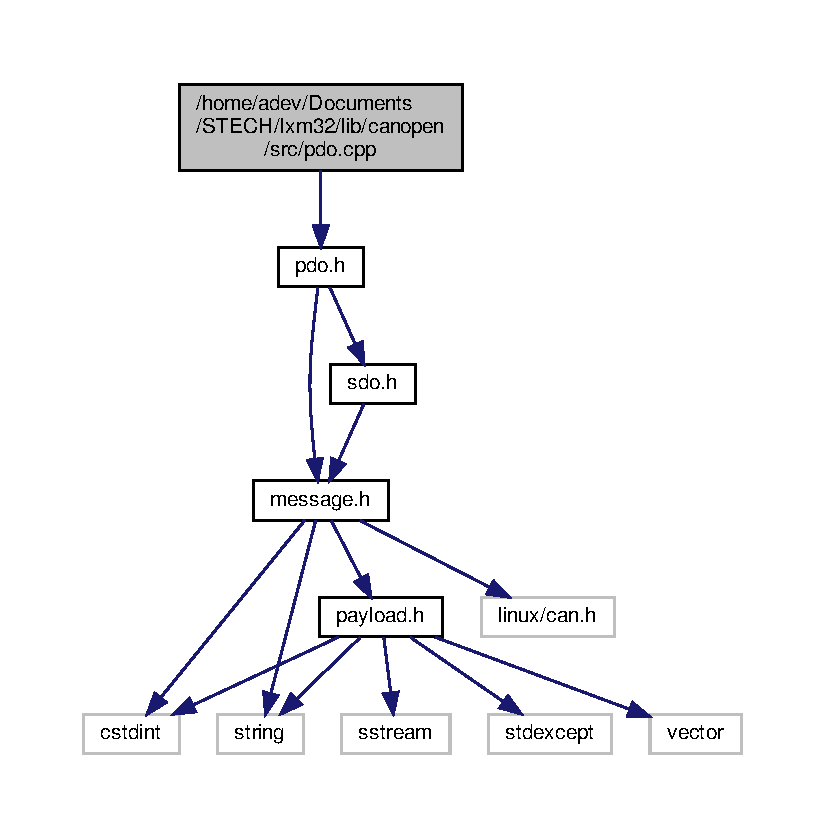
\includegraphics[width=350pt]{pdo_8cpp__incl}
\end{center}
\end{figure}
\subsection*{Namespaces}
\begin{DoxyCompactItemize}
\item 
 \hyperlink{namespace_c_a_nopen}{C\+A\+Nopen}
\end{DoxyCompactItemize}

\hypertarget{sdo_8cpp}{}\section{/home/adev/\+Documents/\+S\+T\+E\+C\+H/lxm32/lib/canopen/src/sdo.cpp File Reference}
\label{sdo_8cpp}\index{/home/adev/\+Documents/\+S\+T\+E\+C\+H/lxm32/lib/canopen/src/sdo.\+cpp@{/home/adev/\+Documents/\+S\+T\+E\+C\+H/lxm32/lib/canopen/src/sdo.\+cpp}}
{\ttfamily \#include \char`\"{}sdo.\+h\char`\"{}}\newline
{\ttfamily \#include $<$stdexcept$>$}\newline
Include dependency graph for sdo.\+cpp\+:\nopagebreak
\begin{figure}[H]
\begin{center}
\leavevmode
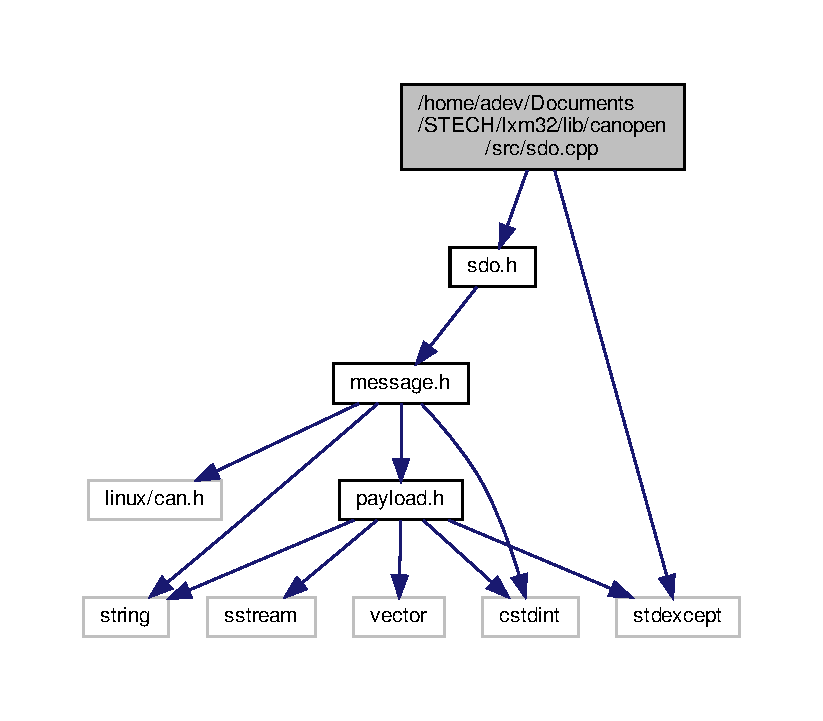
\includegraphics[width=350pt]{sdo_8cpp__incl}
\end{center}
\end{figure}
\subsection*{Namespaces}
\begin{DoxyCompactItemize}
\item 
 \hyperlink{namespace_c_a_nopen}{C\+A\+Nopen}
\end{DoxyCompactItemize}

\hypertarget{joystick_8h}{}\section{/home/adev/\+Documents/\+S\+T\+E\+C\+H/lxm32/lib/joystick/include/joystick.h File Reference}
\label{joystick_8h}\index{/home/adev/\+Documents/\+S\+T\+E\+C\+H/lxm32/lib/joystick/include/joystick.\+h@{/home/adev/\+Documents/\+S\+T\+E\+C\+H/lxm32/lib/joystick/include/joystick.\+h}}
{\ttfamily \#include $<$iostream$>$}\newline
{\ttfamily \#include $<$fcntl.\+h$>$}\newline
{\ttfamily \#include $<$pthread.\+h$>$}\newline
{\ttfamily \#include $<$math.\+h$>$}\newline
{\ttfamily \#include $<$linux/joystick.\+h$>$}\newline
{\ttfamily \#include $<$vector$>$}\newline
{\ttfamily \#include $<$unistd.\+h$>$}\newline
Include dependency graph for joystick.\+h\+:\nopagebreak
\begin{figure}[H]
\begin{center}
\leavevmode
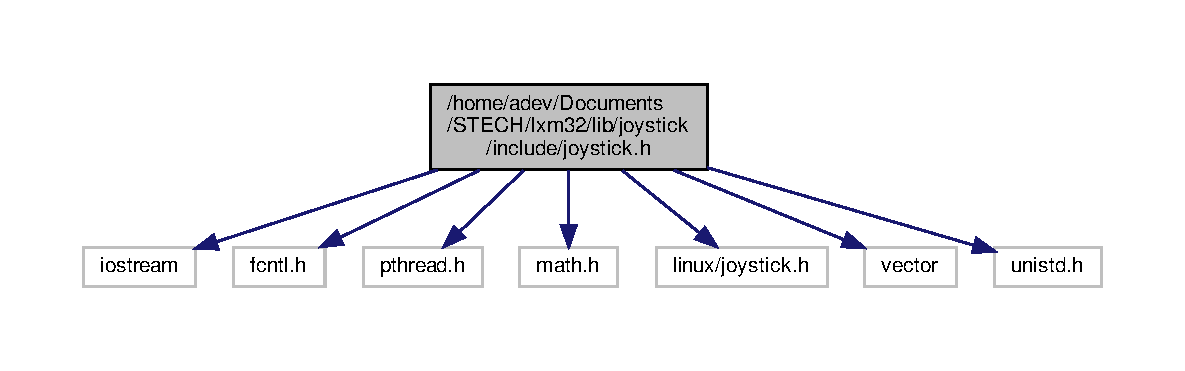
\includegraphics[width=350pt]{joystick_8h__incl}
\end{center}
\end{figure}
This graph shows which files directly or indirectly include this file\+:\nopagebreak
\begin{figure}[H]
\begin{center}
\leavevmode
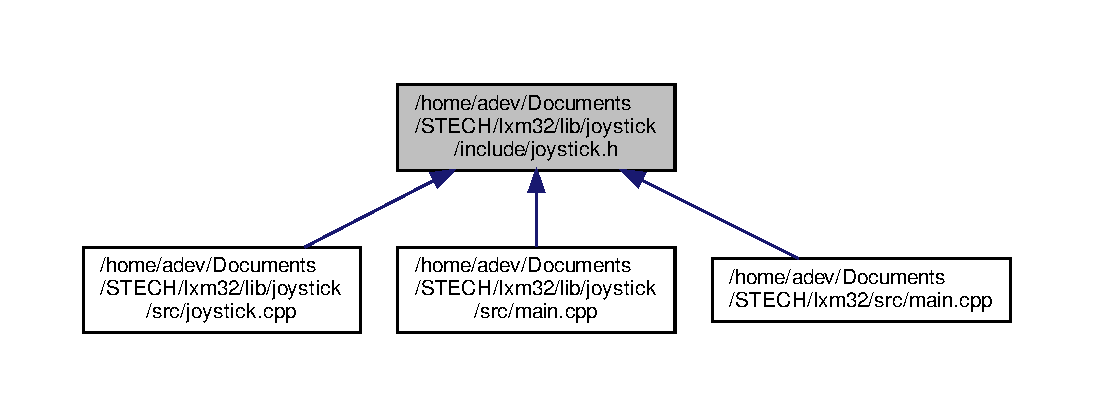
\includegraphics[width=350pt]{joystick_8h__dep__incl}
\end{center}
\end{figure}
\subsection*{Classes}
\begin{DoxyCompactItemize}
\item 
struct \hyperlink{structjoystick__position}{joystick\+\_\+position}
\item 
struct \hyperlink{structjoystick__state}{joystick\+\_\+state}
\item 
class \hyperlink{classc_joystick}{c\+Joystick}
\end{DoxyCompactItemize}
\subsection*{Macros}
\begin{DoxyCompactItemize}
\item 
\#define \hyperlink{joystick_8h_aa59cbb7e48c4f3c3dfbc694fd2869a3d}{J\+O\+Y\+S\+T\+I\+C\+K\+\_\+\+D\+EV}~\char`\"{}/dev/input/js0\char`\"{}
\end{DoxyCompactItemize}


\subsection{Macro Definition Documentation}
\mbox{\Hypertarget{joystick_8h_aa59cbb7e48c4f3c3dfbc694fd2869a3d}\label{joystick_8h_aa59cbb7e48c4f3c3dfbc694fd2869a3d}} 
\index{joystick.\+h@{joystick.\+h}!J\+O\+Y\+S\+T\+I\+C\+K\+\_\+\+D\+EV@{J\+O\+Y\+S\+T\+I\+C\+K\+\_\+\+D\+EV}}
\index{J\+O\+Y\+S\+T\+I\+C\+K\+\_\+\+D\+EV@{J\+O\+Y\+S\+T\+I\+C\+K\+\_\+\+D\+EV}!joystick.\+h@{joystick.\+h}}
\subsubsection{\texorpdfstring{J\+O\+Y\+S\+T\+I\+C\+K\+\_\+\+D\+EV}{JOYSTICK\_DEV}}
{\footnotesize\ttfamily \#define J\+O\+Y\+S\+T\+I\+C\+K\+\_\+\+D\+EV~\char`\"{}/dev/input/js0\char`\"{}}



Definition at line 12 of file joystick.\+h.


\hypertarget{joystick_8cpp}{}\section{/home/adev/\+Documents/\+S\+T\+E\+C\+H/lxm32/lib/joystick/src/joystick.cpp File Reference}
\label{joystick_8cpp}\index{/home/adev/\+Documents/\+S\+T\+E\+C\+H/lxm32/lib/joystick/src/joystick.\+cpp@{/home/adev/\+Documents/\+S\+T\+E\+C\+H/lxm32/lib/joystick/src/joystick.\+cpp}}
{\ttfamily \#include \char`\"{}joystick.\+h\char`\"{}}\newline
Include dependency graph for joystick.\+cpp\+:\nopagebreak
\begin{figure}[H]
\begin{center}
\leavevmode
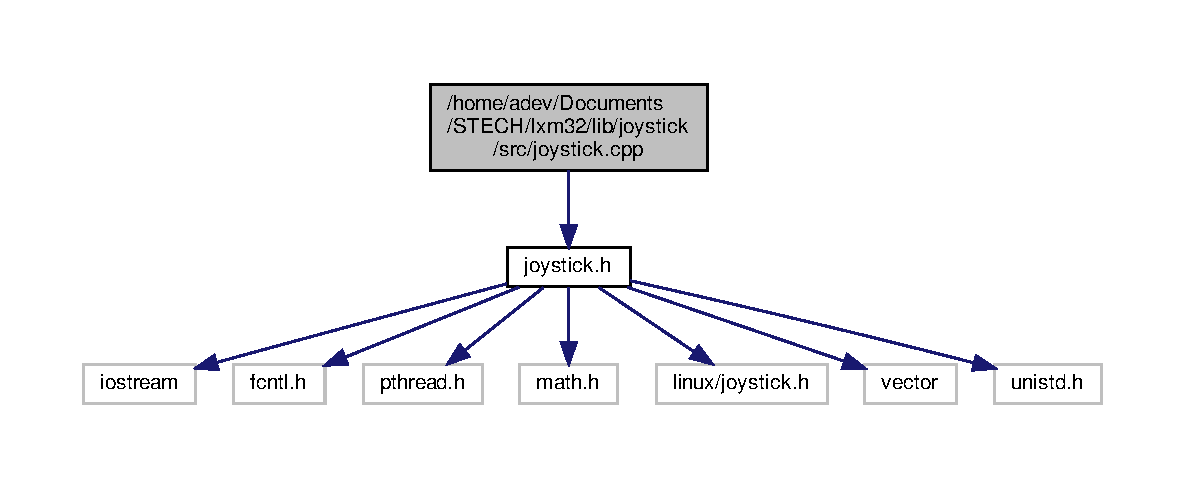
\includegraphics[width=350pt]{joystick_8cpp__incl}
\end{center}
\end{figure}

\hypertarget{_c_a_nopen__driver_8cpp}{}\section{/home/adev/\+Documents/\+S\+T\+E\+C\+H/lxm32/src/\+C\+A\+Nopen\+\_\+driver.cpp File Reference}
\label{_c_a_nopen__driver_8cpp}\index{/home/adev/\+Documents/\+S\+T\+E\+C\+H/lxm32/src/\+C\+A\+Nopen\+\_\+driver.\+cpp@{/home/adev/\+Documents/\+S\+T\+E\+C\+H/lxm32/src/\+C\+A\+Nopen\+\_\+driver.\+cpp}}
{\ttfamily \#include \char`\"{}C\+A\+Nopen\+\_\+driver.\+h\char`\"{}}\newline
Include dependency graph for C\+A\+Nopen\+\_\+driver.\+cpp\+:\nopagebreak
\begin{figure}[H]
\begin{center}
\leavevmode
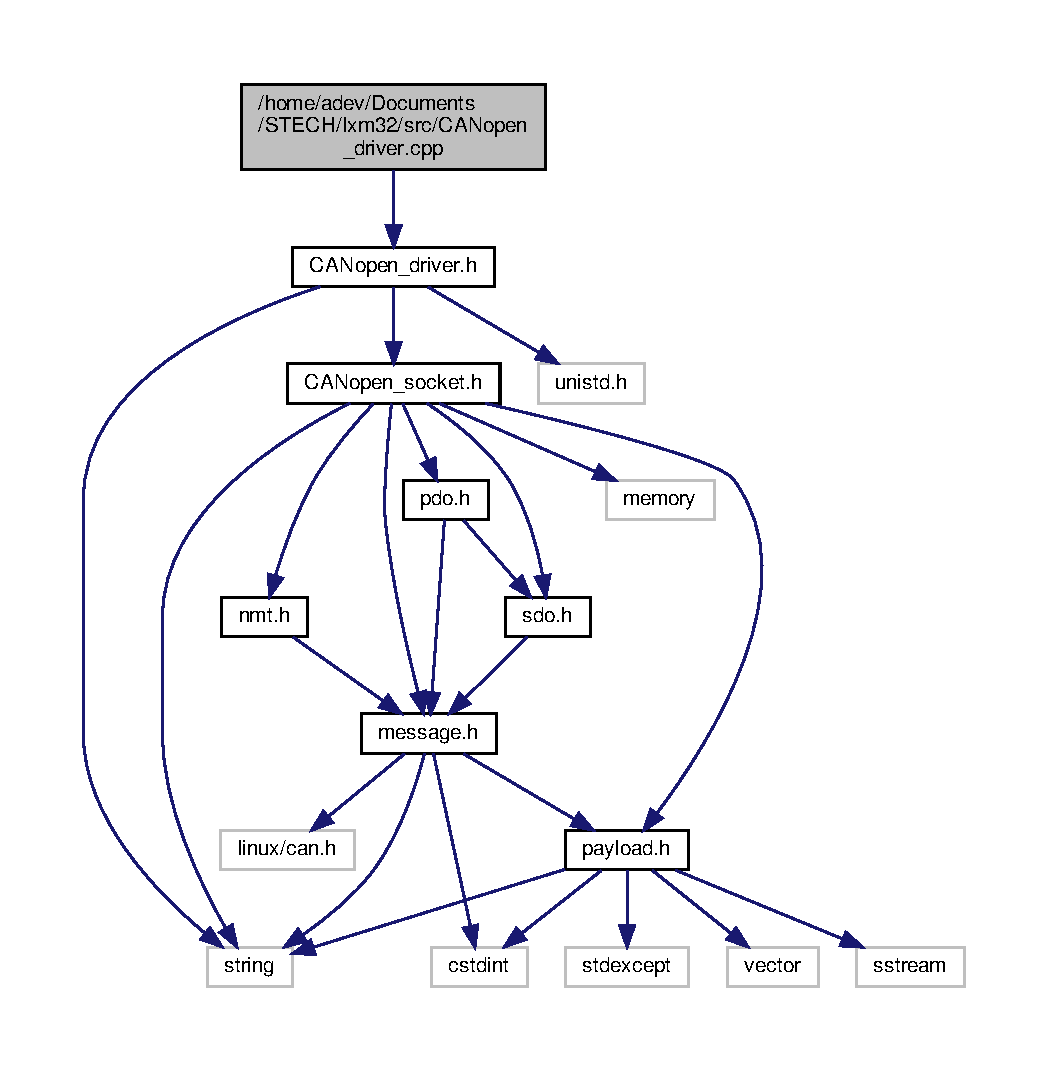
\includegraphics[width=350pt]{_c_a_nopen__driver_8cpp__incl}
\end{center}
\end{figure}

\hypertarget{_c_a_nopen__lxm32_8cpp}{}\section{/home/adev/\+Documents/\+S\+T\+E\+C\+H/lxm32/src/\+C\+A\+Nopen\+\_\+lxm32.cpp File Reference}
\label{_c_a_nopen__lxm32_8cpp}\index{/home/adev/\+Documents/\+S\+T\+E\+C\+H/lxm32/src/\+C\+A\+Nopen\+\_\+lxm32.\+cpp@{/home/adev/\+Documents/\+S\+T\+E\+C\+H/lxm32/src/\+C\+A\+Nopen\+\_\+lxm32.\+cpp}}
{\ttfamily \#include \char`\"{}C\+A\+Nopen\+\_\+lxm32.\+h\char`\"{}}\newline
Include dependency graph for C\+A\+Nopen\+\_\+lxm32.\+cpp\+:\nopagebreak
\begin{figure}[H]
\begin{center}
\leavevmode
\includegraphics[width=350pt]{_c_a_nopen__lxm32_8cpp__incl}
\end{center}
\end{figure}

%--- End generated contents ---

% Index
\backmatter
\newpage
\phantomsection
\clearemptydoublepage
\addcontentsline{toc}{chapter}{Index}
\printindex

\end{document}
